\documentclass[11pt]{book}

% \usepackage[showcrop,showframe,papersize={5.5in,8.5in}]{geometry}
\usepackage[papersize={5.5in,8.5in},bindingoffset=.25in]{geometry}

\usepackage{xifthen}
\usepackage{makeidx}
\makeindex
\usepackage[nottoc]{tocbibind}
\usepackage[font=footnotesize]{idxlayout}

\usepackage{fancyhdr}

\renewcommand{\chaptermark}[1]{\markboth{#1}{}}
\renewcommand{\sectionmark}[1]{\markright{#1}}

\setcounter{tocdepth}{1}

\usepackage{fontspec}
\setmainfont[Ligatures={Common,TeX}, Numbers=OldStyle]{TeX Gyre Schola}

\usepackage{microtype}

\usepackage{hyperref}

\usepackage{graphicx}

\usepackage[all]{nowidow}

\hyphenation{Na-po-le-on-ic}
\hyphenation{stra-te-gic-al}
\hyphenation{ap-proached}
\hyphenation{Chat-ham}
\hyphenation{re-serve}

\newcommand{\warcourse}[2]{%
  \begin{center}
  {\Large \textbf{War Course} \\[1em]}%
  \section[#1]{#2}%
  \end{center}
}

\newcommand{\note}{\textbf{Note.}---}
\newcommand{\example}{\textbf{Example.}---}
\newcommand{\result}{\textbf{Result.}---}

\newcommand{\idx}[2][]{%
 \ifthenelse{\isempty{#1}}{%
   #2\index{#2}%
 }{%
   #1\index{#2}%
 }%
}

\newcommand{\simpletitle}{Some Principles \\ of \\ Maritime Strategy}
\title{\simpletitle}

\author{Julian Stafford Corbett \\[1em] London \\[1em] 1911}

\date{}

\begin{document}

\emergencystretch 2em%

\setlength{\baselineskip}{1.2\baselineskip}
\frontmatter

\thispagestyle{empty}
\hspace{0pt}
\vfill
\begin{center}
  \Large
  \simpletitle
\end{center}
\vfill

\pagebreak
\thispagestyle{empty}

\hspace{0pt}
\vfill

\emph{\href{http://www.gutenberg.org/ebooks/15076}{http://www.gutenberg.org/ebooks/15076}}

\emph{This eBook is for the use of anyone anywhere in the \idx{United States} and
most other parts of the world at no cost and with almost no
restrictions whatsoever. You may copy it, give it away or re-use it
under the terms of the Project Gutenberg License included with this
eBook or online at www.gutenberg.org. If you are not located in the
\idx{United States}, you'll have to check the laws of the country where you
are located before using this ebook.}

\pagebreak
\thispagestyle{empty}
\hspace{0pt}

\pagebreak
\thispagestyle{empty}
\hspace{0pt}
\vfill

% [Illustration: \emph{Sir Julian Corbett (courtesy D.M. Schurman)}]
\begin{figure}[ht!]
\centering
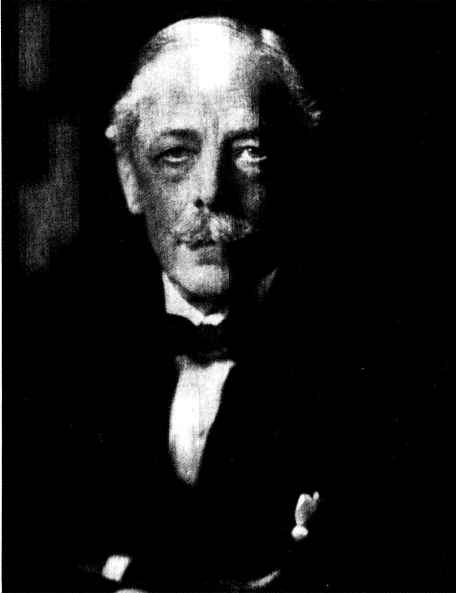
\includegraphics[width=70mm]{001.jpg}
\caption{Sir Julian Corbett (courtesy D.M. Schurman)}
\end{figure}

\vfill

\maketitle

\thispagestyle{empty}
\hspace{0pt}
\vfill

\noindent E-text prepared by Suzanne Shell, \idx[Keith]{Keith, Admiral Lord} Edkins, and the Project Gutenberg Online Distributed Proofreading Team

\noindent Typeset by Tommy M. McGuire using \LaTeX $2_\epsilon$.

\noindent The font is \TeX\ Gyre Schola.

\pagebreak

\tableofcontents

\chapter[The Theoretical Study of War]{The Theoretical Study of War---Its Use and Limitations}

At first sight nothing can appear more unpractical, less promising of   
useful result, than to approach the study of war with a theory. There   
seems indeed to be something essentially antagonistic between the habit 
of mind that seeks theoretical guidance and that which makes for the    
successful conduct of war. The conduct of war is so much a question     
of personality, of character, of common-sense, of rapid decision upon   
complex and ever-shifting factors, and those factors themselves are so  
varied, so intangible, so dependent upon unstable moral and physical    
conditions, that it seems incapable of being reduced to anything like   
true scientific analysis. At the bare idea of a theory or ``science''   
of war the mind recurs uneasily to well-known cases where highly        
``scientific'' officers failed as leaders. Yet, on the other hand, no   
one will deny that since the great theorists of the early nineteenth    
century attempted to produce a reasoned \idx[theory of war]{Theory of   
war}, its planning and conduct have acquired a method, a precision, and 
a certainty of grasp which were unknown before. Still less will any one 
deny the value which the shrewdest and most successful leaders in war   
have placed upon the work of the classical strategical writers.         

The truth is that the mistrust of theory arises from a misconception    
of what it is that theory claims to do. It does not pretend to give     
the power of conduct in the field; it claims no more than to increase   
the effective power of conduct. Its main practical value is that it     
can assist a capable man to acquire a broad outlook whereby he may      
be the surer his plan shall cover all the ground, and whereby he may    
with greater rapidity and certainty seize all the factors of a sudden   
situation. The greatest of the theorists himself puts the matter quite  
frankly. Of theoretical study he says, ``It should educate the mind of  
the man who is to lead in war, or rather guide him to self-education,   
but it should not accompany him on the field of battle.''               

Its practical utility, however, is not by any means confined to its     
effects upon the powers of a leader. It is not enough that a leader     
should have the ability to decide rightly; his subordinates must seize  
at once the full meaning of his decision and be able to express it with 
certainty in well-adjusted action. For this every man concerned must    
have been trained to think in the same plane; the chief's order must    
awake in every brain the same process of thought; his words must have   
the same meaning for all. If a theory of tactics had existed in 1780,   
and if Captain \idx[Carkett]{Carkett, Captain Robert} had had a sound   
training in such a theory, he could not possibly have misunderstood     
\idx[Rodney]{Rodney, Admiral Sir George B.}'s signal. As it was, the    
real intention of the signal was obscure, and \idx[Rodney]{Rodney,      
Admiral Sir George B.}'s neglect to explain the tactical device it      
indicated robbed his country of a victory at an hour of the direst      
need. There had been no previous theoretical training to supply the     
omission, and \idx[Rodney]{Rodney, Admiral Sir George B.}'s fine        
conception was unintelligible to anybody but himself.                   

Nor is it only for the sake of mental solidarity between a chief and    
his subordinates that theory is indispensable. It is of still higher    
value for producing a similar solidarity between him and his superiors  
at the Council table at home. How often have officers dumbly acquiesced 
in ill-advised operations simply for lack of the mental power and       
verbal apparatus to convince an impatient Minister where the errors     
of his plan lay? How often, moreover, have statesmen and officers,      
even in the most harmonious conference, been unable to decide on a      
coherent plan of war from inability to analyse scientifically the       
situation they had to face, and to recognise the general character of   
the struggle in which they were about to engage. That the true nature   
of a war should be realised by contemporaries as clearly as it comes    
to be seen afterwards in the fuller light of history is seldom to be    
expected. At close range accidental factors will force themselves into  
undue prominence and tend to obscure the true horizon. Such error can   
scarcely ever be eliminated, but by theoretical study we can reduce     
it, nor by any other means can we hope to approach the clearness of     
vision with which posterity will read our mistakes. Theory is, in fact, 
a question of education and deliberation, and not of execution at all.  
That depends on the combination of intangible human qualities which we  
call executive ability.                                                 

This, then, is all the great authorities ever claimed for theory,       
but to this claim the chief of them at least, after years of active     
service on the Staff, attached the highest importance. ``In actual      
operations,'' he wrote in one of his latest memoranda, ``men are        
guided solely by their judgment, and it will hit the mark more or less  
accurately according as they possess more or less genius. This is       
the way all great generals have acted.... Thus it will always be in     
action, and so far judgment will suffice. But when it is a question     
not of taking action yourself, but of convincing others at the Council  
table, then everything depends on clear conceptions and the exposition  
of the inherent relations of things. So little progress has been made   
in this respect that most deliberations are merely verbal contentions   
which rest on no firm foundation, and end either in every one retaining 
his own opinion, or in a compromise from considerations of mutual       
respect---a middle course of no actual value.''\footnote{Clausewitz,    
\emph{\idx[On War]{Clausewitz, General Karl von!\emph{On War}}}, p.~ix. 
The references are to Colonel Graham's translation of the third German  
edition, but his wording is not always followed exactly.}               

The writer's experience of such discussions was rich and at first       
hand. Clear conceptions of the ideas and factors involved in a war      
problem, and a definite exposition of the relations between them,       
were in his eyes the remedy for loose and purposeless discussion; and   
such conceptions and expositions are all we mean by the theory or the   
science of war. It is a process by which we co-ordinate our ideas,      
define the meaning of the words we use, grasp the difference between    
essential and unessential factors, and fix and expose the fundamental   
data on which every one is agreed. In this way we prepare the apparatus 
of practical discussion; we secure the means of arranging the factors   
in manageable shape, and of deducing from them with precision and       
rapidity a practical course of action. Without such an apparatus no two 
men can even think on the same line; much less can they ever hope to    
detach the real point of difference that divides them and isolate it    
for quiet solution.                                                     

In our own case this view of the value of strategical theory has        
a special significance, and one far wider than its continental          
enunciators contemplated. For a world-wide maritime Empire the          
successful conduct of war will often turn not only on the decisions     
of the Council chamber at home, but on the outcome of conferences       
in all parts of the world between squadronal commanders and the         
local authorities, both civil and military, and even between            
commanders-in-chief of adjacent stations. In time of war or of          
preparation for war, in which the Empire is concerned, arrangements     
must always be based to an exceptional degree on the mutual relation    
of naval, military, and political considerations. The line of mean      
efficiency, though indicated from home, must be worked out locally, and 
worked out on factors of which no one service is master. Conference     
is always necessary, and for conference to succeed there must be a      
common vehicle of expression and a common plane of thought. It is for   
this essential preparation that theoretical study alone can provide;    
and herein lies its practical value for all who aspire to the higher    
responsibilities of the Imperial service.                               

So great indeed is the value of abstract strategical study from this point
of view, that it is necessary to guard ourselves against over-valuation. So
far from claiming for their so-called science more than the possibilities
we have indicated, the classical strategists insist again and again on the
danger of seeking from it what it cannot give. They even repudiate the very
name of ``Science.'' They prefer the older term ``Art.'' They will permit no
laws or rules. Such laws, they say, can only mislead in practice, for the
friction to which they are subject from the incalculable human factors
alone is such that the friction is stronger than the law. It is an old
adage of lawyers that nothing is so misleading as a legal maxim, but a
strategical maxim is undoubtedly and in every way less to be trusted in
action.

What then, it will be asked, are the tangible results which we can hope to
attain from theory? If all on which we have to build is so indeterminate,
how are any practical conclusions to be reached? That the factors are
infinitely varied and difficult to determine is true, but that, it must be
remembered, is just what emphasises the necessity of reaching such firm
standpoints as are attainable. The vaguer the problem to be solved, the
more resolute must we be in seeking points of departure from which we can
begin to lay a course, keeping always an eye open for the accidents that
will beset us, and being always alive to their deflecting influences. And
this is just what the theoretical study of strategy can do. It can at least
determine the normal. By careful collation of past events it becomes clear
that certain lines of conduct tend normally to produce certain effects;
that wars tend to take certain forms each with a marked idiosyncrasy; that
these forms are normally related to the object of the war and to its value
to one or both belligerents; that a system of operations which suits one
form may not be that best suited to another. We can even go further. By
pursuing an historical and comparative method we can detect that even the
human factor is not quite indeterminable. We can assert that certain
situations will normally produce, whether in ourselves or in our
adversaries, certain moral states on which we may calculate.

Having determined the normal, we are at once in a stronger position. Any
proposal can be compared with it, and we can proceed to discuss clearly the
weight of the factors which prompt us to depart from the normal. Every case
must be judged on its merits, but without a normal to work from we cannot
form any real judgment at all; we can only guess. Every case will assuredly
depart from the normal to a greater or less extent, and it is equally
certain that the greatest successes in war have been the boldest departures
from the normal. But for the most part they have been departures made with
open eyes by geniuses who could perceive in the accidents of the case a
just reason for the departure.

Take an analogous example, and the province of stra\-te\-gic\-al theory becomes
clear at once. Navigation and the parts of seamanship that belong to it
have to deal with phenomena as varied and unreliable as those of the
conduct of war. Together they form an art which depends quite as much as
generalship on the judgment of individuals. The law of storms and tides, of
winds and currents, and the whole of meteorology are subject to infinite
and incalculable deflections, and yet who will deny nowadays that by the
theoretical study of such things the seaman's art has gained in coherence
and strength? Such study will not by itself make a seaman or a navigator,
but without it no seaman or navigator can nowadays pretend to the name.
Because storms do not always behave in the same way, because currents are
erratic, will the most practical seaman deny that the study of the normal
conditions are useless to him in his practical decisions?

If, then, the theoretical study of strategy be ap\-proached in this way---if,
that is, it be regarded not as a sub\-stit\-ute for judgment and experience,
but as a means of fertilising both, it can do no man harm. Individual
thought and common-sense will remain the masters and remain the guides to
point the general direction when the mass of facts begins to grow
bewildering. Theory will warn us the moment we begin to leave the beaten
track, and enable us to decide with open eyes whether the divergence is
necessary or justifiable. Above all, when men assemble in Council it will
hold discussion to the essential lines, and help to keep side issues in
their place.

But beyond all this there lies in the \idx[theory of war]{Theory        
of war} yet another element of peculiar value to a maritime             
Empire. We are accustomed, partly for convenience and partly            
from lack of a scientific habit of thought, to speak of naval           
\idx[strategy]{Strategy!naval and maritime} and military strategy as    
though they were distinct branches of knowledge which had no common     
ground. It is the \idx[theory of war]{Theory of war} which brings       
out their intimate relation. It reveals that embracing them both is     
a larger \idx[strategy]{Strategy!naval and maritime} which regards      
the fleet and army as one weapon, which co-ordinates their action,      
and indicates the lines on which each must move to realise the full     
power of both. It will direct us to assign to each its proper function  
in a plan of war; it will enable each service to realise the better     
the limitations and the possibilities of the function with which it     
is charged, and how and when its own necessities must give way to a     
higher or more pressing need of the other. It discloses, in short,      
that naval \idx[strategy]{Strategy!naval and maritime} is not a         
thing by itself, that its problems can seldom or never be solved on     
naval considerations alone, but that it is only a part of maritime      
\idx[strategy]{Strategy!naval and maritime}---the higher learning which 
teaches us that for a maritime State to make successful war and to      
realise her special strength, army and navy must be used and thought    
of as instruments no less intimately connected than are the three arms  
ashore.                                                                 

It is for these reasons that it is of little use to approach naval      
\idx[strategy]{Strategy!naval and maritime} except through the          
\idx[theory of war]{Theory of war}. Without such theory we can never    
really understand its scope or meaning, nor can we hope to grasp the    
forces which most profoundly affect its conclusions.                    

\mainmatter

\part{Theory of War}

\chapter{The Theory of War}

The last thing that an explorer arrives at is a complete map that       
will cover the whole ground he has travelled, but for those who         
come after him and would profit by and extend his knowledge his         
map is the first thing with which they will begin. So it is with        
\idx[strategy]{Strategy!naval and maritime}. Before we start upon its   
study we seek a chart which will show us at a glance what exactly is    
the ground we have to cover and what are the leading features which     
determine its form and general characteristics. Such a chart a ``theory 
of war'' alone can provide. It is for this reason that in the study     
of war we must get our theory clear before we can venture in search     
of practical conclusions. So great is the complexity of war that        
without such a guide we are sure to go astray amidst the bewildering    
multiplicity of tracks and obstacles that meet us at every step. If     
for continental strategy its value has been proved abundantly, then     
for maritime \idx[strategy]{Strategy!naval and maritime}, where the     
conditions are far more complex, the need of it is even greater.        

By maritime \idx[strategy]{Strategy!naval and maritime} we mean the     
principles which govern a war in which the sea is a substantial         
factor. Naval \idx[strategy]{Strategy!naval and maritime} is but that   
part of it which determines the movements of the fleet when maritime    
\idx[strategy]{Strategy!naval and maritime} has determined what part    
the fleet must play in relation to the action of the land forces; for   
it scarcely needs saying that it is almost impossible that a war can    
be decided by naval action alone. Unaided, naval pressure can only      
work by a process of exhaustion. Its effects must always be slow,       
and so galling both to our own commercial community and to neutrals,    
that the tendency is always to accept terms of peace that are far       
from conclusive. For a firm decision a quicker and more drastic         
form of pressure is required. Since men live upon the land and not      
upon the sea, great issues between nations at war have always been      
decided---except in the rarest cases---either by what your army can do  
against your enemy's territory and national life or else by the fear of 
what the fleet makes it possible for your army to do.                   

The paramount concern, then, of maritime \idx[strategy]{Strategy!naval  
and maritime} is to determine the mutual relations of your army and     
navy in a plan of war. When this is done, and not till then, naval      
\idx[strategy]{Strategy!naval and maritime} can begin to work out the   
manner in which the fleet can best discharge the function assigned to   
it.                                                                     

The problem of such co-ordination is one that is susceptible of widely
varying solutions. It may be that the command of the sea is of so urgent an
importance that the army will have to devote itself to assisting the fleet
in its special task before it can act directly against the enemy's
territory and land forces; on the other hand, it may be that the immediate
duty of the fleet will be to forward military action ashore before it is
free to devote itself whole-heartedly to the destruction of the enemy's
fleets. The crude maxims as to primary objects which seem to have served
well enough in continental warfare have never worked so clearly where the
sea enters seriously into a war. In such cases it will not suffice to say
the primary object of the army is to destroy the enemy's army, or that of
the fleet to destroy the enemy's fleet. The delicate interactions of the
land and sea factors produce conditions too intricate for such blunt
solutions. Even the initial equations they present are too complex to be
reduced by the simple application of rough-and-ready maxims. Their right
handling depends upon the broadest and most fundamental principles of war,
and it is as a standpoint from which to get a clear and unobstructed view
of the factors in their true relations that a \idx[theory of war]{Theory of war} has perhaps its
highest value.

The theory which now holds the field is that war in a fundamental sense is
a continuation of policy by other means. The process by which the
continental strategists arrived at it involved some hard philosophical
reasoning. Practical and experienced veterans as they were, their method is
not one that works easily with our own habit of thought. It will be well,
therefore, to endeavour first to present their conclusions in a concrete
form, which will make the pith of the matter intelligible at once. Take,
now, the ordinary case of a naval or military Staff being asked to prepare
a war plan against a certain State and to advise what means it will
require. To any one who has considered such matters it is obvious the reply
must be another question---What will the war be about? Without a definite
answer or alternative answers to that question a Staff can scarcely do more
than engage in making such forces as the country can afford as efficient as
possible. Before they take any sure step further they must know many
things. They must know whether they are expected to take something from the
enemy, or to prevent his taking something either from us or from some other
State. If from some other State, the measures to be taken will depend on
its geographical situation and on its relative strength by land and sea.
Even when the object is clear it will be necessary to know how much value
the enemy attaches to it. Is it one for which he will be likely to fight to
the death, or one which he will abandon in the face of comparatively slight
resistance? If the former, we cannot hope to succeed without entirely
overthrowing his powers of resistance. If the latter, it will suffice, as
it often has sufficed, to aim at something less costly and hazardous and
better within our means. All these are questions which lie in the lap of
Ministers charged with the foreign policy of the country, and before the
Staff can proceed with a war plan they must be answered by Ministers.

In short, the Staff must ask of them what is the policy which your
diplomacy is pursuing, and where, and why, do you expect it to break down
and force you to take up arms? The Staff has to carry on in fact when
diplomacy has failed to achieve the object in view, and the method they
will use will depend on the nature of that object. So we arrive crudely at
our theory that war is a continuation of policy, a form of political
intercourse in which we fight battles instead of writing notes.

It was this theory, simple and even meaningless as it appears at first
sight, that gave the key to the practical work of framing a modern war plan
and revolutionised the study of strategy. It was not till the beginning of
the nineteenth century that such a theory was arrived at. For centuries men
had written on the ``Art of War,'' but for want of a working theory their
labours as a whole had been unscientific, concerned for the most part with
the discussion of passing fashions and the elaboration of platitudes. Much
good work it is true was done on details, but no broad outlook had been
obtained to enable us to determine their relation to the fundamental
constants of the subject. No standpoint had been found from which we could
readily detach such constants from what was merely accidental. The result
was a tendency to argue too exclusively from the latest examples and to
become entangled in erroneous thought by trying to apply the methods which
had attained the last success to war as a whole. There was no means of
determining how far the particular success was due to special conditions
and how far it was due to factors common to all wars.

It was the \idx[Revolutionary]{Revolution, French} and \idx[Napoleonic]{Napoleon!methods} wars, coinciding as they did with a
period of philosophic activity, that revealed the shallowness and empirical
nature of all that had been done up to that time. \idx{Napoleon}'s methods
appeared to his contemporaries to have produced so strenuous a revolution
in the conduct of land warfare that it assumed a wholly new aspect, and it
was obvious that those conceptions which had sufficed previously had become
inadequate as a basis of sound study. War on land seemed to have changed
from a calculated affair of thrust and parry between standing armies to a
headlong rush of one nation in arms upon another, each thirsting for the
other's life, and resolved to have it or perish in the attempt. Men felt
themselves faced with a manifestation of human energy which had had no
counterpart, at least in civilised times.

The assumption was not entirely true. For although the Continent had never
before adopted the methods in question, our own country was no stranger to
them either on sea or land. As we shall see, our own Revolution in the
seventeenth century had produced strenuous methods of making war which were
closely related to those which \idx{Napoleon} took over from the French
\idx[Revolutionary]{Revolution, French} leaders. A more philosophic outlook might have suggested that
the phenomenon was not really exceptional, but rather the natural outcome
of popular energy inspired by a stirring political ideal. But the British
precedent was forgotten, and so profound was the disturbance caused by the
new French methods that its effects are with us still. We are in fact still
dominated by the idea that since the \idx[Napoleonic]{Napoleon!methods} era war has been
essentially a different thing. Our teachers incline to insist that there is
now only one way of making war, and that is \idx{Napoleon}'s way. Ignoring the
fact that he failed in the end, they brand as heresy the bare suggestion
that there may be other ways, and not content with assuming that his system
will fit all land wars, however much their natures and objects may differ,
they would force naval warfare into the same uniform under the impression
apparently that they are thereby making it presentable and giving it some
new force.

Seeing how cramping the \idx[Napoleonic]{Napoleon!methods} idea has become, it will be convenient
before going further to determine its special characteristics exactly, but
that is no easy matter. The moment we approach it in a critical spirit, it
begins to grow nebulous and very difficult to define. We can dimly make out
four distinct ideas mingled in the current notion. First, there is the idea
of making war not merely with a professional standing army, but with the
whole armed nation---a conception which of course was not really \idx{Napoleon}'s.
It was inherited by him from the \idx[Revolution]{Revolution, French}, but was in fact far older. It
was but a revival of the universal practice which obtained in the barbaric
stages of social development, and which every civilisation in turn had
abandoned as economically unsound and subversive of specialisation in
citizenship. The results of the abandonment were sometimes good and
sometimes bad, but the determining conditions have been studied as yet too
imperfectly to justify any broad generalisation. Secondly, there is the
idea of strenuous and persistent effort---not resting to secure each minor
advantage, but pressing the enemy without pause or rest till he is utterly
overthrown---an idea in which \idx[Cromwell]{Cromwell, Oliver} had anticipated \idx{Napoleon} by a century
and a half. Scarcely distinguishable from this is a third idea---that of
taking the offensive, in which there was really nothing new at all, since
its advantages had always been understood, and \idx[Frederick]{Frederick the Great} the Great had
pressed it to extremity with little less daring than \idx{Napoleon} himself---nay
even to culpable rashness, as the highest exponents of the \idx[Napoleonic]{Napoleon!methods} idea
admit. Finally, there is the notion of making the armed forces of the enemy
and not his territory or any part of it your main objective. This perhaps
is regarded as the strongest characteristic of \idx[Napoleonic]{Napoleon!methods}'s methods, and yet
even here we are confused by the fact that undoubtedly on some very
important occasions---the \idx{Austerlitz campaign}, for example---\idx[Napoleon]{Napoleon!methods} made
the hostile capital his objective as though he believed its occupation was
the most effective step towards the overthrow of the enemy's power and will
to resist. He certainly did not make the enemy's main army his primary
objective---for their main army was not \idx[Mack]{Mack, General}'s but that of the Archduke
\idx[Charles]{Charles of Austria}.

On the whole then, when men speak of the \idx[Napoleonic]{Napoleon!methods} system they seem to
include two groups of ideas---one which comprises the conception of war made
with the whole force of the nation; the other, a group which includes the
\idx[Cromwellian]{Cromwell, Oliver} idea of persistent effort, \idx[Frederick]{Frederick the Great}'s preference for the
offensive at almost any risk, and finally the idea of the enemy's armed
forces as the main objective, which was also \idx[Cromwell]{Cromwell, Oliver}'s.

It is the combination of these by no means original or very distinct ideas
that we are told has brought about so entire a change in the conduct of war
that it has become altogether a different thing. It is unnecessary for our
purpose to consider how far the facts seem to support such a conclusion,
for in the inherent nature of things it must be radically unsound. Neither
war nor anything else can change in its essentials. If it appears to do so,
it is because we are still mistaking accidents for essentials, and this is
exactly how it struck the acutest thinkers of \idx[Napoleonic]{Napoleon!methods} times.

For a while it is true they were bewildered, but so soon as they had had
time to clear their heads from the din of the struggle in which they had
taken part, they began to see that the new phenomena were but accidents
after all. They perceived that \idx[Napoleon]{Napoleon!methods}'s methods, which had taken the
world by storm, had met with success in wars of a certain nature only, and
that when he tried to extend those methods to other natures of war he had
met with failure and even disaster. How was this to be explained? What
theory, for instance, would cover Napoleon's successes in Germany and
Italy, as well as his failures in Spain and Russia? If the whole conception
of war had changed, how could you account for the success of England, who
had not changed her methods? To us the answer to these questions is of
living and infinite importance. Our standpoint remains still unchanged. Is
there anything inherent in the conception of war that justifies that
attitude in our case? Are we entitled to expect from it again the same
success it met with in the past?

The first man to enunciate a theory which would explain the phenomena   
of the \idx[Napoleonic]{Napoleon!methods} era and co-ordinate them with 
previous history was General Carl von \idx[Clausewitz]{Clausewitz,      
General Karl von}, a man whose arduous service on the Staff and         
the actual work of higher instruction had taught the necessity of       
systematising the study of his profession. He was no mere professor,    
but a soldier bred in the severest school of war. The pupil and         
friend of \idx[Sharnhorst]{Sharnhorst, General Gerhard von} and         
\idx[Gneisenau]{Gneisenau, Field Marshal August von}, he had served     
on the Staff of \idx[Bl�cher]{Blucher, Field Marshal Gebhard            
von@Bl\"ucher, Field Marshal Gebhard von} in 1813, he had been Chief    
of the Staff to Wallmoden in his campaign against \idx[Davout]{Davout,  
Louis-Nicolas} on the Lower Elbe, and also to the Third \idx{Prussia}n  
Army Corps in the campaign of 1815. Thereafter for more than ten years  
he was Director of the General Academy of War at Berlin, and died in    
1831 as Chief of the Staff to Marshal \idx[Gneisenau]{Gneisenau, Field  
Marshal August von}. For the fifty years that followed his death his    
theories and system were, as he expected they would be, attacked from   
all sides. Yet to-day his work is more firmly established than ever as  
the necessary basis of all strategical thought, and above all in the    
``blood and iron'' school of Germany.                                   

The process by which he reached his famous theory can be followed       
in his classical work \emph{\idx[On War]{Clausewitz, General Karl       
von!\emph{On War}}} and the \emph{Notes} regarding it which he left     
behind him. In accordance with the philosophic fashion of his time he   
began by trying to formulate an abstract idea of war. The definition    
he started with was that ``War is an act of violence to compel our      
opponent to do our will.'' But that act of violence was not merely      
``the shock of armies,'' as Montecuccoli had defined it a century       
and a half before. If the abstract idea of war be followed to its       
logical conclusion, the act of violence must be performed with the      
whole of the means at our disposal and with the utmost exertion of our  
will. Consequently we get the conception of two armed nations flinging  
themselves one upon the other, and continuing the struggle with the     
utmost strength and energy they can command till one or other is no     
longer capable of resistance. This \idx[Clausewitz]{Clausewitz, General 
Karl von} called ``\idx{Absolute War}.'' But his practical experience   
and ripe study of history told him at once that ``\idx[Real War]{``Real 
War''}'' was something radically different. It was true, as he said,    
that \idx[Napoleon]{Napoleon!methods}'s methods had approximated to the 
absolute and had given some colour to the use of the absolute idea as   
a working theory. ``But shall we,'' he acutely asks, ``rest satisfied   
with this idea and judge all wars by it however much they may differ    
from it---shall we deduce from it all the requirements of theory? We    
must decide the point, for we can say nothing trustworthy about a       
war plan until we have made up our minds whether war should only be     
of this kind or whether it may be of another kind.'' He saw at once     
that a theory formed upon the abstract or absolute idea of war would    
not cover the ground, and therefore failed to give what was required    
for practical purposes. It would exclude almost the whole of war from   
Alexander's time to \idx{Napoleon}'s. And what guarantee was there that 
the next war would confirm to the \idx[Napoleonic]{Napoleon!methods}    
type and accommodate itself to the abstract theory? ``This theory,'' he 
says, ``is still quite powerless against the force of circumstances.''  
And so it proved, for the wars of the middle nineteenth century did in  
fact revert to the pre-Napoleonic type.                                 

In short, \idx[Clausewitz]{Clausewitz, General Karl von!theory}'s       
difficulty in adopting his abstract theory as a working rule was        
that his practical mind could not forget that war had not begun with    
the \idx[Revolutionary]{Revolution, French} era, nor was it likely      
to end with it. If that era had changed the conduct of war, it must     
be presumed that war would change again with other times and other      
conditions. A \idx[theory of war]{Theory of war} which did not allow    
for this and did not cover all that had gone before was no theory at    
all. If a \idx[theory of war]{Theory of war} was to be of any use       
as a practical guide it must cover and explain not only the extreme     
manifestation of hostility which he himself had witnessed, but every    
manifestation that had occurred in the past or was likely to recur in   
the future.                                                             

It was in casting about for the underlying causes of the oscillations
manifested in the energy and intensity of hostile relations that he found
his solution. His experience on the Staff, and his study of the inner
springs of war, told him it was never in fact a question of purely military
endeavour aiming always at the extreme of what was possible or expedient
from a purely military point of view. The energy exhibited would always be
modified by political considerations and by the depth of the national
interest in the object of the war. He saw that real war was in fact an
international relation which differed from other international relations
only in the method we adopted to achieve the object of our policy. So it
was he arrived at his famous theory---``that war is a mere continuation of
policy by other means.''

At first sight there seems little enough in it. It may seem perhaps that we
have been watching a mountain in labour and nothing but a mouse has been
produced. But it is only upon some such simple, even obvious, formula that
any scientific system can be constructed with safety. We have only to
develop the meaning of this one to see how important and practical are the
guiding lines which flow from it.

With the conception of war as a continuation of political intercourse   
before us, it is clear that everything which lies outside the political 
conception, everything, that is, which is strictly peculiar to military 
and naval operations, relates merely to the means which we use to       
achieve our policy. Consequently, the first desideratum of a war plan   
is that the means adopted must conflict as little as possible with      
the political conditions from which the war springs. In practice,       
of course, as in all human relations, there will be a compromise        
between the means and the end, between the political and the military   
exigencies. But \idx[Clausewitz]{Clausewitz, General Karl von!theory}   
held that policy must always be the master. The officer charged with    
the conduct of the war may of course demand that the tendencies and     
views of policy shall not be incompatible with the military means which 
are placed at his disposal; but however strongly this demand may react  
on policy in particular cases, military action must still be regarded   
only as a manifestation of policy. It must never supersede policy. The  
policy is always the object; war is only the means by which we obtain   
the object, and the means must always keep the end in view.             

The practical importance of this conception will now become clear. It   
will be seen to afford the logical or theoretical exposition of what    
we began by stating in its purely concrete form. When a Chief of Staff  
is asked for a war plan he must not say we will make war in such and    
such a way because it was \idx{Napoleon}'s or \idx[Moltke]{Moltke,      
General von}'s way. He will ask what is the political object of         
the war, what are the political conditions, and how much does the       
question at issue mean respectively to us and to our adversary. It      
is these considerations which determine the nature of the war. This     
primordial question settled, he will be in a position to say whether    
the war is of the same nature as those in which \idx{Napoleon}'s and    
\idx[Moltke]{Moltke, General von}'s methods were successful, or whether 
it is of another nature in which those methods failed. He will then     
design and offer a war plan, not because it has the hall-mark of this   
or that great master of war, but because it is one that has been proved 
to fit the kind of war in hand. To assume that one method of conducting 
war will suit all kinds of war is to fall a victim to abstract theory,  
and not to be a prophet of reality, as the narrowest disciples of       
the \idx[Napoleonic]{Napoleon!methods} school are inclined to see       
themselves.                                                             

Hence, says \idx[Clausewitz]{Clausewitz, General Karl von!theory}, the  
first, the greatest and most critical decision upon which the Statesman 
and the General have to exercise their judgment is to determine the     
nature of the war, to be sure they do not mistake it for something      
nor seek to make of it something which from its inherent conditions     
it can never be. ``This,'' he declares, ``is the first and the most     
far-reaching of all strategical questions.''                            

The first value, then, of his \idx[theory of war]{Theory of war} is     
that it gives a clear line on which we may proceed to determine the     
nature of a war in which we are about to engage, and to ensure that     
we do not try to apply to one nature of war any particular course       
of operations simply because they have proved successful in another     
nature of war. It is only, he insists, by regarding war not as an       
independent thing but as a political instrument that we can read aright 
the lessons of history and understand for our practical guidance        
how wars must differ in character according to the nature of the        
motives and circumstances from which they proceed. This conception, he  
claims, is the first ray of light to guide us to a true \idx[theory     
of war]{Theory of war} and thereby enable us to classify wars and       
distinguish them one from another.                                      

\idx[Jomini]{Jomini, General Baron de}, his great contemporary and      
rival, though proceeding by a less philosophical but no less lucid      
method, entirely endorses this view. A Swiss soldier of fortune, his    
experience was much the same as that of \idx[Clausewitz]{Clausewitz,    
General Karl von}. It was obtained mainly on the Staff of Marshal       
\idx[Ney]{Ney, Marshal Michael} and subsequently on the Russian         
headquarter Staff. He reached no definite \idx[theory of war]{Theory of 
war}, but his fundamental conclusions were the same. The first chapter  
of his final work, \emph{Pr�cis de l'art de la Guerre}, is devoted      
to ``La Politique de la Guerre.'' In it he classifies wars into nine    
categories according to their political object, and he lays it down     
as a base proposition ``That these different kinds of war will have     
more or less influence on the nature of the operations which will be    
demanded to attain the end in view, on the amount of energy that must   
be put forth, and on the extent of the undertakings in which we must    
engage.'' ``There will,'' he adds, ``be a great difference in the       
operations according to the risks we have to run.''                     

Both men, therefore, though on details of means they were often widely
opposed, are agreed that the fundamental conception of war is political.
Both of course agree that if we isolate in our mind the forces engaged in
any theatre of war the abstract conception reappears. So far as those
forces are concerned, war is a question of fighting in which each
belligerent should endeavour by all means at his command and with all his
energy to destroy the other. But even so they may find that certain means
are barred to them for political reasons, and at any moment the fortune of
war or a development of the political conditions with which it is entangled
may throw them back upon the fundamental political theory.

That theory it will be unprofitable to labour further at this point. Let it
suffice for the present to mark that it gives us a conception of war as an
exertion of violence to secure a political end which we desire to attain,
and that from this broad and simple formula we are able to deduce at once
that wars will vary according to the nature of the end and the intensity of
our desire to attain it. Here we may leave it to gather force and coherence
as we examine the practical considerations which are its immediate outcome.

\chapter[Natures of Wars]{Natures of Wars---\idx[Offensive]{Offence, theory of} and Defensive}

Having determined that wars must vary in character according to the nature
and importance of their object, we are faced with the difficulty that the
variations will be of infinite number and of all degrees of distinction. So
complex indeed is the graduation presented that at first sight it appears
scarcely possible to make it the basis of practical study. But on further
examination it will be seen that by applying the usual analytical method
the whole subject is susceptible of much simplification. We must in short
attempt to reach some system of classification; that is, we must see if it
is not possible to group the variations into some well-founded categories.
With a subject so complex and intangible the grouping must of course be to
some extent arbitrary, and in some places the lines of demarcation will be
shadowy; but if classification has been found possible and helpful in
Zoology or Botany, with the infinite and minute individual variations with
which they have to deal, it should be no less possible and helpful in the
study of war.

The political \idx[theory of war]{Theory of war} will at any rate give us two broad and
well-marked classifications. The first is simple and well known, depending
on whether the political object of the war is positive or negative. If it
be positive---that is, if our aim is to wrest something from the enemy---then
our war in its main lines will be offensive. If, on the other hand, our aim
be negative, and we simply seek to prevent the enemy wresting some
advantage to our detriment, then the war in its general direction will be
defensive.

It is only as a broad conception that this classification has value. Though
it fixes the general trend of our operations, it will not in itself affect
their character. For a maritime Power at least it is obvious that this must
be so. For in any circumstances it is impossible for such a Power either to
establish its defence or develop fully its offence without securing a
working control of the sea by aggressive action against the enemy's fleets.
Furthermore, we have always found that however strictly our aim may be
defensive, the most effective means of securing it has been by
counter-attack over-sea, either to support an ally directly or to deprive
our enemy of his colonial possessions. Neither category, then, excludes the
use of offensive operations nor the idea of overthrowing our enemy so far
as is necessary to gain our end. In neither case does the conception lead
us eventually to any other objective than the enemy's armed forces, and
particularly his naval forces. The only real difference is this---that if
our object be positive our general plan must be offensive, and we should at
least open with a true offensive movement; whereas if our object be
negative our general plan will be preventive, and we may bide our time for
our counter-attack. To this extent our action must always tend to the
offensive. For counter-attack is the soul of defence. Defence is not a
passive attitude, for that is the negation of war. Rightly conceived, it is
an attitude of alert expectation. We wait for the moment when the enemy
shall expose himself to a counter-stroke, the success of which will so far
cripple him as to render us relatively strong enough to pass to the
offensive ourselves.

From these considerations it will appear that, real and logical as the
classification is, to give it the designation ``offensive and defensive'' is
objectionable from every point of view. To begin with, it does not
emphasise what the real and logical distinction is. It suggests that the
basis of the classification is not so much a difference of object as a
difference in the means employed to achieve the object. Consequently we
find ourselves continually struggling with the false assumption that
positive war means using attack, and negative war being content with
defence.

That is confusing enough, but a second objection to the designation is far
more serious and more fertile of error. For the classification ``offensive
and defensive'' implies that offensive and defensive are mutually exclusive
ideas, whereas the truth is, and it is a fundamental truth of war, that
they are mutually complementary. All war and every form of it must be both
offensive and defensive. No matter how clear our positive aim nor how high
our offensive spirit, we cannot develop an aggressive line of strategy to
the full without the support of the defensive on all but the main lines of
operation. In tactics it is the same. The most convinced devotee of attack
admits the spade as well as the rifle. And even when it comes to men and
material, we know that without a certain amount of protection neither
ships, guns, nor men can develop their utmost energy and endurance in
striking power. There is never, in fact, a clean choice between attack and
defence. In aggressive operations the question always is, how far must
defence enter into the methods we employ in order to enable us to do the
utmost within our resources to break or paralyse the strength of the enemy.
So also with defence. Even in its most legitimate use, it must always be
supplemented by attack. Even behind the walls of a fortress men know that
sooner or later the place must fall unless by counter-attack on the enemy's
siege works or \idx[communications]{Communications, maritime} they can cripple his power of attack.

It would seem, therefore, that it were better to lay aside the          
designation ``offensive and defensive'' altogether and substitute the   
terms ``positive and negative.'' But here again we are confronted with  
a difficulty. There have been many wars in which positive methods have  
been used all through to secure a negative end, and such wars will not  
sit easily in either class. For instance, in the War of \idx[Spanish    
Succession]{Wars!Spanish Succession} our object was mainly to prevent   
the \idx{Mediterranean} becoming a French lake by the union of the      
French and Spanish crowns, but the method by which we succeeded in      
achieving our end was to seize the naval positions of \idx{Gibraltar}   
and \idx{Minorca}, and so in practice our method was positive. Again,   
in the late Russo-Japanese War\index{Wars!Russo-Japanese} the main      
object of Japan was to prevent \idx{Korea} being absorbed by Russia.    
That aim was preventive and negative. But the only effective way of     
securing her aim was to take \idx{Korea} herself, and so for her the    
war was in practice positive.                                           

On the other hand, we cannot shut our eyes to the fact that in the majority
of wars the side with the positive object has acted generally on the
offensive and the other generally on the defensive. Unpractical therefore
as the distinction seems to be, it is impossible to dismiss it without
inquiring why this was so, and it is in this inquiry that the practical
results of the classification will be found to lie---that is, it forces us
to analyse the comparative advantages of offence and defence. A clear
apprehension of their relative possibilities is the corner stone of
strategical study.

Now the advantages of the offensive are patent and admitted. It is only the
offensive that can produce positive results, while the strength and energy
which are born of the moral stimulation of attack are of a practical value
that outweighs almost every other consideration. Every man of spirit would
desire to use the offensive whether his object were positive or negative,
and yet there are a number of cases in which some of the most energetic
masters of war have chosen the defensive, and chosen with success. They
have chosen it when they have found themselves inferior in physical force
to their enemy, and when they believed that no amount of aggressive spirit
could redress that inferiority.

Obviously, then, for all the inferiority of the defensive as a drastic form
of war it must have some inherent advantage which the offensive does not
enjoy. In war we adopt every method for which we have sufficient strength.
If, then, we adopt the less desirable method of defence, it must be either
that we have not sufficient strength for offence, or that the defence gives
us some special strength for the attainment of our object.

What, then, are these elements of strength? It is very necessary to
inquire, not only that we may know that if for a time we are forced back
upon the defensive all is not lost, but also that we may judge with how
much daring we should push our offensive to prevent the enemy securing the
advantages of defence.

As a general principle we all know that possession is nine points of the
law. It is easier to keep money in our pocket than to take it from another
man's. If one man would rob another he must be the stronger or better armed
unless he can do it by dexterity or stealth, and there lies one of the
advantages of offence. The side which takes the initiative has usually the
better chance of securing advantage by dexterity or stealth. But it is not
always so. If either by land or sea we can take a defensive position so
good that it cannot be turned and must be broken down before our enemy can
reach his objective, then the advantage of dexterity and stealth passes to
us. We choose our own ground for the trial of strength. We are hidden on
familiar ground; he is exposed on ground that is less familiar. We can lay
traps and prepare surprises by counter-attack, when he is most dangerously
exposed. Hence the paradoxical doctrine that where defence is sound and
well designed the advantage of surprise is against the attack.

It will be seen therefore that whatever advantages lie in defence they  
depend on the preservation of the offensive spirit. Its essence is the  
counter-attack---waiting deliberately for a chance to strike---not      
cowering in inactivity. Defence is a condition of restrained            
activity---not a mere condition of rest. Its real weakness is that if   
unduly prolonged it tends to deaden the spirit of offence. This is a    
truth so vital that some authorities in their eagerness to enforce      
it have travestied it into the misleading maxim, ``That attack is       
the best defence.'' Hence again an amateurish notion that defence is    
always stupid or pusillanimous, leading always to defeat, and that      
what is called ``the military spirit'' means nothing but taking the     
offensive. Nothing is further from the teaching or the practice of the  
best masters. Like \idx[Wellington]{Wellington, Duke of} at \idx{Torres 
Vedras}, they all at times used the defensive till the elements of      
strength inherent in that form of war, as opposed to the exhausting     
strain inherent in the form that they had fixed upon their opponents,   
lifted them to a position where they in their turn were relatively      
strong enough to use the more exhausting form.                          

The confusion of thought which has led to the misconceptions about      
defence as a method of war is due to several obvious causes.            
Counter-attacks from a general defensive attitude have been regarded    
as a true offensive, as, for instance, in \idx[Frederick]{Frederick     
the Great} the Great's best-known operations, or in Admiral             
\idx[Tegetthoff]{Tegetthoff, Admiral}'s brilliant counterstroke         
at \idx{Lissa}, or our own operations against the \idx[Spanish          
Armada]{Armada, Spanish}. Again, the defensive has acquired an ill name 
by its being confused with a wrongly arrested offensive, where the      
superior Power with the positive object lacked the spirit to use his    
material superiority with sufficient activity and perseverance. Against 
such a Power an inferior enemy can always redress his inferiority by    
passing to a bold and quick offensive, thus acquiring a momentum both   
moral and physical which more than compensates his lack of weight. The  
defensive has also failed by the choice of a bad position which the     
enemy was able to turn or avoid. A defensive attitude is nothing at     
all, its elements of strength entirely disappear, unless it is such     
that the enemy must break it down by force before he can reach his      
ultimate objective. Even more often has it failed when the belligerent  
adopting it, finding he has no available defensive position which will  
bar the enemy's progress, attempts to guard every possible line of      
attack. The result is of course that by attenuating his force he only   
accentuates his inferiority.                                            

Clear and well proven as these considerations are for land warfare,     
their application to the sea is not so obvious. It will be objected     
that at sea there is no defensive. This is generally true for           
tactics, but even so not universally true. Defensive tactical           
positions are possible at sea, as in defended anchorages. These were    
always a reality, and the mine has increased their possibilities.       
In the latest developments of naval warfare we have seen the            
Japanese\index{Wars!Russo-Japanese} at the \idx{Elliot Islands}         
preparing a real defensive position to cover the landing of their       
Second Army in the \idx[Liaotung]{Liaotung Peninsula} Peninsula.        
Strategically the proposition is not true at all. A strategical         
defensive has been quite as common at sea as on land, and our own       
gravest problems have often been how to break down such an attitude     
when our enemy assumed it. It usually meant that the enemy remained in  
his own waters and near his own bases, where it was almost impossible   
for us to attack him with decisive result, and whence he always         
threatened us with counterattack at moments of exhaustion, as the       
Dutch did at \idx{Sole Bay} and in the \idx{Medway}. The difficulty of  
dealing decisively with an enemy who adopted this course was realised   
by our service very early, and from first to last one of our chief      
preoccupations was to prevent the enemy availing himself of this device 
and to force him to fight in the open, or at least to get between him   
and his base and force an action there.                                 

Probably the most remarkable manifestation of the advantages that may be
derived in suitable conditions from a strategical defensive is also to be
found in the late Russo-Japanese War\index{Wars!Russo-Japanese}. In the final crisis of the naval
struggle the Japanese fleet was able to take advantage of a defensive
attitude in its own waters which the Russian \idx{Baltic fleet} would have to
break down to attain its end, and the result was the most decisive naval
victory ever recorded.

The deterrent power of active and dexterous operations from such a position
was well known to our old tradition. The device was used several times,
particularly in our home waters, to prevent a fleet, which for the time we
were locally too weak to destroy, from carrying out the work assigned to
it. A typical position of the kind was off \idx{Scilly}, and it was proved again
and again that even a superior fleet could not hope to effect anything in
the \idx[Channel]{English Channel} till the fleet off \idx{Scilly} had been brought to decisive action.
But the essence of the device was the preservation of the aggressive spirit
in its most daring form. For success it depended on at least the will to
seize every occasion for bold and harassing counter-attacks such as \idx[Drake]{Drake, Sir Francis}
and his colleagues struck at the \idx[Armada]{Armada, Spanish}.

To submit to \idx[blockade]{Blockade!submitting to} in order to engage the attention of a superior
enemy's fleet is another form of defensive, but one that is almost wholly
evil. For a short time it may do good by permitting offensive operations
elsewhere which otherwise would be impossible. But if prolonged, it will
sooner or later destroy the spirit of your force and render it incapable of
effective aggression.

The conclusion then is that although for the practical purpose of framing
or appreciating plans of war the classification of wars into offensive and
defensive is of little use, a clear apprehension of the inherent relative
advantages of offence and defence is essential. We must realise that in
certain cases, provided always we preserve the aggressive spirit, the
defensive will enable an inferior force to achieve points when the
offensive would probably lead to its destruction. But the elements of
strength depend entirely on the will and insight to deal rapid blows in the
enemy's unguarded moments. So soon as the defensive ceases to be regarded
as a means of fostering power to strike and of reducing the enemy's power
of attack it loses all its strength. It ceases to be even a suspended
activity, and anything that is not activity is not war.

With these general indications of the relative advantages of offence and
defence we may leave the subject for the present. It is possible of course
to catalogue the advantages and disadvantages of each form, but any such
bald statement---without concrete examples to explain the meaning---must
always appear controversial and is apt to mislead. It is better to reserve
their fuller consideration till we come to deal with strategical operations
and are able to note their actual effect upon the conduct of war in its
various forms. Leaving therefore our first classification of wars into
offensive and defensive we will pass on to the second, which is the only
one of real practical importance.

\chapter{Natures of Wars---Limited and Unlimited}

The second classification to which we are led by the political theory of
war, is one which \idx[Clausewitz]{Clausewitz, General Karl von!theory} was the first to formulate and one to which he
came to attach the highest importance. It becomes necessary therefore to
examine his views in some detail---not because there is any need to regard a
continental soldier, however distinguished, as an indispensable authority
for a maritime nation. The reason is quite the reverse. It is because a
careful examination of his doctrine on this point will lay open what are
the radical and essential differences between the German or Continental
School of Strategy and the British or Maritime School---that is, our own
traditional School, which too many writers both at home and abroad quietly
assume to have no existence. The evil tendency of that assumption cannot be
too strongly emphasised, and the main purpose of this and the following
chapters will be to show how and why even the greatest of the continental
strategists fell short of realising fully the characteristic conception of
the British tradition.

By the classification in question \idx[Clausewitz]{Clausewitz, General Karl von!theory} distinguished wars into those
with a ``Limited'' object and those whose object was ``Unlimited.'' Such a
classification was entirely characteristic of him, for it rested not alone
upon the material nature of the object, but on certain moral considerations
to which he was the first to attach their real value in war. Other writers
such as \idx[Jomini]{Jomini, General Baron de} had attempted to classify wars by the special purpose for
which they were fought, but \idx[Clausewitz]{Clausewitz, General Karl von}'s long course of study convinced him
that such a distinction was unphilosophical and bore no just relation to
any tenable \idx[theory of war]{Theory of war}. Whether, that is, a war was positive or negative
mattered much, but its special purpose, whether, for instance, according to
\idx[Jomini]{Jomini, General Baron de}'s system, it was a war ``to assert rights'' or ``to assist an ally'' or
``to acquire territory,'' mattered not at all.

Whatever the object, the vital and paramount question was the intensity
with which the spirit of the nation was absorbed in its attainment. The
real point to determine in approaching any war plan was what did the object
mean to the two belligerents, what sacrifices would they make for it, what
risks were they prepared to run? It was thus he stated his view. ``The
smaller the sacrifice we demand from our opponent, the smaller presumably
will be the means of resistance he will employ, and the smaller his means,
the smaller will ours be required to be. Similarly the smaller our
political object, the less value shall we set upon it and the more easily
we shall be induced to abandon it.'' Thus the political object of the war,
its original motive, will not only determine for both belligerents
reciprocally the aim of the force they use, but it will also be the
standard of the intensity of the efforts they will make. So he concludes
there may be wars of all degrees of importance and energy from a war of
extermination down to the use of an army of observation. So also in the
naval sphere there may be a life and death struggle for maritime supremacy
or hostilities which never rise beyond a \idx[blockade]{Blockade}.

Such a view of the subject was of course a wide departure from the theory
of ``\idx{Absolute War}'' on which \idx[Clausewitz]{Clausewitz, General Karl von!theory} had started working. Under that
theory ``\idx{Absolute War}'' was the ideal form to which all war ought to attain,
and those which fell short of it were imperfect wars cramped by a lack of
true military spirit. But so soon as he had seized the fact that in actual
life the moral factor always must override the purely military factor, he
saw that he had been working on too narrow a basis---a basis that was purely
theoretical in that it ignored the human factor. He began to perceive that
it was logically unsound to assume as the foundation of a strategical
system that there was one pattern to which all wars ought to conform. In
the light of his full and final apprehension of the value of the human
factor he saw wars falling into two well-marked categories, each of which
would legitimately be approached in a radically different manner, and not
necessarily on the lines of ``\idx{Absolute War}.''

He saw that there was one class of war where the political object was of so
vital an importance to both belligerents that they would tend to fight to
the utmost limit of their endurance to secure it. But there was another
class where the object was of less importance, that is to say, where its
value to one or both the belligerents was not so great as to be worth
unlimited sacrifices of blood and treasure. It was these two kinds of war
he designated provisionally ``Unlimited'' and ``Limited,'' by which he meant
not that you were not to exert the force employed with all the vigour you
could develop, but that there might be a limit beyond which it would be bad
policy to spend that vigour, a point at which, long before your force was
exhausted or even fully developed, it would be wiser to abandon your object
rather than to spend more upon it.

This distinction it is very necessary to grasp quite clearly, for it is
often superficially confused with the distinction already referred to,
which \idx[Clausewitz]{Clausewitz, General Karl von!theory} drew in the earlier part of his work---that is, the
distinction between what he called the character of modern war and the
character of the wars which preceded the Napoleonic era. It will be
remembered he insisted that the wars of his own time had been wars between
armed nations with a tendency to throw the whole weight of the nation into
the fighting line, whereas in the seventeenth and eighteenth centuries wars
were waged by standing armies and not by the whole nation in arms. The
distinction of course is real and of far-reaching consequences, but it has
no relation to the distinction between ``Limited'' and ``Unlimited'' war. War
may be waged on the \idx[Napoleonic]{Napoleon!methods} system either for a limited or an unlimited
object.

A modern instance will serve to clear the field. The recent Russo-Japanese
War\index{Wars!Russo-Japanese} was fought for a limited object---the assertion of certain claims over
territory which formed no part of the possessions of either belligerent.
Hostilities were conducted on entirely modern lines by two armed nations
and not by standing armies alone. But in the case of one belligerent her
interest in the object was so limited as to cause her to abandon it long
before her whole force as an armed nation was exhausted or even put forth.
The expense of life and treasure which the struggle was involving was
beyond what the object was worth.

This second distinction---that is, between Limited and Unlimited
wars---\idx[Clausewitz]{Clausewitz, General Karl von!theory} regarded as of greater importance than his previous one
founded on the negative or positive nature of the object. He was long in
reaching it. His great work \emph{\idx[On War]{Clausewitz, General Karl von!\emph{On War}}} as he left it proceeds almost entirely
on the conception of offensive or defensive as applied to the \idx[Napoleonic]{Napoleon!methods}
ideal of absolute war. The new idea came to him towards the end in the full
maturity of his prolonged study, and it came to him in endeavouring to
apply his strategical speculations to the practical process of framing a
war plan in anticipation of a threatened breach with France. It was only in
his final section \emph{On War Plans} that he began to deal with it. By that
time he had grasped the first practical result to which his theory led. He
saw that the distinction between Limited and \idx[Unlimited war]{Unlimited War} connoted a
cardinal distinction in the methods of waging it. When the object was
unlimited, and would consequently call forth your enemy's whole war power,
it was evident that no firm decision of the struggle could be reached till
his war power was entirely crushed. Unless you had a reasonable hope of
being able to do this it was bad policy to seek your end by force---that is,
you ought not to go to war. In the case of a limited object, however, the
complete destruction of the enemy's armed force was beyond what was
necessary. Clearly you could achieve your end if you could seize the
object, and by availing yourself of the elements of strength inherent in
the defensive could set up such a situation that it would cost the enemy
more to turn you out than the object was worth to him.

Here then was a wide difference in the fundamental postulate of your    
war plan. In the case of an \idx[unlimited war]{Unlimited War} your main strategical         
offensive must be directed against the armed forces of the enemy; in    
the case of a \idx[limited war]{Limited War}, even where its object was positive, it       
need not be. If conditions were favourable, it would suffice to make    
the object itself the objective of your main strategical offensive.     
Clearly, then, he had reached a theoretical distinction which modified  
his whole conception of strategy. No longer is there logically but one  
kind of war, the \idx[Absolute]{Absolute War}, and no longer is there   
but one legitimate objective, the enemy's armed forces. Being sound     
theory, it of course had an immediate practical value, for obviously it 
was a distinction from which the actual work of framing a war plan must 
take its departure.                                                     

A curious corroboration of the soundness of these views is that \idx[Jomini]{Jomini, General Baron de}
reached an almost identical standpoint independently and by an entirely
different road. His method was severely concrete, based on the comparison
of observed facts, but it brought him as surely as the abstract method of
his rival to the conclusion that there were two distinct classes of object.
``They are of two different kinds,'' he says, ``one which may be called
territorial or geographical ... the other on the contrary consists
exclusively in the destruction or disorganisation of the enemy's forces
without concerning yourself with geographical points of any kind.'' It is
under the first category of his first main classification ``Of offensive
wars to assert rights,'' that he deals with what \idx[Clausewitz]{Clausewitz, General Karl von} would call
``\idx[Limited War]{Limited War}s.'' Citing as an example \idx[Frederick]{Frederick the Great} the Great's war for the
conquest of \idx{Silesia}, he says, ``In such a war ... the offensive operations
ought to be proportional to the end in view. The first move is naturally to
occupy the provinces claimed'' (not, be it noted, to direct your blow at the
enemy's main force). ``Afterwards,'' he proceeds, ``you can push the offensive
according to circumstances and your relative strength in order to obtain
the desired cession by menacing the enemy at home.'' Here we have
\idx[Clausewitz]{Clausewitz, General Karl von!theory}'s whole doctrine of ``\idx[Limited War]{Limited War}''; firstly, the primary or
territorial stage, in which you endeavour to occupy the geographical
object, and then the secondary or coercive stage, in which you seek by
exerting general pressure upon your enemy to force him to accept the
adverse situation you have set up.

Such a method of making war obviously differs in a fundamental manner from
that which \idx{Napoleon} habitually adopted, and yet we have it presented by
\idx[Jomini]{Jomini, General Baron de} and \idx[Clausewitz]{Clausewitz, General Karl von}, the two apostles of the \idx[Napoleonic]{Napoleon!methods} method. The
explanation is, of course, that both of them had seen too much not to know
that \idx[Napoleonic]{Napoleon!methods}'s method was only applicable when you could command a real
physical or moral preponderance. Given such a preponderance, both were
staunch for the use of extreme means in \idx[Napoleonic]{Napoleon!methods}'s manner. It is not as
something better than the higher road that they commend the lower one, but
being veteran staff-officers and not mere theorists, they knew well that a
belligerent must sometimes find the higher road beyond his strength, or
beyond the effort which the spirit of the nation is prepared to make for
the end in view, and like the practical men they were, they set themselves
to study the potentialities of the lower road should hard necessity force
them to travel it. They found that these potentialities in certain
circumstances were great. As an example of a case where the lower form was
more appropriate \idx[Jomini]{Jomini, General Baron de} cites \idx{Napoleon}'s campaign against Russia in 1812\index{Wars!Franco-Russian (1812)}.
In his opinion it would have been better if \idx{Napoleon} had been satisfied to
begin on the lower method with a limited territorial object, and he
attributes his failure to the abuse of a method which, however well suited
to his wars in Germany, was incapable of achieving success in the
conditions presented by a war with Russia.

Seeing how high was \idx{Napoleon}'s opinion of \idx[Jomini]{Jomini, General Baron de} as a master of the     
science of war, it is curious how his views on the two natures of       
wars have been ignored in the present day. It is even more curious in   
the case of \idx[Clausewitz]{Clausewitz, General Karl von}, since we know that in the plenitude of his      
powers he came to regard this classification as the master-key of the   
subject. The explanation is that the distinction is not very clearly    
formulated in his first seven books, which alone he left in anything    
like a finished condition. It was not till he came to write his eighth  
book \emph{On War Plans} that he saw the vital importance of the distinction 
round which he had been hovering. In that book the distinction is       
clearly laid down, but the book unhappily was never completed. With     
his manuscript, however, he left a ``Note'' warning us against regarding  
his earlier books as a full presentation of his developed ideas. From   
the note it is also evident that he thought the classification on       
which he had lighted was of the utmost importance, that he believed it  
would clear up all the difficulties which he had encountered in his     
earlier books---difficulties which he had come to see arose from a too   
exclusive consideration of the \idx[Napoleonic]{Napoleon!methods} method of conducting war. ``I  
look upon the first six books,'' he wrote in 1827, ``as only a mass of    
material which is still in a manner without form and which has still to 
be revised again. In this revision the two kinds of wars will be kept   
more distinctly in view all through, and thereby all ideas will gain in 
clearness, in precision, and in exactness of application.'' Evidently    
he had grown dissatisfied with the theory of \idx{Absolute War} on which he   
had started. His new discovery had convinced him that that theory would 
not serve as a standard for all natures of wars. ``Shall we,'' he asks in 
his final book, ``shall we now rest satisfied with this idea and by it   
judge of all wars, however much they may differ?''\footnote{Clausewitz,  
\emph{\idx[On War]{Clausewitz, General Karl von!\emph{On War}}}, Book viii, chap, ii} He answers his question in the      
negative. ``You cannot determine the requirements of all wars from the   
\idx[Napoleonic]{Napoleon!methods} type. Keep that type and its absolute method before you to   
use \emph{when you can} or \emph{when you must}, but keep equally before you that 
there are two main natures of war.''                                     

In his note written at this time, when the distinction first came to    
him, he defines these two natures of war as follows: ``First, those in  
which the object is the \emph{overthrow of the enemy}, whether it be we 
aim at his political destruction or merely at disarming him and forcing 
him to conclude peace on our terms; and secondly, those in which our    
object is \emph{merely to make some conquests on the frontiers of his   
country}, either for the purpose of retaining them permanently or of    
turning them to account as a matter of exchange in settling terms of    
peace.''\footnote{Ibid, Preparatory Notice, p.~vii.} It was in his      
eighth book that he intended, had he lived, to have worked out the      
comprehensive idea he had conceived. Of that book he says, ``The chief  
object will be to make good the two points of view above mentioned, by  
which everything will be simplified and at the same time be given the   
breath of life. I hope in this book to iron out many creases in the     
heads of strategists and statesmen, and at least to show the object of  
action and the real point to be considered in war.''\footnote{Ibid, p.~viii}                                                                   

That hope was never realised, and that perhaps is why his penetrating
analysis has been so much ignored. The eighth book as we have it is only a
fragment. In the spring of 1830---an anxious moment, when it seemed that
\idx{Prussia} would require all her best for another struggle single-handed with
France---he was called away to an active command. What he left of the book
on ``War Plans'' he describes as ``merely a track roughly cleared, as it were,
through the mass, in order to ascertain the points of greatest moment.'' It
was his intention, he says, to ``carry the spirit of these ideas into his
first six books''---to put the crown on his work, in fact, by elaborating and
insisting upon his two great propositions, viz. that war was a form of
policy, and that being so it might be Limited or Unlimited.

The extent to which he would have infused his new idea into the whole every
one is at liberty to judge for himself; but this indisputable fact remains.
In the winter in view of the threatening attitude of France in regard to
\idx{Belgium} he drew up a war plan, and it was designed not on the \idx[Napoleonic]{Napoleon!methods}
method of making the enemy's armed force the main strategical objective,
but on seizing a limited territorial object and forcing a disadvantageous
counter-offensive upon the French. The revolutionary movement throughout
Europe had broken the Holy Alliance to pieces. Not only did \idx{Prussia} find
herself almost single-handed against France, but she herself was sapped by
revolution. To adopt the higher form of war and seek to destroy the armed
force of the enemy was beyond her power. But she could still use the lower
form, and by seizing \idx{Belgium} she could herself force so exhausting a task
on France that success was well within her strength. It was exactly so we
endeavoured to begin the \idx[Seven Years' War]{Wars!Seven Years's War}; and it was exactly so the
Japanese successfully conducted their war with Russia\index{Wars!Russo-Japanese}; and what is more
striking, it was on similar lines that in 1859 \idx[Moltke]{Moltke, General von} in similar
circumstances drew up his first war plan against France. His idea at that
time was on the lines which \idx[Jomini]{Jomini, General Baron de} held should have been \idx{Napoleon}'s in
1812\index{Wars!Franco-Russian (1812)}. It was not to strike directly at Paris or the French main army, but
to occupy \idx{Alsace-Lorraine} and hold that territory till altered conditions
should give him the necessary preponderance for proceeding to the higher
form or forcing a favourable peace.

In conclusion, then, we have to note that the matured fruit of the
Napoleonic period was a \idx[theory of war]{Theory of war} based not on the single absolute
idea, but on the dual distinction of Limited and Unlimited. Whatever
practical importance we may attach to the distinction, so much must be
admitted on the clear and emphatic pronouncements of \idx[Clausewitz]{Clausewitz, General Karl von} and \idx[Jomini]{Jomini, General Baron de}.
The practical importance is another matter. It may fairly be argued that in
continental warfare---in spite of the instances quoted by both the classical
writers---it is not very great, for reasons that will appear directly. But
it must be remembered that continental warfare is not the only form in
which great international issues are decided. Standing at the final point
which \idx[Clausewitz]{Clausewitz, General Karl von} and \idx[Jomini]{Jomini, General Baron de} reached, we are indeed only on the threshold of
the subject. We have to begin where they left off and inquire what their
ideas have to tell for the modern conditions of worldwide imperial States,
where the sea becomes a direct and vital factor.

\chapter{\idx[Limited War]{Limited War} and Maritime Empires}

\emph{Development of \idx[Clausewitz]{Clausewitz, General Karl von}'s and \idx[Jomini]{Jomini, General Baron de}'s Theory of a Limited Territorial Object, and Its Application to Modern Imperial Conditions}

The German war plans already cited, which were based respectively on the
occupation of \idx{Belgium} and \idx{Alsace-Lorraine}, and \idx[Jomini]{Jomini, General Baron de}'s remarks on
\idx{Napoleon}'s disastrous Russian campaign serve well to show the point to
which continental strategists have advanced along the road which \idx[Clausewitz]{Clausewitz, General Karl von}
was the first to indicate clearly. We have now to consider its application
to modern imperial conditions, and above all where the maritime element
forcibly asserts itself. We shall then see how small that advance has been
compared with its far-reaching effects for a maritime and above all an
insular Power.

It is clear that \idx[Clausewitz]{Clausewitz, General Karl von!theory} himself never apprehended the full significance
of his brilliant theory. His outlook was still purely continental, and the
limitations of continental warfare tend to veil the fuller meaning of the
principle he had framed. Had he lived, there is little doubt he would have
worked it out to its logical conclusion, but his death condemned his theory
of \idx[limited war]{Limited War} to remain in the inchoate condition in which he had left it.

It will be observed, as was natural enough, that all through his work
\idx[Clausewitz]{Clausewitz, General Karl von} had in his mind war between two contiguous or at least adjacent
continental States, and a moment's consideration will show that in that
type of war the principle of the limited object can rarely if ever assert
itself in perfect precision. \idx[Clausewitz]{Clausewitz, General Karl von} himself put it quite clearly.
Assuming a case where ``the overthrow of the enemy''---that is, unlimited
war---is beyond our strength, he points out that we need not therefore
necessarily act on the defensive. Our action may still be positive and
offensive, but the object can be nothing more than ``the conquest of part of
the enemy's country.'' Such a conquest he knew might so far weaken your
enemy or strengthen your own position as to enable you to secure a
satisfactory peace. The path of history is indeed strewn with such cases.
But he was careful to point out that such a form of war was open to the
gravest objections. Once you had occupied the territory you aimed at, your
offensive action was, as a rule, arrested. A defensive attitude had to be
assumed, and such an arrest of offensive action he had previously shown was
inherently vicious, if only for moral reasons. Added to this you might find
that in your effort to occupy the territorial object you had so
irretrievably separated your striking force from your home-defence force as
to be in no position to meet your enemy if he was able to retort by acting
on unlimited lines with a stroke at your heart. A case in point was the
\idx{Austerlitz campaign}, where Austria's object was to wrest North Italy from
\idx{Napoleon}'s empire. She sent her main army under the \idx[Archduke Charles]{Charles of Austria} to
seize the territory she desired. \idx{Napoleon} immediately struck at Vienna,
destroyed her home army, and occupied the capital before the Archduke could
turn to bar his way.

The argument is this: that, as all strategic attack tends to leave points
of your own uncovered, it always involves greater or less provision for
their defence. It is obvious, therefore, that if we are aiming at a limited
territorial object the proportion of defence required will tend to be much
greater than if we are directing our attack on the main forces of the
enemy. In \idx[unlimited war]{Unlimited War} our attack will itself tend to defend everything
elsewhere, by forcing the enemy to concentrate against our attack. Whether
the limited form is justifiable or not therefore depends, as \idx[Clausewitz]{Clausewitz, General Karl von}
points out, on the geographical position of the object.

So far British experience is with him, but he then goes on to say the more
closely the territory in question is an annex of our own the safer is this
form of war, because then our offensive action will the more surely cover
our home country. As a case in point he cites \idx[Frederick]{Frederick the Great} the Great's opening
of the \idx[Seven Years' War]{Wars!Seven Years's War} with the occupation of \idx{Saxony}---a piece of work
which materially strengthened \idx{Prussia}n defence. Of the British opening in
\idx{Canada} he says nothing. His outlook was too exclusively continental for it
to occur to him to test his doctrine with a conspicuously successful case
in which the territory aimed at was distant from the home territory and in
no way covered it. Had he done so he must have seen how much stronger an
example of the strength of \idx[limited war]{Limited War} was the case of \idx{Canada} than the case
of \idx{Saxony}. Moreover, he would have seen that the difficulties, which in
spite of his faith in his discovery accompanied his attempt to apply it,
arose from the fact that the examples he selected were not really examples
at all.

When he conceived the idea, the only kind of limited object he had in his
mind was, to use his own words, ``some conquests on the frontiers of the
enemy's country,'' such as \idx{Silesia} and \idx{Saxony} for \idx[Frederick]{Frederick the Great} the Great,
\idx{Belgium} in his own war plan, and \idx{Alsace-Lorraine} in that of \idx[Moltke]{Moltke, General von}. Now it
is obvious that such objects are not truly limited, for two reasons. In the
first place, such territory is usually an organic part of your enemy's
country, or otherwise of so much importance to him that he will be willing
to use unlimited effort to retain it. In the second place, there will be no
strategical obstacle to his being able to use his whole force to that end.
To satisfy the full conception of a limited object, one of two conditions
is essential. Firstly, it must be not merely limited in area, but of really
limited political importance; and secondly, it must be so situated as to be
strategically isolated or to be capable of being reduced to practical
isolation by strategical operations. Unless this condition exists, it is in
the power of either belligerent, as \idx[Clausewitz]{Clausewitz, General Karl von} himself saw, to pass to
\idx[unlimited war]{Unlimited War} if he so desires, and, ignoring the territorial objective, to
strike at the heart of his enemy and force him to desist.

If, then, we only regard war between contiguous continental States, in
which the object is the conquest of territory on either of their frontiers,
we get no real generic difference between limited and \idx[unlimited war]{Unlimited War}. The
line between them is in any case too shadowy or unstable to give a
classification of any solidity. It is a difference of degree rather than of
kind. If, on the other hand, we extend our view to wars between worldwide
empires, the distinction at once becomes organic. Possessions which lie
oversea or at the extremities of vast areas of imperfectly settled
territory are in an entirely different category from those limited objects
which \idx[Clausewitz]{Clausewitz, General Karl von} contemplated. History shows that they can never have the
political importance of objects which are organically part of the European
system, and it shows further that they can be isolated by naval action
sufficiently to set up the conditions of true \idx[limited war]{Limited War}.

\idx[Jomini]{Jomini, General Baron de} approaches the point, but without clearly detaching it. In his
chapter ``On Great Invasions and Distant Expeditions,'' he points out how
unsafe it is to take the conditions of war between contiguous States and
apply them crudely to cases where the belligerents are separated by large
areas of land or sea. He hovers round the sea factor, feeling how great a
difference it makes, but without getting close to the real distinction. His
conception of the inter-action of fleets and armies never rises above their
actual co-operation in touch one with the other in a distant theatre. He
has in mind the assistance which the British fleet afforded \idx[Wellington]{Wellington, Duke of} in
the \idx[Peninsula]{Iberian Peninsula}, and \idx{Napoleon}'s dreams of Asiatic conquest, pronouncing such
distant invasions as impossible in modern times except perhaps in
combination with a powerful fleet that could provide the army of invasion
with successive advanced bases. Of the paramount value of the fleet's
isolating and preventive functions he gives no hint.

Even when he deals with oversea expeditions, as he does at some length, his
grip of the point is no closer. It is indeed significant of how entirely
continental thought had failed to penetrate the subject that in devoting
over thirty pages to an enumeration of the principles of oversea
expeditions, he, like \idx[Clausewitz]{Clausewitz, General Karl von}, does not so much as mention the conquest
of \idx{Canada}; and yet it is the leading case of a weak military Power
succeeding by the use of the limited form of war in forcing its will upon a
strong one, and succeeding because it was able by naval action to secure
its home defence and isolate the territorial object.

For our ideas of true limited objects, therefore, we must leave the
continental theatres and turn to mixed or maritime wars. We have to look to
such cases as \idx{Canada} and \idx{Havana} in the \idx[Seven Years' War]{Wars!Seven Years's War}, and \idx[Cuba]{Cuba} in the
\idx[Spanish-American]{Wars!Spanish-American} War, cases in which complete isolation of the object by
naval action was possible, or to such examples as the \idx{Crimea} and \idx{Korea},
where sufficient isolation was attainable by naval action owing to the
length and difficulty of the enemy's land \idx[communications]{Communications, maritime} and to the
strategical situation of the territory at stake.

These examples will also serve to illustrate and enforce the second
essential of this kind of war. As has been already said, for a true limited
object we must have not only the power of isolation, but also the power by
a secure home defence of barring an unlimited counterstroke. In all the
above cases this condition existed. In all of them the belligerents had no
contiguous frontiers, and this point is vital. For it is obvious that if
two belligerents have a common frontier, it is open to the superior of
them, no matter how distant or how easy to isolate the limited object may
be, to pass at will to \idx[unlimited war]{Unlimited War} by invasion. This process is even
possible when the belligerents are separated by a neutral State, since the
territory of a weak neutral will be violated if the object be of sufficient
importance, or if the neutral be too strong to coerce, there still remains
the possibility that his alliance may be secured.

We come, then, to this final proposition---that \idx[limited war]{Limited War} is only
permanently possible to island Powers or between Powers which are separated
by sea, and then only when the Power desiring \idx[limited war]{Limited War} is able to
command the sea to such a degree as to be able not only to isolate the
distant object, but also to render impossible the invasion of his home
territory.

Here, then, we reach the true meaning and highest military value of what we
call the command of the sea, and here we touch the secret of England's
success against Powers so greatly superior to herself in military strength.
It is only fitting that such a secret should have been first penetrated by
an Englishman. For so it was, though it must be said that except in the
light of \idx[Clausewitz]{Clausewitz, General Karl von}'s doctrine the full meaning of \idx[Bacon]{Bacon, Sir Francis}'s famous aphorism
is not revealed. ``This much is certain,'' said the great Elizabethan on the
experience of our first imperial war; ``he that commands the sea is at great
liberty and may take as much or as little of the war as he will, whereas
those that be strongest by land are many times nevertheless in great
straits.'' It would be difficult to state more pithily the ultimate
significance of \idx[Clausewitz]{Clausewitz, General Karl von}'s doctrine. Its cardinal truth is clearly
indicated---that \idx[limited war]{Limited War}s do not turn upon the armed strength of the
belligerents, but upon the amount of that strength which they are able or
willing to bring to bear at the decisive point.

It is much to be regretted that \idx[Clausewitz]{Clausewitz, General Karl von} did not live to see with \idx[Bacon]{Bacon, Sir Francis}'s
eyes and to work out the full comprehensiveness of his doctrine. His
ambition was to formulate a theory which would explain all wars. He
believed he had done so, and yet it is clear he never knew how complete was
his success, nor how wide was the field he had covered. To the end it would
seem he was unaware that he had found an explanation of one of the most
inscrutable problems in history---the expansion of England---at least so far
as it has been due to successful war. That a small country with a weak army
should have been able to gather to herself the most desirable regions of
the earth, and to gather them at the expense of the greatest military
Powers, is a paradox to which such Powers find it hard to be reconciled.
The phenomenon seemed always a matter of chance-an accident without any
foundation in the essential constants of war. It remained for \idx[Clausewitz]{Clausewitz, General Karl von},
unknown to himself, to discover that explanation, and he reveals it to us
in the inherent strength of \idx[limited war]{Limited War} when means and conditions are
favourable for its use.

We find, then, if we take a wider view than was open to \idx[Clausewitz]{Clausewitz, General Karl von} and
submit his latest ideas to the test of present imperial conditions, so far
from failing to cover the ground they gain a fuller meaning and a firmer
basis. Apply them to maritime warfare and it becomes clear that his
distinction between limited and \idx[unlimited war]{Unlimited War} does not rest alone on the
moral factor. A war may be limited not only because the importance of the
object is too limited to call forth the whole national force, but also
because the sea may be made to present an insuperable physical obstacle to
the whole national force being brought to bear. That is to say, a war may
be limited physically by the strategical isolation of the object, as well
as morally by its comparative unimportance.

\chapter[Wars of Intervention]{Wars of Intervention---Limited Interference in \idx[Unlimited War]{Unlimited War}}

Before leaving the general consideration of \idx[limited war]{Limited War}, we have still to
deal with a form of it that has not yet been mentioned. \idx[Clausewitz]{Clausewitz, General Karl von!theory} gave it
provisionally the name of ``War limited by contingent,'' and could find no
place for it in his system. It appeared to him to differ essentially from
war limited by its political object, or as \idx[Jomini]{Jomini, General Baron de} put it, war with a
territorial object. Yet it had to be taken into account and explained, if
only for the part it had played in European history.

For us it calls for the most careful examination, not only because it
baffled the great German strategist to reconcile it with his \idx[theory of war]{Theory of war},
but also because it is the form in which Great Britain most successfully
demonstrated the potentiality for direct continental interference of a
small army acting in conjunction with a dominant fleet.

The combined operations which were the normal expression of the British
method of making war on the limited basis were of two main classes.
Firstly, there were those designed purely for the conquest of the objects
for which we went to war, which were usually colonial or distant oversea
territory; and secondly, operations more or less upon the European seaboard
designed not for permanent conquest, but as a method of disturbing our
enemy's plans and strengthening the hands of our allies and our own
position. Such operations might take the form of insignificant coastal
diversions, or they might rise through all degrees of importance till, as
in \idx[Wellington]{Wellington, Duke of}'s operations in the \idx[Peninsula]{Iberian Peninsula}, they became indistinguishable
in form from regular continental warfare.

It would seem, therefore, that these operations were distinguished not so
much by the nature of the object as by the fact that we devoted to them,
not the whole of our military strength, but only a certain part of it which
was known as our ``disposal force.'' Consequently, they appear to call for
some such special classification, and to fall naturally into the category
which \idx[Clausewitz]{Clausewitz, General Karl von!theory} called ``War limited by contingent.''

It was a nature of war well enough known in another form on the Continent.
During the eighteenth century there had been a large number of cases of war
actually limited by contingent---that is, cases where a country not having a
vital interest in the object made war by furnishing the chief belligerent
with an auxiliary force of a stipulated strength.

It was in the sixth chapter of his last book that \idx[Clausewitz]{Clausewitz, General Karl von} intended to
deal with this anomalous form of hostility. His untimely death, however,
has left us with no more than a fragment, in which he confesses that such
cases are ``embarrassing to his theory.'' If, he adds, the auxiliary force
were placed unreservedly at the disposal of the chief belligerent, the
problem would be simple enough. It would then, in effect, be the same thing
as \idx[unlimited war]{Unlimited War} with the aid of a subsidised force. But in fact, as he
observes, this seldom happened, for the contingent was always more or less
controlled in accordance with the special political aims of the Government
which furnished it. Consequently, the only conclusion he succeeded in
reaching was that it was a form of war that had to be taken into account,
and that it was a form of \idx[limited war]{Limited War} that appeared to differ essentially
from war limited by object. We are left, in fact, with an impression that
there must be two kinds of \idx[limited war]{Limited War}.

But if we pursue his historical method and examine the cases in which this
nature of war was successful, and those in which it was unsuccessful, we
shall find that wherever success is taken as an index of its legitimate
employment, the practical distinction between the two kinds of \idx[limited war]{Limited War}
tends to disappear. The indications are that where the essential factors
which justify the use of war limited by object are present in war limited
by contingent, then that form of war tends to succeed, but not otherwise.
We are brought, in fact, to this proposition, that the distinction ``Limited
by contingent'' is not one that is inherent in war, and is quite out of line
with the theory in hand---that, in reality, it is not a \emph{form} of war, but a
\emph{method} which may be employed either for limited or \idx[unlimited war]{Unlimited War}. In
other words, war limited by contingent, if it is to be regarded as a
legitimate form of war at all, must take frankly the one shape or the
other. Either the contingent must act as an organic unit of the force
making \idx[unlimited war]{Unlimited War} without any reservations whatever, or else it should
be given a definite territorial object, with an independent organisation
and an independent limited function.

Our own experience seems to indicate that war by contingent or war with ``a
disposal force'' attains the highest success when it approaches most closely
to true \idx[limited war]{Limited War}---that is, as in the case of the \idx[Peninsula]{Iberian Peninsula} and the
\idx{Crimea}, where its object is to wrest or secure from the enemy a definite
piece of territory that to a greater or less extent can be isolated by
naval action. Its operative power, in fact, appears to bear some direct
relation to the intimacy with which naval and military action can be
combined to give the contingent a weight and mobility that are beyond its
intrinsic power.

If, then, we would unravel the difficulties of war limited by contingent,
it seems necessary to distinguish between the continental and the British
form of it. The continental form, as we have seen, differs but little in
conception from \idx[unlimited war]{Unlimited War}. The contingent is furnished at least
ostensibly with the idea that it is to be used by the chief belligerent to
assist him in overthrowing the common enemy, and that its objective will be
the enemy's organised forces or his capital. Or it may be that the
contingent is to be used as an army of observation to prevent a
counterstroke, so as to facilitate and secure the main offensive movement
of the chief belligerent. In either case, however small may be our
contribution to the allied force, we are using the unlimited form and
aiming at an unlimited and not a mere territorial object.

If now we turn to British experience of war limited by contingent, we find
that the continental form has frequently been used, but we also find it
almost invariably accompanied by a popular repugnance, as though there were
something in it antagonistic to the national instinct. A leading case is
the assistance we sent to \idx[Frederick]{Frederick the Great} the Great in the \idx[Seven Years' War]{Wars!Seven Years's War}. At
the opening of the war, so great was the popular repugnance that the
measure was found impossible, and it was not till \idx[Frederick]{Frederick the Great}'s dazzling
resistance to the Catholic powers had clothed him with the glory of a
Protestant hero, that \idx[Pitt]{Pitt, William, Earl of Chatham} could do what he wanted. The old religious fire
was stirred. The most potent of all national instincts kindled the people
to a generous warmth which overcame their inborn antipathy to continental
operations, and it was possible to send a substantial contingent to
\idx[Frederick]{Frederick the Great}'s assistance. In the end the support fully achieved its purpose,
but it must be noted that even in this case the operations were limited not
only by contingent but also by object. It is true that \idx[Frederick]{Frederick the Great} was
engaged in an \idx[unlimited war]{Unlimited War} in which the continued existence of \idx{Prussia} was
at stake, and that the British force was an organic element in his war
plan. Nevertheless, it formed part of a British subsidised army under
Prince Ferdinand of Brunswick, who though nominated by \idx[Frederick]{Frederick the Great} was a
British commander-in-chief. His army was in organisation entirely distinct
from that of \idx[Frederick]{Frederick the Great}, and it was assigned the very definite and limited
function of preventing the French occupying \idx{Hanover} and so turning the
\idx{Prussia}n right flank. Finally it must be noted that its ability to perform
this function was due to the fact that the theatre of operations assigned
to it was such that in no probable event could it lose touch with the sea,
nor could the enemy cut its lines of supply and retreat.

These features of the enterprise should be noted. They differentiate it 
from our earlier use of war limited by contingent in the continental    
manner, of which \idx[Marlborough]{Marlborough, John, Duke of}'s        
campaigns were typical, and they exhibit the special form which         
\idx[Marlborough]{Marlborough, John, Duke of} would have chosen had     
political exigencies permitted and which was to become characteristic   
of British effort from \idx[Pitt]{Pitt, William, Earl of Chatham}'s     
time onward. In the method of our greatest War Minister we have not     
only the limit by contingent but also the limit of a definite and       
independent function, and finally we have touch with the sea. This is   
the really vital factor, and upon it, as will presently appear, depends 
the strength of the method.                                             

In the earlier part of the Great War we employed the same form in our   
operations in North-Western Europe. There we had also the limited       
function of securing \idx{Holland}, and also complete touch with the    
sea, but our theatre of operations was not independent. Intimate        
concerted action with other forces was involved, and the result in      
every case was failure. Later on in \idx{Sicily}, where absolute        
isolation was attainable, the strength of the method enabled us to      
achieve a lasting result with very slender means. But the result        
was purely defensive. It was not till the \idx[Peninsular]{Iberian      
Peninsula} War developed that we found a theatre for war limited by     
contingent in which all the conditions that make for success were       
present. Even there so long as our army was regarded as a contingent    
auxiliary to the Spanish army the usual failure ensued. Only in         
\idx{Portugal}, the defence of which was a true limited object, and     
where we had a sea-girt theatre independent of extraneous allies, was   
success achieved from the first. So strong was the method here, and     
so exhausting the method which it forced on the enemy, that the local   
balance of force was eventually reversed and we were able to pass to a  
drastic offensive.                                                      

The real secret of \idx[Wellington]{Wellington, Duke of}'s              
success---apart from his own genius---was that in perfect conditions    
he was applying the limited form to an unlimited war. Our object was    
unlimited. It was nothing less than the overthrow of \idx{Napoleon}.    
Complete success at sea had failed to do it, but that success had given 
us the power of applying the limited form, which was the most decisive  
form of offence within our means. Its substantial contribution to the   
final achievement of the object is now universally recognised.          

The general result, then, of these considerations is that war by        
contingent in the continental form seldom or never differs generically  
from \idx[unlimited war]{Unlimited War}, for the conditions required by \idx[limited war]{Limited War}          
are seldom or never present. But what may be called the British         
or maritime form is in fact the application of the limited method       
to the unlimited form, as ancillary to the larger operations of         
our allies---a method which has usually been open to us because the      
control of the sea has enabled us to select a theatre in effect         
truly limited.\footnote{\idx[Wellington]{Wellington, Duke of}'s view of the essential factor       
was expressed to Rear Admiral Martin, who was sent to Spain by the      
Admiralty to confer with him in September 1813. ``If anyone,'' he said, 
``wishes to know the history of this war, I will tell them it is our    
maritime superiority gives me the power of maintaining my army while    
the enemy are unable to do so.'' (\emph{Letters of Sir T. Byam Martin}) 
[Navy Records Society], ii, p.~499.}                                    

But what if the conditions of the struggle in which we wish to          
intervene are such that no truly limited theatre is available? In that  
case we have to choose between placing a contingent frankly at the      
disposal of our ally, or confining ourselves to coastal diversion, as   
we did at \idx[Frederick]{Frederick the Great} the Great's request in   
the early campaigns of the \idx[Seven Years' War]{Wars!Seven Years's War}. Such operations can seldom 
be satisfactory to either party. The small positive results of our      
efforts to intervene in this way have indeed done more than anything    
to discredit this form of war, and to brand it as unworthy of a         
first-class Power. Yet the fact remains that all the great continental  
masters of war have feared or valued British intervention of this       
character even in the most unfavourable conditions. It was because they 
looked for its effects rather in the threat than in the performance.    
They did not reckon for positive results at all. So long as such        
intervention took an amphibious form they knew its disturbing effect    
upon a European situation was always out of all proportion to the       
intrinsic strength employed or the positive results it could give. Its  
operative action was that it threatened positive results unless it were 
strongly met. Its effect, in short, was negative. Its value lay in its  
power of containing force greater than its own. That is all that can    
be claimed for it, but it may be all that is required. It is not the    
most drastic method of intervention, but it has proved itself the most  
drastic for a Power whose forces are not adapted for the higher method. 
\idx[Frederick]{Frederick the Great} the Great was the first great      
soldier to recognise it, and \idx{Napoleon} was the last. For years he  
shut his eyes to it, laughed at it, covered it with a contempt that     
grew ever more irritable. In 1805 he called \idx{Craig's expedition} a  
``\idx[pygmy combination]{Napoleon!on ``pygmy combinations''},'' yet    
the preparation of another combined force for an entirely different     
destination caused him to see the first as an advance guard of a        
movement he could not ignore, and he sacrificed his fleet in an         
impotent effort to deal with it.                                        

It was not, however, till four years later that he was forced to place  
on record his recognition of the principle. Then, curiously enough, he  
was convinced by an expedition which we have come to regard as above    
all others condemnatory of amphibious operations against the Continent. 
The \idx{Walcheren} expedition is now usually held as the leading case  
of fatuous war administration. Historians can find no words too bad     
for it. They ignore the fact that it was a step---the final and most    
difficult step---in our post-\idx{Trafalgar} policy of using the army   
to perfect our command of the sea against a fleet acting stubbornly     
on the defensive. It began with \idx{Copenhagen} in 1807. It failed     
at the \idx{Dardanelles} because fleet and army were separated; it      
succeeded at \idx{Lisbon} and at \idx{Cadiz} by demonstration alone.    
\idx{Walcheren}, long contemplated, had been put off till the last      
as the most formidable and the least pressing. \idx{Napoleon} had       
been looking for the attempt ever since the idea was first broached     
in this country, but as time passed and the blow did not fall, the      
danger came to be more and more ignored. Finally, the moment came       
when he was heavily engaged in Austria and forced to call up the bulk   
of his strength to deal with the Archduke Charles. The risks were       
still great, but the British Government faced them boldly with open     
eyes. It was now or never. They were bent on developing their utmost    
military strength in the \idx[Peninsula]{Iberian Peninsula}, and so     
long as a potent and growing fleet remained in the \idx{North Sea}      
it would always act as an increasing drag on such development. The      
prospective gain of success was in the eyes of the Government out of    
all proportion to the probable loss by failure. So when \idx{Napoleon}  
least expected it they determined to act, and caught him napping.       
The defences of \idx{Antwerp} had been left incomplete. There was no    
army to meet the blow---nothing but a polyglot rabble without staff     
or even officers. For a week at least success was in our hands.         
\idx[Napoleon]{Napoleon!views on naval warfare}'s fleet only escaped    
by twenty-four hours, and yet the failure was not only complete but     
disastrous. Still so entirely were the causes of failure accidental,    
and so near had it come to success, that \idx{Napoleon} received a      
thorough shock and looked for a quick repetition of the attempt.        
So seriously indeed did he regard his narrow escape that he found       
himself driven to reconsider his whole system of home defence. Not      
only did he deem it necessary to spend large sums in increasing the     
fixed defences of \idx{Antwerp} and \idx{Toulon}, but his Director      
of Conscription was called upon to work out a scheme for providing a    
permanent force of no less than 300,000 men from the National Guard     
to defend the French coasts. ``With 30,000 men in transports at the     
\idx[Downs]{Downs, the},'' the Emperor wrote, ``the English can         
paralyse 300,000 of my army, and that will reduce us to the rank of a   
second-class Power.''\footnote{\emph{Correspondance de Napol\'eon},     
xix, 421, 4 September.}                                                 

The concentration of the British efforts in the \idx[Peninsula]{Iberian 
Peninsula} apparently rendered the realisation of this project          
unnecessary---that is, our line of operation was declared and the       
threat ceased. But none the less \idx{Napoleon}'s recognition of the    
principle remains on record---not in one of his speeches made for       
some ulterior purpose, but in a staff order to the principal officer    
concerned.                                                              

It is generally held that modern developments in military organisation  
and transport will enable a great continental Power to ignore such      
threats. \idx{Napoleon} ignored them in the past, but only to verify    
the truth that in war to ignore a threat is too often to create an      
opportunity. Such opportunities may occur late or early. As both Lord   
\idx[Ligonier]{Ligonier, General Lord} and \idx[Wolfe]{Wolfe, General}  
laid it down for such operations, surprise is not necessarily to be     
looked for at the beginning. We have usually had to create or wait for  
our opportunity---too often because we were either not ready or not     
bold enough to seize the first that occurred.                           

The cases in which such intervention has been most potent have been of two
classes. Firstly, there is the intrusion into a war plan which our enemy
has designed without allowing for our intervention, and to which he is
irrevocably committed by his opening movements. Secondly, there is
intervention to deprive the enemy of the fruits of victory. This form finds
its efficacy in the principle that \idx[unlimited war]{Unlimited War}s are not always decided by
the destruction of armies. There usually remains the difficult work of
conquering the people afterwards with an exhausted army. The intrusion of a
small fresh force from the sea in such cases may suffice to turn the scale,
as it did in the \idx[Peninsula]{Iberian Peninsula}, and as, in the opinion of some high
authorities, it might have done in France in 1871.

Such a suggestion will appear to be almost heretical as sinning against the
principle which condemns a strategical reserve. We say that the whole
available force should be developed for the vital period of the struggle.
No one can be found to dispute it nowadays. It is too obviously true when
it is a question of a conflict between organised forces, but in the absence
of all proof we are entitled to doubt whether it is true for that
exhausting and demoralising period which lies beyond the shock of armies.

\chapter{Conditions of Strength in Limited War}

The elements of strength in \idx[limited war]{Limited War} are closely analogous to those
generally inherent in defence. That is to say, that as a correct use of
defence will sometimes enable an inferior force to gain its end against a
superior one, so are there instances in which the correct use of the
limited form of war has enabled a weak military Power to attain success
against a much stronger one, and these instances are too numerous to permit
us to regard the results as accidental.

An obvious element of strength is that where the geographical conditions
are favourable we are able by the use of our navy to restrict the amount of
force our army will have to deal with. We can in fact bring up our fleet to
redress the adverse balance of our land force. But apart from this very
practical reason there is another, which is rooted in the first principles
of strategy.

It is that \idx[limited war]{Limited War} permits the use of the defensive without its usual
drawbacks to a degree that is impossible in \idx[unlimited war]{Unlimited War}. These drawbacks
are chiefly that it tends to surrender the initiative to the enemy and that
it deprives us of the moral exhilaration of the offensive. But in limited
war, as we shall see, this need not be the case, and if without making
these sacrifices we are able to act mainly on the defensive our position
becomes exceedingly strong.

The proposition really admits of no doubt. For even if we be not in
whole-hearted agreement with \idx[Clausewitz]{Clausewitz, General Karl von!theory}'s doctrine of the strength of
defence, still we may at least accept \idx[Moltke]{Moltke, General von}'s modification of it. He held
that the strongest form of war---that is, the form which economically makes
for the highest development of strength in a given force---is strategic
offensive combined with tactical defensive. Now these are in effect the
conditions which \idx[limited war]{Limited War} should give---that is, if the theatre and
method be rightly chosen. Let it be remembered that the use of this form of
war presupposes that we are able by superior readiness or mobility or by
being more conveniently situated to establish ourselves in the territorial
object before our opponent can gather strength to prevent us. This done, we
have the initiative, and the enemy being unable by hypothesis to attack us
at home, must conform to our opening by endeavouring to turn us out. We are
in a position to meet his attack on ground of our own choice and to avail
ourselves of such opportunities of counter-attack as his distant and
therefore exhausting offensive movements are likely to offer. Assuming, as
in our own case we always must assume, that the territorial object is
sea-girt and our enemy is not able to command the sea, such opportunities
are certain to present themselves, and even if they are not used will
greatly embarrass the main attack---as was abundantly shown in the Russian
nervousness during their advance into the \idx[Liaotung]{Liaotung Peninsula} Peninsula, due to the
fear of a counter-stroke from the Gulf of \idx[Pe-chi-li]{Pe-chi-li, Gulf of}.

The actual situation which this method of procedure sets up is that our
major \idx[strategy]{Strategy!major and minor} is offensive---that is, our main movement is positive, having
for its aim the occupation of the territorial object. The minor \idx[strategy]{Strategy!major and minor}
that follows should be in its general lines defensive, designed, so soon as
the enemy sets about dislodging us, to develop the utmost energy of
counter-attack which our force and opportunities justify.

Now if we consider that by universal agreement it is no longer possible in
the present conditions of land warfare to draw a line between tactics and
minor \idx[strategy]{Strategy!major and minor}, we have in our favour for all practical purposes the
identical position which \idx[Moltke]{Moltke, General von} regarded as constituting the strongest form
of war. That is to say, our major \idx[strategy]{Strategy!major and minor} is offensive and our minor
\idx[strategy]{Strategy!major and minor} is defensive.

If, then, the limited form of war has this element of strength over and
above the unlimited form, it must be correct to use it when we are not
strong enough to use the more exhausting form and when the object is
limited; just as much as it is correct to use the defensive when our object
is negative and we are too weak for the offensive. The point is of the
highest importance, for it is a direct negation of the current doctrine
that in war there can be but one legitimate object, the overthrow of the
enemy's means of resistance, and that the primary objective must always be
his armed forces. It raises in fact the whole question as to whether it is
not sometimes legitimate and even correct to aim directly at the ulterior
object of the war.

An impression appears to prevail---in spite of all that \idx[Clausewitz]{Clausewitz, General Karl von} and
\idx[Jomini]{Jomini, General Baron de} had to say on the point---that the question admits of only one
answer. Von der \idx[Goltz]{Goltz, General von der}, for instance, is particularly emphatic in asserting
that the overthrow of the enemy must always be the object in modern war. He
lays it down as ``the first principle of modern warfare,'' that ``the
immediate objective against which all our efforts must be directed is the
hostile main army.'' Similarly Prince \idx[Kraft]{Kraft zu Hohenlohe-Ingelfingen, Prince} has the maxim that ``the first
aim should be to overcome the enemy's army. Everything else, the occupation
of the country, \&c., only comes in the second line.''

It will be observed that he here admits that the process of occupying the
enemy's territory is an operation distinct from the overthrow of the
enemy's force. Von der \idx[Goltz]{Goltz, General von der} goes further, and protests against the common
error of regarding the annihilation of the enemy's principal army as
synonymous with the complete attainment of the object. He is careful to
assert that the current doctrine only holds good ``when the two belligerent
states are of approximately the same nature.'' If, then, there are cases in
which the occupation of territory must be undertaken as an operation
distinct from defeating the enemy's forces, and if in such cases the
conditions are such that we can occupy the territory with advantage without
first defeating the enemy, it is surely mere pedantry to insist that we
should put off till to-morrow what we can do better to-day. If the
occupation of the enemy's whole territory is involved, or even a
substantial part of it, the German principle of course holds good, but all
wars are not of that character.

Insistence on the principle of ``overthrow,'' and even its exaggeration, was
of value, in its day, to prevent a recurrence to the old and discredited
methods. But its work is done, and blind adherence to it without regard to
the principles on which it rests tends to turn the art of war into mere
bludgeon play.

\idx[Clausewitz]{Clausewitz, General Karl von}, at any rate, as General Von \idx[Caemmerer]{Caemmerer, General von} has pointed           
out,\footnote{\emph{Development of Strategical Science.}} was far too   
practical a soldier to commit himself to so abstract a proposition in   
all its modern crudity. If it were true, it would never be possible     
for a weaker Power to make successful war against a stronger one in     
any cause whatever---a conclusion abundantly refuted by historical       
experience. That the higher form like the offensive is the more drastic 
is certain, if conditions are suitable for its use, but \idx[Clausewitz]{Clausewitz, General Karl von!theory},     
it must be remembered, distinctly lays it down that such conditions     
presuppose in the belligerent employing the higher form a great         
physical or moral superiority or a great spirit of enterprise---an       
innate propensity for extreme hazards. \idx[Jomini]{Jomini, General Baron de} did not go even so far    
as this. He certainly would have ruled out ``an innate propensity to     
extreme hazards,'' for in his judgment it was this innate propensity     
which led \idx{Napoleon} to abuse the higher form to his own undoing. So      
entirely indeed does history, no less than theory, fail to support      
the idea of the one answer, that it would seem that even in Germany a   
reaction to \idx[Clausewitz]{Clausewitz, General Karl von}'s real teaching is beginning. In expounding it   
Von \idx[Caemmerer]{Caemmerer, General von} says, ``Since the majority of the most prominent military  
authors of our time uphold the principle that in war our efforts        
must always be directed to their utmost limits and that a deliberate    
employment of lower means betrays more or less weakness, I feel bound   
to declare that the wideness of \idx[Clausewitz]{Clausewitz, General Karl von}'s views have inspired me     
with a high degree of admiration.''                                      

Now what \idx[Clausewitz]{Clausewitz, General Karl von} held precisely was this---that when the conditions are
not favourable for the use of the higher form, the seizure of a small part
of the enemy's territory may be regarded as a correct alternative to
destroying his armed forces. But he clearly regards this form of war only
as a make-shift. His purely continental outlook prevented his considering
that there might be cases where the object was actually so limited in
character that the lower form of war would be at once the more effective
and the more economical to use. In continental warfare, as we have seen,
such cases can hardly occur, but they tend to declare themselves strongly
when the maritime factor is introduced to any serious extent.

The tendency of British warfare to take the lower or limited form has
always been as clearly marked as is the opposite tendency on the Continent.
To attribute such a tendency, as is sometimes the fashion, to an inherent
lack of warlike spirit is sufficiently contradicted by the results it has
achieved. There is no reason indeed to put it down to anything but a
sagacious instinct for the kind of war that best accords with the
conditions of our existence. So strong has this instinct been that it has
led us usually to apply the lower form not only where the object of the war
was a well-defined territorial one, but to cases in which its correctness
was less obvious. As has been explained in the last chapter, we have
applied it, and applied it on the whole with success, when we have been
acting in concert with continental allies for an unlimited object---where,
that is, the common object has been the overthrow of the common enemy.

The choice between the two forms really depends upon the circumstances of
each case. We have to consider whether the political object is in fact
limited, whether if unlimited in the abstract it can be reduced to a
concrete object that is limited, and finally whether the strategical
conditions are such as lend themselves to the successful application of the
limited form.

What we require now is to determine those conditions with greater
exactness, and this will be best done by changing our method to the
concrete and taking a leading case.

The one which presents them in their clearest and simplest form is without
doubt the recent war between Russia and Japan\index{Wars!Russo-Japanese}. Here we have a particularly
striking example of a small Power having forced her will upon a much
greater Power without ``overthrowing'' her---that is, without having crushed
her power of resistance. That was entirely beyond the strength of Japan. So
manifest was the fact that everywhere upon the Continent, where the
overthrow of your enemy was regarded as the only admissible form of war,
the action of the Japanese in resorting to hostilities was regarded as
madness. Only in England, with her tradition and instinct for what an
island Power may achieve by the lower means, was Japan considered to have
any reasonable chance of success.

The case is particularly striking; for every one felt that the real object
of the war was in the abstract unlimited, that it was in fact to decide
whether Russia or Japan\index{Wars!Russo-Japanese} was to be the predominant power in the Far East.
Like the Franco-German War\index{Wars!Franco-German (1870)} of 1870 it had all the aspect of what the
Germans call ``a trial of strength.'' Such a war is one which above all
appears incapable of decision except by the complete overthrow of the one
Power or the other. There was no complication of alliances nor any
expectation of them. The \idx{Anglo-Japanese Treaty} had isolated the struggle.
If ever issue hung on the sheer fighting force of the two belligerents it
would seem to have been this one. After the event we are inclined to
attribute the result to the moral qualities and superior training and
readiness of the victors. These qualities indeed played their part, and
they must not be minimised; but who will contend that if Japan\index{Wars!Russo-Japanese} had tried to
make her war with Russia, as \idx[Napoleon]{Napoleon!Russian campaign} made his, she could have fared even
as well as he did? She had no such preponderance as \idx[Clausewitz]{Clausewitz, General Karl von!theory} laid down as
a condition precedent to attempting the overthrow of her enemy---the
employment of \idx[unlimited war]{Unlimited War}.

Fortunately for her the circumstances did not call for the employment of
such extreme means. The political and geographical conditions were such
that she was able to reduce the intangible object of asserting her prestige
to the purely concrete form of a territorial objective. The penetration of
Russia into \idx{Manchuria} threatened the absorption of \idx{Korea} into the Russian
Empire, and this Japan\index{Wars!Russo-Japanese} regarded as fatal to her own position and future
development. Her power to maintain \idx{Korea}n integrity would be the outward
and visible sign of her ability to assert herself as a Pacific Power. Her
abstract quarrel with Russia could therefore be crystallised into a
concrete objective in the same way as the quarrel of the Western Powers
with Russia in 1854 crystallised into the concrete objective of \idx{Sebastopol}.

In the Japanese case the immediate political object was exceptionally   
well adapted for the use of \idx[limited war]{Limited War}. Owing to the geographical      
position of \idx{Korea} and to the vast and undeveloped territories which     
separate it from the centre of Russian power, it could be practically   
isolated by naval action. Further than this, it fulfilled the condition 
to which \idx[Clausewitz]{Clausewitz, General Karl von} attached the greatest importance---that is to say,   
the seizure of the particular object so far from weakening the home     
defence of Japan would have the effect of greatly increasing the        
strength of her position. Though offensive in effect and intention      
it was also, like \idx[Frederick]{Frederick the Great}'s seizure of \idx{Saxony}, a sound piece of       
defensive work. So far from exposing her heart, it served to cover it   
almost impregnably. The reason is plain. Owing to the wide separation   
of the two Russian arsenals at \idx{Port Arthur} and \idx{Vladivostock}, with a     
defile controlled by Japan\index{Wars!Russo-Japanese} interposed, the Russian naval position       
was very faulty. The only way of correcting it was for Russia to        
secure a base in the Straits of \idx{Korea}, and for this she had been        
striving by diplomatic means at \idx{Seoul} for some time. Strategically the  
integrity of \idx{Korea} was for Japan very much what the integrity of the    
Low Countries was for us, but in the case of the Low Countries, since   
they were incapable of isolation, our power of direct action was always 
comparatively weak. \idx{Portugal}, with its unrivalled strategical harbour   
at \idx{Lisbon}, was an analogous case in our old oceanic wars, and since it  
was capable of being in a measure isolated from the strength of our     
great rival by naval means we were there almost uniformly successful.   
On the whole it must be said that notwithstanding the success we        
achieved in our long series of wars waged on a limited basis, in none   
of them were the conditions so favourable for us as in this case they   
were for Japan. In none of them did our main offensive movement so      
completely secure our home defence. \idx{Canada} was as eccentric as possible 
to our line of home defence, while in the \idx{Crimea} so completely did      
our offensive uncover the British Islands, that we had to supplement    
our movement against the limited object by sending our main fighting    
fleet to hold the exit of the \idx[Baltic]{Baltic Sea} against the danger of an unlimited 
counter-stroke.\footnote{The strategical object with which the \idx{Baltic   
fleet} was sent was certainly to prevent a counter-stroke---that is,      
its main function in our war plan was negative. Its positive function   
was minor and diversionary only. It also had a political object as      
a demonstration to further our efforts to form a Baltic coalition       
against Russia, which entirely failed. Public opinion mistaking the     
whole situation expected direct positive results from this fleet, even  
the capture of St. Petersburg. Such an operation would have converted   
the war from a limited one to an unlimited one. It would have meant     
the ``overthrow of the enemy,'' a task quite beyond the strength of the   
allies without the assistance of the Baltic Powers, and even so their   
assistance would not have justified changing the nature of the war,     
unless both Sweden and Russia had been ready to make \idx[unlimited war]{Unlimited War} and  
nothing was further from their intention.}                              

Whether or not it was on this principle that the Japanese\index{Wars!Russo-Japanese} conceived the war
from the outset matters little. The main considerations are that with so
favourable a territorial object as \idx{Korea} \idx[limited war]{Limited War} was possible in its
most formidable shape, that the war did in fact develop on limited lines,
and that it was entirely successful. Without waiting to secure the command
of the sea, Japan\index{Wars!Russo-Japanese} opened by a surprise seizure of \idx{Seoul}, and then under
cover of minor operations of the fleet proceeded to complete her occupation
of \idx{Korea}. As she faced the second stage, that of making good the defence of
her conquest, the admirable nature of her geographical object was further
displayed. The theoretical weakness of \idx[limited war]{Limited War} at this point is the
arrest of your offensive action. But in this case such arrest was neither
necessary nor possible, and for these reasons. To render the conquest
secure not only must the \idx{Korea}n frontier be made inviolable, but \idx{Korea} must
be permanently isolated by sea. This involved the destruction of the
Russian fleet, and this in its turn entailed the reduction of \idx{Port Arthur}
by military means. Here, then, in the second stage Japan\index{Wars!Russo-Japanese} found herself
committed to two lines of operation with two distinct objectives, Port
Arthur and the Russian army that was slowly concentrating in \idx{Manchuria}---a
thoroughly vicious situation. So fortunate, however, was the geographical
conformation of the theatre that by promptitude and the bold use of an
uncommanded sea it could be reduced to something far more correct. By
continuing the advance of the \idx{Korea}n army into \idx{Manchuria} and landing
another force between it and the \idx{Port Arthur} army the three corps could be
concentrated and the vicious separation of the lines of operations turned
to good account. They could be combined in such a way as to threaten an
enveloping counter-attack on \idx{Liao-yang} before the Russian offensive
concentration could be completed. Not only was \idx{Liao-yang} the Russian point
of concentration, but it also was a sound position both for defending \idx{Korea}
and covering the siege of \idx{Port Arthur}. Once secured, it gave the Japanese
all the advantages of defence and forced the Russians to exhaust themselves
in offensive operations which were beyond their strength. Nor was it only
ashore that this advantage was gained. The success of the system, which
culminated in the fall of \idx{Port Arthur}, went further still. Not only did it
make Japan\index{Wars!Russo-Japanese} relatively superior at sea, but it enabled her to assume a naval
defensive and so to force the final naval decision on Russia with every
advantage of time, place, and strength in her own favour.

By the battle of \idx{Tsushima} the territorial object was completely isolated by
sea, and the position of Japan\index{Wars!Russo-Japanese} in \idx{Korea} was rendered as impregnable as that
of \idx[Wellington]{Wellington, Duke of} at \idx{Torres Vedras}. All that remained was to proceed to the
third stage and demonstrate to Russia that the acceptance of the situation
that had been set up was more to her advantage than the further attempt to
break it down. This the final advance to \idx{Mukden} accomplished, and Japan
obtained her end very far short of having overthrown her enemy. The
offensive power of Russia had never been so strong, while that of Japan\index{Wars!Russo-Japanese} was
almost if not quite exhausted.

Approached in this way, the Far Eastern struggle is seen to develop on the
same lines as all our great maritime wars of the past, which continental
strategists have so persistently excluded from their field of study. It
presents the normal three phases---the initial offensive movement to seize
the territorial object, the secondary phase, which forces an attenuated
offensive on the enemy, and the final stage of pressure, in which there is
a return to the offensive ``according,'' as \idx[Jomini]{Jomini, General Baron de} puts it, ``to circumstances
and your relative force in order to obtain the cession desired.''

It must not of course be asked that these phases shall be always clearly
defined. Strategical analysis can never give exact results. It aims only at
approximations, at groupings which will serve to guide but will always
leave much to the judgment. The three phases in the Russo-Japanese War\index{Wars!Russo-Japanese},
though unusually well defined, continually overlapped. It must be so; for
in war the effect of an operation is never confined to the limits of its
immediate or primary intention. Thus the occupation of \idx{Korea} had the
secondary defensive effect of covering the home country, while the initial
blow which Admiral \idx[Togo]{Togo, Admiral} delivered at \idx{Port Arthur} to cover the primary
offensive movement proved, by the demoralisation it caused in the Russian
fleet, to be a distinct step in the secondary phase of isolating the
conquest. In the later stages of the war the line between what was
essential to set up the second phase of perfecting the isolation and the
third phase of general pressure seems to have grown very nebulous.

It was at this stage that the Japanese\index{Wars!Russo-Japanese} strategy has been most severely
criticised, and it was just here they seem to have lost hold of the
conception of a \idx[limited war]{Limited War}, if in fact they had ever securely grasped the
conception as the elder \idx[Pitt]{Pitt, William, Earl of Chatham} understood it. It has been argued that in
their eagerness to deal a blow at the enemy's main army they neglected to
devote sufficient force to reduce \idx{Port Arthur}, an essential step to
complete the second phase. Whether or not the exigencies of the case
rendered such distribution of force inevitable or whether it was due to
miscalculation of difficulties, the result was a most costly set-back. For
not only did it entail a vast loss of time and life at \idx{Port Arthur} itself,
but when the sortie of the Russian fleet in June brought home to them their
error, the offensive movement on \idx{Liao-yang} had to be delayed, and the
opportunity passed for a decisive counter-stroke at the enemy's
concentration ashore.

This misfortune, which was to cost the Japanese\index{Wars!Russo-Japanese} so dear, may perhaps be
attributed at least in part to the continental influences under which their
army had been trained. We at least can trace the unlimited outlook in the
pages of the German Staff history. In dealing with the Japanese plan of
operations it is assumed that the occupation of \idx{Korea} and the isolation of
\idx{Port Arthur} were but preliminaries to a concentric advance on \idx{Liao-yang},
``which was kept in view as the first objective of the operations on land.''
But surely on every theory of the war the first objective of the Japanese
on land was \idx{Seoul}, where they expected to have to fight their first
important action against troops advancing from the \idx{Yalu}; and surely their
second was \idx{Port Arthur}, with its fleet and arsenal, which they expected to
reduce with little more difficulty than they had met with ten years before
against the Chinese. Such at least was the actual progression of events,
and a criticism which regards operations of such magnitude and ultimate
importance as mere incidents of strategic deployment is only to be
explained by the domination of the \idx[Napoleonic]{Napoleon!methods} idea of war, against the
universal application of which \idx[Clausewitz]{Clausewitz, General Karl von} so solemnly protested. It is the
work of men who have a natural difficulty in conceiving a war plan that
does not culminate in a Jena or a Sedan. It is a view surely which is the
child of theory, bearing no relation to the actuality of the war in
question and affording no explanation of its ultimate success. The truth
is, that so long as the Japanese\index{Wars!Russo-Japanese} acted on the principles of \idx[limited war]{Limited War}, as
laid down by \idx[Clausewitz]{Clausewitz, General Karl von} and \idx[Jomini]{Jomini, General Baron de} and plainly deducible from our own rich
experience, they progressed beyond all their expectations, but so soon as
they departed from them and suffered themselves to be confused with
continental theories they were surprised by unaccountable failure.

The expression ``\idx[Limited war]{Limited War}'' is no doubt not entirely happy. Yet no other
has been found to condense the ideas of limited object and limited
interest, which are its special characteristics. Still if the above example
be kept in mind as a typical case, the meaning of the term will not be
mistaken. It only remains to emphasise one important point. The fact that
the doctrine of \idx[limited war]{Limited War} traverses the current belief that our primary
objective must always be the enemy's armed forces is liable to carry with
it a false inference that it also rejects the corollary that war means the
use of battles. Nothing is further from the conception. Whatever the form
of war, there is no likelihood of our ever going back to the old fallacy of
attempting to decide wars by manoeuvres. All forms alike demand the use of
battles. By our fundamental theory war is always ``a continuation of
political intercourse, in which fighting is substituted for writing notes.''
\idx[Howe]{Howe, Admiral Earl}ver great the controlling influence of the political object, it must
never obscure the fact that it is by fighting we have to gain our end.

It is the more necessary to insist on this point, for the idea of making a
piece of territory your object is liable to be confused with the older
method of conducting war, in which armies were content to manoeuvre for
strategical positions, and a battle came almost to be regarded as a mark of
bad generalship. With such parading \idx[limited war]{Limited War} has nothing to do. Its
conduct differs only from that of \idx[unlimited war]{Unlimited War} in that instead of having
to destroy our enemy's whole power of resistance, we need only overthrow so
much of his active force as he is able or willing to bring to bear in order
to prevent or terminate our occupation of the territorial object.

The first consideration, then, in entering on such a war is to endeavour to
determine what the force will amount to. It will depend, firstly, on the
importance the enemy attaches to the limited object, coupled with the
nature and extent of his preoccupations elsewhere, and, secondly, it will
depend upon the natural difficulties of his lines of communication and the
extent to which we can increase those difficulties by our conduct of the
initial operations. In favourable circumstances therefore (and here lies
the great value of the limited form) we are able to control the amount of
force we shall have to encounter. The most favourable circumstances and the
only circumstances by which we ourselves can profit are such as permit the
more or less complete isolation of the object by naval action, and such
isolation can never be established until we have entirely overthrown the
enemy's naval forces.

Here, then, we enter the field of naval \idx[strategy]{Strategy!naval and maritime}. We can now leave behind
us the \idx[theory of war]{Theory of war} in general and, in order to pave the way to our final
conclusions, devote our attention to the theory of naval warfare in
particular.

\part{Theory of Naval War}
\chapter[Theory of the Object]{Theory of the Object---\idx[Command of the Sea]{Command of the Sea}}

The object of naval warfare must always be directly or indirectly either to
secure the command of the sea or to prevent the enemy from securing it.

The second part of the proposition should be noted with special care in
order to exclude a habit of thought, which is one of the commonest sources
of error in naval speculation. That error is the very general assumption
that if one belligerent loses the command of the sea it passes at once to
the other belligerent. The most cursory study of naval history is enough to
reveal the falseness of such an assumption. It tells us that the most
common situation in naval war is that neither side has the command; that
the normal position is not a commanded sea, but an uncommanded sea. The
mere assertion, which no one denies, that the object of naval warfare is to
get command of the sea actually connotes the proposition that the command
is normally in dispute. It is this state of dispute with which naval
\idx[strategy]{Strategy!naval and maritime} is most nearly concerned, for when the command is lost or won pure
naval \idx[strategy]{Strategy!naval and maritime} comes to an end.

This truth is so obvious that it would scarcely be worth mentioning were it
not for the constant recurrence of such phrases as: ``If England were to
lose command of the sea, it would be all over with her.'' The fallacy of the
idea is that it ignores the power of the strategical defensive. It assumes
that if in the face of some extraordinary hostile coalition or through some
extraordinary mischance we found ourselves without sufficient strength to
keep the command, we should therefore be too weak to prevent the enemy
getting it---a negation of the whole \idx[theory of war]{Theory of war}, which at least requires
further support than it ever receives.

And not only is this assumption a negation of theory; it is a negation both
of practical experience and of the expressed opinion of our greatest
masters. We ourselves have used the defensive at sea with success, as under
William the Third and in the War of \idx[American Independence]{Wars!American Independence}, while in our
long wars with France she habitually used it in such a way that sometimes
for years, though we had a substantial preponderance, we could not get
command, and for years were unable to carry out our war plan without
serious interruption from her fleet.

So far from the defensive being a negligible factor at sea, or even the
mere pestilent heresy it is generally represented, it is of course inherent
in all war, and, as we have seen, the paramount questions of \idx[strategy]{Strategy!naval and maritime} both
at sea and on land turn on the relative possibilities of offensive and
defensive, and upon the relative proportions in which each should enter
into our plan of war. At sea the most powerful and aggressively-minded
belligerent can no more avoid his alternating periods of defence, which
result from inevitable arrests of offensive action, than they can be
avoided on land. The defensive, then, has to be considered; but before we
are in a position to do so with profit, we have to proceed with our
analysis of the phrase, ``\idx{Command of the Sea},'' and ascertain exactly what it
is we mean by it in war.

In the first place, ``\idx{Command of the Sea}'' is not identical in its
strategical conditions with the conquest of territory. You cannot argue
from the one to the other, as has been too commonly done. Such phrases as
the ``\idx[Conquest of water territory]{Maxims!``Conquest of water territory''}'' and ``Making the enemy's coast our
frontier'' had their use and meaning in the mouths of those who framed them,
but they are really little but rhetorical expressions founded on false
analogy, and false analogy is not a secure basis for a \idx[theory of war]{Theory of war}.

The analogy is false for two reasons, both of which enter materially into
the conduct of naval war. You cannot conquer sea because it is not
susceptible of ownership, at least outside territorial waters. You cannot,
as lawyers say, ``reduce it into possession,'' because you cannot exclude
neutrals from it as you can from territory you conquer. In the second
place, you cannot subsist your armed force upon it as you can upon enemy's
territory. Clearly, then, to make deductions from an assumption that
command of the sea is analogous to conquest of territory is unscientific,
and certain to lead to error.

The only safe method is to inquire what it is we can secure for ourselves,
and what it is we can deny the enemy by command of the sea. Now, if we
exclude fishery rights, which are irrelevant to the present matter, the
only right we or our enemy can have on the sea is the right of passage; in
other words, the only positive value which the high seas have for national
life is as a means of communication. For the active life of a nation such
means may stand for much or it may stand for little, but to every maritime
State it has some value. Consequently by denying an enemy this means of
passage we check the movement of his national life at sea in the same kind
of way that we check it on land by occupying his territory. So far the
analogy holds good, but no further.

So much for the positive value which the sea has in national life. It has
also a negative value. For not only is it a means of communication, but,
unlike the means of communication ashore, it is also a barrier. By winning
command of the sea we remove that barrier from our own path, thereby
placing ourselves in position to exert direct military pressure upon the
national life of our enemy ashore, while at the same time we solidify it
against him and prevent his exerting direct military pressure upon
ourselves.

\idx{Command of the Sea}, therefore, means nothing but the control      
of maritime \idx[communications]{Communications, maritime}, whether     
for commercial or military purposes. The object of naval warfare        
is the control of \idx[communications]{Communications, maritime},       
and not, as in land warfare, the conquest of territory. The             
difference is fundamental. True, it is rightly said that strategy       
ashore is mainly a question of \idx[communications]{Communications,     
maritime}, but they are \idx[communications]{Communications,            
maritime} in another sense. The phrase refers to the                    
\idx[communications]{Communications, maritime} of the army alone, and   
not to the wider \idx[communications]{Communications, maritime} which   
are part of the life of the nation.                                     

But on land also there are \idx[communications]{Communications,         
maritime} of a kind which are essential to national life---the internal 
\idx[communications]{Communications, maritime} which connect the points 
of distribution. Here again we touch an analogy between the two kinds   
of war. Land warfare, as the most devoted adherents of the modern       
view admit, cannot attain its end by military victories alone. The      
destruction of your enemy's forces will not avail for certain unless    
you have in reserve sufficient force to complete the occupation of his  
inland \idx[communications]{Communications, maritime} and principal     
points of distribution. This power is the real fruit of victory, the    
power to strangle the whole national life. It is not until this is      
done that a high-spirited nation, whose whole heart is in the war,      
will consent to make peace and do your will. It is precisely in the     
same way that the command of the sea works towards peace, though of     
course in a far less coercive manner, against a continental State. By   
occupying her maritime \idx[communications]{Communications, maritime}   
and closing the points of distribution in which they terminate we       
destroy the national life afloat, and thereby check the vitality of     
that life ashore so far as the one is dependent on the other. Thus we   
see that so long as we retain the power and right to stop maritime      
\idx[communications]{Communications, maritime}, the analogy between     
command of the sea and the conquest of territory is in this aspect very 
close. And the analogy is of the utmost practical importance, for on it 
turns the most burning question of maritime war, which it will be well  
to deal with in this place.                                             

It is obvious that if the object and end of naval warfare is the        
control of \idx[communications]{Communications, maritime} it must carry 
with it the right to forbid, if we can, the passage of both public and  
private property upon the sea. Now the only means we have of enforcing  
such control of commercial \idx[communications]{Communications,         
maritime} at sea is in the last resort the capture or destruction       
of sea-borne property. Such capture or destruction is the               
penalty which we impose upon our enemy for attempting to use the        
\idx[communications]{Communications, maritime} of which he does not     
hold the control. In the language of jurisprudence, it is the ultimate  
sanction of the interdict which we are seeking to enforce. The current  
term ``Commerce destruction'' is not in fact a logical expression       
of the strategical idea. To make the position clear we should say       
``\idx{Commerce prevention}.''                                          

The methods of this ``\idx{Commerce prevention}'' have no more connection with the
old and barbarous idea of plunder and reprisal than orderly requisitions
ashore have with the old idea of plunder and ravaging. No form of war
indeed causes so little human suffering as the capture of property at sea.
It is more akin to process of law, such as distress for rent, or execution
of judgment, or arrest of a ship, than to a military operation. Once, it is
true, it was not so. In the days of \idx[privateers]{Privateering} it was accompanied too
often, and particularly in the \idx{Mediterranean} and the \idx{West Indies}, with
lamentable cruelty and lawlessness, and the existence of such abuses was
the real reason for the general agreement to the \idx{Declaration of Paris} by
which \idx[privateering]{Privateering} was abolished.

But it was not the only reason. The idea of \idx[privateering]{Privateering} was a survival of
a primitive and unscientific conception of war, which was governed mainly
by a general notion of doing your enemy as much damage as possible and
making reprisal for wrongs he had done you. To the same class of ideas
belonged the practice of plunder and ravaging ashore. But neither of these
methods of war was abolished for humanitarian reasons. They disappeared
indeed as a general practice before the world had begun to talk of
humanity. They were abolished because war became more scientific. The right
to plunder and ravage was not denied. But plunder was found to demoralise
your troops and unfit them for fighting, and ravaging proved to be a less
powerful means of coercing your enemy than exploiting the occupied country
by means of regular requisitions for the supply of your own army and the
increase of its offensive range. In short, the reform arose from a desire
to husband your enemy's resources for your own use instead of wantonly
wasting them.

In a similar way \idx[privateering]{Privateering} always had a          
debilitating effect upon our own regular force. It greatly increased    
the difficulty of manning the navy, and the occasional large profits    
had a demoralising influence on detached cruiser commanders. It tended  
to keep alive the mediaeval corsair spirit at the expense of the modern 
military spirit which made for direct operations against the enemy's    
armed forces. It was inevitable that as the new movement of opinion     
gathered force it should carry with it a conviction that for operating  
against sea-borne trade sporadic attack could never be so efficient     
as an organised system of operations to secure a real strategical       
control of the enemy's maritime \idx[communications]{Communications,    
maritime}. A riper and sounder view of war revealed that what may be    
called tactical commercial \idx[blockade]{Blockade!tactical}---that is, 
the \idx[blockade]{Blockade!commercial} of ports---could be extended to 
and supplemented by a strategical \idx[blockade]{Blockade!strategical}  
of the great trade routes. In moral principle there is no               
difference between the two. Admit the principle of tactical or          
close \idx[blockade]{Blockade!close}, and as between belligerents       
you cannot condemn the principle of strategical or distant              
\idx[blockade]{Blockade!distant}. Except in their effect upon neutrals, 
there is no juridical difference between the two.                       

Why indeed should this humane yet drastic process of war be rejected    
at sea if the same thing is permitted on land? If on land you allow     
contributions and requisitions, if you permit the occupation of towns,  
ports, and inland \idx[communications]{Communications, maritime},       
without which no conquest is complete and no effective war possible,    
why should you refuse similar procedure at sea where it causes far      
less individual suffering? If you refuse the right of controlling       
\idx[communications]{Communications, maritime} at sea, you must also    
refuse the right on land. If you admit the right of contributions on    
land, you must admit the right of capture at sea. Otherwise you will    
permit to military Powers the extreme rights of war and leave to the    
maritime Powers no effective rights at all. Their ultimate argument     
would be gone.                                                          

In so far as the idea of abolishing private capture at sea is           
humanitarian, and in so far as it rests on a belief that it would       
strengthen our position as a commercial maritime State, let it be       
honourably dealt with. But so far as its advocates have as yet          
expressed themselves, the proposal appears to be based on two           
fallacies. One is, that you can avoid attack by depriving yourself of   
the power of offence and resting on defence alone, and the other, the   
idea that war consists entirely of battles between armies or fleets.    
It ignores the fundamental fact that battles are only the means of      
enabling you to do that which really brings wars to an end-that is,     
to exert pressure on the citizens and their collective life. ``After    
shattering the hostile main army,'' says Von der \idx[Goltz]{Goltz,     
General von der}, ``we still have the forcing of a peace as a           
separate and, in certain circumstances, a more difficult task ... to    
make the enemy's country feel the burdens of war with such weight       
that the desire for peace will prevail. This is the point in which      
\idx[Napoleon]{Napoleon!views on naval warfare} failed.... It may be    
necessary to seize the harbours, commercial centres, important lines    
of traffic, fortifications and arsenals, in other words, all important  
property necessary to the existence of the people and army.''           

If, then, we are deprived of the right to use analogous means at sea, the
object for which we fight battles almost ceases to exist. Defeat the
enemy's fleets as we may, he will be but little the worse. We shall have
opened the way for invasion, but any of the great continental Powers can
laugh at our attempts to invade single-handed. If we cannot reap the
harvest of our success by deadening his national activities at sea, the
only legitimate means of pressure within our strength will be denied us.
Our fleet, if it would proceed with such secondary operations as are
essential for forcing a peace, will be driven to such barbarous expedients
as the bombardment of seaport towns and destructive raids upon the hostile
coasts.

If the means of pressure which follow successful fighting were abolished
both on land and sea there would be this argument in favour of the change,
that it would mean perhaps for civilised States the entire cessation of
war; for war would become so impotent, that no one would care to engage in
it. It would be an affair between regular armies and fleets, with which the
people had little concern. International quarrels would tend to take the
form of the mediaeval private disputes which were settled by champions in
trial by battle, an absurdity which led rapidly to the domination of purely
legal procedure. If international quarrels could go the same way, humanity
would have advanced a long stride. But the world is scarcely ripe for such
a revolution. Meanwhile to abolish the right of interference with the flow
of private property at sea without abolishing the corresponding right
ashore would only defeat the ends of humanitarians. The great deterrent,
the most powerful check on war, would be gone. It is commerce and finance
which now more than ever control or check the foreign policy of nations. If
commerce and finance stand to lose by war, their influence for a peaceful
solution will be great; and so long as the right of private capture at sea
exists, they stand to lose in every maritime war immediately and inevitably
whatever the ultimate result may be. Abolish the right, and this deterrent
disappears; nay, they will even stand to win immediate gains owing to the
sudden expansion of Government expenditure which the hostilities will
entail, and the expansion of sea commerce which the needs of the armed
forces will create. Any such losses as maritime warfare under existing
conditions must immediately inflict will be remote if interference with
property is confined to the land. They will never indeed be serious except
in the case of complete defeat, and no one enters upon war expecting
defeat. It is in the hope of victory and gain that aggressive wars are
born. The fear of quick and certain loss is their surest preventive.
Humanity, then, will surely beware how in a too hasty pursuit of peaceful
ideals it lets drop the best weapon it has for scotching the evil it has as
yet no power to kill.

In what follows, therefore, it is intended to regard the right of private
capture at sea as still subsisting. Without it, indeed, naval warfare is
almost inconceivable, and in any case no one has any experience of such a
truncated method of war on which profitable study can be founded.

The primary method, then, in which we use victory or preponderance at sea
and bring it to bear on the enemy's population to secure peace, is by the
capture or destruction of the enemy's property, whether public or private.
But in comparing the process with the analogous occupation of territory and
the levying of contributions and requisitions we have to observe a marked
difference. Both processes are what may be called economic pressure. But
ashore the economic pressure can only be exerted as the consequence of
victory or acquired domination by military success. At sea the process
begins at once. Indeed, more often than not, the first act of hostility in
maritime wars has been the capture of private property at sea. In a sense
this is also true ashore. The first step of an invader after crossing the
frontier will be to control to a less or greater extent such private
property as he is able to use for his purposes. But such interference with
private property is essentially a military act, and does not belong to the
secondary phase of economic pressure. At sea it does, and the reason why
this should be so lies in certain fundamental differences between land and
sea warfare which are implicit in the communication theory of naval war.

To elucidate the point, it must be repeated that maritime               
\idx[communications]{Communications, maritime!common theory of}, which  
are the root of the idea of command of the sea, are not analogous       
to military \idx[communications]{Communications, maritime} in the       
ordinary use of the term. Military \idx[communications]{Communications, 
maritime} refer solely to the army's lines of supply and retreat.       
Maritime \idx[communications]{Communications, maritime!common theory    
of} have a wider meaning. Though in effect embracing the lines of       
fleet supply, they correspond in strategical values not to military     
lines of supply, but to those internal lines of communication by        
which the flow of national life is maintained ashore. Consequently      
maritime \idx[communications]{Communications, maritime} are on a wholly 
different footing from land \idx[communications]{Communications,        
maritime}. At sea the \idx[communications]{Communications, maritime}    
are, for the most part, common to both belligerents, whereas ashore     
each possesses his own in his own territory. The strategical effect     
is of far-reaching importance, for it means that at sea strategical     
offence and defence tend to merge in a way that is unknown ashore.      
Since maritime \idx[communications]{Communications, maritime} are       
common, we as a rule cannot attack those of the enemy without defending 
our own. In military operations the converse is the rule. Normally, an  
attack on our enemy's \idx[communications]{Communications, maritime}    
tends to expose their own.                                              

The theory of common \idx[communications]{Communications, maritime!common theory of} will become clear by taking an example.
In our wars with France our \idx[communications]{Communications, maritime} with the \idx{Mediterranean}, \idx{India},
and America ran down from the \idx[Channel]{English Channel} mouth past \idx[Finisterre]{Finisterre, Cape} and St.
Vincent; and those of France, at least from her Atlantic ports, were
identical for almost their entire distance. In our wars with the Dutch the
identity was even closer. Even in the case of Spain, her great trade routes
followed the same lines as our own for the greater part of their extent.
Consequently the opening moves which we generally made to defend our trade
by the occupation of those lines placed us in a position to attack our
enemy's trade. The same situation arose even when our opening dispositions
were designed as defence against home invasion or against attacks upon our
colonies, for the positions our fleet had to take up to those ends always
lay on or about the terminal and focal points of trade routes. Whether our
immediate object were to bring the enemy's main fleets to action or to
exercise economic pressure, it made but little difference. If the enemy
were equally anxious to engage, it was at one of the terminal or focal
areas we were almost certain to get contact. If he wished to avoid a
decision, the best way to force him to action was to occupy his trade
routes at the same vital points.

Thus it comes about that, whereas on land the process of economic pressure,
at least in the modern conception of war, should only begin after decisive
victory, at sea it starts automatically from the first. Indeed such
pressure may be the only means of forcing the decision we seek, as will
appear more clearly when we come to deal with the other fundamental
difference between land and sea warfare.

Meanwhile we may note that at sea the use of economic pressure from the
commencement is justified for two reasons. The first is, as we have seen,
that it is an economy of means to use our defensive positions for attack
when attack does not vitiate those positions, and it will not vitiate them
if fleet cruisers operate with restraint. The second is, that interference
with the enemy's trade has two aspects. It is not only a means of exerting
the secondary economic pressure, it is also a primary means towards
overthrowing the enemy's power of resistance. Wars are not decided
exclusively by military and naval force. Finance is scarcely less
important. When other things are equal, it is the longer purse that wins.
It has even many times redressed an unfavourable balance of armed force and
given victory to the physically weaker Power. Anything, therefore, which we
are able to achieve towards crippling our enemy's finance is a direct step
to his overthrow, and the most effective means we can employ to this end
against a maritime State is to deny him the resources of seaborne trade.

It will be seen, therefore, that in naval warfare, however closely we may
concentrate our efforts on the destruction of our enemy's armed forces as
the direct means to his overthrow, it would be folly to stay our hands when
opportunities occur, as they will automatically, for undermining his
financial position on which the continued vigour of those armed forces so
largely depends. Thus the occupation of our enemy's sea \idx[communications]{Communications, maritime!common theory of} and
the confiscatory operations it connotes are in a sense primary operations,
and not, as on land, secondary.

Such, then, are the abstract conclusions at which we arrive in our attempt
to analyse the idea of command of the sea and to give it precision as the
control of common \idx[communications]{Communications, maritime!common theory of}. Their concrete value will appear when we
come to deal with the various forms which naval operations may take, such
as, ``\idx[seeking out the enemy's fleet]{Maxims!``Seeking out the enemy's fleet''},'' \idx[blockade]{Blockade}, attack and defence of trade,
and the safeguarding of combined expeditions. For the present it remains to
deal with the various kinds of sea command which flow from the
communication idea.

If the object of the command of the sea is to control \idx[communications]{Communications, maritime}, it is
obvious it may exist in various degrees. We may be able to control the
whole of the common \idx[communications]{Communications, maritime!common theory of} as the result either of great initial
preponderance or of decisive victory. If we are not sufficiently strong to
do this, we may still be able to control some of the \idx[communications]{Communications, maritime}; that
is, our control may be general or local. Obvious as the point is, it needs
emphasising, because of a maxim that has become current that ``\idx[the sea is
all one]{Maxims!``The sea is all one''}.'' Like other maxims of the kind, it conveys a truth with a trail of
error in its wake. The truth it contains seems to be simply this, that as a
rule local control can only avail us temporarily, for so long as the enemy
has a sufficient fleet anywhere, it is theoretically in his power to
overthrow our control of any special sea area.

It amounts indeed to little more than a rhetorical expression, used to
emphasise the high mobility of fleets as contrasted with that of armies and
the absence of physical obstacles to restrict that mobility. That this
vital feature of naval warfare should be consecrated in a maxim is well,
but when it is caricatured into a doctrine, as it sometimes is, that you
cannot move a battalion oversea till you have entirely overthrown your
enemy's fleet, it deserves gibbeting. It would be as wise to hold that in
war you must never risk anything.

It would seem to have been the evil influence of this travestied maxim
which had much to do with the cramped and timorous strategy of the
\idx[Americans]{Spanish-American} in their late war with Spain. They had ample naval force to
secure such a local and temporary command of the Gulf of Mexico as to have
justified them at once in throwing all the troops they had ready into \idx[Cuba]{Cuba}
to support the insurgents, in accordance with their war plan. They had also
sufficient strength to ensure that the \idx[communications]{Communications, maritime} with the
expeditionary force could not be interrupted permanently. And yet, because
the Spaniards had an undefeated fleet at sea somewhere, they hesitated, and
were nearly lost. The Japanese\index{Wars!Russo-Japanese} had no such illusions. Without having struck
a naval blow of any kind, and with a hostile fleet actually within the
theatre of operations, they started their essential military movement
oversea, content that though they might not be able to secure the control
of the line of passage, they were in a position to deny effective control
to the enemy. Our own history is full of such operations. There are cases
in plenty where the results promised by a successful military blow oversea,
before permanent command had been obtained, were great enough to justify a
risk which, like the Japanese, we knew how to minimise by judicious use of
our favourable geographical position, and of a certain system of
protection, which must be dealt with later.

For the purpose, then, of framing a plan of war or campaign, it must be
taken that command may exist in various states or degrees, each of which
has its special possibilities and limitations. It may be general or local,
and it may be permanent or temporary. General command may be permanent or
temporary, but mere local command, except in very favourable geographical
conditions, should scarcely ever be regarded as more than temporary, since
normally it is always liable to interruption from other theatres so long as
the enemy possesses an effective naval force.

Finally, it has to be noted that even permanent general command can     
never in practice be absolute. No degree of naval superiority can       
ensure our \idx[communications]{Communications, maritime} against sporadic attack from detached         
cruisers, or even raiding squadrons if they be boldly led and are       
prepared to risk destruction. Even after \idx[Hawke]{Hawke, Admiral Sir Edward}'s decisive victory       
at \idx{Quiberon} had completed the overthrow of the enemy's sea forces,      
a British transport was captured between Cork and \idx{Portsmouth}, and       
an Indiaman in sight of the \idx[Lizard]{Lizard, the}, while \idx[Wellington]{Wellington, Duke of}'s complaints       
in the \idx[Peninsula]{Iberian Peninsula} of the insecurity of his \idx[communications]{Communications, maritime} are well       
known.\footnote{In justice to \idx[Wellington]{Wellington, Duke of}, it should be said that his    
complaints were due to false reports that exaggerated a couple of       
insignificant captures into a serious interruption.} By general and     
permanent control we do not mean that the enemy can do nothing, but     
that he cannot interfere with our maritime trade and oversea operations 
so seriously as to affect the issue of the war, and that he cannot      
carry on his own trade and operations except at such risk and hazard as 
to remove them from the field of practical strategy. In other words,    
it means that the enemy can no longer attack our lines of passage and   
communication effectively, and that he cannot use or defend his own.    

To complete our equipment for appreciating any situation for which
operations have to be designed, it is necessary to remember that when the
command is in dispute the general conditions may give a stable or an
unstable equilibrium. It may be that the power of neither side
preponderates to any appreciable extent. It may also be that the
preponderance is with ourselves, or it may be that it lies with the enemy.
Such preponderance of course will not depend entirely on actual relative
strength, either physical or moral, but will be influenced by the
inter-relation of naval positions and the comparative convenience of their
situation in regard to the object of the war or campaign. By naval
positions we mean, firstly, naval bases and, secondly, the terminals of the
greater lines of communication or trade-routes and the focal areas where
they tend to converge, as at \idx[Finisterre]{Finisterre, Cape}, \idx{Gibraltar}, Suez, the Cape,
Singapore, and many others.

Upon the degree and distribution of this preponderance will depend in a
general way the extent to which our plans will be governed by the idea of
defence or offence. Generally speaking, it will be to the advantage of the
preponderating side to seek a decision as quickly as possible in order to
terminate the state of dispute. Conversely, the weaker side will as a rule
seek to avoid or postpone a decision in hope of being able by minor
operations, the chances of war, or the development of fresh strength, to
turn the balance in its favour. Such was the line which France adopted
frequently in her wars with us, sometimes legitimately, but sometimes to
such an excess as seriously to demoralise her fleet. Her experience has led
to a hasty deduction that the defensive at sea for even a weaker Power is
an unmixed evil. Such a conclusion is foreign to the fundamental principles
of war. It is idle to exclude the use of an expectant attitude because in
itself it cannot lead to final success, and because if used to excess it
ends in demoralisation and the loss of will to attack. The misconception
appears to have arisen from insistence on the drawbacks of defence by
writers seeking to persuade their country to prepare in time of peace
sufficient naval strength to justify offence from the outset.

Having now determined the fundamental principles which underlie the idea of
\idx{Command of the Sea}, we are in a position to consider the manner in which
fleets are constituted in order to fit them for their task.

\chapter[Theory of the Means]{Theory of the Means---The Constitution of Fleets}

In all eras of naval warfare fighting ships have exhibited a tendency to
differentiate into groups in accordance with the primary function each
class was designed to serve. These groupings or classifications are what is
meant by the constitution of a fleet. A threefold differentiation into
battleships, cruisers, and flotilla has so long dominated naval thought
that we have come to regard it as normal, and even essential. It may be so,
but such a classification has been by no means constant. Other ideas of
fleet constitution have not only existed, but have stood the test of war
for long periods, and it is unscientific and unsafe to ignore such facts if
we wish to arrive at sound doctrine.

The truth is, that the classes of ships which constitute a fleet are, or
ought to be, the expression in material of the strategical and tactical
ideas that prevail at any given time, and consequently they have varied not
only with the ideas, but also with the material in vogue. It may also be
said more broadly that they have varied with the \idx[theory of war]{Theory of war}, by which
more or less consciously naval thought was dominated. It is true that few
ages have formulated a \idx[theory of war]{Theory of war}, or even been clearly aware of its
influence; but nevertheless such theories have always existed, and even in
their most nebulous and intangible shapes seem to have exerted an
ascertainable influence on the constitution of fleets.

Going back to the dawn of modern times, we note that at the opening of the
sixteenth century, when galley warfare reached its culmination, the
constitution was threefold, bearing a superficial analogy to that which we
have come to regard as normal. There were the galeasses and heavy galleys
corresponding to our battleships, light galleys corresponding to our
cruisers, while the flotilla was represented by the small ``frigates,''
``brigantines,'' and similar craft, which had no slave gang for propulsion,
but were rowed by the fighting crew. Such armed sailing ships as then
existed were regarded as auxiliaries, and formed a category apart, as
fireships and bomb-vessels did in the sailing period, and as mine-layers do
now. But the parallel must not be overstrained. The distinction of function
between the two classes of galleys was not so strongly marked as that
between the lighter craft and the galleys; that is to say, the scientific
differentiation between battleships and cruisers had not yet been so firmly
developed as it was destined to become in later times, and the smaller
galleys habitually took their place in the fighting line.

With the rise of the sailing vessel as the typical ship-of-war an entirely
new constitution made its appearance. The dominating classification became
twofold. It was a classification into vessels of subservient movement using
sails, and vessels of free movement using oars. It was on these lines that
our true Royal Navy was first organised by \idx[Henry the Eighth]{Henry VIII}, an expert who,
in the science of war, was one of the most advanced masters in Europe. In
this constitution there appears even less conception than in that of the
galley period of a radical distinction between battleships and cruisers. As
Henry's fleet was originally designed, practically the whole of the
battleships were sailing vessels, though it is true that when the French
brought up galleys from the \idx{Mediterranean}, he gave some of the smartest of
them oars. The constitution was in fact one of battleships and flotilla. Of
cruisers there were none as we understand them. Fleet scouting was done by
the ``Row-barges'' and newly introduced ``Pinnaces'' of the flotilla, while as
for commerce protection, merchant vessels had usually to look after
themselves, the larger ones being regularly armed for their own defence.

The influence of this twofold constitution continued long after the
conditions of its origin had passed away. In ever-lessening degree indeed
it may be said to have lasted for two hundred years. During the Dutch wars
of the seventeenth century, which finally established the dominant status
of the sailing warship, practically all true sailing vessels---that is,
vessels that had no auxiliary oar propulsion---took station in the line. The
``Frigates'' of that time differed not at all from the ``Great Ship'' in their
functions, but only in their design. By the beginning of the eighteenth
century, however, the old tendency to a threefold organisation began to
reassert itself, but it was not till the middle of the century that the
process of development can be regarded as complete.

Down to the end of the War of the \\idx[Austrian Succession]{Wars!Austrian Succession}---a period which is
usually deemed to be one of conspicuous depression in the naval art---the
classification of our larger sailing vessels was purely arbitrary. The
``Rates'' (which had been introduced during the Dutch wars) bore no relation
to any philosophical conception of the complex duties of a fleet. In the
first rate were 100-gun ships; in the second, 90-gun ships---all
three-deckers. So far the system of rating was sound enough, but when we
come to the third rate we find it includes 80-gun ships, which were also of
three decks, while the bulk of the rest were 70-gun two-deckers. The fourth
rate was also composed of two-decked ships---weak battle-units of 60 and 50
guns---and this was far the largest class. All these four rates were classed
as ships-of-the-line. Below them came the fifth rates, which, though they
were used as cruisers, had no distinct class name. They differed indeed
only in degree from the ship-of-the-line, being all cramped two-deckers of
44 and 40 guns, and they must be regarded, in so far as they expressed any
logical idea of naval warfare, as the forerunners of the ``Intermediate''
class, represented in the succeeding epochs by 50-gun ships, and in our own
time by armoured cruisers. The only true cruiser is found in the sixth
rate, which comprised small and weakly armed 20-gun ships, and between them
and the ``Forties'' there was nothing. Below them, but again without any
clear differentiation, came the unrated sloops representing the flotilla.

In such a system of rating there is no logical distinction either between
large and small battleships or between battleships and cruisers, or between
cruisers and flotilla. The only marked break in the gradual descent is that
between the 40-gun two-deckers and the 20-gun cruisers. As these latter
vessels as well as the sloops used sweeps for auxiliary propulsion, we are
forced to conclude that the only basis of the classification was that
adopted by \idx[Henry the Eighth]{Henry VIII}, which, sound as it was in his time, had long
ceased to have any real relation to the actuality of naval war.

It was not till \idx[Anson]{Anson, Admiral Lord}'s memorable administration that a scientific system
of rating was re-established and the fleet at last assumed the logical
constitution which it retained up to our own time. In the first two rates
appear the fleet flagship class, three-deckers of 100 and 90 guns
respectively. All smaller three-deckers are eliminated. In the next two
rates we have the rank and file of the battle-line, two-deckers of
increased size-namely, seventy-fours in the third rate, and sixty-fours in
the fourth. Here, however, is a slight break in the perfection of the
system, for the fourth rate also included 50-gun ships of two decks, which,
during the progress of the \idx[Seven Years' War]{Wars!Seven Years's War}, ceased to be regarded as
ships-of-the-line. War experience was eliminating small battleships, and
therewith it called for a type intermediate between battleships and
cruisers, with whose functions we shall have to deal directly. In practice
these units soon formed a rate by themselves, into which, by the same
tendency, 60-gun ships were destined to sink half a century later.

But most pregnant of all \idx[Anson]{Anson, Admiral Lord}'s reforms was the introduction of the true
cruiser, no longer a small battleship, but a vessel specialised for its
logical functions, and distinct in design both from the battle rates and
the flotilla. Both 40-gun and 20-gun types were abolished, and in their
place appear two cruiser rates, and the fifth consisting of 32-gun true
frigates, and the sixth of 28-gun frigates, both completely divorced from
any battle function. Finally, after a very distinct gap, came the unrated
sloops and smaller craft, which formed the flotilla for coastwise and
inshore work, despatch service, and kindred duties.

The reforms of the great First Lord amounted in fact to a clearly
apprehended threefold constitution, in which the various groups were
frankly specialised in accordance with the functions each was expected to
perform. Specialisation, it will be observed, is the note of the process of
development. We have no longer an endeavour to adapt the fleet to its
multifarious duties by multiplying a comparatively weak nature of
fighting-ship, which could act in the line and yet be had in sufficient
numbers to protect commerce, but which was not well fitted for either
service. Instead we note a definite recognition of the principle that
battleships should be as powerful as possible, and that in order to permit
of their due development they must be relieved of their cruising functions
by a class of vessel specially adapted for the purpose. The question we
have to consider is, was this specialisation, which has asserted itself
down to our own times, in the true line of development? Was it, in fact, a
right expression of the needs which are indicated by the theory of naval
war?

By the theory of naval war it must be reiterated we mean nothing but an
enunciation of the fundamental principles which underlie all naval war.
Those principles, if we have determined them correctly, should be found
giving shape not only to strategy and tactics, but also to material,
whatever method and means of naval warfare may be in use at any given time.
Conversely, if we find strategy, tactics, or organisation exhibiting a
tendency to reproduce the same forms under widely differing conditions of
method and material, we should be able to show that those forms bear a
constant and definite relation to the principles which our theory
endeavours to express.

In the case of \idx[Anson]{Anson, Admiral Lord}'s threefold organisation, the relation is not far to
seek, though it has become obscured by two maxims. The one is, that ``the
\idx[command]{Command of the Sea} of the sea depends upon battleships,'' and the other, that ``cruisers
are the eyes of the fleet.'' It is the inherent evil of maxims that they
tend to get stretched beyond their original meaning. Both of these express
a truth, but neither expresses the whole truth. On no theory of naval
warfare can we expect to \idx[command]{Command of the Sea} the sea with battleships, nor, on the
communication theory, can we regard the primary function of cruisers as
being to scout for a battle-fleet. It is perfectly true that the control
depends ultimately on the battle-fleet if control is disputed by a hostile
battle-fleet, as it usually is. It is also true that, so far as is
necessary to enable the battle-fleet to secure the control, we have to
furnish it with eyes from our cruiser force. But it does not follow that
this is the primary function of cruisers. The truth is, we have to withdraw
them from their primary function in order to do work for the battle-fleet
which it cannot do for itself.

Well established as is the ``\idx[Eyes of the fleet]{Maxims!``Eyes of the fleet''}'' maxim, it would be very
difficult to show that scouting was ever regarded as the primary function
of cruisers by the highest authorities. In \idx[Nelson]{Nelson, Admiral Lord!use of cruisers}'s practice at least their
paramount function was to exercise the control which he was securing with
his battle-squadron. Nothing is more familiar in naval history than his
incessant cry from the \idx{Mediterranean} for more cruisers, but the
significance of that cry has become obscured. It was not that his cruisers
were not numerous in proportion to his battleships---they were usually
nearly double in number---but it was rather that he was so deeply convinced
of their true function, that he used them to exercise control to an extent
which sometimes reduced his fleet cruisers below the limit of bare
necessity. The result on a memorable occasion was the escape of the enemy's
battle-fleet, but the further result is equally important. It was that the
escape of that fleet did not deprive him of the control which he was
charged to maintain. His judgment may have been at fault, but the
strategical distribution of his force was consistent throughout the whole
period of his \idx{Mediterranean} command. Judged by his record, no man ever
grasped more clearly than \idx[Nelson]{Nelson, Admiral Lord!strategy} that the object of naval warfare was to
control \idx[communications]{Communications, maritime}, and if he found that he had not a sufficient number
of cruisers to exercise that control and to furnish eyes for his
battle-fleet as well, it was the battle-fleet that was made to suffer, and
surely this is at least the logical view. Had the French been ready to risk
settling the question of the control in a fleet action, it would have been
different. He would then have been right to sacrifice the exercise of
control for the time in order to make sure that the action should take
place and end decisively in his favour. But he knew they were not ready to
take such a risk, and he refused to permit a purely defensive attitude on
the part of the enemy to delude him from the special function with which he
had been charged.

If the object of naval warfare is to control \idx[communications]{Communications, maritime}, then the
fundamental requirement is the means of exercising that control. Logically,
therefore, if the enemy holds back from battle decision, we must relegate
the battle-fleet to a secondary position, for cruisers are the means of
exercising control; the battle-fleet is but the means of preventing their
being interfered with in their work. Put it to the test of actual practice.
In no case can we exercise control by battleships alone. Their
specialisation has rendered them unfit for the work, and has made them too
costly ever to be numerous enough. Even, therefore, if our enemy had no
battle-fleet we could not make control effective with battleships alone. We
should still require cruisers specialised for the work and in sufficient
numbers to cover the necessary ground. But the converse is not true. We
could exercise control with cruisers alone if the enemy had no battle-fleet
to interfere with them.

If, then, we seek a formula that will express the practical results of our
theory, it would take some such shape as this. On cruisers depends our
exercise of control; on the battle-fleet depends the security of control.
That is the logical sequence of ideas, and it shows us that the current
maxim is really the conclusion of a logical argument in which the initial
steps must not be ignored. The maxim that the \idx[command]{Command of the Sea} of the sea depends on
the battle-fleet is then perfectly sound so long as it is taken to include
all the other facts on which it hangs. The true function of the
battle-fleet is to protect cruisers and flotilla at their special work. The
best means of doing this is of course to destroy the enemy's power of
interference. The doctrine of destroying the enemy's armed forces as the
paramount object here reasserts itself, and reasserts itself so strongly as
to permit for most practical purposes the rough generalisation that the
\idx[command]{Command of the Sea} depends upon the battle-fleet.

Of what practical use then, it may be asked, is all this hairsplitting? Why
not leave untainted the conviction that our first and foremost business is
to crush the enemy's battle-fleet, and that to this end our whole effort
should be concentrated? The answer is to point to \idx[Nelson]{Nelson, Admiral Lord!strategy}'s dilemma. It was
a dilemma which, in the golden age of naval warfare, every admiral at sea
had had to solve for himself, and it was always one of the most difficult
details of every naval war plan. If we seek to ensure the effective action
of the battle-fleet by giving it a large proportion of cruisers, by so much
do we weaken the actual and continuous exercise of control. If we seek to
make that control effective by devoting to the service a large proportion
of cruisers, by so much do we prejudice our chance of getting contact with
and defeating the enemy's battle-fleet, which is the only means of
perfecting control.

The correct solution of the dilemma will of course depend upon the
conditions of each case---mainly upon the relative strength and activity of
the hostile battle-fleet and our enemy's probable intentions. But no matter
how completely we have tabulated all the relevant facts, we can never hope
to come to a sound conclusion upon them without a just appreciation of all
the elements which go to give \idx[command]{Command of the Sea}, and without the power of gauging
their relative importance. This, and this alone, will ultimately settle the
vital question of what proportion of our cruiser force it is right to
devote to the battle-fleet.

If the doctrine of cruiser control be correct, then every cruiser attached
to the battle-fleet is one withdrawn from its true function. Such
withdrawals are inevitable. A squadron of battleships is an imperfect
organism unable to do its work without cruiser assistance, and since the
performance of its work is essential to cruiser freedom, some cruisers must
be sacrificed. But in what proportion? If we confine ourselves to the view
that \idx[command]{Command of the Sea} depends on the battle-fleet, then we shall attach to it such a
number as its commander may deem necessary to make contact with the enemy
absolutely certain and to surround himself with an impenetrable screen. If
we knew the enemy was as anxious for a decision as ourselves, such a course
might be justified. But the normal condition is that if we desire a
decision it is because we have definite hopes of success, and consequently
the enemy will probably seek to avoid one on our terms. In practice this
means that if we have perfected our arrangements for the destruction of his
main fleet he will refuse to expose it till he sees a more favourable
opportunity. And what will be the result? He remains on the defensive, and
theoretically all the ensuing period of inaction tends to fall into his
scale. Without stirring from port his fleet is doing its work. The more
closely he induces us to concentrate our cruiser force in face of his
battle-fleet, the more he frees the sea for the circulation of his own
trade, and the more he exposes ours to cruiser raids.

Experience, then, and theory alike dictate that as a general principle
cruisers should be regarded as primarily concerned with the active
occupation of \idx[communications]{Communications, maritime}, and that withdrawals for fleet purposes
should be reduced to the furthest margin of reasonable risk. What that
margin should be can only be decided on the circumstances of each case as
it arises, and by the personal characteristics of the officers who are
responsible. \idx[Nelson]{Nelson, Admiral Lord!use of cruisers}'s practice was to reduce fleet cruisers lower than
perhaps any other commander. So small indeed was the margin of efficiency
he left, that in the campaign already cited, when his judgment was ripest,
one stroke of ill-luck---a chance betrayal of his position by a
neutral---availed to deprive him of the decision he sought, and to let the
enemy's fleet escape.

We arrive, then, at this general conclusion. The object of naval warfare is
to control maritime \idx[communications]{Communications, maritime}. In order to exercise that control
effectively we must have a numerous class of vessels specially adapted for
pursuit. But their power of exercising control is in proportion to our
degree of \idx[command]{Command of the Sea}, that is, to our power of preventing their operations
being interfered with by the enemy. Their own power of resistance is in
inverse proportion to their power of exercising control; that is to say,
the more numerous and better adapted they are for preying on commerce and
transports, the weaker will be their individual fighting power. We cannot
give them as a whole the power of resisting disturbance without at the same
time reducing their power of exercising control. The accepted solution of
the difficulty during the great period of \idx[Anson]{Anson, Admiral Lord}'s school was to provide
them with a covering force of battle units specially adapted for fighting.
But here arises a correlative difficulty. In so far as we give our battle
units fighting power we deny them scouting power, and scouting is essential
to their effective operation. The battle-fleet must have eyes. Now, vessels
adapted for control of \idx[communications]{Communications, maritime} are also well adapted for ``eyes.'' It
becomes the practice, therefore, to withdraw from control operations a
sufficient number of units to enable the battle-fleet to cover effectively
the operations of those that remain.

Such were the broad principles on which the inevitable dilemma always had
to be solved, and on which \idx[Anson]{Anson, Admiral Lord}'s organisation was based. They flow
naturally from the communication theory of maritime war, and it was this
theory which then dominated naval thought, as is apparent from the
technical use of such phrases as ``lines of passage and \idx[communication]{Communications, maritime!common theory of}.'' The
war plans of the great strategists from \idx[Anson]{Anson, Admiral Lord} and \idx[Barham]{Barham, Admiral Sir Charles Middleton} can always be
resolved into these simple elements, and where we find the Admiralty grip
of them loosened, we have the confusion and quite unnecessary failures of
the War of \idx[American Independence]{Wars!American Independence}. In that mismanaged contest the cardinal
mistake was that we suffered the enemy's battle-fleets to get upon and
occupy the vital lines of ``passage and communication'' without first
bringing them to action, an error partly due to the unreadiness of a weak
administration, and partly to an insufficient allocation of cruisers to
secure contact at the right places.

So far, then, the principles on which our naval supremacy was built up are
clear. For the enemies with whom we had to deal \idx[Anson]{Anson, Admiral Lord}'s system was
admirably conceived. Both Spain and France held the communication theory so
strongly, that they were content to count as success the power of
continually disturbing our control without any real attempt to secure it
for themselves. To defeat such a policy \idx[Anson]{Anson, Admiral Lord}'s constitution and the
strategy it connoted were thoroughly well adapted and easy to work. But it
by no means follows that his doctrine is the last word. Even in his own
time complications had begun to develop which tended to confuse the
precision of his system. By the culminating year of \idx{Trafalgar} there were
indications that it was getting worn out, while the new methods and
material used by the Americans\index{Wars!American Independence} in 1812 made a serious rent in it. The
disturbances then inaugurated have continued to develop, and it is
necessary to consider how seriously they have confused the problem of fleet
constitution.

Firstly, there is the general recognition, always patent to ourselves, that
by far the most drastic, economical, and effective way of securing control
is to destroy the enemy's means of interfering with it. In our own service
this ``overthrow'' idea always tended to assert itself so strongly, that
occasionally the means became for a time more important than the end; that
is to say, circumstances were such that on occasions it was considered
advisable to sacrifice the exercise of control for a time in order quickly
and permanently to deprive the enemy of all means of interference. When
there was reasonable hope of the enemy risking a decision this
consideration tended to override all others; but when, as in \idx{Nelson}'s case
in the \idx{Mediterranean}, the hope was small, the exercise of control tended to
take the paramount place.

The second complexity arose from the fact that however strong might be our
battleship cover, it is impossible for it absolutely to secure cruiser
control from disturbance by sporadic attack. Isolated heavy ships, taking
advantage of the chances of the sea, could elude even the strictest
\idx[blockade]{Blockade}, and one such ship, if she succeeded in getting upon a line of
communication, might paralyse the operations of a number of weaker units.
They must either run or concentrate, and in either case the control was
broken. If it were a squadron of heavy ships that caused the disturbance,
the practice was to detach against it a division of the covering
battle-fleet. But it was obviously highly inconvenient and contrary to the
whole idea on which the constitution of the fleet was based to allow every
slight danger to cruiser control to loosen the cohesion of the main fleet.

It was necessary, then, to give cruiser lines some power of resistance.
This necessity once admitted, there seemed no point at which you could stop
increasing the fighting power of your cruisers, and sooner or later, unless
some means of checking the process were found, the distinction between
cruisers and battleships would practically disappear. Such a means was
found in what may be called the ``Intermediate'' ship. Frigates did indeed
continue to increase in size and fighting power throughout the remainder of
the sailing era, but it was not only in this manner that the power of
resistance was gained. The evil results of the movement were checked by the
introduction of a supporting ship, midway between frigates and true
ships-of-the-line. Sometimes classed as a battleship, and taking her place
in the line, the 50-gun ship came to be essentially a type for stiffening
cruiser squadrons. They most commonly appear as the flagships of cruiser
commodores, or stationed in terminal waters or at focal points where
sporadic raids were likely to fall and be most destructive. The strategical
effect of the presence of such a vessel in a cruiser line was to give the
whole line in some degree the strength of the intermediate ship; for any
hostile cruiser endeavouring to disturb the line was liable to have to deal
with the supporting ship, while if a frigate and a 50-gun ship got together
they were a match even for a small ship-of-the-line.

In sailing days, of course, this power of the supporting ship was weak
owing to the imperfection of the means of distant communication between
ships at sea and the non-existence of such means beyond extreme range of
vision. But as wireless telegraphy develops it is not unreasonable to
expect that the strategic value of the supporting or intermediate ship will
be found greater than it ever was in sailing days, and that for dealing
with sporadic disturbance the tendency will be for a cruiser line to
approximate more and more in power of resistance to that of its strongest
unit.

For fleet service a cruiser's power of resistance was hardly less valuable;
for though we speak of fleet cruisers as the eyes of the fleet, their
purpose is almost equally to blindfold the enemy. Their duty is not only to
disclose the movements of the enemy, but also to act as a screen to conceal
our own. The point was specially well marked in the \idx[blockade]{Blockade}s, where the
old 50-gun ships are almost always found with the inshore cruiser squadron,
preventing that squadron being forced by inquisitive frigates. Important as
this power of resistance in the screen was in the old days, it is tenfold
more important now, and the consequent difficulty of keeping cruisers
distinct from battleships is greater than ever. The reason for this is best
considered under the third and most serious cause of complexity.

The third cause is the acquisition by the flotilla of battle power. It  
is a feature of naval warfare that is entirely new.\footnote{But not    
without analogous precedent. In the later Middle Ages small craft were  
assigned the function in battle of trying to wedge up the rudders of    
great ships or bore holes between wind and water. See \emph{Fighting    
Instructions} (Navy Record Society), p.~13.} For all practical purposes 
it was unknown until the full development of the mobile torpedo. It is  
true that the fireship as originally conceived was regarded as having   
something of the same power. During the Dutch wars---the heyday of its   
vogue---its assigned power was on some occasions actually realised, as   
in the burning of Lord \idx[Sandwich]{Sandwich, Admiral, the Earl of}'s flagship at the battle of Solebay,    
and the destruction of the Spanish-Dutch fleet at \idx{Palermo} by \idx[Duquesne]{Duquesne, Admiral Abraham}.  
But as the ``nimbleness'' of great-ships increased with the ripening of   
seamanship and naval architecture, the fireship as a battle weapon      
became almost negligible, while a fleet at anchor was found to be       
thoroughly defensible by its own picket-boats. Towards the middle of    
the eighteenth century indeed the occasions on which the fireship could 
be used for its special purpose was regarded as highly exceptional, and 
though the type was retained till the end of the century, its normal    
functions differed not at all from those of the rest of the flotilla of 
which it then formed part.                                              

Those functions, as we have seen, expressed the cruising idea in its purest
sense. It was numbers and mobility that determined flotilla types rather
than armament or capacity for sea-endurance. Their primary purpose was to
control \idx[communications]{Communications, maritime} in home and colonial waters against weakly armed
\idx[privateers]{Privateering}. The type which these duties determined fitted them adequately
for the secondary purpose of inshore and despatch work with a fleet. It
was, moreover, on the ubiquity which their numbers gave them, and on their
power of dealing with unarmed or lightly armed vessels, that we relied for
our first line of defence against invasion. These latter duties were of
course exceptional, and the Navy List did not carry as a rule sufficient
numbers for the purpose. But a special value of the class was that it was
capable of rapid and almost indefinite expansion from the mercantile
marine. Anything that could carry a gun had its use, and during the period
of the Napoleonic threat the defence flotilla rose all told to considerably
over a thousand units.

Formidable and effective as was a flotilla of this type for the ends it was
designed to serve, it obviously in no way affected the security of a
battle-fleet. But so soon as the flotilla acquired battle power the whole
situation was changed, and the old principles of cruiser design and
distribution were torn to shreds. The battle-fleet became a more imperfect
organism than ever. Formerly it was only its offensive power that required
supplementing. The new condition meant that unaided it could no longer
ensure its own defence. It now required screening, not only from
observation, but also from flotilla attack. The theoretical weakness of an
arrested offensive received a practical and concrete illustration to a
degree that war had scarcely ever known. Our most dearly cherished
strategical traditions were shaken to the bottom. The ``proper place'' for
our battle-fleet had always been ``on the enemy's coasts,'' and now that was
precisely where the enemy would be best pleased to see it. What was to be
done? So splendid a tradition could not lightly be laid aside, but the
attempt to preserve it involved us still deeper in heresy. The vital, most
difficult, and most absorbing problem has become not how to increase the
power of a battle-fleet for attack, which is a comparatively simple matter,
but how to defend it. As the offensive power of the flotilla developed, the
problem pressed with an almost bewildering intensity. With every increase
in the speed and sea-keeping power of torpedo craft, the problem of the
screen grew more exacting. To keep the hostile flotilla out of night range
the screen must be flung out wider and wider, and this meant more and more
cruisers withdrawn from their primary function. And not only this. The
screen must not only be far flung, but it must be made as far as possible
impenetrable. In other words, its own power of resistance must be increased
all along the line. Whole squadrons of armoured cruisers had to be attached
to battle-fleets to support the weaker members of the screen. The crying
need for this type of ship set up a rapid movement for increasing their
fighting power, and with it fell with equal rapidity the economic
possibility of giving the cruiser class its essential attribute of numbers.

As an inevitable result we find ourselves involved in an effort to restore
to the flotilla some of its old cruiser capacity, by endowing it with gun
armament, higher sea-keeping power, and facilities for distant
communication, all at the cost of specialisation and of greater economic
strain. Still judged by past experience, some means of increasing numbers
in the cruising types is essential, nor is it clear how it is possible to
secure that essential in the ranks of the true cruiser. No point has been
found at which it was possible to stop the tendency of this class of vessel
to increase in size and cost, or to recall it to the strategical position
it used to occupy. So insecure is the battle-squadron, so imperfect as a
self-contained weapon has it become, that its need has overridden the old
order of things, and the primary function of the cruising ship inclines to
be no longer the exercise of control under cover of the battle-fleet. The
battle-fleet now demands protection by the cruising ship, and what the
battle-fleet needs is held to be the first necessity.

Judged by the old naval practice, it is an anomalous position to have
reached. But the whole naval art has suffered a revolution beyond all
previous experience, and it is possible the old practice is no longer a
safe guide. Driven by the same necessities, every naval Power is following
the same course. It may be right, it may be wrong; no one at least but the
ignorant or hasty will venture to pass categorical judgment. The best we
can do is to endeavour to realise the situation to which, in spite of all
misgivings, we have been forced, and to determine its relations to the
developments of the past.

It is undoubtedly a difficult task. As we have seen, there have prevailed
in the constitution of fleets at various times several methods of
expressing the necessities of naval war. The present system differs from
them all. On the one hand, we have the fact that the latest developments of
cruiser power have finally obliterated all logical distinction between
cruisers and battleships, and we thus find ourselves hand in hand with the
fleet constitution of the old Dutch wars. On the other, however, we have
armoured cruisers organised in squadrons and attached to battle-fleets not
only for strategical purposes, but also with as yet undeveloped tactical
functions in battle. Here we come close to the latest development of the
sailing era, when ``Advanced'' or ``\idx[Light]{Light squadrons}'' squadrons began to appear in the
organisation of battle-fleets.

The system arose towards the end of the eighteenth century in the
\idx{Mediterranean}, where the conditions of control called for so wide a
dispersal of cruisers and so great a number of them, that it was almost
imperative for a battle-squadron in that sea to do much of its own
scouting. It was certainly for this purpose that the fastest and lightest
ships-of-the-line were formed into a separate unit, and the first
designation it received was that of ``\idx[Observation Squadron]{Observation squadrons}.'' It remained for
\idx[Nelson]{Nelson, Admiral Lord!use of cruisers} to endeavour to endow it with a tactical function, but his idea was
never realised either by himself or any of his successors.

Side by side with this new element in the organisation of a battle-fleet,
which perhaps is best designated as a ``\idx[Light]{Light squadrons} Division,'' we have another
significant fact. Not only was it not always composed entirely of
ships-of-the-line, especially in the French service, but in 1805, the year
of the full development, we have Sir Richard \idx[Strachan]{Strachan, Admiral Sir Richard} using the heavy
frigates attached to his battle-squadron as a ``\idx[Light]{Light squadrons} Division,'' and giving
them a definite tactical function. The collapse of the French Navy put a
stop to further developments of either idea. Whither they would have led we
cannot tell. But it is impossible to shut our eyes to the indication of a
growing tendency towards the system that exists at present. It is difficult
at least to ignore the fact that both \idx[Nelson]{Nelson, Admiral Lord} and \idx[Strachan]{Strachan, Admiral Sir Richard} in that
culminating year found the actuality of war calling for something for which
there was then no provision in the constitution of the fleet, but which it
does contain to-day. What \idx[Nelson]{Nelson, Admiral Lord!use of cruisers} felt for was a battleship of cruiser
speed. What \idx[Strachan]{Strachan, Admiral Sir Richard} desired was a cruiser fit to take a tactical part in a
fleet action. We have them both, but with what result? \idx[Anson]{Anson, Admiral Lord}'s
specialisation of types has almost disappeared, and our present fleet
constitution is scarcely to be distinguished from that of the seventeenth
century. We retain the three-fold nomenclature, but the system itself has
really gone. Battleships grade into armoured cruisers, armoured cruisers
into protected cruisers. We can scarcely detect any real distinction except
a twofold one between vessels whose primary armament is the gun and vessels
whose primary armament is the torpedo. But even here the existence of a
type of cruiser designed to act with flotillas blurs the outline, while, as
we have seen, the larger units of the flotilla are grading up to cruiser
level.

We are thus face to face with a situation which has its closest counterpart
in the structureless fleets of the seventeenth century. That naval thought
should have so nearly retraced its steps in the course of two centuries is
curious enough, but it is still more striking when we consider how widely
the underlying causes differ in each case. The pressure which has forced
the present situation is due most obviously to two causes. One is the
excessive development of the ``intermediate'' ship originally devised for
purposes of commerce protection, and dictated by a menace which the
experience of the American War had taught us to respect. The other is the
introduction of the torpedo, and the consequent vulnerability of
battle-squadrons that are not securely screened. Nothing of the kind had
any influence on the fleet constitution of the seventeenth century. But if
we seek deeper, there is a less obvious consideration which for what it is
worth is too striking to be ignored.

It has been suggested above that the constitution of fleets appears to have
some more or less recognisable relation to the prevalent \idx[theory of war]{Theory of war}.
Now, amongst all our uncertainty we can assert with confidence that the
theory which holds the field at the present day bears the closest possible
resemblance to that which dominated the soldier-admirals of the Dutch war.
It was the ``Overthrow'' theory, the firm faith in the decisive action as the
key of all strategical problems. They carried it to sea with them from the
battlefields of the \idx{New Model Army}, and the Dutch met them squarely. In the
first war at least their commerce had to give place to the exigencies of
throwing into the battle everything that could affect the issue. It is not
of course pretended that this attitude was dictated by any clearly
conceived theory of absolute war. It was due rather to the fact that, owing
to the relative geographical conditions, all attempts to guard trade
\idx[communications]{Communications, maritime} were useless without the command of the home waters in the
\idx{North Sea}, and the truth received a clinching moral emphasis from the
British claim to the actual dominion of the \idx[Narrow Seas]{Narrow seas}. It was, in fact, a
war which resembled rather the continental conditions of territorial
conquest than the naval procedure that characterised our rivalry with
France.

Is it then possible, however much we may resist the conclusion in loyalty
to the eighteenth-century tradition, that the rise of a new naval Power in
the room of \idx{Holland} must bring us back to the drastic, if crude, methods of
the Dutch wars, and force us to tread under foot the nicer ingenuity of
\idx[Anson]{Anson, Admiral Lord}'s system? Is it this which has tempted us to mistrust any type of
vessel which cannot be flung into the battle? The recurrence of a
formidable rival in the \idx{North Sea} was certainly not the first cause of the
reaction. It began before that menace arose. Still it has undoubtedly
forced the pace, and even if it be not a cause, it may well be a
justification.

\chapter[Theory of the Method]{Theory of the Method---Concentration and Dispersal of Force}

From the point of view of the method by which its ends are obtained,
strategy is often described as the art of assembling the utmost force at
the right time and place; and this method is called ``Concentration.''

At first sight the term seems simple and expressive enough, but on      
analysis it will be found to include several distinct ideas, to all of  
which the term is applied indifferently. The result is a source of some 
confusion, even to the most lucid writers. ``The word concentration,''    
says one of the most recent of them, ``evokes the idea of a grouping of  
forces. We believe, in fact, that we cannot make war without grouping   
ships into squadrons and squadrons into fleets.''\footnote{Daveluy,      
\emph{L'Esprit de la Guerre Navale}, vol. i, p.~27, note.}              

Here in one sentence the word hovers between
the formation of fleets and their strategical distribution. Similar
looseness will embarrass the student at every turn. At one time he will
find the word used to express the antithesis of division or dispersal of
force; at another, to express strategic deployment, which implies division
to a greater or less extent. He will find it used of the process of
assembling a force, as well as of the state of a force when the process is
complete. The truth is that the term, which is one of the most common and
most necessary in strategical discussion, has never acquired a very precise
meaning, and this lack of precision is one of the commonest causes of
conflicting opinion and questionable judgments. No strategical term indeed
calls more urgently for a clear determination of the ideas for which it
stands.

Military phraseology, from which the word is taken, employs ``concentration''
in three senses. It is used for assembling the units of an army after they
have been mobilised. In this sense, concentration is mainly an
administrative process; logically, it means the complement of the process
of mobilisation, whereby the army realises its war organisation and becomes
ready to take the field. In a second sense it is used for the process of
moving the army when formed, or in process of formation, to the localities
from which operations can best begin. This is a true strategical stage, and
it culminates in what is known as strategic deployment. Finally, it is used
for the ultimate stage when the army so deployed is closed up upon a
definite line of operations in immediate readiness for tactical
deployment---gathered up, that is, to deal a concentrated blow.

Well as this terminology appears to serve on land, where the processes tend
to overlap, something more exact is required if we try to extend it to the
sea. Such extension magnifies the error at every step, and clear thinking
becomes difficult. Even if we set aside the first meaning, that is, the
final stage of mobilisation, we have still to deal with the two others
which, in a great measure, are mutually contradictory. The essential
distinction of strategic deployment, which contemplates dispersal with a
view to a choice of combinations, is flexibility and free movement. The
characteristic of an army massed for a blow is rigidity and restricted
mobility. In the one sense of concentration we contemplate a disposal of
force which will conceal our intention from the enemy and will permit us to
adapt our movements to the plan of operations he develops. In the other,
strategic concealment is at an end. We have made our choice, and are
committed to a definite operation. Clearly, then, if we would apply the
principles of land concentration to naval warfare it is desirable to settle
which of the two phases of an operation we mean by the term.

Which meaning, then, is most closely connected with the ordinary use of the
word? The dictionaries define concentration as ``the state of being brought
to a common point or centre,'' and this coincides very exactly with the
stage of a war plan which intervenes between the completion of mobilisation
and the final massing or deployment for battle. It is an incomplete and
continuing act. Its ultimate consequence is the mass. It is a method of
securing mass at the right time and place. As we have seen, the essence of
the state of strategic deployment to which it leads is flexibility. In war
the choice of time and place will always be influenced by the enemy's
dispositions and movements, or by our desire to deal him an unexpected
blow. The merit of concentration, then, in this sense, is its power of
permitting us to form our mass in time at one of the greatest number of
different points where mass may be required.

It is for this stage that the more recent text-books incline to specialise
concentration---qualifying it as ``strategic concentration.'' But even that
term scarcely meets the case, for the succeeding process of gathering up
the army into a position for tactical deployment is also a strategical
concentration. Some further specialisation is required. The analytical
difference between the two processes is that the first is an operation of
major strategy and the other of minor, and if they are to be fully
expressed, we have to weight ourselves with the terms ``major and minor
strategic concentration.''

Such cumbrous terminology is too forbidding to use. It serves only to mark
that the middle stage differs logically from the third as much as it does
from the first. In practice it comes to this. If we are going to use
concentration in its natural sense, we must regard it as something that
comes after complete mobilisation and stops short of the formation of mass.

In naval warfare at least this distinction between concentration and    
mass is essential to clear appreciation. It leads us to conclusions     
that are of the first importance. For instance, when once the mass      
is formed, concealment and flexibility are at an end. The further,      
therefore, from the formation of the ultimate mass we can stop the      
process of concentration the better designed it will be. The less we    
are committed to any particular mass, and the less we indicate what     
and where our mass is to be, the more formidable our concentration.     
To concentration, therefore, the idea of division is as essential       
as the idea of connection. It is this view of the process which,        
at least for naval warfare, a weighty critical authority has most       
strongly emphasised. ``Such,'' he says, ``is concentration reasonably      
understood---not huddled together like a drove of sheep, but distributed 
with a regard to a common purpose, and linked together by the effectual 
energy of a single will.''\footnote{\idx[Mahan]{Mahan, Admiral}, \emph{War of 1812}, i, 316.}  
Vessels in a state of concentration he compares to a fan that opens and 
shuts. In this view concentration connotes not a homogeneous body, but  
a compound organism controlled from a common centre, and elastic enough 
to permit it to cover a wide field without sacrificing the mutual       
support of its parts.                                                   

If, then, we exclude the meaning of mere assembling and the meaning of the
mass, we have left a signification which expresses coherent disposal about
a strategical centre, and this it will be seen gives for naval warfare just
the working definition that we want as the counterpart of strategic
deployment on land. The object of a naval concentration like that of
strategic deployment will be to cover the widest possible area, and to
preserve at the same time elastic cohesion, so as to secure rapid
condensations of any two or more of the parts of the organism, and in any
part of the area to be covered, at the will of the controlling mind; and
above all, a sure and rapid condensation of the whole at the strategical
centre.

Concentration of this nature, moreover, will be the expression of a war
plan which, while solidly based on an ultimate central mass, still
preserves the faculty of delivering or meeting minor attacks in any
direction. It will permit us to exercise control of the sea while we await
and work for the opportunity of a decision which shall permanently secure
control, and it will permit this without prejudicing our ability of
bringing the utmost force to bear when the moment for the decision arrives.
Concentration, in fact, implies a continual conflict between cohesion and
reach, and for practical purposes it is the right adjustment of those two
tensions---ever shifting in force---which constitutes the greater part of
practical strategy.

In naval warfare this concentration stage has a peculiar significance in
the development of a campaign, and at sea it is more clearly detached than
ashore. Owing to the vast size of modern armies, and the restricted nature
of their lines of movement, no less than their lower intrinsic mobility as
compared with fleets, the processes of assembly, concentration, and forming
the battle mass tend to grade into one another without any demarcation of
practical value. An army frequently reaches the stage of strategic
deployment direct from the mobilisation bases of its units, and on famous
occasions its only real concentration has taken place on the battlefield.
In Continental warfare, then, there is less difficulty in using the term to
cover all three processes. Their tendency is always to overlap. But at sea,
where \idx[communications]{Communications, maritime} are free and unrestricted by obstacles, and where
mobility is high, they are susceptible of sharper differentiation. The
normal course is for a fleet to assemble at a naval port; thence by a
distinct movement it proceeds to the strategical centre and reaches out in
divisions as required. The concentration about that centre may be very far
from a mass, and the final formation of the mass will bear no resemblance
to either of the previous movements, and will be quite distinct.

But free as a fleet is from the special fetters of an army, there always
exist at sea peculiar conditions of friction which clog its freedom of
disposition. One source of this friction is commerce protection. \idx[Howe]{Howe, Admiral Earl}ver
much our war plan may press for close concentration, the need of commerce
protection will always be calling for dispersal. The other source is the
peculiar freedom and secrecy of movements at sea. As the sea knows no roads
to limit or indicate our own lines of operation, so it tells little about
those of the enemy. The most distant and widely dispersed points must be
kept in view as possible objectives of the enemy. When we add to this that
two or more fleets can act in conjunction from widely separated bases with
far greater certainty than is possible for armies, it is obvious that the
variety of combinations is much higher at sea than on land, and variety of
combination is in constant opposition to the central mass.

It follows that so long as the enemy's fleet is divided, and thereby
retains various possibilities of either concentrated or sporadic action,
our distribution will be dictated by the need of being able to deal with a
variety of combinations and to protect a variety of objectives. Our
concentrations must therefore be kept as open and flexible as possible.
History accordingly shows us that the riper and fresher our experience and
the surer our grip of war, the looser were our concentrations. The idea of
massing, as a virtue in itself, is bred in peace and not in war. It
indicates the debilitating idea that in war we must seek rather to avoid
than to inflict defeat. True, advocates of the mass entrench themselves in
the plausible conception that their aim is to inflict crushing defeats. But
this too is an idea of peace. War has proved to the hilt that victories
have not only to be won, but worked for. They must be worked for by bold
strategical combinations, which as a rule entail at least apparent
dispersal. They can only be achieved by taking risks, and the greatest and
most effective of these is division.

The effect of prolonged peace has been to make ``concentration'' a kind of
shibboleth, so that the division of a fleet tends almost to be regarded as
a sure mark of bad leadership. Critics have come to lose sight of the old
war experience, that without division no strategical combinations are
possible. In truth they must be founded on division. Division is bad only
when it is pushed beyond the limits of well-knit deployment. It is
theoretically wrong to place a section of the fleet in such a position that
it may be prevented from falling back on its strategical centre when it is
encountered by a superior force. Such retreats of course can never be made
certain; they will always depend in some measure on the skill and resource
of the opposing commanders, and on the chances of weather: but risks must
be taken. If we risk nothing, we shall seldom perform anything. The great
leader is the man who can measure rightly to what breadth of deployment he
can stretch his concentration. This power of bold and sure adjustment
between cohesion and reach is indeed a supreme test of that judgment which
in the conduct of war takes the place of strategical theory.

In British naval history examples of faulty division are hard to find. The
case most commonly cited is an early one. It occurred in 1666 during the
second Dutch war. \idx[Monk]{Monk, George, Duke of Albemarle} and \idx[Rupert]{Rupert, Prince} were in command of the main fleet, which
from its mobilisation bases in the \idx{Thames} and at \idx{Spithead} had concentrated
in the \idx[Downs]{Downs, the}. There they were awaiting De \idx[Ruyter]{Ruyter, Admiral de}'s putting to sea in a
position from which they could deal with him whether his object was an
attack on the \idx{Thames} or to join hands with the French. In this position a
rumour reached them that the \idx{Toulon} squadron was on its way to the \idx[Channel]{English Channel}
to co-operate with the Dutch. Upon this false intelligence the fleet was
divided, and \idx[Rupert]{Rupert, Prince} went back to \idx{Portsmouth} to cover that position in case
it might be the French objective. De \idx[Ruyter]{Ruyter, Admiral de} at once put to sea with a fleet
greatly superior to \idx[Monk]{Monk, George, Duke of Albemarle}'s division. \idx[Monk]{Monk, George, Duke of Albemarle}, however, taking advantage of
thick weather that had supervened, surprised him at anchor, and believing
he had a sufficient tactical advantage attacked him impetuously. Meanwhile
the real situation became known. There was no French fleet, and \idx[Rupert]{Rupert, Prince} was
recalled. He succeeded in rejoining \idx[Monk]{Monk, George, Duke of Albemarle} after his action with De \idx[Ruyter]{Ruyter, Admiral de}
had lasted three days. In the course of it \idx[Monk]{Monk, George, Duke of Albemarle} had been very severely
handled and forced to retreat to the \idx{Thames}, and it was generally believed
that it was only the belated arrival of \idx[Rupert]{Rupert, Prince} that saved us from a real
disaster.

The strategy in this case is usually condemned out of hand and made to bear
the entire blame of the reverse. \idx[Monk]{Monk, George, Duke of Albemarle}, who as a soldier had proved himself
one of the finest strategists of the time, is held to have blundered from
sheer ignorance of elementary principles. It is assumed that he should have
kept his fleet massed; but his critics fail to observe that at least in the
opinion of the time this would not have met the case. Had he kept the whole
to deal with De \idx[Ruyter]{Ruyter, Admiral de}, it is probable that De \idx[Ruyter]{Ruyter, Admiral de} would not have put to
sea, and it is certain \idx{Portsmouth} and the Isle of \idx[Wight]{Wight, Isle of} would have lain
open to the French had they come. If he had moved his mass to deal with the
French, he would have exposed the \idx{Thames} to De \idx[Ruyter]{Ruyter, Admiral de}. It was a situation
that could not be solved by a simple application of what the French call
the \emph{masse centrale}. The only way to secure both places from attack was to
divide the fleet, just as in 1801 \idx[Nelson]{Nelson, Admiral Lord!on defensive fleet operations} in the same theatre was compelled
to divide his defence force. In neither case was division a fault, because
it was a necessity. The fault in \idx[Monk]{Monk, George, Duke of Albemarle}'s and \idx[Rupert]{Rupert, Prince}'s case was that they
extended their reach with no proper provision to preserve cohesion. Close
cruiser connection should have been maintained between the two divisions,
and \idx[Monk]{Monk, George, Duke of Albemarle} should not have engaged deeply till he felt \idx[Rupert]{Rupert, Prince} at his elbow.
This we are told was the opinion of most of his flag-officers. They held
that he should not have fought when he did. His correct course, on
\idx[Kempenfelt]{Kempenfelt, Admiral Richard}'s principle, would have been to hang on De \idx[Ruyter]{Ruyter, Admiral de} so as to
prevent his doing anything, and to have slowly fallen back, drawing the
Dutch after him till his loosened concentration was closed up again. If De
\idx[Ruyter]{Ruyter, Admiral de} had refused to follow him through the Straits, there would have been
plenty of time to mass the fleet. If De \idx[Ruyter]{Ruyter, Admiral de} had followed, he could have
been fought in a position from which there would have been no escape. The
fault, in fact, was not strategical, but rather one of tactical judgment.
\idx[Monk]{Monk, George, Duke of Albemarle} over-estimated the advantage of his surprise and the relative fighting
values of the two fleets, and believed he saw his way to victory
single-handed. The danger of division is being surprised and forced to
fight in inferiority. This was not \idx[Monk]{Monk, George, Duke of Albemarle}'s case. He was not surprised, and
he could easily have avoided action had he so desired. To judge such a case
simply by using concentration as a touchstone can only tend to set up such
questionable habits of thought as have condemned the more famous division
which occurred in the crisis of the campaign of 1805, and with which we
must deal later.

Apart from the general danger of using either words or maxims in this way,
it is obviously specially unwise in the case of concentration and division.
The current rule is that it is bad to divide unless you have a great
superiority; yet there have been numerous occasions when, being at war with
an inferior enemy, we have found our chief embarrassment in the fact that
he kept his fleet divided, and was able thereby to set up something like a
deadlock. The main object of our naval operations would then be to break it
down. To force an inferior enemy to concentrate is indeed the almost
necessary preliminary to securing one of those crushing victories at which
we must always aim, but which so seldom are obtained. It is by forcing the
enemy to attempt to concentrate that we get our opportunity by sagacious
dispersal of crushing his divisions in detail. It is by inducing him to
mass that we simplify our problem and compel him to choose between leaving
to us the exercise of \idx[command]{Command of the Sea} and putting it to the decision of a great
action.

Advocates of close concentration will reply that that is true enough. We do
often seek to force our enemy to concentrate, but that does not show that
concentration is sometimes a disadvantage, for we ourselves must
concentrate closely to force a similar concentration on the enemy. The
maxim, indeed, has become current that concentration begets concentration,
but it is not too much to say that it is a maxim which history flatly
contradicts. If the enemy is willing to hazard all on a battle, it is true.
But if we are too superior, or our concentration too well arranged for him
to hope for victory, then our concentration has almost always had the
effect of forcing him to disperse for sporadic action. So certain was this
result, that in our old wars, in which we were usually superior, we always
adopted the loosest possible concentrations in order to prevent sporadic
action. True, the tendency of the French to adopt this mode of warfare is
usually set down to some constitutional ineptitude that is outside
strategical theory, but this view is due rather to the irritation which the
method caused us, than to sober reasoning. For a comparatively weak
belligerent sporadic action was better than nothing, and the only other
alternative was for him to play into our hands by hazarding the decision
which it was our paramount interest to obtain. Sporadic action alone could
never give our enemy \idx[command]{Command of the Sea} of the sea, but it could do us injury and
embarrass our plans, and there was always hope it might so much loosen our
concentration as to give him a fair chance of obtaining a series of
successful minor decisions.

Take, now, the leading case of 1805. In that campaign our distribution was
very wide, and was based on several concentrations. The first had its
centre in the \idx[Downs]{Downs, the}, and extended not only athwart the invading army's line
of passage, but also over the whole \idx{North Sea}, so as to prevent
interference with our trade or our system of coast defence either from the
Dutch in the \idx{Texel} or from French squadrons arriving north-about. The
second, which was known as the \idx{Western Squadron}, had its centre off \idx{Ushant},
and was spread over the whole Bay of \idx[Biscay]{Biscay, Bay of} by means of advanced squadrons
before \idx{Ferrol} and \idx{Rochefort}. With a further squadron off the coast of
\idx{Ireland}, it was able also to reach far out into the Atlantic in order to
receive our trade. It kept guard, in fact, not only over the French naval
ports, but over the approaches to the \idx[Channel]{English Channel}, where were the home
terminals of the great southern and western trade-routes. A third
concentration was in the \idx{Mediterranean}, whose centre under \idx[Nelson]{Nelson, Admiral Lord} was at
\idx{Sardinia}. It had outlying sub-centres at \idx{Malta} and \idx{Gibraltar}, and covered
the whole ground from Cape \idx[St. Vincent]{St. Vincent, Cape} outside the Straits to \idx{Toulon},
\idx{Trieste}, and the \idx{Dardanelles}. When war broke out with Spain in 1804, it was
considered advisable to divide this command, and Spanish waters outside the
Straits were held by a fourth concentration, whose centre was off \idx{Cadiz},
and whose northern limit was Cape \idx[Finisterre]{Finisterre, Cape}, where it joined the \idx{Ushant}
concentration. For reasons which were personal rather than strategical this
arrangement was not continued long, nor indeed after a few months was there
the same need for it, for the \idx{Toulon} squadron had changed its base to
\idx{Cadiz}. By this comprehensive system the whole of the European seas were
controlled both for military and trade purposes. In the distant terminal
areas, like the East and \idx{West Indies}, there were nucleus concentrations
with the necessary connective machinery permanently established, and to
render them effective, provision was made by which the various European
squadrons could throw off detachments to bring up their force to any
strength which the movements of the enemy might render necessary.

Wide as was this distribution, and great as its reach, a high degree of
cohesion was maintained not only between the parts of each concentration,
but between the several concentrations themselves. By means of a minor
cruiser centre at the \idx{Channel Islands}, the \idx[Downs]{Downs, the} and \idx{Ushant} concentrations
could rapidly cohere. Similarly the \idx{Cadiz} concentration was linked up with
that of \idx{Ushant} at \idx[Finisterre]{Finisterre, Cape}, and but for personal friction and repulsion,
the cohesion between the \idx{Mediterranean} and \idx{Cadiz} concentrations would have
been equally strong. Finally, there was a masterly provision made for all
the concentrations to condense into one great mass at the crucial point off
\idx{Ushant} before by any calculable chance a hostile mass could gather there.

For \idx[Napoleon]{Napoleon!views on naval warfare}'s best admirals, ``who knew the craft of the sea,'' the British
fleet thus disposed was in a state of concentration that nothing but a
stroke of luck beyond the limit of sober calculation could break. Decr�s
and \idx[Bruix]{Bruix, Admiral} had no doubt of it, and the knowledge overpowered \idx[Villeneuve]{Villeneuve, Admiral} when
the crisis came. After he had carried the concentration which \idx{Napoleon} had
planned so far as to have united three divisions in \idx{Ferrol}, he knew that
the outlying sections of our \idx{Western Squadron} had disappeared from before
\idx{Ferrol} and \idx{Rochefort}. In his eyes, as well as those of the British
Admiralty, this squadron, in spite of its dispersal in the Bay of \idx[Biscay]{Biscay, Bay of},
had always been in a state of concentration. It was not this which caused
his heart to fail. It was the news that \idx[Nelson]{Nelson, Admiral Lord} had reappeared at \idx{Gibraltar},
and had been seen steering northward. It meant for him that the whole of
his enemy's European fleet was in a state of concentration. ``Their
concentration of force,'' he afterwards wrote, ``was at the moment more
serious than in any previous disposition, and such that they were in a
position to meet in superiority the combined forces of \idx{Brest} and \idx{Ferrol},''
and for that reason, he explained, he had given up the game as lost. But to
\idx{Napoleon}'s unpractised eye it was impossible to see what it was he had to
deal with. Measuring the elasticity of the British naval distribution by
the comparatively cumbrous and restricted mobility of armies, he saw it as
a rash and unwarlike dispersal. Its looseness seemed to indicate so great a
tenderness for the distant objectives that lay open to his scattered
squadrons, that he believed by a show of sporadic action he could further
disperse our fleet, and then by a close concentration crush the essential
part in detail. It was a clear case of the enemy's dispersal forcing us to
adopt the loosest concentration, and of our comparative dispersal tempting
the enemy to concentrate and hazard a decision. It cannot be said we forced
the fatal move upon him intentionally. It was rather the operation of
strategical law set in motion by our bold distribution. We were determined
that his threat of invasion, formidable as it was, should not force upon us
so close a concentration as to leave our widespread interests open to his
attack. Neither can it be said that our first aim was to prevent his
attempting to concentrate. Every one of his naval ports was watched by a
squadron, but it was recognised that this would not prevent concentration.
The escape of one division might well break the chain. But that
consideration made no difference. The distribution of our squadrons before
his naval ports was essential for preventing sporadic action. Their
distribution was dictated sufficiently by the defence of commerce and of
colonial and allied territory, by our need, that is, to exercise a general
\idx[command]{Command of the Sea} even if we could not destroy the enemy's force.

The whole of \idx[Nelson]{Nelson, Admiral Lord}'s correspondence for this period shows that his main
object was the protection of our \idx{Mediterranean} trade and of Neapolitan and
Turkish territory. When \idx[Villeneuve]{Villeneuve, Admiral} escaped him, his irritation was caused
not by the prospect of a French concentration, which had no anxieties for
him, for he knew counter-concentrations were provided for. It was caused
rather by his having lost the opportunity which the attempt to concentrate
had placed within his reach. He followed \idx[Villeneuve]{Villeneuve, Admiral} to the \idx{West Indies}, not
to prevent concentration, but, firstly, to protect the local trade and
\idx{Jamaica}, and secondly, in hope of another chance of dealing the blow he had
missed. \idx[Lord Barham]{Barham, Admiral Sir Charles Middleton} took precisely the same view. When on news of
\idx[Villeneuve]{Villeneuve, Admiral}'s return from the \idx{West Indies} he moved out the three divisions
of the \idx{Western Squadron}, that is, the \idx{Ushant} concentration, to meet him, he
expressly stated, not that his object was to prevent concentration, but
that it was to deter the French from attempting sporadic action. ``The
interception of the fleet in question,'' he wrote, ``on its return to Europe
would be a greater object than any I know. It would damp all future
expeditions, and would show to Europe that it might be advisable to relax
in the blockading system occasionally for the express purpose of putting
them in our hands at a convenient opportunity.''

Indeed we had no reason for preventing the enemy's concentration. It was
our best chance of solving effectually the situation we have to confront.
Our true policy was to secure permanent \idx[command]{Command of the Sea} by a great naval decision.
So long as the enemy remained divided, no such decision could be expected.
It was not, in fact, till he attempted his concentration, and its last
stage had been reached, that the situation was in our hands. The intricate
problem with which we had been struggling was simplified down to closing up
our own concentration to the strategical centre off \idx{Ushant}. But at the last
stage the enemy could not face the formidable position we held. His
concentration was stopped. \idx[Villeneuve]{Villeneuve, Admiral} fell back on \idx{Cadiz}, and the problem
began to assume for us something of its former intricacy. So long as we
held the mass off \idx{Ushant} which our great concentration had produced, we
were safe from invasion. But that was not enough. It left the seas open to
sporadic action from Spanish ports. There were convoys from the East and
\idx{West Indies} at hand, and there was our expedition in the \idx{Mediterranean} in
jeopardy, and another on the point of sailing from Cork. Neither \idx[Barham]{Barham, Admiral Sir Charles Middleton} at
the Admiralty nor \idx[Cornwallis]{Cornwallis, Admiral Sir William} in command off \idx{Ushant} hesitated an hour. By a
simultaneous induction they both decided the mass must be divided. The
concentration must be opened out again, and it was done. \idx{Napoleon} called
the move an \emph{insigne betise}, but it was the move that beat him, and must
have beaten him, whatever the skill of his admirals, for the two squadrons
never lost touch. He found himself caught in a situation from which there
was nothing to hope. His fleet was neither concentrated for a decisive blow
nor spread for sporadic action. He had merely simplified his enemy's
problem. Our hold was surer than ever, and in a desperate attempt to
extricate himself he was forced to expose his fleet to the final decision
we required.

The whole campaign serves well to show what was understood by concentration
at the end of the great naval wars. To Lord \idx[Barham]{Barham, Admiral Sir Charles Middleton} and the able admirals
who interpreted his plans it meant the possibility of massing at the right
time and place. It meant, in close analogy to strategic deployment on land,
the disposal of squadrons about a strategical centre from which fleets
could condense for massed action in any required direction, and upon which
they could fall back when unduly pressed. In this case the ultimate centre
was the narrows of the \idx[Channel]{English Channel}, where \idx{Napoleon}'s army lay ready to cross,
but there was no massing there. So crude a distribution would have meant a
purely defensive attitude. It would have meant waiting to be struck instead
of seeking to strike, and such an attitude was arch-heresy to our old
masters of war.

So far we have only considered concentration as applied to wars in which we
have a preponderance of naval force, but the principles are at least
equally valid when a coalition places us in inferiority. The leading case
is the home campaign of 1782. It was strictly on defensive lines. Our
information was that France and Spain intended to end the war with a great
combined effort against our West Indian\index{West Indies} islands, and particularly \idx{Jamaica}.
It was recognised that the way to meet the threat was to concentrate for
offensive action in the \idx[Caribbean]{Caribbean Sea} Sea everything that was not absolutely
needed for home defence. Instead, therefore, of trying to be strong enough
to attempt the offensive in both areas, it was decided to make sure of the
area that was most critical. To do this the home fleet had to be reduced so
low relatively to what the enemy had in European waters that offence was
out of the question.

While \idx[Rodney]{Rodney, Admiral Sir George B.} took the offensive area, Lord \idx[Howe]{Howe, Admiral Earl} was given the other. His
task was to prevent the coalition obtaining such a \idx[command]{Command of the Sea} of home waters
as would place our trade and coasts at their mercy, and it was not likely
to prove a light one. We knew that the enemy's plan was to combine their
attack on the \idx{West Indies} with an attempt to control the \idx{North Sea}, and
possibly the Straits of Dover, with a Dutch squadron of twelve to fifteen
of the line, while a combined Franco-Spanish fleet of at least forty sail
would occupy the mouth of the \idx[Channel]{English Channel}. It was also possible that these two
forces would endeavour to form a junction. In any case the object of the
joint operations would be to paralyse our trade and annoy our coasts, and
thereby force us to neglect the West Indian\index{West Indies} area and the two Spanish
objectives, \idx{Minorca} and \idx{Gibraltar}. All told we had only about thirty of the
line on the home station, and though a large proportion of these were
three-deckers, a good many could not be ready for sea till the summer.

Inferior as was the available force, there was no thought of a purely
passive defence. It would not meet the case. Something must be done to
interfere with the offensive operations of the allies in the \idx{West Indies}
and against \idx{Gibraltar}, or they would attain the object of their home
campaign. It was resolved to effect this by minor counterstrokes on their
line of \idx[communications]{Communications, maritime} to the utmost limit of our defensive reach. It would
mean a considerable stretch of our concentration, but we were determined to
do what we could to prevent reinforcements from reaching the \idx{West Indies}
from \idx{Brest}, to intercept French trade as occasion offered, and, finally, at
almost any risk to relieve \idx{Gibraltar}.

In these conditions the defensive concentration was based on a central mass
or reserve at \idx{Spithead}, a squadron in the \idx[Downs]{Downs, the} to watch the \idx{Texel} for the
safety of the \idx{North Sea} trade, and another to the westward to watch \idx{Brest}
and interrupt its transatlantic \idx[communications]{Communications, maritime}. \idx[Kempenfelt]{Kempenfelt, Admiral Richard} in command of
the latter squadron had just shown what could be done by his great exploit
of capturing \idx[Guichen]{Guichen, Admiral Comte de}'s convoy of military and naval stores for the West
Indies. Early in the spring he was relieved by \idx[Barrington]{Barrington, Admiral Samuel}, who sailed on
April 5th to resume the \idx{Ushant} position. His instructions were not to fight
a superior enemy unless in favourable circumstances, but to retire on
\idx{Spithead}. He was away three weeks, and returned with a French East \idx{India}
convoy with troops and stores, and two of the ships of-the-line which
formed its escort.

Up to this time there had been no immediate sign of the great movement from
the south. The Franco-Spanish fleet which had assembled at \idx{Cadiz} was
occupied ineffectually in trying to stop small reliefs reaching \idx{Gibraltar}
and in covering their own homeward-bound trade. The Dutch, however, were
becoming active, and the season was approaching for our \idx{Baltic trade} to
come home. \idx[Ross]{Ross, Admiral John} in the \idx{North Sea} had but four of the line to watch the
\idx{Texel}, and was in no position to deal with the danger. Accordingly early in
May the weight of the home concentration was thrown into the \idx{North Sea}. On
the 10th \idx[Howe]{Howe, Admiral Earl} sailed with \idx[Barrington]{Barrington, Admiral Samuel} and the bulk of the fleet to join \idx[Ross]{Ross, Admiral John}
in the \idx[Downs]{Downs, the}, while \idx[Kempenfelt]{Kempenfelt, Admiral Richard} again took the \idx{Ushant} position. Only about
half the \idx[Brest]{Brest!fleet} Squadron had gone down to join the Spaniards at \idx{Cadiz}, and
he was told his first duty was to intercept the rest if it put to sea, but,
as in \idx[Barrington]{Barrington, Admiral Samuel}'s instructions, if he met a superior squadron he was to
retire up \idx[Channel]{English Channel} under the English coast and join hands with \idx[Howe]{Howe, Admiral Earl}. In
spite of the fact that influenza was now raging in the fleet, he succeeded
in holding the French inactive. \idx[Howe]{Howe, Admiral Earl} with the same difficulty to face was
equally successful. The Dutch had put to sea, but returned immediately they
knew of his movement, and cruising off the \idx{Texel}, he held them there, and
kept complete \idx[command]{Command of the Sea} of the \idx{North Sea} till our \idx{Baltic trade} was safe home.

By the end of May it was done, and as our intelligence indicated that   
the great movement from \idx{Cadiz} was at last about to begin, \idx[Howe]{Howe, Admiral Earl}, to      
whom a certain discretion had been left, decided it was time to shift   
the weight to his other wing and close on \idx[Kempenfelt]{Kempenfelt, Admiral Richard}. The Government,   
however, seemed to think that he ought to be able to use his position   
for offensive operations against Dutch trade, but in the admiral's      
opinion this was to lose hold of the design and sacrifice cohesion too  
much to reach. He informed them that he had not deemed it advisable     
to make detachments from his squadron against the trade, ``not knowing   
how suddenly there might be a call, for the greater part of it at       
least, to the westward.'' In accordance, therefore, with his general     
instructions he left with \idx[Ross]{Ross, Admiral John} a strong squadron of nine of the line,   
sufficient to hold in check, and even ``to take and destroy,'' the        
comparatively weak ships of the Dutch, and with the rest returned to    
the westward.\footnote{The Dutch were believed to have sixteen of the   
line---one seventy-four, seven sixty-eights, and the rest under sixty    
guns. In \idx[Ross]{Ross, Admiral John}'s squadron were one three-decker and two eighties.}       

His intention was to proceed with all
possible expedition to join \idx[Kempenfelt]{Kempenfelt, Admiral Richard} on the coast of France, but this,
owing to the ravages of the influenza, he was unable to do. \idx[Kempenfelt]{Kempenfelt, Admiral Richard} was
forced to come in, and on June 5th the junction was made at \idx{Spithead}.

For three weeks, so severe was the epidemic, they could not move. Then came
news that the \idx{Cadiz} fleet under idx[Langara]{Langara, Admiral Don Juan} had sailed the day \idx[Howe]{Howe, Admiral Earl} had reached
\idx{Spithead}, and he resolved to make a dash with every ship fit to put to sea
to cut it off from \idx{Brest}. He was too late. Before he could get into
position the junction between idx[Langara]{Langara, Admiral Don Juan} and the \idx[Brest]{Brest!fleet} squadron was made, and
in their full force the allies had occupied the mouth of the \idx[Channel]{English Channel}. With
the addition of the \idx[Brest]{Brest!fleet} ships the combined fleet numbered forty of the
line, while all \idx[Howe]{Howe, Admiral Earl} could muster was twenty-two, but amongst them were
seven three-deckers and three eighties, and he would soon be reinforced.
Three of \idx[Ross]{Ross, Admiral John}'s smallest ships were recalled, and five others were nearly
ready, but for these \idx[Howe]{Howe, Admiral Earl} could not wait. The homeward-bound \idx{Jamaica} convoy
was at hand, and at all hazards it must be saved.

What was to be done? So soon as he sighted the enemy he realised that a
successful action was out of the question. Early in the morning of July
12th, ``being fifteen leagues S.S.E. from \idx{Scilly},'' idx[Langara]{Langara, Admiral Don Juan} with thirty-six
of the line was seen to the westward. ``As soon,'' wrote \idx[Howe]{Howe, Admiral Earl}, ``as their
force had been ascertained, I thought proper to avoid coming to battle with
them as then circumstanced, and therefore steered to the north to pass
between \idx{Scilly} and the Land's End. My purpose therein was to get to the
westward of the enemy, both for protecting the \idx{Jamaica} convoy and to gain
the advantage of situation for bringing them to action which the difference
in our numbers renders desirable.''

By a most brilliant effort of seamanship the dangerous movement was     
effected safely that night, and it proved an entire success. Till       
\idx[Howe]{Howe, Admiral Earl} was met with and defeated, the allies would not venture into       
the \idx[Channel]{English Channel}, and his unprecedented feat had effectually thrown them     
off. Assuming apparently that he must have passed round their rear      
to seaward, they sought him to the southward, and there for a month     
beat up and down in ineffective search. Meanwhile \idx[Howe]{Howe, Admiral Earl}, sending his     
cruisers ahead to the convoy's rendezvous off the south-west coast      
of Iceland, had taken his whole fleet about two hundred miles west      
of the \idx[Skelligs]{Skelligs, the} to meet it. Northerly winds prevented his reaching      
the right latitude in time, but it mattered little. The convoy passed   
in between him and the south of \idx{Ireland}, and as the enemy had taken     
a cast down to \idx{Ushant}, it was able to enter the \idx[Channel]{English Channel} in safety       
without sighting an enemy's sail. Ignorant of what had happened, \idx[Howe]{Howe, Admiral Earl}   
cruised for a week practising the ships ``in connected movements so      
particularly necessary on the present occasion.'' Then with his fleet    
in fine condition to carry out preventive tactics in accordance with    
\idx[Kempenfelt]{Kempenfelt, Admiral Richard}'s well-known exposition,\footnote{See p.~\pageref{Kempenfelt}.} he  
returned to seek the enemy to the eastward, in order to try to draw     
them from their station at \idx{Scilly} and open the \idx[Channel]{English Channel}. On his way he   
learnt the convoy had passed in, and with this anxiety off his mind he  
bore up for the \idx[Lizard]{Lizard, the}, where his reinforcements were awaiting him.     
There he found the \idx[Channel]{English Channel} was free. From lack of supplies the enemy    
had been forced to retire to port, and he returned to \idx{Spithead} to make  
preparations for the relief of \idx{Gibraltar}. While this work was going on, 
the \idx{North Sea} squadron was again strengthened that it might resume the  
\idx[blockade]{Blockade!of the Texel} of the \idx{Texel} and cover the arrival of the autumn convoys from  
the \idx[Baltic]{Baltic Sea}. It was done with complete success. Not a single ship fell   
into the enemy's hands, and the campaign, and indeed the war, ended by  
\idx[Howe]{Howe, Admiral Earl} taking the mass of his force down to \idx{Gibraltar} and performing his  
remarkable feat of relieving it in the face of the Spanish squadron.    
For the power and reach of a well-designed concentration there can be   
no finer example.                                                       

If, now, we seek from the above and similar examples for principles to
serve as a guide between concentration and division we shall find, firstly,
this one. The degree of division we shall require is in proportion to the
number of naval ports from which the enemy can act against our maritime
interests and to the extent of coastline along which they are spread. It is
a principle which springs from the soul of our old tradition that we must
always seek, not merely to prevent the enemy striking at our heart, but
also to strike him the moment he attempts to do anything. We must make of
his every attempt an opportunity for a counterstroke. The distribution this
aim entailed varied greatly with different enemies. In our wars with
France, and particularly when Spain and \idx{Holland} were in alliance with her,
the number of the ports to be dealt with was very considerable and their
distribution very wide. In our wars with the Dutch alone, on the other
hand, the number and distribution were comparatively small, and in this
case our concentration was always close.

This measure of distribution, however, will never stand alone.
Concentration will not depend solely upon the number and position of the
enemy's naval ports. It will be modified by the extent to which the lines
of operation starting from those ports traverse our own home waters. The
reason is plain. Whatever the enemy opposed to us, and whatever the nature
of the war, we must always keep a fleet at home. In any circumstances it is
essential for the defence of our home trade terminals, and it is essential
as a central reserve from which divisions can be thrown off to reinforce
distant terminals and to seize opportunities for counterstrokes. It is ``the
mainspring,'' as Lord \idx[Barham]{Barham, Admiral Sir Charles Middleton} put it, ``from which all offensive operations
must proceed.'' This squadron, then, being permanent and fixed as the
foundation of our whole system, it is clear that if, as in the case of the
French wars, the enemy's lines of operation do not traverse our home
waters, close concentration upon it will not serve our turn. If, on the
other hand, as in the case of the Dutch wars, the lines do traverse home
waters, a home concentration is all that is required. Our division will
then be measured by the amount of our surplus strength, and by the extent
to which we feel able to detach squadrons for offensive action against the
enemy's distant maritime interests without prejudicing our hold on the home
terminals of his lines of operation and our power of striking directly he
moves. These remarks apply, of course, to the main fleet operations. If
such an enemy has distant colonial bases from which he can annoy our trade,
minor concentrations must naturally be arranged in those areas.

Next we have to note that where the enemy's squadrons are widely
distributed in numerous bases, we cannot always simplify the problem by
leaving some of them open so as to entice him to concentrate and reduce the
number of ports to be watched. For if we do this, we leave the unwatched
squadrons free for sporadic action. Unless we are sure he intends to
concentrate with a view to a decisive action, our only means of simplifying
the situation is to watch every port closely enough to interfere
effectually with sporadic action. Then, sporadic action being denied him,
the enemy must either do nothing or concentrate.

The next principle is flexibility. Concentration should be so arranged that
any two parts may freely cohere, and that all parts may quickly condense
into a mass at any point in the area of concentration. The object of
holding back from forming the mass is to deny the enemy knowledge of our
actual distribution or its intention at any given moment, and at the same
time to ensure that it will be adjusted to meet any dangerous movement that
is open to him. Further than this our aim should be not merely to prevent
any part being overpowered by a superior force, but to regard every
detached squadron as a trap to lure the enemy to destruction. The ideal
concentration, in short, is an appearance of weakness that covers a reality
of strength.

\part{Conduct of Naval War}

\chapter{Introductory}

\section[Inherent differences]{Inherent differences in the conditions of war on land and on sea}

Before attempting to apply the foregoing general principles in a definite
manner to the conduct of naval war, it is necessary to clear the ground of
certain obstacles to right judgment. The gradual elucidation of the theory
of war, it must be remembered, has been almost entirely the work of
soldiers, but so admirable is the work they have done, and so philosophical
the method they have adopted, that a very natural tendency has arisen to
assume that their broad-based conclusions are of universal application.
That the leading lines which they have charted are in a certain sense those
which must govern all strategy no one will deny. They are the real
pioneers, and their methods must be in the main our methods, but what we
have to remember is that the country we have to travel is radically
different from that in which they acquired their skill.

A moment's consideration will reveal how far-reaching the differences are.
Let us ask ourselves what are the main ideas around which all the military
lore turns. It may be taken broadly that the general principles are three
in number. Firstly, there is the idea of concentration of force, that is,
the idea of overthrowing the enemy's main strength by bringing to bear upon
it the utmost accumulation of weight and energy within your means;
secondly, there is the idea that strategy is mainly a question of definite
lines of communication; and thirdly, there is the idea of concentration of
effort, which means keeping a single eye on the force you wish to overthrow
without regard to ulterior objects. Now if we examine the conditions which
give these principles so firm a footing on land, we shall find that in all
three cases they differ at sea, and differ materially.

Take the first, which, in spite of all the deductions we have to make from
it in the case of \idx[limited war]{Limited War}s, is the dominating one. The pithy maxim
which expresses its essence is that our primary objective is the enemy's
main force. In current naval literature the maxim is applied to the sea in
some such form as this: ``The primary object of our battle-fleet is to seek
out and destroy that of the enemy.'' On the surface nothing could look
sounder, but what are the conditions which underlie the one and the other?

The practical value of the military maxim is based upon the fact that in
land warfare it is always theoretically possible to strike at your enemy's
army, that is, if you have the strength and spirit to overcome the
obstacles and face the risks. But at sea this is not so. In naval warfare
we have a far-reaching fact which is entirely unknown on land. It is simply
this---that it is possible for your enemy to remove his fleet from the board
altogether. He may withdraw it into a defended port, where it is absolutely
out of your reach without the assistance of an army. No amount of naval
force, and no amount of offensive spirit, can avail you. The result is that
in naval warfare an embarrassing dilemma tends to assert itself. If you are
in a superiority that justifies a vigorous offensive and prompts you to
seek out your enemy with a view to a decision, the chances are you will
find him in a position where you cannot touch him. Your offence is
arrested, and you find yourself in what, at least theoretically, is the
weakest general position known to war.

This was one of our earliest discoveries in strategy. It followed indeed
immediately and inevitably upon our discovery that the most drastic way of
making war was to concentrate every effort on the enemy's armed forces. In
dealing with the \idx[theory of war]{Theory of war} in general a caveat has already been entered
against the too common assumption that this method was an invention of
\idx{Napoleon}'s or \idx[Frederick]{Frederick the Great}'s, or that it was a foreign importation at all. In
the view at least of our own military historians the idea was born in our
Civil Wars with \idx[Cromwell]{Cromwell, Oliver} and the \idx{New Model Army}. It was the conspicuous
feature that distinguished our Civil War from all previous wars of modern
times. So astonishing was its success---as foreign observers remarked---that
it was naturally applied by our soldier-admirals at sea so soon as war
broke out with the Dutch. Whatever may be the claims of the \idx[Cromwellian]{Cromwell, Oliver}
soldiers to have invented for land warfare what is regarded abroad as the
chief characteristic of the \idx[Napoleonic]{Napoleon!methods} method, it is beyond doubt that they
deserve the credit of it at sea. All three Dutch wars had a commercial
object, and yet after the first campaign the general idea never was to make
the enemy's commerce a primary objective. That place was occupied
throughout by their battle-fleets, and under \idx[Monk]{Monk, George, Duke of Albemarle} and \idx[Rupert]{Rupert, Prince} at least those
objectives were pursued with a singleness of purpose and a persistent
vehemence that was entirely Napoleonic.

But in the later stages of the struggle, when we began to gain a
preponderance, it was found that the method ceased to work. The attempt to
seek the enemy with a view to a decisive action was again and again
frustrated by his retiring to his own coasts, where either we could not
reach him or his facilities for retreat made a decisive result impossible.
He assumed, in fact, a defensive attitude with which we were powerless to
deal, and in the true spirit of defence he sprang out from time to time to
deal us a counterstroke as he saw his opportunity.

It was soon perceived that the only way of dealing with this attitude was
to adopt some means of forcing the enemy to sea and compelling him to
expose himself to the decision we sought. The most cogent means at hand was
to threaten his commerce. Instead, therefore, of attempting to seek out his
fleet directly, our own would sit upon the fairway of his homeward-bound
trade, either on the \idx{Dogger Bank} or elsewhere, thereby setting up a
situation which it was hoped would cost him either his trade or his
battle-fleet, or possibly both. Thus in spite of the fact that with our
increasing preponderance our preoccupation with the idea of battle decision
had become stronger than ever, we found ourselves forced to fall back upon
subsidiary operations of an ulterior strategical character. It is a curious
paradox, but it is one that seems inherent in the special feature of naval
war, which permits the armed force to be removed from the board altogether.

The second distinguishing characteristic of naval warfare which relates to
the communication idea is not so well marked, but it is scarcely less
important. It will be recalled that this characteristic is concerned with
lines of communication in so far as they tend to determine lines of
operation. It is a simple question of roads and obstacles. In land warfare
we can determine with some precision the limits and direction of our
enemy's possible movements. We know that they must be determined mainly by
roads and obstacles. But afloat neither roads nor obstacles exist. There is
nothing of the kind on the face of the sea to assist us in locating him and
determining his movements. True it is that in sailing days his movements
were to some extent limited by prevailing winds and by the elimination of
impossible courses, but with steam even these determinants have gone, and
there is practically nothing to limit the freedom of his movement except
the exigencies of fuel. Consequently in seeking to strike our enemy the
liability to miss him is much greater at sea than on land, and the chances
of being eluded by the enemy whom we are seeking to bring to battle become
so serious a check upon our offensive action as to compel us to handle the
maxim of ``\idx[Seeking out the enemy's fleet]{Maxims!``Seeking out the enemy's fleet''}'' with caution.

The difficulty obtruded itself from the moment the idea was born. It may be
traced back---so far at least as modern warfare is concerned---to Sir Francis
\idx[Drake]{Drake, Sir Francis}'s famous appreciation in the year of the \idx[Armada]{Armada, Spanish}. This memorable
despatch was written when an acute difference of opinion had arisen as to
whether it were better to hold our fleet back in home waters or to send it
forward to the coast of Spain. The enemy's objective was very uncertain. We
could not tell whether the blow was to fall in the \idx[Channel]{English Channel} or \idx{Ireland} or
Scotland, and the situation was complicated by a Spanish army of invasion
ready to cross from the Flemish coast, and the possibility of combined
action by the Guises from France. \idx[Drake]{Drake, Sir Francis} was for solving the problem by
taking station off the \idx[Armada]{Armada, Spanish}'s port of departure, and fully aware of the
risk such a move entailed, he fortified his purely strategical reasons with
moral considerations of the highest moment. But the Government was
unconvinced, not as is usually assumed out of sheer pusillanimity and lack
of strategical insight, but because the chances of \idx[Drake]{Drake, Sir Francis}'s missing contact
were too great if the \idx[Armada]{Armada, Spanish} should sail before our own fleet could get
into position.

Our third elementary principle is the idea of concentration of effort, and
the third characteristic of naval warfare which clashes with it is that
over and above the duty of winning battles, fleets are charged with the
duty of protecting commerce. In land warfare, at least since laying waste
an undefended part of your enemy's country ceased to be a recognised
strategical operation, there is no corresponding deflection of purely
military operations. It is idle for purists to tell us that the deflection
of commerce protection should not be permitted to turn us from our main
purpose. We have to do with the hard facts of war, and experience tells us
that for economic reasons alone, apart from the pressure of public opinion,
no one has ever found it possible to ignore the deflection entirely. So
vital indeed is financial vigour in war, that more often than not the
maintenance of the flow of trade has been felt as a paramount
consideration. Even in the best days of our Dutch wars, when the whole plan
was based on ignoring the enemy's commerce as an objective, we found
ourselves at times forced to protect our own trade with seriously
disturbing results.

Nor is it more profitable to declare that the only sound way to protect
your commerce is to destroy the enemy's fleet. As an enunciation of a
principle it is a truism---no one would dispute it. As a canon of practical
strategy, it is untrue; for here our first deflection again asserts itself.
What are you to do if the enemy refuses to permit you to destroy his
fleets? You cannot leave your trade exposed to squadronal or cruiser raids
while you await your opportunity, and the more you concentrate your force
and efforts to secure the desired decision, the more you will expose your
trade to sporadic attack. The result is that you are not always free to
adopt the plan which is best calculated to bring your enemy to a decision.
You may find yourself compelled to occupy, not the best positions, but
those which will give a fair chance of getting contact in favourable
conditions, and at the same time afford reasonable cover for your trade.
Hence the maxim that the enemy's coast should be our frontier. It is not a
purely military maxim like that for \idx[seeking out the enemy's fleet]{Maxims!``Seeking out the enemy's fleet''}, though
the two are often used as though they were interchangeable. Our usual
positions on the enemy's coast were dictated quite as much by the
exigencies of commerce protection as by primary strategical reasons. To
maintain a rigorous watch close off the enemy's ports was never the
likeliest way to bring him to decisive action---we have \idx[Nelson]{Nelson, Admiral Lord!on blockade}'s well-known
declaration on the point---but it was the best way, and often the only way,
to keep the sea clear for the passage of our own trade and for the
operations of our cruisers against that of the enemy.

For the present these all-important points need not be elaborated further.
As we proceed to deal with the methods of naval warfare they will gather
force and lucidity. Enough has been said to mark the shoals and warn us
that, admirably constructed as is the craft which the military strategists
have provided for our use, we must be careful with our navigation.

But before proceeding further it is necessary to simplify what lies before
us by endeavouring to group the complex variety of naval operations into
manageable shape.

\section{Typical forms of naval operations}

In the conduct of naval war all operations will be found to relate to two
broad classes of object. The one is to obtain or dispute the \idx[command]{Command of the Sea} of the
sea, and the other to exercise such control of \idx[communications]{Communications, maritime} as we have,
whether the complete \idx[command]{Command of the Sea} has been secured or not.

It was on the logical and practical distinction between these two kinds of
naval object, as we have seen, that the constitution of fleets was based in
the fulness of the sailing period, when maritime wars were nearly incessant
and were shaping the existing distribution of power in the world. During
that period at any rate the dual conception lay at the root of naval
methods and naval policy, and as it is also the logical outcome of the
\idx[theory of war]{Theory of war}, we may safely take it as the basis of our analysis of the
conduct of naval operations.

Practically, of course, we can seldom assert categorically that any     
operation of war has but one clearly defined object. A battle-squadron  
whose primary function was to secure \idx[command]{Command of the Sea} was often so placed as to  
enable it to exercise control; and, \emph{vice versa}, cruiser lines    
intended primarily to exercise control upon the trade routes were       
regarded as outposts of the battle-fleet to give it warning of the      
movements of hostile squadrons. Thus \idx[Cornwallis]{Cornwallis, Admiral Sir William} during his \idx[blockade]{Blockade!of Brest} of  
\idx{Brest} had sometimes to loosen his hold in order to cover the arrival of 
convoys against raiding squadrons; and thus also when \idx[Nelson]{Nelson, Admiral Lord} was asked  
by Lord \idx[Barham]{Barham, Admiral Sir Charles Middleton} for his views on cruiser patrol lines, he expressed      
himself as follows: ``Ships on this service would not only prevent the   
depredations of \idx[privateers]{Privateering}, but be in the way to watch any squadron of  
the enemy should they pass on their track.... Therefore intelligence    
will be quickly conveyed, and the enemy never, I think, lost sight      
of.''\footnote{Nelson to \idx[Barham]{Barham, Admiral Sir Charles Middleton}, 29 August 1805.} Instructions in this   
sense were issued by Lord \idx[Barham]{Barham, Admiral Sir Charles Middleton} to the commodores concerned. In both   
cases, it will be seen, the two classes of operation overlapped. Still  
for purposes of analysis the distinction holds good, and is valuable    
for obtaining a clear view of the field.                                

Take, first, the methods of securing \idx[command]{Command of the Sea}, by which we mean putting it
out of the enemy's power to use effectually the common \idx[communications]{Communications, maritime} or
materially to interfere with our use of them. We find the means employed
were two: decision by battle, and \idx[blockade]{Blockade}. Of the two, the first was the
less frequently attainable, but it was the one the British service always
preferred. It was only natural that it should be so, seeing that our normal
position was one of preponderance over our enemy, and so long as the policy
of preponderance is maintained, the chances are the preference will also be
maintained.

But further than this, the idea seems to be rooted in the oldest traditions
of the Royal Navy. As we have seen, the conviction of the sea service that
war is primarily a question of battles, and that battles once joined on
anything like equal terms must be pressed to the last gasp, is one that has
had nothing to learn from more recent continental discoveries. The
\idx[Cromwellian]{Cromwell, Oliver} admirals handed down to us the memory of battles lasting three,
and even four, days. Their creed is enshrined in the robust article of war
under which \idx[Byng]{Byng, Admiral Sir George} and \idx[Calder]{Calder, Admiral Sir Robert} were condemned; and in the apotheosis of \idx[Nelson]{Nelson, Admiral Lord}
the service has deified the battle idea.

It is true there were periods when the idea seemed to have lost its colour,
but nevertheless it is so firmly embedded in the British conception of
naval warfare, that there would be nothing left to say but for the
unavoidable modification with which we have to temper the doctrine of
overthrow. ``Use that means,'' said its best-known advocate, ``when you can
and when you must.'' Devoutly as we may hold the battle faith, it is not
always possible or wise to act upon it. If we are strong, we press to the
issue of battle when we can. If we are weak, we do not accept the issue
unless we must. If circumstances are advantageous to us, we are not always
able to effect a decision; and if they are disadvantageous, we are not
always obliged to fight. Hence we find the apparently simple doctrine of
the battle was almost always entangled in two of the most difficult
problems that beset our old admirals. The most thorny questions they had to
decide were these. In the normal case of strength, it was not how to defeat
the enemy, but how to bring him to action; and in casual cases of temporary
weakness, it was not how to sell your life dearly, but how to maintain the
fleet actively on the defensive so as at once to deny the enemy the
decision he sought and to prevent his attaining his ulterior object.

From these considerations it follows that we are able to group all naval
operations in some such way as this. Firstly, on the only assumption we can
permit ourselves, namely, that we start with a preponderance of force or
advantage, we adopt methods for securing \idx[command]{Command of the Sea}. These methods, again,
fall under two heads. Firstly, there are operations for securing a decision
by battle, under which head, as has been explained, we shall be chiefly
concerned with methods of bringing an unwilling enemy to action, and with
the value to that end of the maxim of ``\idx[Seeking out the enemy's fleet]{Maxims!``Seeking out the enemy's fleet''}.''
Secondly, there are the operations which become necessary when no decision
is obtainable and our war plan demands the immediate control of
\idx[communications]{Communications, maritime}. Under this head it will be convenient to treat all forms of
\idx[blockade]{Blockade}, whether military or commercial, although, as we shall see,
certain forms of military, and even commercial, \idx[blockade]{Blockade} are primarily
concerned with forcing the enemy to a decision.

Our second main group covers operations to which we have to resort when our
relative strength is not adequate for either class of operations to secure
\idx[command]{Command of the Sea}. In these conditions we have to content ourselves with endeavouring
to hold the \idx[command]{Command of the Sea} in dispute; that is, we endeavour by active defensive
operations to prevent the enemy either securing or exercising control for
the objects he has in view. Such are the operations which are connoted by
the true conception of ``A \idx[fleet in being]{Maxims!``Fleet in being''}.'' Under this head also should fall
those new forms of minor counter-attack which have entered the field of
strategy since the introduction of the mobile torpedo and offensive mining.

In the third main group we have to deal with the methods of exercising
control of passage and communication. These operations vary in character
according to the several purposes for which the control is desired, and
they will be found to take one of three general forms. Firstly, the control
of the lines of passage of an invading army; secondly, the control of trade
routes and trade terminals for the attack and defence of commerce; and
thirdly, the control of passage and communication for our own oversea
expeditions, and the control of their objective area for the active support
of their operations.

For clearness we may summarise the whole in tabulated analysis, thus:---

\begin{enumerate}
  \item Methods of securing \idx[command]{Command of the Sea}:
    \begin{enumerate}
      \item By obtaining a decision.
      \item By \idx[blockade]{Blockade}.
    \end{enumerate}
  \item Methods of disputing \idx[command]{Command of the Sea}:
    \begin{enumerate}
      \item Principle of ``the \idx[fleet in being]{Maxims!``Fleet in being''}.''
      \item Minor counter-attacks.
    \end{enumerate}
  \item Methods of exercising \idx[command]{Command of the Sea}:
    \begin{enumerate}
      \item Defence against invasion.
      \item Attack and defence of commerce.
      \item Attack, defence, and support of military expeditions.
    \end{enumerate}
\end{enumerate}

\chapter{Methods of Securing Command}

\section{On obtaining a decision}

Whatever the nature of the war in which we are engaged, whether it be
limited or unlimited, permanent and general \idx[command]{Command of the Sea} of the sea is the
condition of ultimate success. The only way of securing such a \idx[command]{Command of the Sea} by
naval means is to obtain a decision by battle against the enemy's fleet.
Sooner or later it must be done, and the sooner the better. That was the
old British creed. It is still our creed, and needs no labouring. No one
will dispute it, no one will care even to discuss it, and we pass with
confidence to the conclusion that the first business of our fleet is to
seek out the enemy's fleet and destroy it.

No maxim can so well embody the British spirit of making war upon the sea,
and nothing must be permitted to breathe on that spirit. To examine its
claim to be the logical conclusion of our \idx[theory of war]{Theory of war} will even be held
dangerous, yet nothing is so dangerous in the study of war as to permit
maxims to become a substitute for judgment. Let us examine its credentials,
and as a first step put it to the test of the two most modern instances.

Both of them, it must be noted, were instances of \idx[Limited War]{Limited War}, the most
usual form of our own activities, and indeed the only one to which our war
organisation, with its essential preponderance of the naval element, has
ever been really adapted. The first instance is the Spanish-American\index{Wars!Spanish-American} War,
and the second that between Russia and Japan\index{Wars!Russo-Japanese}.

In the former case the Americans\index{Wars!Spanish-American} took up arms in order to liberate \idx[Cuba]{Cuba}
from Spanish domination---a strictly limited object. There is no evidence
that the nature of the war was ever clearly formulated by either side, but
in just conformity with the general political conditions the American\index{Wars!Spanish-American} war
plan aimed at opening with a movement to secure the territorial object. At
the earliest possible moment they intended to establish themselves in the
west of \idx[Cuba]{Cuba} in support of the Colonial insurgents. Everything depended on
the initiative being seized with decision and rapidity. Its moral and
physical importance justified the utmost risk, and such was the
conformation of the sea which the American army had to pass, that a
strictly defensive or covering attitude with their fleet could reduce the
risk almost to security. Yet so unwisely dominated were the Americans\index{Wars!Spanish-American} by
recently rediscovered maxims, that when on the eve of executing the vital
movement they heard a Spanish squadron was crossing the Atlantic, their own
covering force was diverted from its defensive position and sent away to
``seek out the enemy's fleet and destroy it.''

\idx{Puerto Rico} was the most obvious point at which to seek it, and thither 
Admiral \idx[Sampson]{Sampson, Admiral} was permitted to go, regardless of the elementary truth 
that in such cases what is obvious to you is also usually obvious to    
your enemy. The result was that not only did the Americans\index{Wars!Spanish-American} fail to get  
contact, but they also uncovered their own army's line of passage and   
paralysed the initial movement. In the end it was only pure chance that 
permitted them to retrieve the mistake they had made. Had the Spanish   
squadron put into a \idx[Cuban]{Cuba} port in railway communication with the main   
Royalist army, such as \idx{Cienfuegos} or \idx{Havana}, instead of hurrying into   
\idx{Santiago}, the whole campaign must have been lost. ``It appears now,''     
wrote Admiral \idx[Mahan]{Mahan, Admiral}, in his \emph{Lessons of the War with Spain}, ``not  
only that the eastward voyage of our \idx{Havana} division was unfortunate,   
but it should have been seen beforehand to be a mistake, because        
inconsistent with a well and generally accepted principle of war,       
the non-observance of which was not commanded by the conditions. The    
principle is that which condemns eccentric movements. By the disregard  
of rule in this case we uncovered both \idx{Havana} and \idx{Cienfuegos}, which it  
was our object to close to the enemy's division.''                       

Whether or not we regard Admiral \idx[Mahan]{Mahan, Admiral}'s exposition of the error as
penetrating to the real principle that was violated, the movement was in
fact not only eccentric, but unnecessary. Had the Americans\index{Wars!Spanish-American} been content to
keep their fleet concentrated in its true defensive position, not only
would they have covered their army's line of passage and their \idx[blockade]{Blockade} of
the territorial objective, but they would have had a far better chance of
bringing the Spaniards to action. The Spaniards were bound to come to them
or remain outside the theatre of operations where they could in no way
affect the issue of the war except adversely to themselves by sapping the
spirit of their own \idx[Cuban]{Cuba} garrison. It is a clear case of the letter
killing the spirit, of an attractive maxim being permitted to shut the door
upon judgment. Strategical offence in this case was not the best defence.
``\idx[Seeking out the enemy's fleet]{Maxims!``Seeking out the enemy's fleet''}'' was almost bound to end in a blow in the
air, which not only would fail to gain any offensive result, but would
sacrifice the main defensive plank in the American\index{Wars!Spanish-American} war plan upon which
their offensive relied for success. To stigmatise such a movement as merely
eccentric is to pass very lenient censure.

In the Russo-Japanese War\index{Wars!Russo-Japanese} we have a converse case, in which judgment kept
the aphorism silent. It is true that during the earlier stage of the naval
operations the Japanese did in a sense seek out the enemy's fleet, in so
far as they advanced their base close to \idx{Port Arthur}; but this was done,
not with any fixed intention of destroying the Russian fleet---there was
small hope of that at sea---but rather because by no other means could they
cover the army's lines of passage, which it was the function of the fleet
to secure, the true offensive operations being on land. Never except once,
under express orders from Tokio, did either Admiral \idx[Togo]{Togo, Admiral} or Admiral
\idx[Kamimura]{Kamimura, Admiral} press offensive movements in such a way as to jeopardise the
preventive duty with which the war plan charged them. Still less in the
later stage, when everything depended on the destruction of the \idx{Baltic
fleet}, did Admiral \idx[Togo]{Togo, Admiral} ``seek it out.'' He was content, as the Americans
should have been content, to have set up such a situation that the enemy
must come and break it down if they were to affect the issue of the war. So
he waited on the defensive, assured his enemy must come to him, and thereby
he rendered it, as certain as war can be, that when the moment for the
tactical offensive came his blow should be sure and sudden, in overwhelming
strength of concentration, and decisive beyond all precedent.

Clearly, then, the maxim of ``seeking out'' for all its moral exhilaration,
for all its value as an expression of high and sound naval spirit, must not
be permitted to displace well-reasoned judgment. Trusty servant as it is,
it will make a bad master, as the Americans found to their serious
jeopardy. Yet we feel instinctively that it expresses, as no other aphorism
does, the secret of British success at sea. We cannot do without it; we
cannot do with it in its nakedness. Let us endeavour to clothe it with its
real meaning, with the true principles that it connotes. Let us endeavour
to determine the stuff that it is made of, and for this purpose there is no
better way than to trace its gradual growth from the days when it was born
of the crude and virile instinct of the earliest masters.

The germ is to be found in the despatch already mentioned which \idx[Drake]{Drake, Sir Francis} wrote
from \idx{Plymouth} at the end of March in 1588. His arguments were not purely
naval, for it was a combined problem, a problem of defence against
invasion, that had to be solved. What he wished to persuade the Government
was, that the kernel of the situation was not so much \idx[Parma]{Parma, Prince Alexander Farnese, Duke of}'s army of
invasion in \idx{Flanders}, as the fleet that was preparing in Spain to clear its
passage. The Government appeared to be acting on the opposite view. \idx[Howard]{Howard of Effingham, Admiral Lord}
with the bulk of the fleet was at the base in the \idx{Medway} within supporting
distance of the \idx[light squadron]{Light squadrons} that was blockading the Flemish ports in
concert with the Dutch. \idx[Drake]{Drake, Sir Francis} himself with another \idx[light squadron]{Light squadrons} had been
sent to the westward with some indeterminate idea of his serving as an
\idx[observation squadron]{Observation squadrons}, or being used in the mediaeval fashion for an
eccentric counterstroke. Being invited to give his opinion on this
disposition, he pronounced it vicious. In his eyes, what was demanded was
an offensive movement against the enemy's main fleet. ``If there may be such
a stay or stop made,'' he urged, ``by any means of this fleet in Spain, so
that they may not come through the seas as conquerors, then shall the
Prince of \idx[Parma]{Parma, Prince Alexander Farnese, Duke of} have such a check thereby as were meet.'' What he had in his
mind is clearly not so much a decision in the open as an interruption of
the enemy's incomplete mobilisation, such as he had so brilliantly effected
the previous year. For later on he says that ``Next under God's mighty
protection the advantage of time and place will be the only and chief means
for our good, wherein I most humbly beseech your good lordships to
persevere as you have begun, for with fifty sail of shipping we shall do
more upon their own coast than a great many more will do here at home; and
the sooner we are gone, the better we shall be able to impeach them.'' He
does not say ``destroy.'' ``Impeach'' meant ``to prevent.''

Clearly, then, what he had in his mind was a repetition of the previous
year's strategy, whereby he had been able to break up the Spanish
mobilisation and ``impeach'' the \idx[Armada]{Armada, Spanish} from sailing. He did not even ask for
a concentration of the whole fleet for the purpose, but only that his own
squadron should be reinforced as was thought convenient. The actual reasons
he gave for his advice were purely moral---that is, he dwelt on the
enheartening effect of striking the first blow, and attacking instead of
waiting to be attacked. The nation, he urged, ``will be persuaded that the
Lord will put into Her Majesty and her people courage and boldness not to
fear invasion, but to seek God's enemies and Her Majesty's where they may
be found.''

Here is the germ of the maxim. The consequence of his despatch was a
summons to attend the Council. The conference was followed, not by the half
measure, which was all he had ventured to advise in his despatch, but by
something that embodied a fuller expression of his general idea, and
closely resembled what was to be consecrated as our regular disposition in
such cases. The whole of the main fleet, except the squadron watching the
Flemish coast, was massed to the westward to cover the \idx[blockade]{Blockade} of \idx[Parma]{Parma, Prince Alexander Farnese, Duke of}'s
transports, but the position assigned to it was inside the \idx[Channel]{English Channel} instead
of outside, which tactically was bad, for it was almost certain to give the
\idx[Armada]{Armada, Spanish} the weather gage. No movement to the coast of Spain was
permitted---not necessarily, be it remembered, out of pusillanimity or
failure to grasp \idx[Drake]{Drake, Sir Francis}'s idea, but for fear that, as in the recent American
case, a forward movement was likely to result in a blow in the air, and to
uncover the vital position without bringing the enemy to action.

When, however, the sailing of the \idx[Armada]{Armada, Spanish} was so long delayed \idx[Drake]{Drake, Sir Francis}'s
importunity was renewed, with that of \idx[Howard]{Howard of Effingham, Admiral Lord} and all his colleagues to back
it. It brought eventually the desired permission. The fleet sailed for
\idx[Coru�a]{Coru\~na}, where it was known the \idx[Armada]{Armada, Spanish}, after an abortive start from \idx{Lisbon},
had been driven by bad weather, and something like what the Government
feared happened. Before it could reach its destination it met southerly
gales, its offensive power was exhausted, and it had to return to \idx{Plymouth}
impotent for immediate action as the \idx[Armada]{Armada, Spanish} finally sailed. When the
Spaniards appeared it was still in port refitting and victualling. It was
only by an unprecedented feat of seamanship that the situation was saved,
and \idx[Howard]{Howard of Effingham, Admiral Lord} was able to gain the orthodox position to seaward of his enemy.

So far, then, the Government's cautious clinging to a general defensive
attitude, instead of \idx[seeking out the enemy's fleet]{Maxims!``Seeking out the enemy's fleet''}, was justified, but it
must be remembered that \idx[Drake]{Drake, Sir Francis} from the first had insisted it was a question
of time as well as place. If he had been permitted to make the movement
when he first proposed it, there is good reason to believe that the final
stages of the Spanish mobilisation could not have been carried out that
year; that is to say, the various divisions of the \idx[Armada]{Armada, Spanish} could not have
been assembled into a fleet. But information as to its condition was at the
time very uncertain, and in view of the negotiations that were on foot,
there were, moreover, high political reasons for our not taking too drastic
an offensive if a reasonable alternative existed.

The principles, then, which we distil from this, the original case of
``seeking out,'' are, firstly, the moral value of seizing the initiative,
and, secondly, the importance of striking before the enemy's mobilisation
is complete. The idea of overthrow by a great fleet action is not present,
unless we find it in a not clearly formulated idea of the Elizabethan
admirals of striking a fleet when it is demoralised, as the \idx[Armada]{Armada, Spanish} was by
its first rebuff, or immediately on its leaving port before it had settled
down.

In our next naval struggle with the Dutch in the latter half of the
seventeenth century the principle of overthrow, as we have seen, became
fully developed. It was the keynote of the strategy which was evolved, and
the conditions which forced it to recognition also emphasised the
principles of seeking out and destroying. It was a case of a purely naval
struggle, in which there were no military considerations to deflect naval
strategy. It was, moreover, a question of \idx[narrow seas]{Narrow seas}, and the risk of
missing contact which had cramped the Elizabethans in their oceanic theatre
was a negligible factor. Yet fresh objections to using the ``seeking out''
maxim as a strategical panacea soon declared themselves.

The first war opened without any trace of the new principle. The first
campaign was concerned in the old fashion entirely with the attack and
defence of trade, and such indecisive actions as occurred were merely
incidental to the process. No one appears to have realised the fallacy of
such method except, perhaps, \idx[Tromp]{Tromp, Admiral Martin H.}. The general instructions he received
were that ``the first and principal object was to do all possible harm to
the English,'' and to that end ``he was given a fleet in order to sail to the
damage and offence of the English fleet, and also to give convoy to the
west.'' Seeing at once the incompatibility of the two functions, he asked
for more definite instructions. What, for instance, was he to do if he
found a chance of blockading the main English fleet at its base? Was he to
devote himself to the \idx[blockade]{Blockade} and ``leave the whole fleet of merchantmen to
be a prey to a squadron of fast-sailing frigates,'' or was he to continue
his escort duty? Full as he was of desire to deal with the enemy's main
fleet, he was perplexed with the practical difficulty---too often
forgotten---that the mere domination of the enemy's battle strength does not
solve the problem of control of the sea. No fresh instructions were
forthcoming to clear his perplexity, and he could only protest again. ``I
could wish,'' he wrote, ``to be so fortunate as to have only one of these two
duties---to seek out the enemy, or to give convoy, for to do both is
attended with great difficulties.''

The indecisive campaign which naturally resulted from this lack of
strategical grip and concentration of effort came to an end with \idx[Tromp]{Tromp, Admiral Martin H.}'s
partial defeat of \idx[Blake]{Blake, Colonel Robert} off \idx{Dungeness} on 30th November 1652. Though charged
in spite of his protests with a vast convoy, the Dutch admiral had sent it
back to Ostend when he found \idx[Blake]{Blake, Colonel Robert} was in the \idx[Downs]{Downs, the}, and then, free from
all preoccupation, he had gone to seek out his enemy.

It was the effect which this unexpected blow had upon the strong military
insight of the \idx[Cromwellian]{Cromwell, Oliver} Government that led to those famous reforms
which made this winter so memorable a landmark in British naval history.
\idx[Monk]{Monk, George, Duke of Albemarle}, the most finished professional soldier in the English service, and
\idx[Deane]{Deane, Colonel Richard}, another general, were joined in the command with \idx[Blake]{Blake, Colonel Robert}, and with
their coming was breathed into the sea service the high military spirit of
the \idx{New Model Army}. To that winter we owe not only the \idx{Articles of War},
which made discipline possible, and the first attempt to formulate Fighting
Instructions, in which a regular tactical system was conceived, but also
two other conceptions that go to make up the modern idea of naval warfare.
One was the conviction that war upon the sea meant operations against the
enemy's armed fleets in order to destroy his power of naval resistance as
distinguished from operations by way of reprisal against his trade; and the
other, that such warfare required for its effective use a fleet of
State-owned ships specialised for war, with as little assistance as
possible from private-owned ships. It was not unnatural that all four ideas
should have taken shape together, so closely are they related. The end
connotes the means. Discipline, fleet tactics, and a navy of warships were
indispensable for making war in the modern sense of the term.

The results were seen in the three great actions of the following spring,
the first under the three Generals, and the other two under \idx[Monk]{Monk, George, Duke of Albemarle} alone. In
the last, he carried the new ideas so far as to forbid taking possession of
disabled vessels, that nothing might check the work of destruction. All
were to be sunk with as much tenderness for human life as destruction would
permit. In like manner the second war was characterised by three great
naval actions, one of which, after \idx[Monk]{Monk, George, Duke of Albemarle} had resumed command, lasted no less
than four days. The new doctrine was indeed carried to exaggeration. So
entirely was naval thought centred on the action of the battle-fleets, that
no provision was made for an adequate exercise of control. In our own case
at least, massing for offensive action was pressed so far that no thought
was given to sustaining it by reliefs. Consequently our offensive power
suffered periods of exhaustion when the fleet had to return to its base,
and the Dutch were left sufficient freedom not only to secure their own
trade, but to strike severely at ours. Their counterstrokes culminated in
the famous attack upon Sheerness and \idx{Chatham}. That such an opportunity was
allowed them can be traced directly to an exaggeration of the new doctrine.
In the belief of the British Government the ``\idx{St. James' fight}''---the last
of the three actions---had settled the question of command. Negotiations for
peace were opened, and they were content to reap the fruit of the great
battles in preying on Dutch trade. Having done its work, as was believed,
the bulk of the battle-fleet for financial reasons was laid up, and the
Dutch seized the opportunity to demonstrate the limitations of the abused
doctrine. The lesson is one we have never forgotten, but its value is half
lost if we attribute the disaster to lack of grasp of the battle-fleet
doctrine rather than to an exaggeration of its possibilities.

The truth is, that we had not obtained a victory sufficiently decisive to
destroy the enemy's fleet. The most valuable lesson of the war was that
such victories required working for, and particularly in cases where the
belligerents face each other from either side of a narrow sea. In such
conditions it was proved that owing to the facility of retreat and the
restricted possibilities of pursuit a complete decision is not to be looked
for without very special strategical preparation. The new doctrine in fact
gave that new direction to strategy which has been already referred to. It
was no longer a question of whether to make the enemy's trade or his fleet
the primary objective, but of how to get contact with his fleet in such a
way as to lead to decisive action. Merely to seek him out on his own coasts
was to ensure that no decisive action would take place. Measures had to be
taken to force him to sea away from his own bases. The favourite device was
to substitute organised strategical operations against his trade in place
of the old sporadic attacks; that is, the fleet took a position calculated
to stop his trade altogether, not on his own coasts, but far to sea in the
main fairway. The operations failed for lack of provision for enabling the
fleet by systematic relief to retain its position, but nevertheless it was
the germ of the system which afterwards, under riper organisation, was to
prove so effective, and to produce such actions as the ``Glorious First of
June.''

In the third war, after this device had failed again and again, a new one
was tried. It was \idx[Charles]{Charles II of England} the Second's own conception. His idea was to use
the threat of a military expedition. Some 15,000 men in transports were
brought to \idx{Yarmouth} in the hope that the Dutch would come out to bar their
passage across the open \idx{North Sea}, and would thus permit our fleet to cut
in behind them. There was, however, no proper coordination of the two
forces, and the project failed.

This method of securing a decision was not lost sight of; \idx[Anson]{Anson, Admiral Lord} tried to
use it in the \idx[Seven Years' War]{Wars!Seven Years's War}. For two years every attempt to seek out the
enemy's fleet had led to nothing but the exhaustion of our own. But when
\idx[Pitt]{Pitt, William, Earl of Chatham} began his raids on the French coast, \idx[Anson]{Anson, Admiral Lord}, who had little faith in
their value for military purposes, thought he saw in them definite naval
possibilities. Accordingly when, in 1758, he was placed in command of the
Channel Fleet to cover the expedition against St. Malo, he raised the
\idx[blockade]{Blockade!of Brest} of \idx{Brest}, and took up a position near the Isle of \idx[Batz]{Batz, Isle de} between the
enemy's main fleet and the army's line of passage. The \idx[Brest]{Brest!fleet} fleet,
however, was in no condition to move, and again there was no result. It was
not till 1805 that there was any clear case of the device succeeding, and
then it was not used deliberately. It was a joint Anglo-Russian expedition
in the \idx{Mediterranean} that forced from \idx{Napoleon} his reckless order for
\idx[Villeneuve]{Villeneuve, Admiral} to put to sea from \idx{Cadiz}, and so solved the problem out of which
\idx[Nelson]{Nelson, Admiral Lord} had seen no issue. \idx{Lissa} may be taken as an analogous case. But
there the Italians, treating the territorial attack as a real attack
instead of as a strategical device, suffered themselves to be surprised by
the Austrian fleet and defeated.

This instance serves well to introduce the important fact, that although
our own military expeditions have seldom succeeded in leading to a naval
decision, the converse was almost always true. The attempt of the enemy to
use his army against our territory has been the most fertile source of our
great naval victories. The knowledge that our enemy intends to invade these
shores, or to make some serious expedition against our oversea dominions or
interests, should always be welcomed. Unless History belie herself, we know
that such attempts are the surest means of securing what we want. We have
the memories of \idx{La Hogue}, \idx{Quiberon}, and the \idx{Nile} to assure us that sooner
or later they must lead to a naval decision, and the chance of a real
decision is all we can ask of the Fortune of War.

Enough has now been said to show that ``\idx[seeking out the enemy's fleet]{Maxims!``Seeking out the enemy's fleet''}'' is
not in itself sufficient to secure such a decision. What the maxim really
means is that we should endeavour from the first to secure contact in the
best position for bringing about a complete decision in our favour, and as
soon as the other parts of our war plan, military or political, will
permit. If the main offensive is military, as it was in the Japanese and
American cases, then if possible the effort to secure such control must be
subordinated to the movement of the army, otherwise we give the defensive
precedence of the offensive. If, however, the military offensive cannot be
ensured until the naval defensive is perfected, as will be the case if the
enemy brings a fleet up to our army's line of passage, then our first move
must be to secure naval contact.

The vice of the opposite method of procedure is obvious. If we assume the
maxim that the first duty of our fleet is to seek out the enemy wherever he
may be, it means in its nakedness that we merely conform to the enemy's
dispositions and movements. It is open to him to lead us wherever he likes.
It was one of the fallacies that underlay all \idx[Napoleon]{Napoleon!views on naval warfare}'s naval
combinations, that he believed that our hard-bitten admirals would behave
in this guileless manner. But nothing was further from their cunning. There
is a typical order of \idx[Cornwallis]{Cornwallis, Admiral Sir William}'s which serves well to mark their
attitude. It was one he gave to Admiral \idx[Cotton]{Cotton, Admiral Sir Charles}, his second in command, in
July 1804 on handing over to his charge the \idx{Western Squadron} off \idx{Ushant}:
``If the French put to sea,'' he says, ``without any of your vessels seeing
them, do not follow them, unless you are absolutely sure of the course they
have taken. If you leave the entrance of the \idx[Channel]{English Channel} without protection,
the enemy might profit by it, and assist the invasion which threatens His
Majesty's dominions, the protection of which is your principal object.''

It is indeed a common belief that \idx[Nelson]{Nelson, Admiral Lord} never permitted himself but a
single purpose, the pursuit of the enemy's fleet, and that, ignoring the
caution which \idx[Cornwallis]{Cornwallis, Admiral Sir William} impressed upon \idx[Cotton]{Cotton, Admiral Sir Charles}, he fell into the simple
trap. But it has to be noted that he never suffered himself to be led in
pursuit of a fleet away from the position he had been charged to maintain,
unless and until he had made that position secure behind him. His famous
chase to the \idx{West Indies} is the case which has led to most misconception on
the point from an insufficient regard to the surrounding circumstances.
\idx[Nelson]{Nelson, Admiral Lord} did not pursue \idx[Villeneuve]{Villeneuve, Admiral} with the sole, or even the primary, object
of bringing him to action. His dominant object was to save \idx{Jamaica} from
capture. If it had only been a question of getting contact, he would
certainly have felt in a surer position by waiting for \idx[Villeneuve]{Villeneuve, Admiral}'s return
off \idx[St. Vincent]{St. Vincent, Cape} or closing in to the strategical centre off \idx{Ushant}.
Further, it must be observed that \idx[Nelson]{Nelson, Admiral Lord} by his pursuit did not uncover
what it was his duty to defend. The \idx{Mediterranean} position was rendered
quite secure before he ventured on his eccentric movement. Finally, we have
the important fact that though the moral effect of \idx[Nelson]{Nelson, Admiral Lord!strategy}'s implacable
persistence and rapidity was of priceless value, it is impossible to show
that as a mere strategical movement it had any influence on the course of
the campaign. His appearance in the \idx{West Indies} may have saved one or two
small islands from ransom and a good deal of trade from capture. It may
also have hastened \idx[Villeneuve]{Villeneuve, Admiral}'s return by a few days, but that was not to
our advantage. Had he returned even a week later there would have been no
need to raise the \idx{Rochefort} \idx[blockade]{Blockade}. \idx[Barham]{Barham, Admiral Sir Charles Middleton} would have had enough ships at
his command to preserve the whole of his \idx[blockade]{Blockade}s, as he had intended to
do till the \emph{\idx[Curieux]{Curieux@\emph{Curieux}}'s} news of \idx[Villeneuve]{Villeneuve, Admiral}'s precipitate return forced his
hand before he was ready.

If we desire a typical example of the way the old masters used the doctrine
of seeking out, it is to be found, not in \idx[Nelson]{Nelson, Admiral Lord}'s magnificent chase, but
in the restrained boldness of \idx[Barham]{Barham, Admiral Sir Charles Middleton}'s orders to \idx[Cornwallis]{Cornwallis, Admiral Sir William} and \idx[Calder]{Calder, Admiral Sir Robert}.
Their instructions for seeking out \idx[Villeneuve]{Villeneuve, Admiral} were to move out on his two
possible lines of approach for such a time and such a distance as would
make decisive action almost certain, and at the same time, if contact were
missed, would ensure the preservation of the vital defensive positions.
\idx[Barham]{Barham, Admiral Sir Charles Middleton} was far too astute to play into \idx{Napoleon}'s hands, and by blindly
following his enemy's lead to be jockeyed into sacrificing the position
which his enemy wished to secure. If our maxim be suffered to usurp the
place of instructed judgment, the almost inevitable result will be that it
will lead us into just the kind of mistake which \idx[Barham]{Barham, Admiral Sir Charles Middleton} avoided.

\section{\idx[Blockade]{Blockade}}

Under the term \idx[blockade]{Blockade} we include operations which vary widely in
character and in strategical intention. In the first place, \idx[blockade]{Blockade} may be
either naval or commercial. By naval \idx[blockade]{Blockade!naval} we seek either to prevent an
enemy's armed force leaving port, or to make certain it shall be brought to
action before it can carry out the ulterior purpose for which it puts to
sea. That armed force may be purely naval, or it may consist wholly or in
part of a military expedition. If it be purely naval, then our \idx[blockade]{Blockade} is
a method of securing \idx[command]{Command of the Sea}. If it be purely military, it is a method of
exercising \idx[command]{Command of the Sea}, and as such will be dealt with when we come to consider
defence against invasion. But in so far as military expeditions are
normally accompanied by a naval escort, operations to prevent their sailing
are not purely concerned with the exercise of \idx[command]{Command of the Sea}. Naval \idx[blockade]{Blockade!naval},
therefore, may be regarded for practical purposes as a method of securing
\idx[command]{Command of the Sea} and as a function of battle-squadrons. Commercial \idx[blockade]{Blockade!commercial}, on the
other hand, is essentially a method of exercising \idx[command]{Command of the Sea}, and is mainly an
affair of cruisers. Its immediate object is to stop the flow of the enemy's
sea-borne trade, whether carried in his own or neutral bottoms, by denying
him the use of trade \idx[communications]{Communications, maritime}.

From the point of view of the conduct of war, therefore, we have two
well-defined categories of \idx[blockade]{Blockade}, naval and commercial. But our
classification must go further; for naval \idx[blockade]{Blockade!naval} itself is equally varied
in intention, and must be subdivided. Strictly speaking, the term implies a
desire to close the \idx[blockade]{Blockade}d port and to prevent the enemy putting to sea.
But this was not always the intention. As often as not our wish was that he
should put to sea that we might bring him to action, and in order to do
this, before he could effect his purpose, we had to watch the port with a
fleet more or less closely. For this operation there was no special name.
Widely as it differed in object from the other, it was also usually called
\idx[blockade]{Blockade!open}, and \idx[Nelson]{Nelson, Admiral Lord!on blockade}'s protest against the consequent confusion of thought
is well known. ``It is not my intention,'' he said, ``to close-watch \idx{Toulon};''
and again, ``My system is the very contrary of blockading. Every opportunity
has been offered the enemy to put to sea.'' It is desirable, therefore, to
adopt terms to distinguish the two forms. ``Close'' and ``open'' express the
antithesis suggested by \idx[Nelson]{Nelson, Admiral Lord}'s letter, and the two terms serve well
enough to mark the characteristic feature of each operation. Close
\idx[blockade]{Blockade!close}, it is true, as formerly conceived, is generally regarded as no
longer practicable; but the antithetical ideas, which the two forms of
\idx[blockade]{Blockade} connote, can never be eliminated from strategical consideration.
It must always be with the relations of these two forms, whatever shape
they may take in future, that the strategy of naval \idx[blockade]{Blockade} is chiefly
concerned.

With regard to commercial \idx[blockade]{Blockade!commercial}, in strict analysis it should be
eliminated from an inquiry that concerns methods of securing \idx[command]{Command of the Sea} and
postponed to that section of exercising command which deals with the attack
and defence of trade. It is, however, necessary to treat certain of its
aspects in conjunction with naval \idx[blockade]{Blockade!naval} for two reasons: one, that as a
rule naval \idx[blockade]{Blockade!naval} is indissolubly united to a subordinate commercial
\idx[blockade]{Blockade!commercial}; and the other, that the commercial form, though its immediate
object is the exercise of control, has almost invariably an ulterior object
which is concerned with securing control; that is to say, while its
immediate object was to keep the enemy's commercial ports closed, its
ulterior object was to force his fleet to sea.

Commercial \idx[blockade]{Blockade!commercial}, therefore, has an intimate relation with naval
\idx[blockade]{Blockade!naval} in its open form. We adopt that form when we wish his fleet to put
to sea, and commercial \idx[blockade]{Blockade!commercial} is usually the most effective means we have
of forcing upon him the movement we leave him free to attempt. By closing
his commercial ports we exercise the highest power of injuring him which
the \idx[command]{Command of the Sea} of the sea can give us. We choke the flow of his national
activity afloat in the same way that military occupation of his territory
chokes it ashore. He must, therefore, either tamely submit to the worst
which a naval defeat can inflict upon him, or he must fight to release
himself. He may see fit to choose the one course or the other, but in any
case we can do no more by naval means alone to force our will upon him.

In the long run a rigorous and uninterrupted \idx[blockade]{Blockade} is almost sure to
exhaust him before it exhausts us, but the end will be far and costly. As a
rule, therefore, we have found that where we had a substantial predominance
our enemy preferred to submit to commercial \idx[blockade]{Blockade!commercial} in hope that by the
chances of war or the development of fresh force he might later on be in a
better position to come out into the open. That he should come out and
stake the issue in battle was nearly always our wish, and it was obvious
that too rigorous a naval \idx[blockade]{Blockade!naval} was not the way to achieve the desired
end, or to reap the strategical result which we might expect from
paralysing his commerce. Consequently where the desire for a decision at
sea was not crossed by higher military considerations, as in the case of
imminent invasion, or where we ourselves had an important expedition in
hand, it was to our interest to incline the enemy's mind towards the bolder
choice.

The means was to tempt him with a prospect of success, either by leading
him to believe the blockading force was smaller than it was, or by removing
it to such a distance as would induce him to attempt to evade it, or both.
A leading case of such an open \idx[blockade]{Blockade!open} was \idx[Nelson]{Nelson, Admiral Lord}'s disposition of his
fleet off \idx{Cadiz} when he was seeking to bring \idx[Villeneuve]{Villeneuve, Admiral} to action in 1805.
But merely to leave a port open does not fulfil the idea of open \idx[blockade]{Blockade!open},
and in this case to opportunity and temptation \idx[Nelson]{Nelson, Admiral Lord} added the pressure of
a commercial \idx[blockade]{Blockade!commercial} of the adjacent ports in hope of starving \idx[Villeneuve]{Villeneuve, Admiral}
into the necessity of taking to the sea.

Finally, in a general comparison of the two forms, we have to observe that
close \idx[blockade]{Blockade!close} is characteristically a method of securing local and
temporary \idx[command]{Command of the Sea}. Its dominating purpose will usually be to prevent the
enemy's fleet acting in a certain area and for a certain purpose. Whereas
open \idx[blockade]{Blockade!open}, in that it aims at the destruction of an enemy's naval
force, is a definite step towards securing permanent \idx[command]{Command of the Sea}.

Enough has now been said to show that the question of choice between close
and open \idx[blockade]{Blockade} is one of extreme complexity. Our naval literature, it is
true, presents the old masters as divided into two schools on the subject,
implying that one was in favour of the close form always, and the other of
the open form. We are even led to believe that the choice depended on the
military spirit of the officer concerned. If his military spirit was high,
he chose the close and more exacting form; if it were low, he was content
with the open and less exacting form. True, we are told that men of the
latter school based their objections to close \idx[blockade]{Blockade!close} on the excessive
wear and tear of a fleet that it involved, but it is too often suggested
that this attitude was no more than a mask for a defective spirit. Seldom
if ever are we invited to compare their decisions with the attendant
strategical intention, with the risks which the conditions justified, or
with the expenditure of energy which the desired result could legitimately
demand. Yet all these considerations must enter into the choice, and on
closer examination of the leading cases it will be found that they bear a
striking and almost constant relation to the nature of the \idx[blockade]{Blockade}
employed.

In considering open \idx[blockade]{Blockade!open}, three postulates must be kept in mind.
Firstly, since our object is to get the enemy to sea, our position must be
such as will give him an opportunity of doing so. Secondly, since we desire
contact for a decisive battle, that position must be no further away from
his port than is compatible with bringing him to action before he can
effect his purpose. Thirdly, there is the idea of economy---that is, the
idea of adopting the method which is least exhausting to our fleet, and
which will best preserve its battle fitness. It is on the last point that
the greatest difference of opinion has existed. A close \idx[blockade]{Blockade!close} always
tended to exhaust a fleet, and always must do so. But, on the other hand,
it was contended that the exhaustion is compensated by the high temper and
moral domination which the maintenance of a close \idx[blockade]{Blockade!close} produces in a
good fleet, whereas the comparative ease of distant and secure watch tended
to deterioration. Before considering these opposed views, one warning is
necessary. It is usually assumed that the alternative to close \idx[blockade]{Blockade!close} is
watching the enemy from one of our own ports, but this is not essential.
What is required is an interior and, if possible, a secret position which
will render contact certain; and with modern developments in the means of
distant communication, such a position is usually better found at sea than
in port. A watching position can in fact be obtained free from the strain
of dangerous navigation and incessant liability to attack without sacrifice
of sea training. With this very practical point in mind, we may proceed to
test the merits of the two forms on abstract principles.

It was always obvious that a close naval \idx[blockade]{Blockade!close} was one of the        
weakest and least desirable forms of war. Here again when we say        
``weakest'' we do not mean ``least effective,'' but that it was exhausting, 
and that it tended to occupy a force greater than that against which    
it was acting. This was not because a blockading fleet, tempered        
and toughened by its watch, and with great advantage of tactical        
position, could not be counted on to engage successfully a raw fleet    
of equal force issuing from port, but because in order to maintain      
its active efficiency it required large reserves for its relief. So     
severe was the wear and tear both to men and ships, that even the       
most strenuous exponents of the system considered that at least a       
fifth of the force should always be refitting, and in every case two    
admirals were employed to relieve one another. In 1794 one of the       
highest authorities in the service considered that to maintain an       
effective close \idx[blockade]{Blockade!close}\index{Blockade!of Brest} of \idx{Brest} two complete sets of flag-officers    
were necessary, and that no less than one-fourth of the squadron should 
always be in port.\footnote{Captain Philip Patton to Sir Charles        
Middleton, 27 June 1794. \emph{Barham Papers}, ii, 393. Patton had      
probably wider war experience than any officer then living. He was      
regarded as possessing a very special knowledge of personnel, and as    
vice admiral became second sea lord under \idx[Barham]{Barham, Admiral Sir Charles Middleton} in 1804.}              

Now these weaknesses, being inherent in close \idx[blockade]{Blockade!close}, necessarily
affected the appreciation of its value. The weight of the objection tended
of course to decrease as seamanship, material, or organisation improved,
but it was always a factor. It is true also that it seems to have had more
weight with some men than with others, but it will appear equally true, if
we endeavour to trace the movement of opinion on the subject, that it was
far from being the sole determinant.

It was in the \idx[Seven Years' War]{Wars!Seven Years's War} under \idx[Anson]{Anson, Admiral Lord}'s administration that continuous
and close \idx[blockade]{Blockade!close} was first used systematically, but it was \idx[Hawke]{Hawke, Admiral Sir Edward} who
originated it. In the first three campaigns the old system of watching
\idx{Brest} from a British western port had been in vogue, but it had twice
failed to prevent a French concentration in the vital Canadian theatre. In
the spring of 1759 \idx[Hawke]{Hawke, Admiral Sir Edward} was in command of the Channel Fleet with the usual
instructions for watching, but being directed to stand over and look into
\idx{Brest}, he intimated his intention, unless he received orders to the
contrary, to remain off the port instead of returning to \idx{Torbay}. His reason
was that he had found there a squadron which he believed was intended for
the \idx{West Indies}, and he considered it better to prevent its sailing than to
let it put to sea and try to catch it. In other words, he argued that none
of the usual western watching ports afforded a position interior to the
usual French route from \idx{Brest} to the \idx{West Indies}.

Since rumours of invasion were in the air, it was obviously the better
course to deal with the enemy's squadrons in home waters and avoid
dispersal of the fleet in seeking them out. In spite of extraordinarily bad
weather, therefore, he was permitted to act as he advised. With \idx[\idx[Boscawen]{Boscawen, Admiral Edward}]{\idx[Boscawen]{Boscawen, Admiral Edward}, Admiral Edward} as
relief, the new form of \idx[blockade]{Blockade} was kept up thenceforward, and with entire
success. But it must be noted that this success was rather due to the fact
that the French made no further effort to cross the Atlantic, than to the
fact that the \idx[blockade]{Blockade} was maintained with sufficient strictness to prevent
their doing so. In certain states of weather our fleet was forced to raise
the \idx[blockade]{Blockade} and run to \idx{Torbay} or \idx{Plymouth}. Such temporary reversions to
the open form nearly always afforded an opportunity for the French to get
away to the southward with two or three days' start. Against any attempt,
however, to get to the east or the north in order to dispute \idx[command]{Command of the Sea} of the
\idx[Channel]{English Channel} or other home waters the system was thoroughly efficient, and was
unaffected by the intervals of the open form.

It may have been these considerations which in the War of American\index{Wars!American Independence}
Independence induced so fine an officer as \idx[Howe]{Howe, Admiral Earl} to be strongly in favour of
a reversion to the old system. The vital theatre was then again across the
Atlantic, and there was no serious preparation for invasion. It should also
be borne in mind in judging \idx[Howe]{Howe, Admiral Earl} against \idx[Hawke]{Hawke, Admiral Sir Edward}, that in the Seven Years'
War we had such a preponderance at sea as permitted ample reserves to
nourish a close \idx[blockade]{Blockade!close}, whereas in the latter war we were numerically
inferior to the hostile coalition. Since it was impossible to prevent the
French reaching the \idx{West Indies} and North America if they so determined,
our policy was to follow them with equal fleets and reduce the home force
as low as that policy demanded and as was consistent with a reasonable
degree of safety. The force required might well be inferior to the enemy,
since it was certain that all attempts upon the \idx[Channel]{English Channel} would be made with
an unwieldy and ill-knit force composed of Spanish and French units.

In \idx[Howe]{Howe, Admiral Earl}'s opinion this particular situation was not to be solved by
attempting to close \idx{Brest}, and nothing can be more misleading than to
stretch such an opinion beyond the circumstances it was intended to meet.
He did not consider it was in his power to close the port. The enemy, he
held, could always be in readiness to escape after a gale of wind by which
the blockading squadron would be drawn off or dispersed, the ships much
damaged, and the enemy enheartened. ``An enemy,'' he said, ``is not to be
restrained from putting to sea by a station taken off their port with a
barely superior squadron.'' The experience of 1805 appears to contradict
him. Then a barely superior squadron did succeed in preventing \idx[Ganteaume]{Ganteaume, Admiral Comte}'s
exit, but though the squadron actually employed was barely superior, it had
ample fleet reserves to sustain its numbers in efficiency. It was,
moreover, only for a short time that it had to deal with any real effort to
escape. After May 20th, \idx[Ganteaume]{Ganteaume, Admiral Comte} was forbidden to put to sea. There were
certainly several occasions during that famous \idx[blockade]{Blockade} when he could have
escaped to the southward had \idx{Napoleon} wished it.

This case, then, cannot be taken to condemn \idx[Howe]{Howe, Admiral Earl}'s judgment. His special
function in the war plan was, with a force reduced to defensive strength,
to prevent the enemy obtaining \idx[command]{Command of the Sea} of our home waters. It was certainly
not his duty to undertake operations to which his force was not equal. His
first duty was to keep it in being for its paramount purpose. To this end
he decided on open \idx[blockade]{Blockade!open} based on a general reserve at \idx{Spithead} or St.
Helen's, where he could husband the ships and train his recruits, while at
the same time he protected our trade and \idx[communications]{Communications, maritime} and harassed those
of the enemy. \idx[Kempenfelt]{Kempenfelt, Admiral Richard}, than whom there was no warmer advocate of
activity, entirely approved the policy at least for the winter months, and
in his case no one will be found to suggest that the idea was prompted by
lack of spirit or love of ease. So far as the summer was concerned there
was really little difference of opinion as to whether the fleet should be
kept at sea or not, for sea-training during summer more than compensated
for the exhaustion of material likely to be caused by intermittent spells
of bad weather. Even for the winter the two policies came to much the same
thing. Thus in \idx[Hawke]{Hawke, Admiral Sir Edward}'s \idx[blockade]{Blockade} at the end of 1759, during the critical
month from mid-October to mid-November, he was unable to keep his station
for nearly half the time, and when he did get contact with \idx[Conflans]{Conflans, Admiral Comte de} it was
from \idx{Torbay} and not \idx{Ushant}. Still it may be doubted if without the
confidence bred of his stormy vigil the battle of \idx{Quiberon} would have been
fought as it was.

With all this experience fresh in his mind \idx[Kempenfelt]{Kempenfelt, Admiral Richard} frankly advocated 
keeping the fleet in port for the winter. ``Suppose,'' he wrote from      
\idx{Torbay} in November 1779, ``the enemy should put to sea with their fleet  
(that is, from \idx{Brest})---a thing much to be wished for by us---let us act  
wisely and keep ours in port. Leave them to the mercy of long nights    
and hard gales. They will do more in favour of you than your fleet      
can.'' Far better he thought to devote the winter to preparing the fleet 
for the next campaign so as to have ``the advantage of being the first   
in the field.'' ``Let us,'' he concluded, ``keep a stout squadron to the    
westward ready to attend the motions of the enemy. I don't mean to      
keep them at sea, disabling themselves in buffeting the winds, but at   
\idx{Torbay} ready to act as intelligence may suggest.''\footnote{\emph{Barham 
Papers}, i, 302.} It will be seen, therefore, that the conclusion that  
close \idx[blockade]{Blockade!close} was always the best means of rendering the fleet most    
efficient for the function it had to perform must not be accepted too   
hastily. The reasons which induced \idx[Howe]{Howe, Admiral Earl} and \idx[Kempenfelt]{Kempenfelt, Admiral Richard} to prefer open   
\idx[blockade]{Blockade!open} were mainly based on this very consideration. Having in mind   
the whole of the surrounding conditions, in their highly experienced    
opinion careful preparation in the winter and tactical evolutions       
in the summer were the surest road to battle fitness in the force       
available.                                                              

On the other hand, we have the fact that during the War of American\index{Wars!American Independence}
Independence the open system was not very successful. But before condemning
it out of hand, it must be remembered that the causes of failure were not
all inherent in the system. In the first place, the need of relieving
\idx{Gibraltar} from time to time prevented the \idx{Western Squadron} devoting itself
entirely to its watch. In the next place, owing to defective administration
the winters were not devoted with sufficient energy to preparing the fleet
to be first in the field in the spring. Finally, we have to recognise that
the lack of success was due not so much to permitting the French to cross
the Atlantic, as to the failure to deal faithfully with them when contact
was obtained at their destination. Obviously there is nothing to be said
for the policy of ``seeking out'' as against that of preventing exit unless
you are determined when you find to destroy or to be destroyed. It was here
that \idx[Rodney]{Rodney, Admiral Sir George B.} and his fellows were found wanting. The system failed from
defective execution quite as much as from defective design.

In the next war \idx[Howe]{Howe, Admiral Earl} was still in the ascendant and in command of the
Channel fleet. He retained his system. Leaving \idx{Brest} open he forced the
French by operating against their trade to put to sea, and he was rewarded
with the battle of the First of June. No attempt was made to maintain a
close \idx[blockade]{Blockade!close} during the following winter. The French were allowed to
sail, and their disastrous cruise of January 1795 fully justified
\idx[Kempenfelt]{Kempenfelt, Admiral Richard}'s anticipations. So great was the damage done that they
abandoned all idea of using their fleet as a whole. \idx[Howe]{Howe, Admiral Earl}'s system was
continued, but no longer with entirely successful results. In 1796 the
French were able to make descents upon \idx{Ireland}, and \idx[Howe]{Howe, Admiral Earl} in consequence has
come in for the severest castigations. His method is contemptuously
contrasted with that which \idx[St. Vincent]{St. Vincent, Admiral Sir John} adopted four years later, without
any regard to the situation each admiral had to meet, and again on the
assumption that the closing of \idx{Brest} would have solved the one problem as
well as it did the other.

In 1796 we were not on the defensive as we were in 1800. The French fleet
had been practically destroyed. No invasion threatened. With a view to
forcing peace our policy was directed to offensive action against French
trade and territory in order by general pressure to back our overtures for
a settlement. The policy may have been mistaken, but that is not the
question. The question is, whether or not the strategy fitted the policy.
We were also, it must be remembered, at war with \idx{Holland} and expecting war
with Spain, an eventuality which forced us to keep an eye on the defence of
\idx{Portugal}. In these circumstances nothing was further from our desire than
to keep what was left of the \idx{Brest!fleet} fleet in port. Our hope was by our
offensive action against French maritime interests to force it to expose
itself for their defence. To devote the fleet to the closing of \idx{Brest} was
to cripple it for offensive action and to play the enemy's game. The actual
disposition of the home fleet was designed so as to preserve its offensive
activity, and at the same time to ensure superiority in any part of the
home waters in which the enemy might attempt a counterstroke. It was
distributed in three active squadrons, one in the \idx{North Sea}, one before
\idx{Brest}, and one cruising to the westward, with a strong reserve at
\idx{Portsmouth}. It is the location of the reserve that has been most lightly
ridiculed, on the hasty assumption that it was merely the reserve of the
squadron before \idx{Brest}; whereas in truth it was a general reserve designed
to act in the \idx{North Sea} or wherever else it might be needed. At the same
time it served as a training and depot squadron for increasing our power at
sea in view of the probable addition of the Spanish fleet to \idx[Napoleon]{Napoleon!views on naval warfare}'s
naval force. To have exhausted our fleet merely to prevent raids leaving
\idx{Brest} which might equally well leave the \idx{Texel} or \idx{Dunkirk} was just what the
enemy would have desired. The disposition was in fact a good example of
concentration---that is, disposal about a strategical centre to preserve
flexibility for offence without risking defensive needs, and yet it is by
the most ardent advocates of concentration and the offensive that \idx[Howe]{Howe, Admiral Earl}'s
dispositions at this time have been most roundly condemned.

In the end the disposition did fail to prevent the landing of part of the
force intended for \idx{Ireland}, but it made the venture so difficult that it
had to be deferred till mid-winter, and then the weather which rendered
evasion possible broke up the expedition and denied it all chance of
serious success. It was, in fact, another example of the working of
\idx[Kempenfelt]{Kempenfelt, Admiral Richard}'s rule concerning winter weather. So far as naval defence can
go, the disposition was all that was required. The Irish expedition was
seen leaving \idx{Brest} by our inshore cruiser squadron. It was reported to
\idx[Colpoys]{Colpoys, Admiral Sir John}, who had the battle-squadron outside, and it was only a dense fog
that enabled it to escape. It was, in fact, nothing more than the evasion
of a small raiding force---an eventuality against which no naval defence can
provide certain guarantee, especially in winter.

It was under wholly different conditions that at the end of 1800 \idx[Hawke]{Hawke, Admiral Sir Edward}'s
system was revived. \idx[St. Vincent]{St. Vincent, Admiral Sir John}'s succession to the control of the fleet
coincided with \idx{Napoleon}'s definite assumption of the control of the
destinies of France. Our great duel with him had begun. The measures he was
taking made it obvious we were once more facing the old life and death
struggle for naval supremacy; we were openly threatened with invasion, and
we had a distinct preponderance at sea. In short, we have to recognize the
fact that the methods of the \idx[Seven Years' War]{Wars!Seven Years's War} were revived when the
problems and factors of that war were renewed. As those problems grew more
intense, as they did after the Peace of Amiens, and the threat of invasion
became really formidable, so did the rigour of the close \idx[blockade]{Blockade!close} increase.
Under \idx[Cornwallis]{Cornwallis, Admiral Sir William} and \idx[Gardner]{Gardner, Admiral Lord} it was maintained in such a way as to deny, so
far as human effort could go, all possibility of exit without fighting. In
spite of the importance of dealing with the enemy's squadrons in detail no
risks were taken to bring \idx[Ganteaume]{Ganteaume, Admiral Comte} to decisive action. Our first necessity
was absolute local \idx[command]{Command of the Sea}. The acuteness of the invasion crisis demanded
that the \idx{Brest!fleet} fleet should be kept in port, and every time \idx[Ganteaume]{Ganteaume, Admiral Comte}
showed a foot the British admiral flew at him and drove him back. Once only
during the continuation of the crisis was the rigour of this attitude
relaxed, and that was to deal with what for the moment was the higher
object. It was to meet \idx[Villeneuve]{Villeneuve, Admiral} on his return from the \idx{West Indies}, but
even then so nicely was the relaxation calculated, that \idx[Ganteaume]{Ganteaume, Admiral Comte} was given
no time to take advantage of it.

The analogy between the conditions of the \idx[blockade]{Blockade} which \idx[St. Vincent]{St. Vincent, Admiral Sir John}
inaugurated and those of the \idx[Seven Years' War]{Wars!Seven Years's War} becomes all the more
significant when we note that while \idx[Cornwallis]{Cornwallis, Admiral Sir William} and \idx[Gardner]{Gardner, Admiral Lord} in home waters
were pressing close \idx[blockade]{Blockade!close} to its utmost limit of rigour, \idx[Nelson]{Nelson, Admiral Lord!on blockade} in the
\idx{Mediterranean} was not using it at all. Yet with him also the chief concern
was to prevent an invasion. His main function, as he and his Government saw
it, was to prevent a descent from Southern France upon Neapolitan or
Levantine territory. Why, then, did he not employ close \idx[blockade]{Blockade!close}? It is
usually assumed that it was because of his overpowering desire to bring the
\idx{Toulon} squadron to action. Occasional expressions in his letters give
colour to such a view, but his dispositions show clearly that his desire to
bring the fleet to action was kept in scientific subordination to the
defensive duty with which he was charged. Close \idx[blockade]{Blockade!close} was the most
effectual means of securing this end, but in his case one of the
conditions, which we have found always accompanying successful close
\idx[blockade]{Blockade!close}, was absent. He had no such preponderance of force as would enable
him to nourish it up to the point of perfect continuity. In the
circumstances the close form was too weak or exhausting for him to use with
the force at his disposal.

If this case be not considered conclusive as to \idx[Nelson]{Nelson, Admiral Lord!on blockade}'s views, we      
have a perfectly clear endorsement from his pen in 1801. It is a        
particularly strong testimony, for he was at the time actually charged  
with defence against the invasion of England. With several cruiser      
squadrons he had to prevent the enemy's force issuing from a number     
of ports extending from Flushing to Dieppe, and he was directing the    
operations from the \idx[Downs]{Downs, the}. On the approach of winter he was impressed   
with the inexpediency of attempting to continue a close \idx[blockade]{Blockade!close}, and   
wrote to the Admiralty as follows: ``I am of opinion, and submit to      
their Lordships' better judgment, that care should be taken to keep our 
squadrons compact and in good order ... under \idx{Dungeness} to be their     
principal station.... In fine weather our squadrons to go out and show  
themselves, but never to risk either being crippled or drawn into the   
\idx{North Sea}; thus we shall always be sure of an effective force, ready    
to act as occasion calls for it.''\footnote{To Evan Nepean, 4 September  
1801. Nicolas, \emph{Nelson Despatches}, iv, 484.}                      

The case of course is not entirely in point, for it concerns the question
of direct resistance to invasion and not to securing general \idx[command]{Command of the Sea}. Its
value is that it gives \idx[Nelson]{Nelson, Admiral Lord!strategy}'s views on the broad question of balancing
the risks---that is, the risk of relaxing close watch against the risk of
destroying the efficiency of the ships by maintaining it too rigorously.

With \idx[Nelson]{Nelson, Admiral Lord!on blockade} holding this view, it is not surprising to find that as     
late as 1804 naval opinion was not quite settled on the relative        
advantages of close and open \idx[blockade]{Blockade} even in the case of threatened    
invasion. Just a year before \idx{Trafalgar} was fought, \idx[Cornwallis]{Cornwallis, Admiral Sir William} pressed   
the Admiralty for more strength to enable him to keep his \idx[blockade]{Blockade}      
efficient. Lord \idx[Melville]{Melville, Lord}, who at this time had \idx[Barham]{Barham, Admiral Sir Charles Middleton} at his elbow,     
replied recommending the ``policy of relaxing the strictness of          
\idx[blockade]{Blockade}, formerly resorted to.'' He protested the means available were  
insufficient for ``sustaining the necessary extent of naval force,       
if your ships are to be torn to pieces by an eternal conflict with      
the elements during the tempestuous months of winter.''\footnote{For     
\idx[Barham]{Barham, Admiral Sir Charles Middleton}'s final views, 1805, see \emph{Barham Papers}, iii, 90-93.}      
\idx[Melville]{Melville, Lord} was craving for a decisive action to end the insupportable     
strain. ``Allow me to remind you,'' he added, ``that the occasions when we 
have been able to bring our enemy to battle and our fleets to victory   
have generally been when we were at a distance from the blockading      
station.'' In the end, as we know, \idx[Cornwallis]{Cornwallis, Admiral Sir William} had his way, and the       
verdict of history has been to approve the decision for its moral       
effect alone. Such conflicts must always arise. ``War,'' as \idx[Wolfe]{Wolfe, General} said,   
``is an option of difficulties,'' and the choice must sway to the one     
side or the other as the circumstances tend to develop the respective   
advantages of each form. We can never say that close \idx[blockade]{Blockade} is better 
than open, or the reverse. It must always be a matter of judgment.      

Are there, then, no principles which we can deduce from the old practice
for the strengthening of judgment? Certain broad lines of guidance at least
are to be traced. The main question will be, is it to our advantage, in
regard to all the strategical conditions, to keep the enemy in and get him
to sea for a decision? Presumably it will always be our policy to get a
decision as soon as possible. Still that desire may be overridden by the
necessity or special advantage of closely blockading one or more of his
squadrons. This situation may arise in two ways. Firstly, it may be
essential to provide for the local and temporary \idx[command]{Command of the Sea} of a certain
theatre of operations, as when an invasion threatens in that area, or when
we wish to pass a military expedition across it, or from special exigencies
in regard to the attack or defence of commerce. Secondly, even where we are
seeking a great decision, we may \idx[blockade]{Blockade} one squadron closely in order to
induce a decision at the point most advantageous to ourselves; that is to
say, we may \idx[blockade]{Blockade} one or more squadrons in order to induce the enemy to
attempt with one or more other squadrons to break that \idx[blockade]{Blockade}. In this
way we may lead him either to expose himself to be struck in detail, or to
concentrate where we desire his concentration.

For any of these reasons we may decide that the best way of realising our
object is to use close \idx[blockade]{Blockade!close}, but the matter does not end there. We have
still to consider whether close \idx[blockade]{Blockade!close} is within the limit of the force
we have available, and whether it is the best method of developing the
fullest potentialities of that force. Close \idx[blockade]{Blockade!close} being the more
exhausting form will require the greater strength; we cannot \idx[blockade]{Blockade!close}
closely for any length of time without a force relatively superior; but if
by open \idx[blockade]{Blockade!open} of a squadron we permit it to put to sea with contact
assured, we know that, even with a slightly inferior force, we can so deal
with it as to prevent its getting local control sufficient to break down
our mobile flotilla defence or to interfere seriously with our trade.

Finally, there is the question of risk. In the old days, before free
movement and wireless telegraphy, and before the flotilla had acquired
battle power, there was always to be faced the risk of not getting contact
in time to prevent mischief. This consideration was specially dominant
where the enemy had a squadron within or near the critical theatre of
operations. Therefore when the invasion threatened, our developed policy
was to \idx[blockade]{Blockade!of Brest} \idx{Brest} closely at almost any sacrifice. There was always a
vague possibility that by evasion or chance of wind a squadron so close to
the line of invasion might get sufficient temporary \idx[command]{Command of the Sea} in the vital
area before it could be brought to action. It was a possibility that was
never realised in the \idx[Narrow Seas]{Narrow seas}, and since mobility of fleets and means
of distant communication have so greatly increased in range and certainty,
and since the power of resistance in the flotilla has become so high, the
risk is probably much less than ever, and the field for open \idx[blockade]{Blockade!open} is
consequently less restricted.

There is no need, however, to accept these principles as incontrovertible.
Even if we take the great \idx[blockade]{Blockade} of 1803-5, which has most firmly
dominated thought on the subject ever since, it may be argued with some
plausibility that the situation could have been solved more quickly and
effectually by letting \idx[Ganteaume]{Ganteaume, Admiral Comte} get out from \idx{Brest} into the open, at least
as far as Admiral \idx[Togo]{Togo, Admiral} was forced to permit the Russians to emerge from
\idx{Port Arthur}, though his reasons for keeping them in were even stronger than
ours in 1805. But in any case, the whole trend of the evidence will admit
no doubt as to the inherent weakness of close \idx[blockade]{Blockade!close} as a form of war. As
under modern developments the possibilities of open \idx[blockade]{Blockade!open} have
increased, so the difficulties and dangers of close \idx[blockade]{Blockade!close} have certainly
not decreased. It is also probable that certain advantages which in the
sailing era went far to compensate for its weakness have lost much of their
force. A sailing fleet cooped up in port not only rapidly lost its spirit,
but, being barred from sea-training, could not be kept in a condition of
efficiency, whereas the blockading fleet was quickly raised to the highest
temper by the stress of vigilance and danger that was its incessant
portion. So long as the strain did not pass the limit of human endurance,
it was all to the good. In the old days, with very moderate reliefs, the
limit was never reached, and the sacrifices that were made to those
exhausting vigils were rewarded twentyfold in exuberant confidence on the
day of battle. Can we expect the same compensation now? Will the balance of
strength and weakness remain as it used to be? In the face of the vast
change of conditions and the thinness of experience, it is to general
principles we must turn for the answer.

What, in fact, is the inherent weakness of close \idx[blockade]{Blockade!close}? Strategical
theory will at once reply that it is an operation which involves ``an arrest
of the offensive,'' a situation which is usually taken to exhibit every kind
of drawback. Close \idx[blockade]{Blockade!close} is essentially an offensive operation, although
its object is usually negative; that is, it is a forward movement to
prevent the enemy carrying out some offensive operation either direct or by
way of counterstroke. So far the common tendency to confuse ``Seeking out
the enemy's fleet'' with ``Making the enemy's coast your frontier'' may be
condoned. But the two operations are widely different in that they have
different objectives. In ``seeking out,'' our objective is the enemy's armed
force. In ``making the \idx[enemy's coast our frontier]{Maxims!``Enemy's coast our frontier''},'' the objective is
inseparable from the ulterior object of the naval war. In this case the
objective is the common \idx[communications]{Communications, maritime}. By establishing a \idx[blockade]{Blockade} we
operate offensively against those \idx[communications]{Communications, maritime}. We occupy them, and then
we can do no more. Our offensive is arrested; we cannot carry it on to the
destruction of the enemy's fleet. We have to wait in a defensive attitude,
holding the \idx[communications]{Communications, maritime} we have seized, till he chooses to attack in
order to break our hold; and during that period of arrest the advantage of
surprise---the all-important advantage in war---passes by a well recognised
rule to our enemy. We, in fact, are held upon the defensive, with none of
the material advantages of the defensive. The moral advantage of having
taken the initiative remains, but that is all. The advantage which we thus
gain will of course have the same kind of depressing effect upon the
\idx[blockade]{Blockade}d fleet as it had of old, but scarcely in so high a degree. The
degradation of a steam fleet in port can scarcely be so rapid or
debilitating as it was when nine-tenths of seamanship lay in the smart
handling of sails. For the blockading fleet it is also true that the
effects of weather, which formerly were the main cause of wear and tear,
can scarcely be so severe. But, on the other hand, the physical strain to
officers and men, and the difficulty of supply, will be far greater, so
long at least as coal is the chief fuel. The wind no longer sets a measure
on the enemy's movements. Vigilance close and unremitting beyond all our
predecessors knew is the portion of the \idx[blockade]{Blockade}rs to prevent surprise.
Furthermore, in the old days surprise meant at worst the enemy's escape;
now it may mean our own destruction by mine or torpedo. It is unnecessary
to labour the point. It is too obvious that a close \idx[blockade]{Blockade!close} of the old
type exhibits under present conditions the defects of ``arrested offence'' in
so high a degree as practically to prohibit its use.

What, then, can be done? Must we rest content in all situations with \idx[Howe]{Howe, Admiral Earl}'s
system, which riper experience condemned for cases of extreme necessity?
Cannot the old close \idx[blockade]{Blockade!close} be given a modern form? Assuredly it can. In
old days the shoreward limit of the blockading fleet was just beyond the
range of the coast batteries, and this position it held continuously by
means of an inshore squadron. In these days of mobile defence that limit is
by analogy the night range of destroyers and the day range of submarines,
that is, half the distance they can traverse between dark and dawn or dawn
and dark respectively, unless within that limit a torpedo-proof base can be
established. A \idx[blockade]{Blockade} of this nature will correspond in principle to a
close \idx[blockade]{Blockade!close} of the old type; nor in practice, as was proved in the
Japanese\index{Wars!Russo-Japanese} \idx[blockade]{Blockade!of Port Arthur} of \idx{Port Arthur}, will its incidents be materially
different. The distance at which the battle-squadron must keep will seem at
first sight to deny it certainty of immediate contact---the essence of close
\idx[blockade]{Blockade!close}. But in truth other new factors already noticed will reduce that
distance relatively. Quicker and more certain means of communication
between the admiral and his scouts, the absolute freedom of movement and
the power of delaying the enemy's actual exit by mining, may go far to
bring things back to their old relations. At \idx{Port Arthur} they did so
entirely. If then, as in that case, our paramount object is to keep the
enemy in, there seems still no reason why we should not make our
dispositions on the principle of close \idx[blockade]{Blockade!close}. Distances will be greater,
but that is all.

Nor must it be forgotten that for a squadron to take station off a port in
the old manner is not the only means of close \idx[blockade]{Blockade!close}. It may still effect
its purpose, at least temporarily, by supporting mining vessels or block
ships---``sinkers,'' as they used to be called. The latter expedient, it is
true, had little success in the latest experiments, but even in the
Russo-Japanese War\index{Wars!Russo-Japanese} its possibilities were by no means exhausted. We have
therefore to conclude that where the strategical conditions call obviously
for close \idx[blockade]{Blockade!close}, our plan of operations will be modified in that
direction with the means still at our disposal.

If, however, our object is not so sharply defined, if in spite of our
desire to deny the enemy the sea we are ready to take risks in order to
bring about a decision, the case is not so clear. It will be observed that
the looseness which the new conditions force upon close \idx[blockade]{Blockade!close}-increasing
as they are in intensity year by year-must tend more and more to
approximate it in practice to open \idx[blockade]{Blockade!open}. The question will therefore
present itself whether it would not be more in accordance with the
fundamental elements of strength to adopt open \idx[blockade]{Blockade!open} frankly for all
purposes. We should thus substitute a true defensive disposition for an
arrested offence, and, theoretically, that in itself is a great advantage.
The practical benefits, whatever the correlative drawbacks, are equally
clear, nor are they less great now than they appeared to \idx[Howe]{Howe, Admiral Earl} and
\idx[Kempenfelt]{Kempenfelt, Admiral Richard}. We avoid exhaustion of machinery, coal, and men, and this, at
least for the necessary flotilla screen, will be greater than anything that
had to be faced in former days. We have at least the opportunity of
occupying a position secure from surprise, and of keeping the fleet
continually up to its highest striking energy. Finally, assuming the
geographical conditions give reasonable promise of contact, a quick
decision, which modern war demands with ever greater insistence, is more
probable. In such a disposition of course contact can rarely be made
certain. The enemy, whom the hypothesis of \idx[blockade]{Blockade} assumes to be anxious
to avoid action, will always have a chance of evasion, but this will always
be so, even with the closest \idx[blockade]{Blockade} now possible. We may even go further
and claim for open \idx[blockade]{Blockade!open} that in favourable conditions it may give the
better chance of contact. For by adopting the principle of open \idx[blockade]{Blockade!open} we
shall have, in accordance with the theory of defence, the further
advantages of being able the better to conceal our dispositions, and
consequently to lay traps for our enemy, such as that which \idx[Nelson]{Nelson, Admiral Lord} prepared
for \idx[Villeneuve]{Villeneuve, Admiral} in the Gulf of \idx[Lyons]{Lyons, Admiral Sir Edmund} in 1805.

The objection to such a course which appears to have the most weight with
current opinion is the moral one, which is inseparable from all deliberate
choices of the defensive. If the watching fleet remains in a home fortified
base, it may be assumed that the usual moral degradation will set in. But
the method does not entail the inglorious security of such a base. A sound
position may well be found at a spot such as Admiral \idx[Togo]{Togo, Admiral} occupied while
waiting for the \idx{Baltic fleet}, and in that case there was no observable
degradation of any kind. Nor is there much evidence that this objection
weighed materially with the opponents of \idx[Howe]{Howe, Admiral Earl}'s view. Their objection was
of a purely physical kind. Open \idx[blockade]{Blockade!open} left the enemy too much freedom to
raid our trade routes. The watching system might be sufficient to keep an
unwilling battle-fleet in port or to bring a more adventurous one to
action, but it could not control raiding squadrons. This was certainly
\idx[Barham]{Barham, Admiral Sir Charles Middleton}'s objection. ``If,'' he wrote to \idx[Pitt]{Pitt, William, Earl of Chatham} in 1794, ``the French should have
any intention of sending their fleet to sea with this easterly wind, and
Lord \idx[Howe]{Howe, Admiral Earl} continues at \idx{Torbay}, our \idx{Mediterranean} and \idx{Jamaica} convoys are in
a very critical situation. Both fleets must by this time be drawing near
the \idx[Channel]{English Channel}, and cannot enter it while the easterly wind holds.'' This
danger must always be with us, especially in narrow waters such as the
\idx{North Sea}. In more open theatres the difficulty is not so obtrusive, for
with sufficient sea room trade may take naturally or by direction a course
which our watching dispositions will cover. Thus with \idx[Nelson]{Nelson, Admiral Lord} in the case of
\idx{Toulon}, his normal positions on the \idx{Sardinia}n coast covered effectually the
flow of our trade to the Levant and the Two Sicilies, which was all there
was at the time.

The truth is, that in endeavouring to decide between open and close
\idx[blockade]{Blockade} we find ourselves confronted with those special difficulties which
so sharply distinguish naval warfare from warfare on land. We cannot choose
on purely naval considerations. In naval warfare, however great may be our
desire to concentrate our effort on the enemy's main forces, the ulterior
object will always obtrude itself. We must from the first do our best to
control sea \idx[communications]{Communications, maritime}, and since those \idx[communications]{Communications, maritime} are usually
common, we cannot refrain from occupying those of the enemy without at the
same time neglecting and exposing our own. Thus in the case of \idx{Brest} a
close \idx[blockade]{Blockade!of Brest} was always desirable, and especially at convoy seasons,
because the great trade routes which passed within striking distance of the
port were all common, whereas in the region of \idx{Toulon} the main lines were
not common except along the coasts of Africa and Southern Italy, and these
\idx[Nelson]{Nelson, Admiral Lord!on blockade}'s open \idx[blockade]{Blockade!open} amply secured.

The general conclusion, then, is that however high may be the purely naval
and strategical reasons for adopting open \idx[blockade]{Blockade!open} as the best means of
securing a decision against the enemy's fleet, yet the inevitable intrusion
of the ulterior object in the form of trade protection or the security of
military expeditions will seldom leave us entirely free to use the open
method. We must be prepared, in fact, to find ourselves at least at times
faced with the necessity of using a form of \idx[blockade]{Blockade} as nearly modelled on
the old close \idx[blockade]{Blockade} as changed conditions will permit.

\chapter{Methods of Disputing Command}

\section[Defensive fleet operations]{Defensive fleet operations---``a \idx[fleet in being]{Maxims!``Fleet in being''}''}

In dealing with the theory of sea \idx[command]{Command of the Sea}, attention was called to the
error of assuming that if we are unable to win the \idx[command]{Command of the Sea} we therefore
lose it. It was pointed out that this proposition, which is too often
implied in strategical discussion, denies in effect that there can be such
a thing as strategical defensive at sea, and ignores the fact that the
normal condition in war is for the \idx[command]{Command of the Sea} to be in dispute. Theory and
history are at one on the point. Together they affirm that a Power too weak
to win \idx[command]{Command of the Sea} by offensive operations may yet succeed in holding the
\idx[command]{Command of the Sea} in dispute by assuming a general defensive attitude.

That such an attitude in itself cannot lead to any positive result at sea
goes without saying, but nevertheless even over prolonged periods it can
prevent an enemy securing positive results, and so give time for the other
belligerent to dominate the situation by securing his ends ashore.

It is seldom that we have been forced even for a time to adopt such an
attitude, but our enemies have done so frequently to our serious annoyance
and loss. In the \idx[Seven Years' War]{Wars!Seven Years's War}, for instance, the French by avoiding
offensive operations likely to lead to a decision, and confining themselves
to active defence, were able for five campaigns to prevent our reducing
\idx{Canada}, which was the object of the war. Had they staked the issue on a
great fleet action in the first campaign, and had the result been against
them, we could certainly have achieved our object in half the time. In the
end, of course, they failed to prevent the conquest, but during all the
time the catastrophe was postponed France had abundant opportunity of
gaining offensively elsewhere territory which, as she at all events
believed, would have compelled us to give up our conquest at the peace.

Again, in our last great naval war \idx[Napoleon]{Napoleon!views on naval warfare} by avoiding general actions was
able to keep the \idx[command]{Command of the Sea} in dispute till by alliances and otherwise he had
gathered force which he deemed sufficient to warrant a return to the
offensive. Eventually that force proved unequal to the task, yet when it
failed and the \idx[command]{Command of the Sea} passed to his enemy, he had had time to consolidate
his power so far that the loss of his fleet seemed scarcely to affect it,
and for nine years more he was able to continue the struggle.

Such examples---and there are many of them---serve to show how serious a
matter is naval defence in the hands of a great military Power with other
means of offence. They tell us how difficult it is to deal with, and how
serious therefore for even the strongest naval Power is the need to give it
careful study.

And not for this reason only, but also because the strongest naval Power,
if faced with a coalition, may find it impossible to exert a drastic
offensive anywhere without temporarily reducing its force in certain areas
to a point relatively so low as to permit of nothing higher than the
defensive. The leading case of such a state of affairs, which we must
further consider presently, was our own position in the War of American\index{Wars!American Independence}
Independence, when, as we have seen, in order to secure an adequate
concentration for offence in the \idx{West Indies} we were forced to reduce our
home fleet to defensive level.

What, then, do we mean by naval defence? To arrive at a right answer we
must first clear our mind of all confusing shadows cast by the accidents of
land defence. Both on land and at sea defence means of course taking
certain measures to defer a decision until military or political
developments so far redress the balance of strength that we are able to
pass to the offensive. In the operations of armies the most usual means
employed are the holding of positions and forcing our superior enemy to
exhaust his strength in attacking them. Consequently the idea of military
defence is dominated by the conception of entrenched positions and
fortresses.

In naval warfare this is not so. At sea the main conception is avoiding
decisive action by strategical or tactical activity, so as to keep our
\idx[fleet in being]{Maxims!``Fleet in being''} till the situation develops in our favour. In the golden age
of our navy the keynote of naval defence was mobility, not rest. The idea
was to dispute the control by harassing operations, to exercise control at
any place or at any moment as we saw a chance, and to prevent the enemy
exercising control in spite of his superiority by continually occupying his
attention. The idea of mere resistance was hardly present at all.
Everything was counterattack, whether upon the enemy's force or his
maritime \idx[communications]{Communications, maritime}. On land, of course, such methods of defence are
also well known, but they belong much more to guerilla warfare than to
regular operations. In regular warfare with standing armies, however
brilliantly harassing operations and counter-attack are used, the
fundamental conception is the defended or defensible position.

Similarly at sea, although the essence of defence is mobility and an
untiring aggressive spirit rather than rest and resistance, yet there also
defended and defensible positions are not excluded. But they are only used
in the last resort. A fleet may retire temporarily into waters difficult of
access, where it can only be attacked at great risk, or into a fortified
base, where it is practically removed from the board and cannot be attacked
at all by a fleet alone. But the occasions on which such expedients can be
used at sea are far rarer than on land. Indeed except for the most
temporary purposes they can scarcely be regarded as admissible at sea,
however great their value on land. The reason is simple. A fleet
withdrawing to such a position leaves open to the enemy the ulterior
object, which is the control of sea \idx[communications]{Communications, maritime}, whereas on land an army
in a good position may even for a prolonged period cover the ulterior
object, which is usually territory. An army in position, moreover, is
always doing something to exhaust its opponent and redress the unfavourable
balance, but a fleet in inactivity is too often permitting the enemy to
carry on operations which tend to exhaust the resources of its own country.

For a maritime Power, then, a naval defensive means nothing but keeping the
fleet actively in being-not merely in existence, but in active and vigorous
life. No phrase can better express the full significance of the idea than
``A \idx[fleet in being]{Maxims!``Fleet in being''},'' if it be rightly understood. Unfortunately it has come
to be restricted, by a misunderstanding of the circumstances in which it
was first invented, to one special class of defence. We speak of it as
though it were essentially a method of defence against invasion, and so
miss its fuller meaning. If, however, it be extended to express defence
against any kind of maritime attack, whether against territory or sea
\idx[communications]{Communications, maritime}, its broad truth will become apparent, and it will give us
the true conception of the idea as held in the British service.

The occasion on which it was first used was one that well exhibits the
special possibilities of a naval defensive. It was in the year 1690, when,
in alliance with the Dutch, we were at war with France, and though really
superior, had been caught in a situation which placed us temporarily at a
great disadvantage in home waters. The French by a surprising rapidity of
mobilisation and concentration had stolen a march on us before either our
mobilisation or our concentration was complete. King William, with the best
of the army, was in \idx{Ireland} dealing with a French invasion in support of
James, and a squadron of seven sail under Sir Cloudesley \idx[Shovel]{Shovel, Admiral Sir Cloudesley} had been
detached into the Irish Sea to guard his \idx[communications]{Communications, maritime}. Another squadron,
consisting of sixteen of the line, British and Dutch, had been sent to
\idx{Gibraltar} under Admiral \idx[Killigrew]{Killigrew, Admiral Henry} to take down the trade and to keep an eye
on \idx[Chateaurenault]{Chateaurenault, Admiral Comte de}, who with a slightly inferior squadron was at \idx{Toulon}. It
was assumed he would probably make a push for \idx{Brest}, where the French main
fleet was mobilising under the Comte de \idx[Tourville]{Tourville, Admiral Comte de}, and \idx[Killigrew]{Killigrew, Admiral Henry} had orders
to follow him if he got through the Straits. \idx[Chateaurenault]{Chateaurenault, Admiral Comte de} did get
through; \idx[Killigrew]{Killigrew, Admiral Henry} failed to bring him to action, and instead of following
him immediately, he went into \idx{Cadiz} to complete his arrangements for
forwarding his outward-bound convoy and escorting the one he was to bring
home. What of course he should have done, according to the practice of more
experienced times, was to have left this work to a cruiser detachment, and
failing contact with \idx[Chateaurenault]{Chateaurenault, Admiral Comte de}, should have closed at once to the
strategical centre with his battle-squadron.

Meanwhile the home fleet, which Lord \idx[Torrington]{Torrington, Admiral Lord} was to command, was still
unformed. It lay in three divisions, at the \idx[Downs]{Downs, the}, \idx{Portsmouth}, and
\idx{Plymouth}, while a considerable part of the promised Dutch contingent had
not made its appearance. It was a splendid chance for the French to seize
the \idx[command]{Command of the Sea} of the \idx[Channel]{English Channel} before the concentration could take place and to
crush the British in detail. Accordingly, on June 13th, as soon as
\idx[Chateaurenault]{Chateaurenault, Admiral Comte de} had arrived, \idx[Tourville]{Tourville, Admiral Comte de} put to sea with some seventy of the
line. The day before, however, \idx[Torrington]{Torrington, Admiral Lord}, having hoisted his flag in the
\idx[Downs]{Downs, the}, had massed his two main divisions at \idx{Portsmouth}, and by the time
\idx[Tourville]{Tourville, Admiral Comte de} appeared off the Isle of \idx[Wight]{Wight, Isle of} he had with later arrivals, both
Dutch and British, about fifty-six of the line in St. Helen's Road. Not
knowing that the \idx{Toulon} contingent had joined, he put to sea intending to
fight, but on discovering the great superiority of the French, he decided
in concert with his council of war to act on the defensive, and before
offering battle to endeavour to secure a concentration with \idx[Killigrew]{Killigrew, Admiral Henry} and
\idx[Shovel]{Shovel, Admiral Sir Cloudesley} and the \idx{Plymouth} division by getting to the westward. If he found
this course impossible without fighting an action, his plan was to retire
before \idx[Tourville]{Tourville, Admiral Comte de} ``even to the Gunfleet,'' where amidst the shoals of the
\idx{Thames} estuary he felt he would have a good chance of repelling an attack
with success. There, too, he counted on being reinforced not only by the
ships still at \idx{Chatham}, but also possibly by ships from the westward which
might steal along the coast and join him ``over the flats'' by channels
unknown to the French. To fight as he was he considered to be only playing
the enemy's game. ``If we are beaten,'' he said in communicating his plan to
the Government, ``they being absolute masters of the sea will be at great
liberty of doing many things which they dare not do whilst we observe them
and are in a possibility of joining Admiral \idx[Killigrew]{Killigrew, Admiral Henry} and our ships to the
westward.''

It was a plan conceived on the best principles of defence---waiting till the
acquisition of fresh force justified a return to the offensive. It is
further interesting as a pure case of naval defence, with no ulterior
object other than control of home waters. In the minds of the Government
there was no apprehension of any definite attempt to invade across the
\idx[Channel]{English Channel}, but the invasion of \idx{Ireland} was in full progress, and all
nourishment of it must be stopped and our own \idx[communications]{Communications, maritime} kept free.
There was, moreover, serious anxiety lest the French should extend their
operations to Scotland, and there was \idx[Killigrew]{Killigrew, Admiral Henry}'s homeward-bound convoy
approaching. The situation was one that obviously could not be solved
effectually except by winning a general \idx[command]{Command of the Sea} of the sea, but in
\idx[Torrington]{Torrington, Admiral Lord}'s judgment it could be rendered innocuous by holding the \idx[command]{Command of the Sea}
in dispute. His design, therefore, was to act upon the defensive and
prevent the enemy achieving any positive result until he was in a position
to fight them with a fair chance of victory. A temporary defensive he
considered was the only way to win the \idx[command]{Command of the Sea}, while to hazard a decision
in inferior strength was the best way to lose it.

Nothing could be in closer harmony with the principles of good strategy as
we understand them now. It was undoubtedly in advance of anything that had
been done up to that time, and it was little wonder if the Government, as
is usually said, failed to appreciate the design. Their rejection of it has
come in for very severe criticism. But it would seem that they
misunderstood rather than failed to appreciate. The Earl of \idx[Nottingham]{Nottingham, Daniel Finch, Earl of}, who
was at the head of the Government, believed, as his reply to the admiral
clearly shows, that \idx[Torrington]{Torrington, Admiral Lord} meant to retire to the Gunfleet at once;
whereas it is equally clear to us that the Gunfleet was to be his extreme
point, and that he did not mean to retire so far unless the French forced
him. The Minister failed, as others have done since, to grasp what the
admiral meant by ``A \idx[fleet in being]{Maxims!``Fleet in being''}.'' He thought that in \idx[Torrington]{Torrington, Admiral Lord}'s view a
fleet safe in port and not in contact with the enemy was ``in being,''
whereas \idx[Torrington]{Torrington, Admiral Lord} had no such idea. As \idx[Nottingham]{Nottingham, Daniel Finch, Earl of} conceived the admiral's
intention he saw that although it might preserve the fleet, it would expose
everything else to destruction; that is, he was oppressed with the special
characteristic of naval warfare which always permits action against the
ulterior object when the enemy denies you any chance of acting against his
armed force.

Under this misapprehension, which indeed was not justified by the words of
\idx[Torrington]{Torrington, Admiral Lord}'s despatch, he procured from the Queen an order in these terms:
``We apprehend,'' it ran, ``the consequences of your retiring to the Gunfleet
to be so fatal, that we choose rather you should upon any advantage of the
wind give battle to the enemy than retreat farther than is necessary to get
an advantage upon the enemy.'' It was, however, left to his discretion to
proceed to the westward to complete his concentration that way, provided,
it said, ``you by no means ever lose sight of the French fleet whereby they
may have opportunity of making attempts upon the shore or in the rivers of
\idx{Medway} or \idx{Thames}, or get away without fighting.''

This order has been very hardly dealt with by modern critics, although it
clearly contemplates true preventive observation, and even, as the last
words suggest, the idea contained in \idx[Nelson]{Nelson, Admiral Lord}'s well-known saying, ``that by
the time the enemy had beat our fleet soundly they would do us no more harm
this year.'' It is true that \idx[Nelson]{Nelson, Admiral Lord} could rely on the proved superiority of
the British at that time unit for unit, but it is also true that \idx[Nottingham]{Nottingham, Daniel Finch, Earl of}
and his colleagues in the Government had information which led them greatly
to underestimate \idx[Tourville]{Tourville, Admiral Comte de}'s strength. This was evident on the face of
\idx[Nottingham]{Nottingham, Daniel Finch, Earl of}'s despatch which covered the order, so evident indeed that
\idx[Torrington]{Torrington, Admiral Lord} might well perhaps have suspended the execution of an order so
obviously based on incorrect information. But knowing probably what
intrigues were going on against him at Court, he chose to regard it as a
peremptory command to engage whenever he found himself to windward.

Much as a more scientific view of naval strategy may admire \idx[Torrington]{Torrington, Admiral Lord}'s
conception, there seems no reason for losing temper over the Government's
plan. It was certainly one way of solving the problem, and seeing how large
were our reserves, a defeat need not have meant disaster. Still, it was
doubtless dictated by an inability to grasp, the strategical strength of
\idx[Torrington]{Torrington, Admiral Lord}'s novel plan, a plan which was not only safer, but was
calculated to achieve greater positive results in the end. The real fallacy
of the Government's plan was that although it had a specious appearance of
a bold offensive, it could have achieved nothing but a negative result. The
most a battle could have given in the circumstances could only have left
the command in dispute, and the worst would have given the enemy a positive
result, which must have gravely compromised William's campaign in \idx{Ireland}.

On these lines \idx[Torrington]{Torrington, Admiral Lord} replied to the Government. Dealing with their
anxiety for the ships to the westward and the \idx{Mediterranean} convoy, whose
danger was their expressed reason for forbidding him the Gunfleet, he
pointed out that they could not run much hazard if they took care of
themselves. For, as he repeated, ``while we observe the French, they cannot
make any attempt on ships or shore without running great hazard, and if we
are beaten, all is exposed to their mercy.'' Thus without specially noticing
the Minister's misinterpretation of his despatch, he intimated that his
intention was observation, and not simple retreat.

By the time \idx[Torrington]{Torrington, Admiral Lord} sent this reply he had been pressed back as far as
\idx{Beachy Head}; it was no longer possible to get to the westward; and the
following day, finding himself to windward, he attacked. But still
confirmed in his idea of defence, and carrying it on to his tactics, he
refused to give the French the chance of a real decision, and disengaged as
soon as a drop in the wind permitted. So far he felt justified in
interpreting orders which he knew were founded on false information. He was
sure, as he said in justification of the way he fought the action, ``that
the Queen could not have been prevailed with to sign an order for it, had
not both our weakness and the strength of the enemy been disguised to her.''

So severely was his fleet crippled that he believed his plan could no
longer act. ``What the consequences of this unfortunate battle may be,'' he
wrote in his Journal, ``God Almighty only knows, but this I dare be positive
in, had I been left to my liberty I had prevented any attempt upon the
land, and secured the western ships, \idx[Killigrew]{Killigrew, Admiral Henry}, and the merchantmen.''
Actually in all this he was successful. Slowly retiring eastward he drew
the French after him as far as Dover before he ran to the Nore; and
\idx[Tourville]{Tourville, Admiral Comte de} was unable to get back to the westward, till all the endangered
ships were safe in \idx{Plymouth}. In spite of \idx[Torrington]{Torrington, Admiral Lord}'s being forced to fight
an action at the wrong time and place, his design had so far succeeded. Not
only had he prevented the French doing anything that could affect the issue
of the war, but he had completely foiled \idx[Tourville]{Tourville, Admiral Comte de}'s plan of destroying the
British fleet in detail. That he had done, but retribution by passing to
the offensive was no longer in his power.

That \idx[Tourville]{Tourville, Admiral Comte de} or his Government was impressed with the efficacy of the 
method was demonstrated the following year, when he in his turn found   
himself in an inferiority that denied him hope of a successful battle   
decision. During the summer he kept his fleet hovering off the mouth of 
the \idx[Channel]{English Channel} without giving the British admiral a chance of contact. His 
method, however, differed from that of \idx[Torrington]{Torrington, Admiral Lord}, and he only achieved 
his negative object by keeping out of sight of his enemy altogether.    
In his opinion, if a fleet remained at sea in close observation of an   
active enemy an action could not be avoided. ``If (the admiral),'' he     
wrote in his memorandum on the subject, ``be ordered to keep the sea     
to try to amuse the enemy and to let them know we are in a position     
to attack in case they attempt a descent, I think it my duty to say     
that in that case we must make up our mind to have to fight them in     
the end; for if they have really sought an action, they will have been  
able to fight, seeing that it is impossible to pirouette so long near a 
fleet without coming to grips.''\footnote{Delarbre, \emph{\idx[Tourville]{Tourville, Admiral Comte de} et   
la marine de son temps}, p.~339. (Author's note.)} This is as much as   
to say that a sure point of temporary retreat is necessary to ``a fleet  
in being,'' and this was an essential part of \idx[Torrington]{Torrington, Admiral Lord}'s idea.         

In \idx[Torrington]{Torrington, Admiral Lord}'s and \idx[Tourville]{Tourville, Admiral Comte de}'s time, when ships were unhandy and fleet
tactics in their infancy, the difficulty of avoiding action, when a
determined enemy had once got contact, were undoubtedly great, unless a
port of retreat was kept open. But as the art of naval warfare developed,
the possibilities of ``a \idx[fleet in being]{Maxims!``Fleet in being''}'' were regarded as much wider, at
least in the British service. It was nearly a hundred years before we were
again forced to use the same device on a large scale, and then it was
believed that superior speed and tactical precision were factors that could
be counted on to an almost unlimited extent. In the darkest days of the War
of American Independence\index{Wars!American Independence} we have a memorandum of the subject by \idx[Kempenfelt]{Kempenfelt, Admiral Richard},
which not only gives the developed idea of ``a \idx[fleet in being]{Maxims!``Fleet in being''}'' and the high
aggressive spirit that is its essence, but also explains its value, not
merely as a defensive expedient, but as a means of permitting a drastic
offensive even when you are as a whole inferior. \label{Kempenfelt}``When you know the enemy's
designs,'' he says, ``in order to do something effectual you must endeavour
to be superior to them in some part where they have designs to execute, and
where, if they succeed, they would most injure you. If your fleet is
divided as to be in all places inferior to the enemy, they will have a fair
chance of succeeding everywhere in their attempts. If a squadron cannot be
formed sufficient to face the enemy's at home, it would be more
advantageous to let your inferiority be still greater in order by it to
gain the superiority elsewhere.''

``When inferior to the enemy, and you have only a squadron of observation to
watch and attend upon their motions, such a squadron should be composed of
two-decked ships only [that is, ships of the highest mobility] as to assure
it purpose. It must have the advantage of the enemy in sailing, else under
certain circumstances it will be liable to be forced to battle or to give
up some of its heavy sailers. It is highly necessary to have such a flying
squadron to hang on the enemy's large fleet, as it will prevent their
dividing into separate squadrons for intercepting your trade or spreading
their ships for a more extensive view. You will be at hand to profit from
any accidental separation or dispersion of their fleet from hard gales,
fogs, or other causes. You may intercept supplies, intelligence, \&c, sent
to them. In fine, such a squadron will be a check and restraint upon their
motions, and prevent a good deal of the mischief they might otherwise do.''

Three years before, when first called to be Chief of the Staff in the
Channel, he had emphasised the same points. ``Much,'' he wrote in July 1779,
``I may say all, depends upon this fleet. 'Tis an inferior against a
superior fleet. Therefore the greatest skill and address is requisite to
counteract the designs of the enemy, to watch and seize the favourable
opportunity for action, and to catch the advantage of making the effort at
some or other feeble part of the enemy's line; or if such opportunities
don't offer, to hover near the enemy, keep him at bay, and prevent his
attempting anything but at risk and hazard; to command their attention, and
oblige them to think of nothing but being on their guard against your
attack.''\footnote{\emph{Barham Papers}, i, 292.}

It was on these lines the war was conducted. The West Indian\index{West Indies} area, in which
lay the enemy's principal object, was treated as the offensive theatre and
the home waters as the defensive. Inferior as was the Channel fleet to the
home fleet of the allies, its defensive operations proved adequate to
prevent their achieving any success. Nor was this all, for \idx[Kempenfelt]{Kempenfelt, Admiral Richard} was
able to demonstrate the positive side of his theory in the most brilliant
and convincing manner. In dealing with concentration we have seen how, in
command of such a flying squadron as he postulated, he was able off \idx{Ushant}
to seize a favourable opportunity for action, which resulted in his
capturing a convoy of military stores essential to the French operations in
the \idx{West Indies} under the nose of De \idx[Guichen]{Guichen, Admiral Comte de} with an escort of nearly twice
his force.

\idx[Nelson]{Nelson, Admiral Lord} certainly shared \idx[Kempenfelt]{Kempenfelt, Admiral Richard}'s views as to the possibilities of an
inferior fleet kept actively in being. ``As to our fleet,'' he wrote from the
\idx{Mediterranean} in 1796, ``under such a commander-in-chief as Sir John \idx[Jervis]{Jervis, Sir John}
nobody has any fear ... We are now twenty-two sail of the line. The
combined fleet will not be above thirty-five.... I will venture my life Sir
John \idx[Jervis]{Jervis, Sir John} defeats them. I do not mean by a regular battle, but by the
skill of our admiral and the activity and spirit of our officers and
seamen. This country is the most favourable possible for that skill with an
inferior fleet; for the winds are so variable, that some one time in
twenty-four hours you must be able to attack a part of a large fleet, and
the other will be becalmed or have a contrary wind. Therefore I hope the
Government will not be alarmed for our safety.''

Such a conception of the defensive may indeed be said to have become
current in the British service. It was part of the reasoning which in 1805,
after \idx[Villeneuve]{Villeneuve, Admiral}'s escape from the \idx{Mediterranean}, decided Sir John \idx[Orde]{Orde, Admiral Sir John} to
fall back on \idx{Ushant} instead of entering the Straits. ``I dare believe,'' he
wrote, ``Lord \idx[Nelson]{Nelson, Admiral Lord} will be found in condition with his twelve of the line
and numerous frigates to act on the defensive without loss and even to hang
on to the skirts of the enemy's fleet should it attempt any material
service, especially when encumbered with troops.''

In all this consideration of the potentialities of ``a \idx[fleet in being]{Maxims!``Fleet in being''}''
operating defensively it must never be forgotten that we are dealing with
its possibilities in relation to a general \idx[command]{Command of the Sea} of the sea---to its
general power of holding such \idx[command]{Command of the Sea} in dispute, as \idx[Torrington]{Torrington, Admiral Lord} used it.
Its power of preventing a particular operation, such as oversea invasion,
is another matter, which will always depend upon the local conditions. If
the ``\idx[fleet in being]{Maxims!``Fleet in being''}'' can be contained in such a way that it is impossible
for it to reach the invading line of passage, it will be no bar to
invasion. In 1690, so far as \idx[Torrington]{Torrington, Admiral Lord}'s fleet was concerned, the French,
had they been so minded, might have made a descent, say, at \idx{Portsmouth}
while \idx[Torrington]{Torrington, Admiral Lord} was at the Nore. But \idx[Torrington]{Torrington, Admiral Lord}'s fleet was not the only
factor. His retreat forced \idx[Tourville]{Tourville, Admiral Comte de} to leave behind him unfought the
squadrons of \idx[Shovel]{Shovel, Admiral Sir Cloudesley} and \idx[Killigrew]{Killigrew, Admiral Henry}, and so far as commanding a line of
invasion passage was concerned \idx[Tourville]{Tourville, Admiral Comte de} was himself as well contained as
\idx[Torrington]{Torrington, Admiral Lord}. The conditions of naval defence against invasion are in fact so
complex compared with those of general naval defence that they must be
treated later as a special branch of the subject.

The doctrine of the ``\idx[Fleet in being]{``Fleet in being''}'' as formulated and practised by
\idx[Torrington]{Torrington, Admiral Lord} and developed by \idx[Kempenfelt]{Kempenfelt, Admiral Richard} goes no further than this, that
where the enemy regards the general \idx[command]{Command of the Sea} of a sea area as necessary to
his offensive purposes, you may be able to prevent his gaining such command
by using your fleet defensively, refusing what \idx[Nelson]{Nelson, Admiral Lord!on defensive fleet operations} called a regular
battle, and seizing every opportunity for a counterstroke. To use it as it
was used by the French in the case of \idx[Tourville]{Tourville, Admiral Comte de}'s famous deterrent cruise,
where the whole object of the French was offensive and could not be
obtained except by offence, is quite another thing.

It is indeed difficult to understand the admiration with which his
\emph{campagne au large} has been treated in France. He kept the sea off the
mouth of the \idx[Channel]{English Channel} for fifty days in the summer of 1691, and for forty of
those days our Channel fleet was making no systematic effort to seek him
out. He had been sent to sea in hope of intercepting our great ``\idx[Smyrna]{Smyrna convoy}
convoy,'' which was then the backbone of our oversea trade. \idx[Russell]{Russell, Admiral Edward} with the
British main fleet simply took positions to cover its approach until it was
safe, knowing presumably that \idx[Tourville]{Tourville, Admiral Comte de} must come to him if he wished to
accomplish his purpose. When the convoy was safe \idx[Russell]{Russell, Admiral Edward} proceeded off
\idx{Ushant}, that is, between the enemy and his base. \idx[Tourville]{Tourville, Admiral Comte de}'s \idx[communications]{Communications, maritime}
were thus cut, his line of retreat threatened, and he seized the first
opportunity to elude \idx[Russell]{Russell, Admiral Edward} and to return into port. Beyond taking a few
ships from one of the West \idx{India} convoys, he accomplished nothing. The
central French offensive in \idx{Ireland} was broken at the battle of the Boyne,
and the prestige of England at sea was restored. It is true our trade
suffered in the \idx{North Sea}, but this was not directly due to the
concentration which \idx[Tourville]{Tourville, Admiral Comte de}'s cruise forced upon us, but rather to the
failure of the Dutch---apparently by a misunderstanding-to provide for an
effective \idx[blockade]{Blockade!of \idx{Dunkirk}} of \idx{Dunkirk}.

To British eyes it will seem that the heresy which was latent in
\idx[Tourville]{Tourville, Admiral Comte de}'s instructions was a seed that choked all the finer aspirations
of the French navy. In 1691 the plan of his cruise may possibly be defended
as sufficiently aggressive, since, seeing how unstable was William's new
throne, a resounding blow at British trade, combined with an expected
victory in \idx{Ireland}, might have been enough to upset it. But afterwards the
idea was stretched to occasions it would not fit. It seems to have bred a
belief that where the object of the war plainly depended on winning a real
\idx[command]{Command of the Sea} of the sea, that object could yet be attained by naval defensive
operations. Many times it is true a policy which had starved the navy of
France left no other course open to her seamen, and had they in their
inferiority attempted the offensive, the end must have been swifter if not
more certain. In criticising the maritime history of France we must be
careful to distinguish policy from strategy. It was not always the
defensive strategy that was bad, but the policy that condemned her admirals
to negative operations. Seeing that she was a continental Power with
continental aspirations, it was often a policy from which her military
exigencies permitted no escape. Nevertheless the policy was twice accursed:
it cursed her when she was weak, and cursed her when she was strong. The
prolonged use of the defensive bred a habit of mind which seems to have
rendered her incapable of striking hard when she had the strength. In no
other way at least can we account for the behaviour of so high-spirited a
nation when her chance of revenge came in the War of American Independence.\index{Wars!American Independence}

It is here in its moral reactions lies the danger of the defensive, a
danger so insidious in its working as to tempt us never to utter the word.
Yet with the voice of \idx[Torrington]{Torrington, Admiral Lord}, \idx[Kempenfelt]{Kempenfelt, Admiral Richard}, and \idx[Nelson]{Nelson, Admiral Lord} in our ears, it
would be folly to ignore it for ourselves, and still more to ignore the
exhausting strain its use by our enemy may impose upon us. It must be
studied, if for no other reasons than to learn how to break it down. Nor
will the study have danger, if only we keep well in view the spirit of
restless and vigilant counter-attack which \idx[Kempenfelt]{Kempenfelt, Admiral Richard} and \idx[Nelson]{Nelson, Admiral Lord} regarded
as its essence. True, some of the conditions which in the days of sails
made for opportunity have passed away, but many still remain. Shifts of
wind and calms will no longer bring them, but weather thick or violent can
yet make seamanship, nimbleness, and cohesion tell as it always did; and
there is no reason to doubt that it is still possible for hard sea-training
to make ``the activity and spirit of our officers and seamen'' give the
results which \idx[Nelson]{Nelson, Admiral Lord} so confidently expected.

\section{Minor counter-attacks}

For the weaker of two belligerents minor-attack has always exercised a
certain fascination. Where a Power was so inferior in naval force that it
could scarcely count even on disputing \idx[command]{Command of the Sea} by fleet operations, there
remained a hope of reducing the relative inferiority by putting part of the
enemy's force out of action. Such hopes were rarely realised. In 1587 \idx[Drake]{Drake, Sir Francis}
succeeded in stopping the Spanish invasion by such a counter-attack on the
\idx{Cadiz} division of the \idx[Armada]{Armada, Spanish} while it was still unmobilised. In 1667 the
Dutch achieved a similar success against our \idx{Chatham} division when it was
demobilised and undefended, and thereby probably secured rather more
favourable terms of peace. But it cannot be said that the old wars present
any case where the ultimate question of \idx[command]{Command of the Sea} was seriously affected by a
minor counterattack.

The advent of the torpedo, however, has given the idea a new importance
that cannot be overlooked. The degree of that importance is at present
beyond calculation. There is at least no evidence that it would be very
high in normal conditions and between ordinarily efficient fleets. The
comparative success of the opening Japanese\index{Wars!Russo-Japanese} attack on the \idx{Port Arthur}
squadron is the only case in point, and where only one case exists, it is
necessary to use extreme caution in estimating its significance. Before we
can deduce anything of permanent value we must consider very carefully both
its conditions and results.

To begin with, it was a new experience of a new class of weapon, and it by
no means follows that the success of a new expedient will be repeated with
anything like equal result. It will not be irrelevant again to recall the
case of fireships. At the outset of the sailing era in 1588, this device
prepared the way for a decisive success against a fleet in the open. In the
succeeding wars the new weapon found a prominent place in the organisation
of sea-going fleets, but its success was never repeated. Against ships in
ill-defended harbours it did occasionally produce good results, and during
the infancy of tactics its moral and even material effects in fleet actions
were frequently demonstrated. But as naval science developed and the
limitations of the weapon were more accurately measured, it was able to
achieve less and less, till in the eighteenth century it was regarded as
almost negligible. Even its moral effect was lost, and it ceased to be
considered as a battle unit.

Now, if we examine closely the \idx{Port Arthur} case, we shall find it pointing
to the existence of certain inherent conditions not dissimilar from those
which discredited fireships as a decisive factor in war. In spite of the
apparently formidable nature of a surprise attack by torpedo the
indications from the one case in point are that these conditions make for
greater power in the defence than in the attack. The first condition
relates to the difficulty of locating the objective accurately. It is
obvious that for this kind of operation the most precise intelligence is
essential, and of all intelligence the most difficult to obtain in war is
the distribution of an enemy's fleet from day to day. The Japanese\index{Wars!Russo-Japanese} had
fairly certain information that the bulk of the \idx{Port Arthur} squadron was
lying in the outer anchorage, but it had been constantly moving, and there
was a report that three battleships had just been detached from it. The
report was false, but the result was that of the five divisions of
destroyers which the Japanese\index{Wars!Russo-Japanese} had available, two were diverted against
\idx{Dalny}, where no enemy was found. Such uncertainty must always exist, and in
no circumstances is it likely to be less than where, as in the Japanese
case, the attack is made before declaration, and while the ordinary
channels of intelligence are still open.

Further, it is to be noted that in spite of the fact that relations for
some weeks had been highly strained, and a surprise torpedo attack was
regarded as probable, the Russians had taken no precautions to confuse
their enemy. It is obvious that measures to prevent accurate locating can,
and should, be taken in such cases. We may go further. From confusing the
enemy by such means it is but a step to lead him to a wrong conclusion, and
to lay for him a trap which may swallow up the bulk of his destroyer force
in the first hours of the war. It is to be feared, however, that the risks
of such an eventuality are so great in minor counter-attacks of this
nature, that it will probably be very difficult to tempt an inferior enemy
to expose his flotilla in this way.

This view receives emphasis from the second point which the \idx{Port Arthur}
case serves to demonstrate, and that is the great power of even the
flimsiest defence against such attacks; in other words, the chances of
success can scarcely ever be great enough to justify the risk. Everything
was in favour of the Japanese\index{Wars!Russo-Japanese}. \idx[Orde]{Orde, Admiral Sir John}rs had been issued in the Russian
squadron for two or three nights previously to prepare for a torpedo
attack, but so low had discipline fallen, that the orders were obeyed in a
very perfunctory manner. Guns were not loaded, their crews were not at
quarters, nor were the nets got out. The only real precaution taken was
that two destroyers and no more had been sent out as guard patrol, but even
they were forbidden to fire on anything they met until they had reported to
the admiral or had themselves been fired on. Defence against a surprise
attack could scarcely have been more feeble, and yet so high was the
nervous tension in the attacking force, that it proved stronger than could
reasonably have been expected. The mere existence of the patrol and the
necessity of evading it threw the Japanese approach into a confusion from
which it was unable to recover entirely, and the attack lost its essential
momentum and cohesion. Again, defective as were the arrangements in the
squadron itself, and lax as were its training and discipline, no torpedo
hits were made, so far as we can judge, after the Russian guns and
searchlights got into play.

Such development of strength in the defence seems inherent in the
conditions of minor attack, and there appears to be no reason for expecting
better results for such attacks in normal cases. But in deducing principles
from the \idx{Port Arthur} case, it must always be remembered that it was far
from normal. It was a blow before declaration, when the menace of strained
relations, though realised, had been almost entirely ignored by the
Russians. In such exceptional and almost incredible circumstances a minor
attack might always be counted on for a certain measure of success. To this
we have to add the fact that the Russian squadron was not ordinarily
efficient, but appears to have fallen into a lax condition such as could
scarcely recur in the case of any other naval Power.

Finally, we must ask what, with every condition abnormally in favour of the
attack, was the actual material result? Did it have any real influence on
the ultimate question of \idx[command]{Command of the Sea}? It is true that it so far swung the
balance in favour of the Japanese\index{Wars!Russo-Japanese} that they were able to exercise the local
control long enough to land their troops and isolate \idx{Port Arthur}. But the
Japanese\index{Wars!Russo-Japanese} plan for securing ultimate \idx[command]{Command of the Sea} rested on their power of taking
\idx{Port Arthur} by military operation and sustaining the siege from the sea.
Yet in spite of every condition of success the physical effect of the blow
was so small, that even without the help of an adequate dockyard the
squadron recovered from it and became potent again before the siege could
even be formed. The minor attacks which followed the first blow were all
failures, and whether delivered at the port or upon the squadron in the
open had no appreciable effect whatever.

At the same time it must be remembered that since that war the art of
torpedo warfare has developed very rapidly. Its range and offensive power
have increased in a higher ratio than the means of resisting it. Still
those means have advanced, and it is probable that a squadron in a naval
port or in a properly defended anchorage is not more easy to injure than it
ever was; while a squadron at sea, so long as it constantly shifts its
position, still remains very difficult to locate with sufficient precision
for successful minor attack.

The unproved value of submarines only deepens the mist which overhangs the
next naval war. From a strategical point of view we can say no more than
that we have to count with a new factor, which gives a new possibility to
minor counterattack. It is a possibility which on the whole tells in favour
of naval defence, a new card which, skilfully played in combination with
defensive fleet operations, may lend fresh importance to the ``Fleet in
being.'' It may further be expected that whatever the effective
possibilities of minor operations may ultimately prove to be in regard to
securing \idx[command]{Command of the Sea}, the moral influence will be considerable, and at least at
the beginning of a future war will tend to deflect and hamper the major
operations and rob of their precision the lines which formerly led so
frankly to the issue by battle.

In the absence of a sufficient volume of experience it would be idle to go
further, particularly as torpedo attack, like fireship attack, depends for
success more than any other on the spirit and skill of officers and men.
With regard to the torpedo as the typical arm of mobile coastal defence, it
is a different matter. What has been said applies only to its power towards
securing \idx[command]{Command of the Sea} of the sea, and not to the exercise or to disputing the
exercise of \idx[command]{Command of the Sea}. This is a question which is concerned with defence
against invasion, and to that we must now turn.

\chapter{Methods of Exercising Command}

\section{Defence against invasion}

In methods of exercising \idx[command]{Command of the Sea} are included all operations not directly
concerned with securing \idx[command]{Command of the Sea} or with preventing its being secured by the
enemy. We engage in exercising \idx[command]{Command of the Sea} whenever we conduct operations which
are directed not against the enemy's battle-fleet, but to using sea
\idx[communications]{Communications, maritime} for our own purposes, or to interfering with the enemy's use
of them. Such operations, though logically of secondary importance, have
always occupied the larger part of naval warfare. Naval warfare does not
begin and end with the destruction of the enemy's battle-fleet, nor even
with breaking his cruiser power. Beyond all this there is the actual work
of preventing his passing an army across the sea and of protecting the
passage of our own military expeditions. There is also the obstruction of
his trade and the protection of our own. In all such operations we are
concerned with the exercise of \idx[command]{Command of the Sea}. We are using the sea, or
interfering with its use by the enemy; we are not endeavouring to secure
the use or to prevent the enemy from securing it. The two categories of
operation differ radically in conception and purpose, and strategically
they are on wholly different planes.

Logically, of course, operations for exercising \idx[command]{Command of the Sea} should follow those
for securing \idx[command]{Command of the Sea}; that is to say, that since the attainment of \idx[command]{Command of the Sea}
is the special object of naval warfare, and since that command can only be
obtained permanently by the destruction of the enemy's armed forces afloat,
it follows that in strictness no other objects should be allowed to
interfere with our concentration of effort on the supreme end of securing
command by destruction. War, however, is not conducted by logic, and the
order of proceeding which logic prescribes cannot always be adhered to in
practice. We have seen how, owing to the special conditions of naval
warfare, extraneous necessities intrude themselves which make it inevitable
that operations for exercising \idx[command]{Command of the Sea} should accompany as well as follow
operations for securing \idx[command]{Command of the Sea}. War being, as it is, a complex sum of
naval, military, political, financial, and moral factors, its actuality can
seldom offer to a naval staff a clean slate on which strategical problems
can be solved by well-turned syllogisms. The naval factor can never ignore
the others. From the outset one or more of them will always call for some
act of exercising \idx[command]{Command of the Sea} which will not wait for its turn in the logical
progression. To a greater or less extent in all ordinary cases both
categories of operation will have to be put in motion from the beginning.

Hence the importance of realising the distinction between the two generic
forms of naval activity. In the hurry and stress of war confusion between
them is easy. By keeping a firm grip upon the difference we can see at
least what we are doing. We can judge how far any given operation that may
be called for is a sacrifice of security to exercise, how far such a
sacrifice may be justified, and how far the one end may be made to serve
the other. By applying the distinction as a test much error may be avoided.
The risk we take may be great, but we shall be able to weigh it accurately
against the value of the end, and we shall take it with our eyes open and
of set purpose. Above all, it will enable the Staff to settle clearly for
each squadronal commander what is to be his primary objective, and what the
object or purpose of the operations entrusted to him. It is above all in
this last consideration, and particularly in the determination of the
objective, that lies the main practical value of the distinction.

This will become clear the moment we begin to consider defence against
invasion, which naturally takes the first place amongst operations for the
exercise of control. Of all the current assumptions, not one is so
confusing for the finer adjustments of strategy as that which affirms that
the primary objective of our fleet is always the enemy's fleet. Of the
battle-fleet and its attendant units it is of course true, so long at least
as the enemy has a battle-\idx[fleet in being]{Maxims!``Fleet in being''}. It is true, that is, of all
operations for securing control, but of operations for exercising control
it is not true. In the case we have now to consider-defence against
invasion-the objective of the special operations is, and always has been,
the enemy's army. On this fundamental postulate our plans for resisting
invasion have always been constructed from the year of the \idx[Armada]{Armada, Spanish} to 1805.

In the old service tradition the point was perfectly well established.  
Admirals' instructions constantly insist on the fact that the           
transports are the ``principal object.'' The whole disposition of the     
fleet during \idx[Hawke]{Hawke, Admiral Sir Edward}'s \idx[blockade]{Blockade} in 1759 was based on keeping a firm hold  
on the transports in the \idx{Morbihan}, and when he sought to extend his     
operations against the \idx{Rochefort} squadron, he was sharply reminded      
by \idx[Anson]{Anson, Admiral Lord} that ``the principal object of attention at this time'' was,     
firstly, ``the interception of the embarkations of the enemy at          
\idx{Morbihan},'' and secondly, ``the keeping of the ships of war from coming   
out of \idx{Brest}.'' Similarly Commodore \idx[Warren]{Warren, Commodore Sir John B.} in 1796, when he had the      
permanent frigate guard before \idx{Brest}, issued orders to his captains     
that in case of encountering enemy's transports under escort they       
were ``to run them down or destroy them in the most expeditious manner   
possible previous to attacking the ships of war, but to preserve such   
a situation as to effect that purpose when directed by signal.'' Lord    
\idx[Keith]{Keith, Admiral Lord}'s orders when watching \idx[Napoleon]{Napoleon!views on naval warfare}'s flotilla were to the same       
effect. ``Directing your chief attention,'' they run, ``to the destruction 
of the ships, vessels, or boats having men, horses, or artillery        
on board (in preference to that of the vessels by which they are        
protected), and in the strict execution of this important duty losing   
sight entirely of the possibility of idle censure for avoiding contact  
with an armed force, because the prevention of debarkation is the       
object of primary importance to which every other consideration must    
give way.''\footnote{\emph{Admiralty Secretary's In-Letters}, 537, 8     
August 1803.}                                                           

In tactics, then, the idea was the same as in strategy. The army was the
primary objective round which all dispositions turned. In the French
service the strength and soundness of the British practice was understood
at least by the best men. When in 1805 \idx[Napoleon]{Napoleon!views on naval warfare} consulted \idx[Ganteaume]{Ganteaume, Admiral Comte} as to
the possibility of the flotilla of transports effecting its passage by
evasion, the admiral told him it was impossible, since no weather could
avail to relax the British hold sufficiently. ``In former wars,'' he said,
``the English vigilance was miraculous.''

To this rule there was no exception, not even when circumstances rendered
it difficult to distinguish between the enemy's fleet and army as
objectives. This situation could occur in two ways. Firstly, when the
invading army was designed to sail with the battle-fleet, as in the case of
\idx{Napoleon}'s invasion of \idx{Egypt}; and secondly, when, although the design was
that the two should operate on separate lines, our system of defence forced
the fleet to come up to the army's line of passage in order to clear it, as
happened in the case of the \idx[Armada]{Armada, Spanish} and the French attempt of 1744.

In the latter case the invading army, whose objective was unknown, was at
\idx{Dunkirk}, and a French fleet was coming up the \idx[Channel]{English Channel} to cover the passage.
Sir John \idx[Norris]{Norris, Admiral Sir John}, in command of the home fleet, was in the \idx[Downs]{Downs, the}. Though his
name is now almost forgotten, he was one of the great founders of our naval
tradition, and a strategist of the first order. In informing the Government
of his plan of operations, he said he intended to proceed with his whole
squadron off \idx{Dunkirk} to prevent the transports sailing. ``But,'' he says, ``if
they should unfortunately get out and pass us in the night and go
northward, I intend to detach a superior force to endeavour to overtake and
destroy them; and with the remainder of my squadron either to fight the
French fleet now in the \idx[Channel]{English Channel}, or observe them and cover the country as
our circumstances will admit of; or I shall pursue the embarkation with all
my strength.'' In this case there had been no time to organise a special
squadron or flotilla, in the usual way, to bar the line of passage, and the
battle-fleet had to be used for the purpose. This being so, \idx[Norris]{Norris, Admiral Sir John} was not
going to allow the presence of an enemy's battle-fleet to entice him away
from his grip on the invading army, and so resolutely did he hold to the
principle, that he meant if the transports put to sea to direct his
offensive against them, while he merely contained the enemy's battle-fleet
by defensive observation.

In the \idx{Egypt}ian case there was no distinction between the two objectives at
all. \idx{Napoleon}'s expedition sailed in one mass. Yet in the handling of his
fleet \idx[Nelson]{Nelson, Admiral Lord} preserved the essential idea. He organised it into three
``sub-squadrons,'' one of six sail and two of four each. ``Two of these
sub-squadrons,'' says \idx[Berry]{Berry, Captain Sir Edward}, his flag-captain, ``were to attack the ships of
war, while the third was to pursue the transports and to sink and destroy
as many as it could''; that is, he intended, in order to make sure of
\idx{Napoleon}'s army, to use no more than ten, and possibly only eight, of his
own battleships against the eleven of the enemy.

Many other examples could be given of British insistence on making the
enemy's army the primary objective and not his fleet in cases of invasion.
No point in the old tradition was more firmly established. Its value was of
course more strongly marked where the army and the fleet of the enemy
endeavoured to act on separate lines of operation; that is, where the army
took the real offensive line and the fleet the covering or preventive line,
and where consequently for our own fleet there was no confusion between the
two objectives. This was the normal case, and the reason it was so is
simple enough. It may be stated at once, since it serves to enunciate the
general principle upon which our traditional system of defence was based.

An invasion of Great Britain must always be an attempt over an uncommanded
sea. It may be that our fleet predominates or it may be that it does not,
but the \idx[command]{Command of the Sea} must always be in dispute. If we have gained complete
\idx[command]{Command of the Sea}, no invasion can take place, nor will it be attempted. If we have
lost it completely no invasion will be necessary, since, quite apart from
the threat of invasion, we must make peace on the best terms we can get.
Now, if the sea be uncommanded, there are obviously two ways in which an
invasion may be attempted. Firstly, the enemy may endeavour to force it
through our naval defence with transports and fleet in one mass. This was
the primitive idea on which the Spanish invasion of \idx[Philip the Second]{Philip II} was
originally planned by his famous admiral, \idx[Santa Cruz]{Santa Cruz, Marquess of}. Ripening military
science, however, was able to convince him of its weakness. A mass of
transports and warships is the most cumbrous and vulnerable engine of war
ever known. The weaker the naval defence of the threatened country, the
more devoutly will it pray the invader may use this device. Where contact
with the enemy's fleet is certain, and particularly in \idx[narrow seas]{Narrow seas}, as it
was in this case, such a course will give the defender all the chances he
could desire, and success for the invader is inconceivable, provided always
we resolutely determine to make the army in its transports our main
objective, and are not to be induced to break our head against its escort.

Where, however, contact is not certain, the invasion over an uncommanded
sea may succeed by evasion of the defender's battle-fleet, as it did in the
case of \idx{Napoleon}'s invasion of \idx{Egypt}. But that operation belongs to an
entirely different category from that which we are now considering. None of
the factors on which the traditional system of British defence is based
were present. It was an operation over an open sea against a distant and
undetermined objective that had no naval defence of its own, whereas in our
own case the determining factors are permanent naval defence, an
approximately determined objective, and a narrow sea where evasion by any
force of invasion strength is impossible. \idx{Napoleon}'s exploit was in fact
nothing more than the evasion of an open \idx[blockade]{Blockade!open} which had no naval
defence beyond it. The vital importance of these things will appear as we
proceed and note the characteristics which marked every attempt to invade
England. From such attempts we of course exclude the various descents upon
\idx{Ireland}, which, not being of invasion strength, fall into another class, to
be dealt with hereafter.

Since the expedient of forcing an invasion by the strength of a powerful
battleship escort has always been rejected as an inadmissible operation,
the invader has had no choice but to adopt a separate line for his army,
and operate with his fleet in such a way as may promise to prevent the
enemy controlling that line. That, in short, is the problem of invasion
over an uncommanded sea. In spite of an unbroken record of failure scored
at times with naval disaster, continental strategists from \idx[Parma]{Parma, Prince Alexander Farnese, Duke of} to
\idx{Napoleon} have clung obstinately to the belief that there is a solution
short of a complete fleet decision. They have tried every conceivable
expedient again and again. They have tried it by simple surprise evasion
and by evasion through diversion or dispersal of our naval defence. They
have tried it by seeking local control through a local naval success
prepared by surprise, or by attempting to entice our fleet away from home
waters to a sufficient extent to give them temporarily local superiority.
But the end has always been the same. Try as they would, they were faced
ultimately by one of two alternatives---they must either defeat our covering
battle-fleet in battle, or they must close their own battle-fleet on the
transports, and so set up the very situation which it was their main design
to avoid.

The truth is, that all attempts to invade England without \idx[command]{Command of the Sea} of the
sea have moved in a vicious circle, from which no escape was ever found. No
matter how ingenious or complex the enemy's design, a determined hold on
their army as the primary naval objective has always set up a process of
degradation which rendered the enterprise impracticable. Its stages are
distinct and recurrent, and may be expressed as it were diagrammatically as
follows:--

Two lines of operation having been decided on, the invading army is
gathered at a point as close as possible to the coast to be invaded; that
is, where the intervening sea is narrowest, and where the army's passage
will be exposed to interference for the shortest time. The covering fleet
will operate from a point as distant as convenient, so as to entice the
enemy as far as possible from the army's line of passage. The defender
replies by blockading the army's ports of departure with a flotilla of
light vessels capable of dealing with transports, or by establishing a
mobile defence of the threatened coasts which transports cannot break
unaided, or more probably he will combine both expedients. The first
fallacy of the invasion plan is then apparent. The narrower the sea, the
easier it is to watch. Pure evasion becomes impossible, and it is necessary
to give the transports sufficient armed strength by escort or otherwise to
protect them against flotilla attack. The defender at once stiffens his
flotilla defence with cruisers and intermediate ships, and the invader has
to arrange for breaking the barrier with a battle-squadron. So weak and
disturbing a position is then set up that the whole scheme begins to give
way, if, that is, the defender has clung stubbornly to the strategy we
always used. Our battle-fleet refused to seek out that of the invader. It
has always held a position between the invader's fleet and the \idx[blockade]{Blockade}d
invasion base, covering the \idx[blockade]{Blockade} and flotilla defence. To enable a
battle-squadron to break our hold and to reinforce the army escort, the
invader must either force this covering position by battle, or disturb it
so effectively as to permit the reinforcing squadron to evade it. But since
\emph{ex hypothesi} he is trying to invade without securing the command by
battle, he will first try to reinforce his transport escort by evasion. At
once he is faced with new difficulty. The reinforcement entails dividing
his fleet, and this is an expedient so vicious and disturbing to morale,
that no invader has ever been found to risk it. And for this reason. To
make evasion possible for the detached squadron, he must bring up the rest
of his force and engage the attention of the enemy's fleet, and thus unless
he is in very great superiority, and by hypothesis is not---he runs the
hazard of having his two divisions beaten in detail. This method has
sometimes been urged by Governments, but so loud have been the protests
both from the fleet and the army, that it has always been dropped, and the
invader finds himself at the end of the vicious circle. Unable to reinforce
his transport escort sufficiently without dividing his battle-fleet, he is
forced to bring his whole force up to the army or abandon the attempt till
command shall have been secured by battle.

Thus the traditional British system has never failed to bring about the
deadlock, and it will be observed it is founded on making the invading army
the primary objective. We keep a hold on it, firstly, by flotilla \idx[blockade]{Blockade}
and defence stiffened as circumstances may dictate by higher units, and
secondly, by battle-fleet cover. It is on the flotilla hold that the whole
system is built up. It is the local danger to that hold which determines
the amount of stiffening the flotilla demands, and it is the security of
that hold which determines the position and action of the battle-fleet.

A few typical examples will serve to show how the system worked in practice
under all kinds of conditions. The first scientific attempt to work on two
lines of operation, as distinguished from the crude mass methods of the
Middle Ages, was the Spanish enterprise of 1588. Though internal support
from Catholic malcontents was expected, it was designed as a true invasion,
that is, a continuing operation for permanent conquest. \idx[Parma]{Parma, Prince Alexander Farnese, Duke of}, the military
commander-in-chief, laid it down that the Spanish fleet would have not only
to protect his passage and support his landing, but also ``to keep open his
\idx[communications]{Communications, maritime} for the flow of provisions and munition.''

In advising the dual line of operation, \idx[Parma]{Parma, Prince Alexander Farnese, Duke of}'s original intention was to
get his army across by surprise. As always, however, it proved impossible
to conceal the design, and long before he was ready he found himself
securely \idx[blockade]{Blockade}d by a Dutch flotilla supported by an English squadron. So
firm indeed was the English hold on the army, that for a time it was
overdone. The bulk of the English fleet was kept on the line of passage
under \idx[Howard]{Howard of Effingham, Admiral Lord}, while \idx[Drake]{Drake, Sir Francis} alone was sent to the westward. It was only under
the great sailor's importunity that the disposition, which was to become
traditional, was perfected, and the whole fleet, with the exception of the
squadron supporting the flotilla \idx[blockade]{Blockade}, was massed in a covering
position to the westward. The normal situation was then set up, and it
could only have one result. Surprise was out of the question. \idx[Parma]{Parma, Prince Alexander Farnese, Duke of} could
not move till the \idx[blockade]{Blockade} was broken, nor in face of the covering fleet
could the Spanish fleet hope to break it by a sudden intrusion. The vague
prospects the Spaniards had conceived of keeping the English fleet away
from the line of passage by threatening a descent in the West Country or
blockading it in a western port would no longer do. No such expedient would
release \idx[Parma]{Parma, Prince Alexander Farnese, Duke of}, and the Duke of \idx[Medina-Sidonia]{Medina-Sidonia, Duke of} was ordered to proceed direct
to \idx{Dunkirk} if possible without fighting, there to break the \idx[blockade]{Blockade} and
secure the passage.

There was some idea in the King's mind that he would be able to do this
without a battle, but \idx[Parma]{Parma, Prince Alexander Farnese, Duke of} and every seasoned Spanish sailor knew that the
English fleet would have to be totally defeated before the transports could
venture out of port. Such a battle was indeed inevitable, and the English
dispositions secured that the Spaniards would have to fight it under every
disadvantage which was inherent in the plan of dual lines of operation. The
English would secure certain contact at such a distance from the line of
passage as would permit prolonged harassing attacks in waters unfamiliar to
the enemy and close to their own sources of support and supply. No battle
to the death would be necessary until the Spaniards were herded into the
confined and narrow waters which the army's passage demanded, and where
both sections of the British fleet would be massed for the final struggle.
They must arrive there dispirited with indecisive actions and with the
terrors of unknown and difficult seas at the highest point. All this was no
matter of chance. It was inherent in the strategical and geographical
conditions. The English dispositions had taken every advantage of them, and
the result was that not only was the Spanish army unable even to move, but
the English advantages in the final battle were so great, that it was only
a lucky shift of wind that saved the \idx[Armada]{Armada, Spanish} from being driven to total
destruction upon the Dutch banks.

In this case, of course, there had been ample time to make the necessary
dispositions. It will be well to follow it with an example in which
surprise came as near to being complete as it is possible to conceive, and
where the arrangements for defence had to be improvised on the spur of the
moment.

A case in point was the French attempt of 1744. In that year everything was
in favour of the invader. England was undermined with Jacobite sedition;
Scotland was restless and threatening; the navy had sunk to what is
universally regarded as its worst for spirit, organisation, and command;
and the government was in the hands of the notorious ``Drunken
Administration.'' For three years we had been making unsuccessful war with
Spain, and had been supporting \idx{Maria Theresa} on the Continent against
France, with the result that our home defence was reduced to its lowest
ebb. The navy then numbered 183 sail---about equal to that of France and
Spain combined---but owing to the strain of the war in the \idx{Mediterranean} and
Transatlantic stations only forty-three, including eighteen of the line,
were available for home waters. Even counting all cruising ships ``within
call,'' as the phrase then was, the Government had barely one-fourth of the
fleet at hand to meet the crisis. With the land forces it was little
better. Considerably more than half the home army was abroad with the King,
who was assisting the Empress-Queen as Elector of \idx{Hanover}. Between France
and England, however, there was no war. In the summer the King won the
battle of \idx{Dettingen}; a formal alliance with \idx{Maria Theresa} followed in the
autumn; France responded with a secret alliance with Spain; and to prevent
further British action on the Continent, she resolved to strike a blow at
London in combination with a Jacobite insurrection. It was to be a ``bolt
from the blue'' before declaration and in mid-winter, when the best ships of
the home fleet were laid up. The operation was planned on dual lines, the
army to start from \idx{Dunkirk}, the covering fleet from \idx{Brest!fleet}.

The surprise was admirably designed. The port of \idx{Dunkirk} had been destroyed
under the Treaty of \idx{Utrecht} in 1713, and though the French had been
restoring it secretly for some time, it was still unfit to receive a fleet
of transports. In spite of the warnings of Sir John \idx[Norris]{Norris, Admiral Sir John}, the senior
admiral in the service, the assembling of troops in its neighbourhood from
the French army in \idx{Flanders} could only be taken for a movement into winter
quarters, and that no suspicion might be aroused the necessary transports
were secretly taken up in other ports under false charter-parties, and were
only to assemble off \idx{Dunkirk} at the last moment. With equal skill the
purpose of the naval mobilisation at \idx{Brest} was concealed. By false
information cleverly imparted to our spies and by parade of victualling for
a long voyage, the British Government was led to believe that the main
fleet was intended to join the Spaniards in the \idx{Mediterranean}, while a
detachment, which was designed to escort the transports, was ostensibly
equipped for a raid in the \idx{West Indies}.

So far as concealment was concerned the arrangement was perfect. Yet it
contained within it the fatal ingredient. The army was to strike in the
\idx{Thames} at \idx{Tilbury}; but complete as was the secrecy, Marshal \idx[Saxe]{Saxe, Marshal}, who was
to command, could not face the passage without escort. There were too many
\idx[privateers]{Privateering} and armed merchantmen always in the river, besides cruisers
moving to and fro on commerce-protection duty. The division, therefore,
which we supposed to be for the \idx{West Indies} was to be detached from the
\idx[Brest]{Brest!fleet} fleet after it entered the \idx[Channel]{English Channel} and was to proceed to join the
transports off \idx{Dunkirk}, while the Marquis de Roquefeuil with the main fleet
held what British ships might be ready in \idx{Portsmouth} either by battle or
\idx[blockade]{Blockade}.

Nothing could look simpler or more certain of success. The British
Government seemed quite asleep. The blow was timed for the first week in
January, and it was mid-December before they even began to watch \idx{Brest} with
cruisers regularly. On these cruisers' reports measures were taken to
prepare an equal squadron for sea by the new year. By this time nearly
twenty of the line were ready or nearly so at the Nore, \idx{Portsmouth}, and
\idx{Plymouth}, and a press was ordered to man them. Owing to various causes the
French had now to postpone their venture. Finally it was not till February
6th that Roquefeuil was seen to leave \idx{Brest} with nineteen of the line. The
news reached London on the 12th, and next day \idx[Norris]{Norris, Admiral Sir John} was ordered to hoist
his flag at \idx{Spithead}. His instructions were ``to take the most effectual
measures to prevent the making of any descent upon the kingdoms.'' It was
nothing but news that the young Pretender had left Rome for France that led
to this precaution. The Government had still no suspicion of what was
brewing at \idx{Dunkirk}. It was not till the 20th that a Dover smuggler brought
over information which at last opened their eyes.

A day or two later the French transports were seen making for \idx{Dunkirk}, and
were mistaken for the Brest fleet. \idx[Orde]{Orde, Admiral Sir John}rs were consequently sent down to
\idx[Norris]{Norris, Admiral Sir John} to follow them. In vain he protested at the interference. He knew
the French were still to the westward of him, but his orders were repeated,
and he had to go. Tiding it up-\idx[Channel]{English Channel} against easterly winds, he reached
the \idx[Downs]{Downs, the} and joined the Nore Division there on the 28th. History usually
speaks of this false movement as the happy chance which saved the country
from invasion. But it was not so. \idx[Saxe]{Saxe, Marshal} had determined not to face the
\idx{Thames} ships without escort. They were ample to destroy him had he done so.
In truth the move which the Government forced on \idx[Norris]{Norris, Admiral Sir John} spoilt the campaign
and prevented his destroying the Brest fleet as well as stopping the
invasion.

Roquefeuil had just received his final orders off the Start. He was
instructed by all possible means to bring the main British fleet to action,
or at least to prevent further concentration, while he was also to detach
the special division of four of the line under Admiral \idx[Barraille]{Barraille, Admiral} to \idx{Dunkirk}
to escort the transports. It was in fact the inevitable order, caused by
our hold on the army, to divide the fleet. Both officers as usual began to
be upset, and as with \idx[Medina-Sidonia]{Medina-Sidonia, Duke of}, they decided to keep company till
they reached the Isle of \idx[Wight]{Wight, Isle of} and remain there till they could get touch
with \idx[Saxe]{Saxe, Marshal} and pilots for the Dover Strait. They were beset with the
nervousness that seems inseparable from this form of operation. Roquefeuil
explained to his Government that it was impossible to tell what ships the
enemy had passed to the \idx[Downs]{Downs, the}, and that \idx[Barraille]{Barraille, Admiral} when he arrived off
\idx{Dunkirk} might well find himself in inferiority. He ended in the usual way
by urging that the whole fleet must move in a body to the line of passage.
On arriving off \idx{Portsmouth}, however, a reconnaissance in thick weather led
him to believe that the whole of \idx[Norris]{Norris, Admiral Sir John}'s fleet was still there, and he
therefore detached \idx[Barraille]{Barraille, Admiral}, who reached \idx{Dunkirk} in safety.

Not knowing that \idx[Norris]{Norris, Admiral Sir John} was in the \idx[Downs]{Downs, the}, \idx[Saxe]{Saxe, Marshal} began immediately to embark
his troops, but bad weather delayed the operation for three days, and so
saved the expedition, exposed as it was in the open roads, from destruction
by an attack which \idx[Norris]{Norris, Admiral Sir John} was on the point of delivering with his flotilla
of fireships and bomb vessels.

The \idx[Brest]{Brest!fleet} squadron had an equally narrow escape. \idx[Saxe]{Saxe, Marshal} and his staff having
heard rumours of \idx[Norris]{Norris, Admiral Sir John}'s movement to the \idx[Downs]{Downs, the} had become seized with the
sea-sickness which always seems to afflict an army as it waits to face the
dangers of an uncommanded passage. They too wanted the whole fleet to
escort them, and orders had been sent to \idx[Roquefeuille]{Roquefeuille, Admiral Marquis de} to do as he had
suggested. All unconscious of \idx[Norris]{Norris, Admiral Sir John}'s presence in the \idx[Downs]{Downs, the} with a score
of the line more powerful than his own, he came on with the fifteen he had
still with his flag to close on \idx[Barraille]{Barraille, Admiral}. \idx[Norris]{Norris, Admiral Sir John} was informed of his
approach, and it was now he wrote his admirable appreciation, already
quoted, for dealing with the situation.

``As I think it,'' he said, ``of the greatest consequence to his Majesty's
service to prevent the landing of these troops in any part of the country,
I have ... determined to anchor without the sands of \idx{Dunkirk}, where we
shall be in the fairest way for keeping them in.'' That is, he determined to
keep hold of the army regardless of the enemy's fleet, and as \idx[Saxe]{Saxe, Marshal}'s
objective was not quite certain, he would do it by close \idx[blockade]{Blockade!close}. ``But
if,'' he continued, ``they should unfortunately get out and pass in the night
and go northward [that is, for Scotland], I intend to detach a superior
force to endeavour to overtake and destroy them, and with the remainder of
my squadron either fight the French fleet now in the \idx[Channel]{English Channel}, or observe
them and cover the country as our circumstances will admit of; or I shall
pursue the embarkation [that is, follow the transports] with all my
strength.'' This meant he would treat the enemy's army offensively and their
fleet defensively, and his plan was entirely approved by the King.

As to which of the two plans he would adopt, the inference is that his
choice would depend on the strength of the enemy, for it was reported the
\idx{Rochefort} squadron had joined \idx[Roquefeuille]{Roquefeuille, Admiral Marquis de}. The doubt was quickly settled.
On the morrow he heard that \idx[Roquefeuille]{Roquefeuille, Admiral Marquis de} was at \idx{Dungeness} with only fifteen
of the line. In a moment he seized all the advantage of the interior
position which \idx[Roquefeuille]{Roquefeuille, Admiral Marquis de}'s necessity to close on the army had given him.
With admirable insight he saw there was time to fling his whole force at
the enemy's fleet without losing his hold on the army's line of passage.
The movement was made immediately. The moment the French were sighted
``General chase'' was signalled, and \idx[Roquefeuille]{Roquefeuille, Admiral Marquis de} was within an ace of being
surprised at his anchorage when a calm stopped the attack. The calm was
succeeded by another furious gale, in which the French escaped in a
disastrous \emph{sauve qui peut}, and the fleet of transports was destroyed. The
outcome of it all was not only the failure of the invasion, but that we
secured the \idx[command]{Command of the Sea} of home waters for the rest of the war.

The whole attempt, it will be seen, with everything in its favour, had
exhibited the normal course of degradation. For all the nicely framed plan
and the perfect deception, the inherent difficulties, when it came to the
point of execution, had as usual forced a clumsy concentration of the
enemy's battle-fleet with his transports, and we on our part were able to
forestall it with every advantage in our favour by the simple expedient of
a central mass on a revealed and certain line of passage.

In the next project, that of 1759, a new and very clever plan was devised
for turning the difficulty. The first idea of Marshal \idx[Belleisle]{Belleisle, Marechal de}, like that
of \idx{Napoleon}, was to gather the army at \idx{Ambleteuse} and \idx{Boulogne}, and to
avoid the assemblage of transports by passing it across the Strait by
stealth in flat boats. But this idea was abandoned before it had gone very
far for something much more subtle. The fallacious advantage of a short
passage was dropped, and the army was to start from three widely separated
points all in more open waters---a diversionary raid from \idx{Dunkirk} and two
more formidable forces from \idx{Havre} and the \idx{Morbihan} in South Brittany. To
secure sufficient control there was to be a concentration on the \idx[Brest]{Brest!fleet}
fleet from the \idx{Mediterranean} and the \idx{West Indies}.

The new feature, it will be observed, was that our covering fleet---that is,
the \idx{Western Squadron} off \idx{Brest}---would have two cruiser \idx[blockade]{Blockade}s to secure,
one on either side of it. Difficult as the situation looked, it was solved
on the old lines. The two divisions of the French army at \idx{Dunkirk} and
\idx{Morbihan} were held by cruiser squadrons capable of following them over the
open sea if by chance they escaped, while the third division at \idx{Havre},
which had nothing but flat boats for transport, was held by a flotilla well
supported. Its case was hopeless. It could not move without a squadron to
release it, and no fortune of weather could possibly bring a squadron from
\idx{Brest}. \idx[Hawke]{Hawke, Admiral Sir Edward}, who had the main \idx[blockade]{Blockade}, might be blown off, but he could
scarcely fail to bring to action any squadron that attempted to enter the
\idx[Channel]{English Channel}. With the \idx{Morbihan} force it was different. Any time that \idx[Hawke]{Hawke, Admiral Sir Edward} was
blown off a squadron could reach it from \idx{Brest} and break the cruiser
\idx[blockade]{Blockade}. The French Government actually ordered a portion of the fleet to
make the attempt. \idx[Conflans]{Conflans, Admiral Comte de} however, who was in command, protested his force
was too weak to divide, owing to the failure of the intended concentration.
\idx[Boscawen]{Boscawen, Admiral Edward} had caught and beaten the \idx{Mediterranean} squadron off \idx{Lagos}, and
though the West Indian\index{West Indies} squadron got in, it proved, as in \idx{Napoleon}'s great
plan of concentration, unfit for further service. The old situation had
arisen, forced by the old method of defence; and in the end there was
nothing for it but for \idx[Conflans]{Conflans, Admiral Comte de} to take his whole fleet to the \idx{Morbihan}
transports. \idx[Hawke]{Hawke, Admiral Sir Edward} was upon him at once, and the disastrous day of \idx{Quiberon}
was the result. The \idx{Dunkirk} division alone got free, but the smallness of
its size, which permitted it to evade the watch, also prevented its doing
any harm. Its escort, after landing its handful of troops in \idx{Ireland}, was
entirely destroyed; and so again the attempt of the French to invade over
an uncommanded sea produced no effect but the loss of their fleet.

The project of 1779 marked these principles even more strongly, for it
demonstrated them working even when our home fleet was greatly inferior to
that of the enemy. In this case the invader's idea was to form two
expeditionary forces at \idx{Cherbourg} and \idx{Havre}, and under cover of an
overwhelming combination of the Spanish and French fleets, to unite them at
sea and seize \idx{Portsmouth} and the Isle of \idx[Wight]{Wight, Isle of}. It was in the early summer
we got wind of the scheme, and two cruiser squadrons and flotillas were at
once formed at the \idx[Downs]{Downs, the} and \idx{Channel Islands} to watch the French coasts and
prevent the concentration of transports. Spain had not yet declared war,
but she was suspected, and the main fleet, under the veteran Sir Charles
\idx[Hardy]{Hardy, Admiral Sir Charles}, who had been \idx[Norris]{Norris, Admiral Sir John}'s second in command in 1744, was ordered to
proceed off \idx{Brest} and prevent any Spanish squadron that might appear from
entering that port. The French, however, outmanoeuvred us by putting to sea
before \idx[Hardy]{Hardy, Admiral Sir Charles} could reach his station and forming a junction with the
Spaniards off \idx[Finisterre]{Finisterre, Cape}. The combined fleet contained about fifty of the
line, nearly double our own. The army of invasion, with \idx[Dumouriez]{Dumouriez, General@Dumouriez, General Charles Fran\c{c}ois} for its
Chief of the Staff, numbered some 50,000 men, a force we were in no
condition to meet ashore. Everything, therefore, was in favour of success,
and yet in the navy, at least, a feeling of confidence prevailed that no
invasion could take place.

The brains of the naval defence were Lord \idx[Barham]{Barham, Admiral Sir Charles Middleton} (then Sir Charles      
Middleton) at the Admiralty and \idx[Kempenfelt]{Kempenfelt, Admiral Richard} as Chief of the Staff in     
the fleet; and it is to their correspondence at this time that we owe   
some of the most valuable strategical appreciations we possess. The     
idea of the French was to come into the \idx[Channel]{English Channel} in their overwhelming   
force, and while they destroyed or held \idx[Hardy]{Hardy, Admiral Sir Charles}, to detach a sufficient   
squadron to break the cruiser \idx[blockade]{Blockade} and escort the troops across.    
\idx[Kempenfelt]{Kempenfelt, Admiral Richard} was confident that it could not be done. He was sure         
that the unwieldy combined mass could be rendered powerless by his      
comparatively homogeneous and mobile fleet, inferior as it was, so      
long as he could keep it at sea and to the westward. The appreciation   
of the power of a nimble inferior fleet which he wrote at this time     
has already been given.\footnote{\emph{Supra}, p.~\pageref{Kempenfelt}.} When the worst  
of the position was fully known, and the enemy was reported off the     
mouth of the \idx[Channel]{English Channel}, he wrote another to Middleton. His only doubt was 
whether his fleet had the necessary cohesion and mobility. ``We don't    
seem,'' he said, ``to have considered sufficiently a certain fact that    
the comparative force of two fleets depends much upon their sailing.    
The fleet that sails fastest has much the advantage, as they can engage 
or not as they please, and so have always in their power to choose      
the favourable opportunity to attack. I think I may safely hazard an    
opinion that twenty-five sail of the line coppered would be sufficient  
to harass and tease this great unwieldy combined \idx[Armada]{Armada, Spanish} so as to        
prevent their effecting anything, hanging continually upon them, ready  
to catch at any opportunity of a separation from night, gale or fog,    
to dart upon the separated, to cut off convoys of provisions coming to  
them, and if they attempted an invasion, to oblige their whole fleet to 
escort the transports, and even then it would be impossible to protect  
them entirely from so active and nimble a fleet.''                       

Here we have from the pen of one of the greatest masters the real key of
the solution---the power, that is, of forcing the mass of the enemy's fleet
to escort the transports. \idx[Hardy]{Hardy, Admiral Sir Charles}, of course, knew it well from his
experience of 1744, and acted accordingly. This case is the more striking,
since defence against the threatened invasion was not the whole of the
problem he had to solve. It was complicated by instructions that he must
also prevent a possible descent on \idx{Ireland}, and cover the arrival of the
great convoys. In reply, on August 1st, he announced his intention of
taking station ten to twenty leagues W.S.W. of \idx{Scilly}, ``which I am of
opinion,'' he said, ``is the most proper station for the security of the
trade expected from the East and \idx{West Indies}, and for the meeting of the
fleets of the enemy \emph{should they attempt to come into the \idx[Channel]{English Channel}}.'' He
underlined the last words, indicating, apparently, his belief that they
would not venture to do so so long as he could keep his fleet to the
westward and undefeated. This at least he did, till a month later he found
it necessary to come in for supplies. Then, still avoiding the enemy, he
ran not to \idx{Plymouth}, but right up to St. Helen's. The movement is always
regarded as an unworthy retreat, and it caused much dissatisfaction in the
fleet at the time. But it is to be observed that his conduct was strictly
in accordance with the principle which makes the invading army the primary
objective. If \idx[Hardy]{Hardy, Admiral Sir Charles}'s fleet was no longer fit to keep the sea without
replenishment, then the proper place to seek replenishment was on the
invader's line of passage. So long as he was there, invasion could not take
place till he was defeated. The allies, it was true, were now free to join
their transports, but the prospect of such a movement gave the admiral no
uneasiness, for it would bring him the chance of serving his enemy as the
Spaniards were served in 1588. ``I shall do my utmost,'' he said, ``to drive
them up the \idx[Channel]{English Channel}.'' It is the old principle. If the worst comes to the
worst, so long as you are able to force the covering fleet upon the
transports, and especially in narrow waters, invasion becomes an operation
beyond the endurable risks of war.

So it proved. On August 14th Count d'\idx[Orvilliers]{Orvilliers, Admiral Comte de}, the allied
commander-in-chief, had made the \idx[Lizard]{Lizard, the}, and for a fortnight had striven to
bring \idx[Hardy]{Hardy, Admiral Sir Charles} to decisive action. Until he had done so he dared neither enter
the \idx[Channel]{English Channel} with his fleet nor detach a squadron to break the cruiser
\idx[blockade]{Blockade}s at the invasion bases. His ineffectual efforts exhausted his
fleet's endurance, which the distant concentration at \idx[Finisterre]{Finisterre, Cape} had
already severely sapped, and he was forced to return impotent to \idx{Brest}
before anything had been accomplished. The allies were not able to take the
sea again that campaign, but even had it been in their power to do so,
\idx[Hardy]{Hardy, Admiral Sir Charles} and \idx[Kempenfelt]{Kempenfelt, Admiral Richard} could have played their defensive game indefinitely,
and with ever-increasing chances, as the winter drew near, of dealing a
paralysing blow.

There was never any real chance of success, though it is true \idx[Dumouriez]{Dumouriez, General@Dumouriez, General Charles Fran\c{c}ois}
thought otherwise. He believed the enterprise might have gone through if a
diversion had been made by the bulk of the fleet against \idx{Ireland}, and under
cover of it a \emph{coup de main} delivered upon the Isle of \idx[Wight]{Wight, Isle of}, ``for which,''
he said, ``six or eight of the line would have been enough.'' But it is
inconceivable that old hands like \idx[Hardy]{Hardy, Admiral Sir Charles} and \idx[Kempenfelt]{Kempenfelt, Admiral Richard} would have been so
easily beguiled of their hold on the line of passage. Had such a division
been detached up the \idx[Channel]{English Channel} from the allied fleet they would surely,
according to tradition, have followed it with either a superior force or
their whole squadron.

The well-known projects of the Great War followed the same course. Under
\idx{Napoleon}'s directions they ran the whole gamut of every scheme that ever
raised delusive hope before. Beginning from the beginning with the idea of
stealing his army across in flat-boats, he was met with the usual flotilla
defence. Then came his only new idea, which was to arm his transport
flotilla to the point of giving it power to force a passage for itself. We
replied by strengthening our flotilla. Convinced by experiment that his
scheme was now impracticable, he set his mind on breaking the \idx[blockade]{Blockade} by
the sudden intrusion of a flying squadron from a distance. To this end
various plausible schemes were worked out, but plan after plan melted in
his hand, till he was forced to face the inevitable necessity of bringing
an overwhelming battle force up to his transports. The experience of two
centuries had taught him nothing. By a more distant concentration than had
ever been attempted before he believed he could break the fatal hold of his
enemy. The only result was so severely to exhaust his fleet that it never
could get within reach of the real difficulties of its task, a task which
every admiral in his service knew to be beyond the strength of the Imperial
Navy. Nor did \idx{Napoleon} even approach a solution of the problem he had set
himself---invasion over an uncommanded sea. With our impregnable flotilla
hold covered by an automatic concentration of battle-squadrons off \idx{Ushant},
his army could never even have put forth, unless he had inflicted upon our
covering fleet such a defeat as would have given him \idx[command]{Command of the Sea} of the sea,
and with absolute control of the sea the passage of an army presents no
difficulties.

Of the working of these principles under modern conditions we have no
example. The acquisition of free movement must necessarily modify their
application, and since the advent of steam there have been only two
invasions over uncommanded seas---that of the \idx{Crimea} in 1854, and that of
\idx{Manchuria} in 1904---and neither of these cases is in point, for in neither
was there any attempt at naval defence. Still there seems no reason to
believe that such defence applied in the old manner would be less effective
than formerly. The flotilla was its basis, and since the introduction of
the torpedo the power of the flotilla has greatly increased. Its real and
moral effect against transports must certainly be greater than ever, and
the power of squadrons to break a flotilla \idx[blockade]{Blockade} is more restricted.
Mines, again, tell almost entirely in favour of defence, so much so indeed
as to render a rapid \emph{coup de main} against any important port almost an
impossibility. In the absence of all experience it is to such theoretical
considerations we must turn for light.

Theoretically stated, the success of our old system of defence depended on
four relations. Firstly, there is the relation between the rapidity with
which an invasion force could be mobilised and embarked, and the rapidity
with which restlessness in foreign ports and \emph{places d'armes} could be
reported; that is to say, the chance of surprise and evasion are as the
speed of preparation to the speed of intelligence.

Secondly, there is the relation of the speed of convoys to the speed of
cruisers and flotilla; that is to say, our ability to get contact with a
convoy after it has put to sea and before the expedition can be disembarked
is as the speed of our cruisers and flotilla to the speed of the convoy.

Thirdly, there is the relation between the destructive power of modern
cruisers and flotillas against a convoy unescorted or weakly escorted and
the corresponding power in sailing days.

Fourthly, there is the relation between the speed of convoys and the speed
of battle-squadrons, which is of importance where the enemy's transports
are likely to be strongly escorted. On this relation depends the facility
with which the battle-squadron covering our mobile defence can secure an
interior position from which it may strike either the enemy's
battle-squadron if it moves or his convoy before it can complete its
passage and effect the landing.

All these relations appear to have been modified by modern developments in
favour of the defence. In the first ratio, that of speed of mobilisation to
speed of intelligence, it is obviously so. Although military mobilisation
may be still relatively as rapid as the mobilisation of fleets, yet
intelligence has outstripped both. This is true both for gaining and for
conveying intelligence. Preparations for oversea invasion were never easy
to conceal, owing to the disturbance of the flow of shipping that they
caused. Elaborate precautions were taken to prevent commercial leakage of
intelligence, but they never entirely succeeded. Yet formerly, in the
condition of comparative crudeness with which international trade was then
organised, concealment was relatively easy, at least for a time. But the
ever-growing sensitiveness of world-wide commerce, when market movements
are reported from hour to hour instead of from week to week, has greatly
increased the difficulty. And apart from the rapidity with which
information may be gathered through this alert and intimate sympathy
between Exchanges, there is the still more important fact that with
wireless the speed of conveying naval intelligence has increased in a far
higher ratio than the speed of sea transit.

As regards the ratio between cruiser and convoy speeds, on which evasion so
much depends, it is the same. In frigate days the ratio appears to have
been not more than seven to five. Now in the case at any rate of large
convoys it would be nearly double.

Of the destructive power of the flotilla, growing as it does from year to
year, enough has been said already. With the advent of the torpedo and
submarine it has probably increased tenfold. In a lesser degree the same is
true of cruisers. In former days the physical power of a cruiser to injure
a dispersing convoy was comparatively low, owing to her relatively low
excess of speed and the restricted range and destructive power of her guns.
With higher speed and higher energy and range in gun power the ability of
cruisers to cut up a convoy renders its practical annihilation almost
certain if once it be caught, and consequently affords a moral deterrent
against trusting to evasion beyond anything that was known before.

The increased ratio of battle-fleet speed to that of large convoys is
equally indisputable and no less important, for the facility of finding
interior positions which it implies goes to the root of the old system. So
long as our battle-fleet is in a position whence it can cover our flotilla
\idx[blockade]{Blockade} or strike the enemy's convoy in transit, it forces his
battle-fleet in the last resort to close up on the convoy, and that, as
\idx[Kempenfelt]{Kempenfelt, Admiral Richard} pointed out, is practically fatal to the success of invasion.

From whatever point of view, then, we regard the future chances of
successful invasion over an uncommanded sea, it would seem that not only
does the old system hold good, but that all modern developments which touch
the question bid fair to intensify the results which our sea service at
least used so confidently to expect, and which it never failed to secure.

\section{Attack and defence of trade}

The base idea of the attack and defence of trade may be summed up in the
old adage, ``Where the carcase is, there will the eagles be gathered
together.'' The most fertile areas always attracted the strongest attack,
and therefore required the strongest defence; and between the fertile and
the infertile areas it was possible to draw a line which for strategical
purposes was definite and constant. The fertile areas were the terminals of
departure and destination where trade tends to be crowded, and in a
secondary degree the focal points where, owing to the conformation of the
land, trade tends to converge. The infertile areas were the great routes
which passed through the focal points and connected the terminal areas.
Consequently attack on commerce tends to take one of two forms. It may be
terminal or it may be pelagic, terminal attack being the more profitable,
but demanding the greater force and risk, and pelagic attack being the more
uncertain, but involving less force and risk.

These considerations lead us directly to the paradox which underlies the
unbroken failure of our enemies to exercise decisive pressure upon us by
operations against our trade. It is that where attack is most to be feared,
there defence is easiest. A plan of war which has the destruction of trade
for its primary object implies in the party using it an inferiority at sea.
Had he superiority, his object would be to convert that superiority to a
working \idx[command]{Command of the Sea} by battle or \idx[blockade]{Blockade}. Except, therefore, in the rare cases
where the opposed forces are equal, we must assume that the belligerent who
makes commerce destruction his primary object will have to deal with a
superior fleet. Now, it is true that the difficulty of defending trade lies
mainly in the extent of sea it covers. But, on the other hand, the areas in
which it tends to congregate, and in which alone it is seriously
vulnerable, are few and narrow, and can be easily occupied if we are in
superior force. Beyond those areas effective occupation is impossible, but
so also is effective attack. Hence the controlling fact of war on commerce,
that facility of attack means facility of defence.

Beside this fundamental principle we must place another that is scarcely
less important. Owing to the general common nature of sea \idx[communications]{Communications, maritime},
attack and defence of trade are so intimately connected that the one
operation is almost indistinguishable from the other. Both ideas are
satisfied by occupying the common \idx[communications]{Communications, maritime}. The strongest form of
attack is the occupation of the enemy's terminals, and the establishment of
a commercial \idx[blockade]{Blockade!commercial} of the ports they contain. But as this operation
usually requires the \idx[blockade]{Blockade} of an adjacent naval port, it also
constitutes, as a rule, a defensive disposition for our own trade, even
when the enemy's terminal area does not overlap one of our own. In the
occupation of focal areas the two ideas are even more inseparable, since
most, if not all, such areas are on lines of communication that are common.
It will suffice, therefore, to deal with the general aspect of the subject
from the point of view of defence.

It was in conformity with the distinction between fertile and infertile
areas that our old system of trade defence was developed. Broadly speaking,
that system was to hold the terminals in strength, and in important cases
the focal points as well. By means of a battle-squadron with a full
complement of cruisers they were constituted defended areas, or ``tracts'' as
the old term was, and the trade was regarded as safe when it entered them.
The intervening trade-routes were left as a rule undefended. Thus our home
terminals were held by two battle-squadrons, the \idx{Western Squadron} at the
mouth of the \idx[Channel]{English Channel}, and the \idx{North Sea} or Eastern Squadron with its
headquarters usually in the \idx[Downs]{Downs, the}. To these was added a cruiser squadron on
the Irish station based at Cork, which was sometimes subordinate to the
\idx{Western Squadron} and sometimes an independent organisation. The area of the
\idx{Western Squadron} in the French wars extended, as we have seen, over the
whole Bay of \idx[Biscay]{Biscay, Bay of}, with the double function, so far as commerce was
concerned, of preventing the issue of raiding squadrons from the enemy's
ports, and acting offensively against his Atlantic trade. That of the North
Sea squadron extended to the mouth of the \idx[Baltic]{Baltic Sea} and the north-about
passage. Its main function during the great naval coalitions against us was
to check the operations of Dutch squadrons or to prevent the intrusion of
French ones north-about against our \idx{Baltic trade}. Like the \idx{Western Squadron}, it threw out divisions usually located at \idx{Yarmouth} and \idx{Leith} for
the protection of our coastwise trade from \idx[privateers]{Privateering} and sporadic cruisers
acting from ports within the defended area. Similarly, between the \idx[Downs]{Downs, the}
and the \idx{Western Squadron} was usually one or more smaller squadrons, mainly
cruisers, and generally located about \idx{Havre} and the \idx{Channel Islands}, which
served the same purpose for the Norman and North Breton ports. To complete
the system there were flotilla patrols acting under the port admirals and
doing their best to police the routes of the coastwise and local traffic,
which then had an importance long since lost. The home system of course
differed at different times, but it was always on these general lines. The
naval defence was supplemented by defended ports of refuge, the principal
ones being on the coast of \idx{Ireland} to shelter the ocean trade, but others
in great numbers were provided within the defended areas against the
operations of \idx[privateers]{Privateering}, and the ruins of batteries all round the British
shores testify how complete was the organisation.

A similar system prevailed in the colonial areas, but there the naval
defence consisted normally of cruiser squadrons stiffened with one or two
ships-of-the-line mainly for the purpose of carrying the flag. They were
only occupied by battle-squadrons when the enemy threatened operations with
a similar force. The minor or interior defence against local \idx[privateers]{Privateering} was
to a large extent local; that is, the great part of the flotilla was
furnished by sloops built or hired on the spot, as being best adapted for
the service.

Focal points were not then so numerous as they have become since the
development of the Far Eastern trade. The most important of them, the
Straits of \idx{Gibraltar}, was treated as a defended area. From the point of
view of commerce-protection it was held by the \idx{Mediterranean} squadron. By
keeping watch on \idx{Toulon} that squadron covered not only the Straits, but
also the focal points within the sea. It too had its extended divisions,
sometimes as many as four, one about the approaches to \idx{Leghorn}, one in the
Adriatic, a third at \idx{Malta}, and the fourth at \idx{Gibraltar}. In cases of war
with Spain the latter was very strong, so as to secure the focal area
against \idx{Cartagena} and \idx{Cadiz}. On one occasion indeed, in 1804-5, as we have
seen, it was constituted for a short time an independent area with a
special squadron. But in any case the \idx{Gibraltar} area had its own internal
flotilla guard under the direction of the port admiral as a defence against
local \idx[privateers]{Privateering} and pirates.

The general theory of these defended terminal and focal areas, it will be
seen, was to hold in force those waters which converging trade made most
fertile, and which therefore furnished an adequate field for the operations
of raiding squadrons. In spite of the elaborate defensive system, such
squadrons might, and sometimes did, intrude by surprise or stealth, and
were then able to set at defiance both convoy escorts and the cruiser
outposts. But, as experience proved, the system of terminal defence by
battle-squadrons made it impossible for such raiding squadrons to remain
long enough on the ground to cause any serious interruption or to do
serious harm. It was only by a regular fleet of superior strength that the
system could be broken down. In other words, the defence could only fall
when our means of local control was destroyed by battle.

So much for the defended areas. With regard to the great routes that
connected them, it has been said they were left undefended. By this is
meant that the security of ships passing along them was provided for, not
by patrols but by escort. The convoy system was adopted, and the theory of
that system is that while vessels are on the great routes they are normally
liable only to sporadic attack, and they are consequently collected into
fleets and furnished with an escort sufficient to repel sporadic attack. In
theory, cruiser escort is sufficient, but in practice it was found
convenient and economical to assign the duty in part to ships-of-the-line
which were going out to join the distant terminal squadron or returning
from it for a refit or some other reason; in other words, the system of
foreign reliefs was made to work in with the supplementary escort system.
Where no such ships were available and the convoys were of great value, or
enemy's ships-of-the-line were known to be out, similar units were
specially detailed for convoy duty to go and return, but this use of battle
units was exceptional.

Such a method of dealing with the great routes is the corollary of the idea
of defended areas. As those areas were fertile and likely to attract
raiding squadrons, so the great routes were infertile, and no enemy could
afford to spend squadrons upon them. It is obvious, however, that the
system had its weak side, for the mere fact that a convoy was upon a great
route tended to attract a squadron, and the comparative immunity of those
routes was lost. The danger was provided for to a great extent by the fact
that the enemy's ports from which a squadron could issue were all within
defended areas and watched by our own squadrons. Still, the guard could not
be made impenetrable. There was always the chance of a squadron escaping,
and if it escaped towards a critical trade-route, it must be followed.
Hence there were times when the convoy system seriously disturbed our
dispositions, as, for instance, in the crisis of the \idx{Trafalgar} campaign,
when for a short time our chain of defended areas was broken down by the
escape of the \idx{Toulon} squadron. That escape eventually forced a close
concentration on the \idx{Western Squadron}, but all other considerations apart,
it was felt to be impossible to retain the mass for more than two days
owing to the fact that the great East and \idx{West Indies} convoys were
approaching, and \idx[Villeneuve]{Villeneuve, Admiral}'s return to \idx{Ferrol} from Martinique exposed them
to squadronal attack. It was, in fact, impossible to tell whether the mass
had not been forced upon us with this special end in view.

In the liability to deflection of this kind lay the most serious
strategical objection to the convoy system. It was sought to minimise it by
giving the convoys a secret route when there was apprehension of squadronal
interference. It was done in the case just cited, but the precaution seemed
in no way to lessen the anxiety. It may have been because in those days of
slow communication there could be no such certainty that the secret route
had been received as there would be now.

Modern developments and changes in shipping and naval material have indeed
so profoundly modified the whole conditions of commerce protection, that
there is no part of strategy where historical deduction is more difficult
or more liable to error. To avoid such error as far as possible, it is
essential to keep those developments in mind at every step. The more
important of them are three in number. Firstly, the abolition of
\idx[privateering]{Privateering}; secondly, the reduced range of action for all warships; and
thirdly, the development of wireless telegraphy. There are others which
must be dealt with in their place, but these three go to the root of the
whole problem.

Difficult as it is to arrive at exact statistics of commerce destruction in
the old wars, one thing seems certain---that the bulk of captures, which
were reckoned in hundreds and sometimes even in thousands, were due to the
action of \idx[privateers]{Privateering}. Further, it seems certain that, reckoning at least by
numbers, the greater part of the damage was done by small \idx[privateers]{Privateering}
operating close to their bases, either home or colonial, against coastwise
and local traffic. The complaints of merchants, so far as they are known,
relate mainly to this kind of work in the \idx{West Indies} and home waters,
while accounts of serious captures by large \idx[privateers]{Privateering} on the high seas are
comparatively rare. The actual damage done by the swarm of small vessels
may not have been great, but its moral effects were very serious. It was
impossible for the strongest Governments to ignore them, and the
consequence was a chronic disturbance of the larger strategical
dispositions. While these dispositions were adequate to check the
operations of large \idx[privateers]{Privateering} acting in the same way as regular cruisers,
the smaller ones found very free play amidst the ribwork of the protective
system, and they could only be dealt with by filling up the spaces with a
swarm of small cruisers to the serious detriment of the larger
arrangements. Even so, the proximity of the enemy's ports made escape so
easy, that the work of repression was very ineffective. The state of the
case was indeed almost identical with a people's war. The ordinary devices
of strategy failed to deal with it, as completely as \idx{Napoleon}'s broadly
planned methods failed to deal with the \emph{guerilleros} in Spain, or as our
own failed for so long in South Africa.

By the abolition of \idx[privateering]{Privateering}, then, it would seem that the most
disturbing part of the problem has been eliminated. It is, of course,
uncertain how far the \idx{Declaration of Paris} will hold good in practice. It
is still open even to the parties to it to evade its restrictions to a
greater or less extent by taking up and commissioning merchantmen as
regular ships of war. But it is unlikely that such methods will extend
beyond the larger privately owned vessels. Any attempt to revive in this
way the old \emph{picaresque} methods could only amount to a virtual repudiation
of statutory international law, which would bring its own retribution.
Moreover, for home waters at least, the conditions which favoured this
\emph{picaresque} warfare no longer exist. In the old wars the bulk of our trade
came into the \idx{Thames}, and thence the greater part of it was distributed in
small coasting vessels. It was against this coastwise traffic that the
small, short-range \idx[privateers]{Privateering} found their opportunity and their richest
harvest. But, now that so many other great centres of distribution have
established themselves, and that the bulk of the distribution is done by
internal lines of communication, the \idx[Channel]{English Channel} is no longer the sole artery,
and the old troublesome disturbance can be avoided without a vital
dislocation of our commercial system.

The probability, then, is that in the future the whole problem will be
found to be simplified, and that the work of commerce protection will lie
much more within the scope of large strategical treatment than it ever did
before, with the result that the change should be found to tell
substantially in favour of defence and against attack.

The reduction of range of action is scarcely less important. In the old
days a cruising ship could be stored for six months, and so long as she
could occasionally renew her fuel and water, she was free to range the sea
outside the defended areas for the whole of the period with unimpaired
vitality. For such pelagic operations her movement was practically
unrestricted. She could run for two or three days from a superior enemy or
chase for as long without loss of energy, and she could wait indefinitely
at a likely spot, or change her ground, as danger or hope of plunder
dictated. So long as she had men left to man her prizes, her power of
mischief was almost unlimited. All this is now changed. The capacity of
each cruise of a ship to-day is very small. She is confined to short dashes
within a strategically defended area, or if she is bent on pelagic
operations, is compelled to proceed so far to find undefended waters that
her coal will scarcely permit of more than a few days' actual cruising. A
couple of chases at high speed during that period may force her to return
at once, subject only to the precarious possibility of renewing her coal
from a prize. She has, further, to face the fact that manning prizes must
necessarily reduce her capacity for speed, which depends so much on a fully
manned engine-room. This will tend to jeopardise her chances of return
through or near defended areas. The only escape from this difficulty is to
sink the captured ship. But this course has objections scarcely less
weighty than the other. No Power will incur the odium of sinking a prize
with all hands, and their removal to the captor's ship takes time,
especially in bad weather, and the presence of such prisoners in a cruiser
in any number soon becomes a serious check on her fighting power. In the
case of large ships, moreover, the work of destruction is no easy matter.
In the most favourable circumstances it takes a considerable time, and thus
not only eats into the cruiser's endurance, but decreases her chances of
evasion.

From these and similar considerations it is obvious that the possibilities
of operations on the great trade-routes are much less extensive than they
were formerly, while to speak of cruisers ``infesting'' those routes is sheer
hyperbole. Under modern conditions it is scarcely more feasible than it
would be to keep up a permanent \idx[blockade]{Blockade!of the British Islands} of the British Islands. It would
require a flow of ships in such numbers as no country but our own can
contemplate possessing, and such as could not be maintained without having
first secured a very decided preponderance at sea. The loss of radius of
action therefore, though it does not increase the power of defence,
sensibly lessens that of attack by pelagic operations.

For the great increase in the powers of defence we must turn to the
extraordinary development in the means of distant communication. Under
former conditions it was possible for a cruising ship to remain for days
upon a fertile spot and make a number of captures before her presence was
known. But since most large merchantmen have been fitted with wireless
installations, she cannot now attack a single one of them without fear of
calling down upon her an adversary. Moreover, when she is once located,
every ship within wireless reach can be warned of her presence and avoid
her. She must widely and constantly shift her position, thereby still
further reducing her staying power. On the whole, then, it would appear
that in so far as modern developments affect the problem, they certainly
render pelagic operations far more difficult and uncertain than they used
to be. Upon the great routes the power of attack has been reduced and the
means of evasion has increased to such an extent as to demand entire
reconsideration of the defence of trade between terminal areas. The whole
basis of the old system would seem to be involved. That basis was the
convoy system, and it now becomes doubtful whether the additional security
which convoys afforded is sufficient to outweigh their economical drawbacks
and their liability to cause strategical disturbance.

Over and above the considerations already noticed, there are three others,
all of which favour the security of our trade by permitting a much more
extended choice of route. The first is, that steam vessels are not forced
by prevailing winds to keep to particular courses. The second is, that the
improvements in the art of navigation no longer render it so necessary to
make well-known landfalls during transit. The third is, that the
multiplication of our great ports of distribution have divided the old main
flow of trade to the \idx[Channel]{English Channel} into a number of minor streams that cover a
much wider area and demand a greater distribution of force for effective
attack. It will be obvious that the combined effect of these considerations
is to increase still further the chances of individual vessels evading the
enemy's cruisers and to lessen the risk of dispensing with escort.

Nor are the new practical difficulties of sporadic operations on the great
routes the only arguments that minimise the value of convoys. We have also
to remember that while the number of vessels trading across the ocean has
enormously increased since 1815, it is scarcely possible, even if the
abolition of \idx[privateering]{Privateering} prove abortive, that the number of cruisers
available for pelagic attack could exceed, or even equal, the number
employed in sailing days. This consideration, then, must also be thrown
into the scale against convoys; for it is certain that the amount of
serious operative damage which an enemy can do to our trade by pelagic
operation is mainly determined by the ratio which his available cruiser
strength bears to the volume of that trade. This aspect of the question is,
however, part of a much wider one, which concerns the relation which the
volume of our trade bears to the difficulty of its defence, and this must
be considered later.

It remains, first, to deal with the final link in the old system of
defence. The statement that the great routes were left undefended will seem
to be in opposition to a prevailing impression derived from the fact that
frigates are constantly mentioned as being ``on a cruise.'' The assumption is
that they in effect patrolled the great routes. But this was not so, nor
did they rove the sea at will. They constituted a definite and necessary
part of the system. Though that system was founded on a distinction between
defended terminals and undefended routes, which was a real strategical
distinction, it was impossible to draw an actual line where the one sphere
began and the other ended. Outside the regularly defended areas lay a
region which, as the routes began to converge, was comparatively fertile.
In this region enemies' cruisers and their larger \idx[privateers]{Privateering} found the mean
between risk and profit. Here too convoys, as they entered the zone, were
in their greatest danger for fear of their escorts being overpowered by
raiding squadrons. Consequently it was the practice, when the approach of
convoys was expected, to throw forward from the defended area groups of
powerful cruisers, and even battleship divisions, to meet them and
reinforce their escorts. Outward-bound convoys had their escorts similarly
strengthened till they were clear of the danger zone. The system was in
regular use both for home and colonial areas. In no sense did it constitute
a patrol of the routes. It was in practice and conception a system of
outposts, which at seasons of special risk amounted to an extension of the
defended areas combining with a reinforcement of the convoy escorts. Focal
points of lesser importance, such as Capes \idx[Finisterre]{Finisterre, Cape} and \idx[St. Vincent]{St. Vincent, Cape}, were
similarly held by one or two powerful cruisers, and if necessary by a
squadron.

As has been already explained, owing to the peculiar conditions of the sea
and the common nature of maritime \idx[communications]{Communications, maritime}, these dispositions were
adopted as well for attack as defence, and the fertile areas, for the
defence of which a frigate captain was sent ``on a cruise,'' were always
liable to bring him rich reward. His mission of defence carried with it the
best opportunities for attack.

In the full development of the system patrol lines did exist, but       
not for the great routes. They were established to link up adjacent     
defended areas and as a more scientific organisation of the cruiser     
outposts. In 1805 the \idx{Gibraltar} and the home areas were thus connected  
by a patrol line which stretched from Cape \idx[St. Vincent]{St. Vincent, Cape} through the      
\idx[Finisterre]{Finisterre, Cape} focal area to \idx{Cape Clear}, with a branch extending to the     
strategical centre off \idx{Ushant}. The new system was introduced at a time  
when we had reason to expect that the French and Spanish fleets were to 
be devoted entirely to operations in small raiding squadrons against    
our trade and colonies. Special provision was therefore necessary to    
locate any such squadrons that might elude the regular \idx[blockade]{Blockade}s, and   
to ensure that they should be adequately pursued. The new lines were    
in fact intelligence patrols primarily, though they were also regarded  
as the only means of protecting efficiently the southern trade-route    
where it was flanked by French and Spanish ports.\footnote{It should    
be said that \idx[Cornwallis]{Cornwallis, Admiral Sir William} did not regard this system as new except for    
the extension from \idx[Finisterre]{Finisterre, Cape} to \idx[St. Vincent]{St. Vincent, Cape}, which \idx[Nelson]{Nelson, Admiral Lord} advised.     
In acknowledging the order from \idx{Ushant} he wrote, ``The instructions      
... are nearly the same as have generally been given. I can therefore   
only guess why a copy of the order was sent to me.''---\emph{Admiralty,   
In-Letters}, 129, 28 September 1805.}                                   

The whole system, it will be observed, though not conflicting with the main
object of bringing the enemy's fleets to action, did entail an expenditure
of force and deflecting preoccupations such as are unknown in land warfare.
Large numbers of cruisers had to be employed otherwise than as the eyes of
the battle-squadrons, while the coming and going of convoys produced
periodical oscillations in the general distribution.

Embarrassing as was this commercial deflection in the old wars, an
impression appears to prevail that in the future it must be much more
serious. It is argued plausibly enough not only that our trade is far
larger and richer than it was, but also that, owing to certain well-known
economic changes, it is far more a matter of life and death to the nation
than in the days when food and raw material did not constitute the bulk of
our imports. In view of the new conditions it is held that we are more
vulnerable through our trade now than formerly, and that, consequently, we
must devote relatively more attention and force to its defence.

If this were true, it is obvious that war with a strong naval combination
would present difficulties of the most formidable kind, greater indeed than
we have ever experienced; for since with modern developments the demand for
fleet cruisers is much greater than formerly, the power of devoting
cruisers to trade defence is relatively much less.

It cannot be denied that at first sight the conclusion looks
irreproachable. But on analysis it will be found to involve two
assumptions, both of which are highly questionable. The first is, that the
vulnerability of a sea Power through its maritime trade is as the volume of
that trade. The second is, that the difficulty of defending sea-borne trade
is also as its volume---that is to say, the larger the amount of the trade,
the larger must be the force devoted to its protection. This idea indeed is
carried so far, that we are frequently invited to fix the standard of our
naval strength by comparing it with the proportion which the naval strength
of other Powers bears to their sea-borne trade.

It is hoped that the foregoing sketch of our traditional system of trade
defence will avail to raise a doubt whether either assumption can be
accepted without very careful consideration. In the history of that system
there is no indication that it was affected by the volume of the trade it
was designed to protect. Nor has any one succeeded in showing that the
pressure which an enemy could exert upon us through our commerce increased
in effect with the volume of our seaborne trade. The broad indications
indeed are the other way---that the greater the volume of our trade, the
less was the effective impression which an enemy could make upon it, even
when he devoted his whole naval energies to that end. It is not too much to
say that in every case where he took this course his own trade dwindled to
nothing, while ours continually increased.

It may be objected that this was because the only periods in which      
he devoted his main efforts to trade destruction were when we           
had dominated his navy, and being no longer able to dispute the         
\idx[command]{Command of the Sea}, he could do no more than interfere   
with its exercise. But this must always be so whether we have           
positively dominated his navy or not. If he tries to ignore our         
battle-fleets, and devotes himself to operations against trade, he      
cannot dispute the \idx[command]{Command of the Sea}. Whatever his      
strength, he must leave the \idx[command]{Command of the Sea} to us.    
He cannot do both systematically, and unless he attacks our trade       
systematically by sustained strategical operation, he cannot hope to    
make any real impression.                                               

If, now, we take the two assumptions and test them by the application of
elementary principles, both will appear theoretically unsound. Let us take
first the relation of vulnerability to volume. Since the object of war is
to force our will upon the enemy, the only way in which we can expect war
on commerce to serve our end is to inflict so much damage upon it as will
cause our enemy to prefer peace on our terms to a continuation of the
struggle. The pressure on his trade must be insupportable, not merely
annoying. It must seriously cripple his finance or seriously threaten to
strangle his national life and activities. If his total trade be a hundred
millions, and we succeed in destroying five, he will feel it no more than
he does the ordinary fluctuations to which he is accustomed in time of
peace. If, however, we can destroy fifty millions, his trade equilibrium
will be overthrown, and the issue of the war will be powerfully affected.
In other words, to affect the issue the impression made on trade must be a
percentage or relative impression. The measure of a nation's vulnerability
through its trade is the percentage of destruction that an enemy can
effect.

Now, it is true that the amount of damage which a belligerent can inflict
with a given force on an enemy's commerce will vary to some extent with its
volume; for the greater the volume of commerce, the more fertile will be
the undefended cruising grounds. But no matter how fertile such areas might
be, the destructive power of a cruiser was always limited, and it must be
still more limited in the future. It was limited by the fact that it was
physically impossible to deal with more than a certain number of prizes in
a certain time, and, for the reasons already indicated, this limit has
suffered a very marked restriction. When this limit of capacity in a given
force is passed, the volume of commerce will not affect the issue; and
seeing how low that capacity must be in the future and how enormous is the
volume of our trade, the limit of destructive power, at least as against
ourselves, provided we have a reasonably well-organised system of defence,
must be relatively low. It must, in fact, be passed at a percentage figure
well within what we have easily supported in the past. There is reason,
therefore, to believe that so far from the assumption in question being
true, the effective vulnerability of sea-borne trade is not in direct but
in inverse proportion to its volume. In other words, the greater the
volume, the more difficult it is to make an effective percentage
impression.

Similarly, it will be observed that the strain of trade defence was
proportioned not to the volume of that trade, but to the number and
exposure of its terminals and focal points. Whatever the volume of the
trade these remained the same in number, and the amount of force required
for their defence varied only with the strength that could readily be
brought to bear against them. It varied, that is, with the distribution of
the enemy's bases and the amount of his naval force. Thus in the war of
1812\index{Wars!Anglo-American (1812)} with the \idx{United States}, the \idx[West Indian]{West Indies} and North American areas were
much more exposed than they had been when we were at war with France alone
and when American ports were not open to her as bases. They became
vulnerable not only to the \idx{United States} fleet, but also in a much higher
degree to that of France, and consequently the force we found necessary to
devote to trade defence in the North Atlantic was out of all proportion to
the naval strength of the new belligerent. Our protective force had to be
increased enormously, while the volume of our trade remained precisely the
same.

This relation of trade defence to terminal and focal areas is of great
importance, for it is in the increase of such areas in the Far East that
lies the only radical change in the problem. The \idx[East Indian]{East Indies} seas were
always of course to some extent treated as a defended area, but the problem
was simplified by the partial survival in those regions of the old method
of defence. Till about the end of the seventeenth century long-range trade
was expected to defend itself, at least outside the home area, and the
retention of their armament by East Indiamen was the last survival of the
practice. Beyond the important focal area of \idx{St. Helena} they relied mainly
on their own power of resistance or to such escort as could be provided by
the relief ships of the East Indian station. As a rule, their escort proper
went no farther outward-bound than \idx{St. Helena}, whence it returned with the
homeward-bound vessels that gathered there from \idx{India}, \idx{China}, and the South
Sea whaling grounds. The idea of the system was to provide escort for that
part of the great route which was exposed to attack from French or Spanish
colonial bases on the African coasts and in the adjacent islands.

For obvious reasons this system would have to be reconsidered in the
future. The expansion of the great European Powers have changed the
conditions for which it sufficed, and in a war with any one of them the
system of defended terminal and focal areas would require a great extension
eastward, absorbing an appreciable section of our force, and entailing a
comparatively weak prolongation of our chain of concentrations. Here, then,
we must mark a point where trade defence has increased in difficulty, and
there is one other.

Although minor hostile bases within a defended area have lost most of their
menace to trade, they have acquired as torpedo bases a power of disturbing
the defence itself. So long as such bases exist with a potent flotilla
within them, it is obvious that the actual provision for defence cannot be
so simple a matter as it was formerly. Other and more complex arrangements
may have to be made. Still, the principle of defended areas seems to remain
unshaken, and if it is to work with its old effectiveness, the means and
the disposition for securing those areas will have to be adapted to the new
tactical possibilities. The old strategical conditions, so far as can be
seen, are unaltered except in so far as the reactions of modern material
make them tell in favour of defence rather than of attack.

If we desire to formulate the principles on which this conclusion rests we
shall find them in the two broad rules, firstly, that the vulnerability of
trade is in inverse ratio to its volume, and secondly, that facility of
attack means facility of defence. The latter, which was always true,
receives special emphasis from modern developments. Facility of attack
means the power of exercising control. For exercise of control we require
not only numbers, but also speed and endurance, qualities which can only be
obtained in two ways: it must be at the cost of armour and armament, or at
the cost of increased size. By increasing size we at once lose numbers. If
by sacrificing armament and armour we seek to maintain numbers and so
facilitate attack, we at the same time facilitate defence. Vessels of low
fighting power indeed cannot hope to operate in fertile areas without
support to overpower the defence. Every powerful unit detached for such
support sets free a unit on the other side, and when this process is once
begun, there is no halting-place. Supporting units to be effective must
multiply into squadrons, and sooner or later the inferior Power seeking to
substitute commerce destruction for the clash of squadrons will have
squadronal warfare thrust upon him, provided again the superior Power
adopts a reasonably sound system of defence. It was always so, and, so far
as it is possible to penetrate the mists which veil the future, it would
seem that with higher mobility and better means of communication the
squadronal stage must be reached long before any adequate percentage
impression can have been made by the sporadic action of commerce
destroyers. Ineffectual as such warfare has always been in the past, until
a general \idx[command]{Command of the Sea} has been established, its prospects in the future, judged
by the old established principles, are less promising than ever.

Finally, in approaching the problem of trade protection, and especially for
the actual determination of the force and distribution it requires, there
is a dominant limitation to be kept in mind. By no conceivable means is it
possible to give trade absolute protection. We cannot make an omelette
without breaking eggs. We cannot make war without losing ships. To aim at a
standard of naval strength or a strategical distribution which would make
our trade absolutely invulnerable is to march to economic ruin. It is to
cripple our power of sustaining war to a successful issue, and to seek a
position of maritime despotism which, even if it were attainable, would set
every man's hand against us. All these evils would be upon us, and our goal
would still be in the far distance. In 1870 the second naval Power in the
world was at war with an enemy that could not be considered a naval Power
at all, and yet she lost ships by capture. Never in the days of our most
complete domination upon the seas was our trade invulnerable, and it never
can be. To seek invulnerability is to fall into the strategical vice of
trying to be superior everywhere, to forfeit the attainment of the
essential for fear of risking the unessential, to base our plans on an
assumption that war may be waged without loss, that it is, in short,
something that it never has been and never can be. Such peace-bred dreams
must be rigorously abjured. Our standard must be the mean of economic
strength---the line which on the one hand will permit us to nourish our
financial resources for the evil day, and on the other, when that day
comes, will deny to the enemy the possibility of choking our financial
vigour by sufficiently checking the flow of our trade.

\section[Attack, defence, and military expeditions]{Attack, defence, and support of military expeditions}

The attack and defence of oversea expeditions are governed in a large
measure by the principles of attack and defence of trade. In both cases it
is a question of control of \idx[communications]{Communications, maritime}, and in a general way it may be
said, if we control them for the one purpose, we control them for the
other. But with combined expeditions freedom of passage is not the only
consideration. The duties of the fleet do not end with the protection of
the troops during transit, as in the case of convoys, unless indeed, as
with convoys, the destination is a friendly country. In the normal case of
a hostile destination, where resistance is to be expected from the
commencement of the operations, the fleet is charged with further duties of
a most exacting kind. They may be described generally as duties of support,
and it is the intrusion of these duties which distinguish the naval
arrangements for combined operations most sharply from those for the
protection of trade. Except for this consideration there need be no
difference in the method of defence. In each case the strength required
would be measured by the dangers of interference in transit. But as it is,
that standard will not serve for combined expeditions; for however small
those risks, the protective arrangements must be sufficiently extensive to
include arrangements for support.

Before dealing with this, the most complex aspect of the question, it will
be well to dismiss attack. From the strategical point of view its
principles differ not at all from those already laid down for active
resistance of invasion. Whether the expedition that threatens us be small
or of invasion strength, the cardinal rule has always been that the
transports and not the escort must be the primary objective of the fleet.
The escort, according to the old practice, must be turned or contained, but
never treated as a primary objective unless both turning and containing
prove to be impracticable. It is needless to repeat the words of the old
masters in which this principle lies embalmed. It is seldom that we find a
rule of naval strategy laid down in precise technical terms, but this one
is an exception. In the old squadronal instructions, ``The transports of the
enemy are to be your principal object,'' became something like a common
form.

Nor did this rule apply only to cases where the transports were protected
by a mere escort. It held good even in the exceptional cases where the
military force was accompanied or guarded by the whole available battle
strength of the enemy. We have seen how in 1744 \idx[Norris]{Norris, Admiral Sir John} was prepared to
follow the French transports if necessary with his whole force, and how in
1798 \idx[Nelson]{Nelson, Admiral Lord!strategy} organised his fleet in such a way as to contain rather than
destroy the enemy's battle-squadron, so that he might provide for an
overwhelming attack upon the transports.

Exceptions to this as to all strategical rules may be conceived. Conditions
might exist in which, if the enemy's battle-fleet accompanied his
transports, it would be worth our while, for ulterior objects of our own,
to risk the escape of the transports in order to seize the opportunity of
destroying the fleet. But even in such a case the distinction would be
little more than academical; for our best chance of securing a decisive
tactical advantage against the enemy's fleet would usually be to compel it
to conform to our movements by threatening an attack on the transports. It
is well known that it is in the embarrassment arising from the presence of
transports that lies the special weakness of a fleet in charge of them.

There is, however, one condition which radically differentiates
comparatively small expeditions from great invasions and that is the power
of evasion. Our experience has proved beyond dispute that the navy alone
cannot guarantee defence against such expeditions. It cannot be sure of
preventing their sailing or of attacking them in transit, and this is
especially the case where an open sea gives them a free choice of route, as
in the case of the French expeditions against \idx{Ireland}. It is for this
reason that, although an adequate navy has always proved sufficient to
prevent an invasion, for defence against expeditions it must be
supplemented by a home army. To perfect our defence, or, in other words,
our power of attack, such an army must be adequate to ensure that all
expeditions small enough to evade the fleet shall do no effective harm when
they land. If in numbers, training, organisation, and distribution it is
adequate for this purpose, an enemy cannot hope to affect the issue of the
war except by raising his expeditions to invasion strength, and so finding
himself involved in a problem that no one has ever yet solved for an
uncommanded sea.

Still, even for expeditions below invasion strength the navy will only
regard the army as a second line, and its strategy must provide in the
event of evasion for co-operation with that line. By means of a just
distribution of its coastal flotilla it will provide for getting contact
with the expedition at the earliest moment after its destination is
declared. It will press the principle of making the army its objective to
the utmost limit by the most powerful and energetic cruiser pursuit, and
with wireless and the increased ratio of cruiser speed, such pursuit is far
more formidable than it ever was. No expedition nowadays, however
successful its evasion, can be guaranteed against naval interruption in the
process of landing. Still less can it be guaranteed against naval
interference in its rear or flanks while it is securing its front against
the home army. It may seek by using large transports to reduce their number
and secure higher speed, but while that will raise its chance of evasion,
it will prolong the critical period of landing. If it seek by using smaller
transports to quicken disembarkation, that will decrease its chances of
evasion by lowering its speed and widening the sea area it will occupy in
transit. All the modern developments in fact which make for defence in case
of invasion over an uncommanded sea also go to facilitate timely contact
with an expedition seeking to operate by evasion. Nor must it be forgotten,
since the problem is a combined one, that the corresponding developments
ashore tell with little less force in favour of the defending army. Such
appear to be the broad principles which govern an enemy's attempts to act
with combined expeditions in our own waters, where by hypothesis we are in
sufficient naval strength to deny him permanent local \idx[command]{Command of the Sea}. We may now
turn to the larger and more complex question of the conduct of such
expeditions where the naval conditions are reversed.

By the conduct, be it remembered, we mean not only their defence but also
their support, and for this reason the starting-point of our inquiry is to
be found, as above indicated, in the contrast of combined expeditions with
convoys. A convoy consists of two elements---a fleet of merchantmen and an
escort. But a combined expedition does not consist simply of an army and a
squadron. It is an organism at once more complex and more homogeneous. Its
constitution is fourfold. There is, firstly, the army; secondly, the
transports and landing flotilla---that is, the flotilla of flat-boats and
steamboats for towing them, all of which may be carried in the transports
or accompany them; thirdly, the ``Squadron in charge of transports,'' as it
came to be called, which includes the escort proper and the supporting
flotilla of lighter craft for inshore work; and lastly, the ``Covering
squadron.''

Such at least is a combined expedition in logical analysis. But so
essentially is it a single organism, that in practice these various
elements can seldom be kept sharply distinct. They may be interwoven in the
most intricate manner. Indeed to a greater or less extent each will always
have to discharge some of the functions of the others. Thus the covering
squadron may not only be indistinguishable from the escort and support, but
it will often provide the greater part of the landing flotilla and even a
portion of the landing force. Similarly, the escort may also serve as
transport, and provide in part not only the supporting force, but also the
landing flotilla. The fourfold constitution is therefore in a great measure
theoretical. Still its use is not merely that it serves to define the
varied functions which the fleet will have to discharge. As we proceed it
will be seen to have a practical strategical value.

From a naval point of view it is the \idx[covering squadron]{Covering squadron} which calls first
for consideration, because of the emphasis with which its necessity marks
not only the distinction between the conduct of combined expeditions and
the conduct of commercial convoys, but also the fact that such expeditions
are actually a combined force, and not merely an army escorted by a fleet.

In our system of commerce protection the \idx[covering squadron]{Covering squadron} had no place.
The battle-fleet, as we have seen, was employed in holding definite
terminal areas, and had no organic connection with the convoys. The convoys
had no further protection than their own escort and the reinforcements that
met them as they approached the terminal areas. But where a convoy of
transports forming part of a combined expedition was destined for an
enemy's country and would have to overcome resistance by true combined
operations, a covering battle-squadron was always provided. In the case of
distant objectives it might be that the \idx[covering squadron]{Covering squadron} was not attached
till the whole expedition assembled in the theatre of operations; during
transit to that theatre the transports might have commerce protection
escort only. But once the operations began from the point of concentration,
a \idx[covering squadron]{Covering squadron} was always in touch.

It was only where the destination of the troops was a friendly country, and
the line of passage was well protected by our permanent \idx[blockade]{Blockade}s, that a
\idx[covering squadron]{Covering squadron} could be dispensed with altogether. Thus our various
expeditions for the assistance of \idx{Portugal} were treated exactly like
commercial convoys, but in such cases as \idx[Wolfe]{Wolfe, General}'s expedition to \idx{Quebec} or
\idx[Amherst]{Amherst, General Lord}'s to \idx{Louisburg}, or indeed any of those which were continually
launched against the \idx{West Indies}, a battle-squadron was always provided as
an integral part in the theatre of operations. Our arrangements in the
\idx[Crimean War]{Wars!Crimean} illustrate the point exactly. Our troops were sent out at first
to land at \idx{Gallipoli} in a friendly territory, and to act within that
territory as an army of observation. It was not a true combined expedition,
and the transports were given no \idx[covering squadron]{Covering squadron}. Their passage was
sufficiently covered by our \idx[Channel]{English Channel} and \idx{Mediterranean} fleets occupying the
exits of the \idx[Baltic]{Baltic Sea} and the \idx{Black Sea}. But so soon as the original war plan
proved ineffective and combined offensive operations against \idx{Sebastopol}
were decided on, the \idx{Mediterranean} fleet lost its independent character,
and thenceforth its paramount function was to furnish a \idx[covering squadron]{Covering squadron}
in touch with the troops.

Seeing how important are the support duties of such a force, the term
``\idx[Covering squadron]{Covering squadron}'' may seem ill-chosen to describe it. But it is adopted
for two reasons. In the first place, it was the one employed officially in
our service on the last mentioned occasion which was our last great
combined expedition. In preparing the descent on the \idx{Crimea}, Sir Edmund
\idx[Lyons]{Lyons, Admiral Sir Edmund}, who was acting as Chief of the Staff to Sir James \idx[Dundas]{Dundas, Admiral Sir James}, and had
charge of the combined operations, organised the fleet into a ``Covering
squadron'' and a ``Squadron in charge of transports.'' In the second place,
the designation serves to emphasise what is its main and primary function.
For important as it is to keep in mind its support duties, they must not be
permitted to overshadow the fact that its paramount function is to prevent
interference with the actual combined operations---that is, the landing,
support, and supply of the army. Thus in 1705, when \idx[Shovel]{Shovel, Admiral Sir Cloudesley} and Peterborough
were operating against \idx{Barcelona}, \idx[Shovel]{Shovel, Admiral Sir Cloudesley} was covering the amphibious siege
from the French squadron in \idx{Toulon}. Peterborough required the assistance of
the marines ashore to execute a \emph{coup de main}, and \idx[Shovel]{Shovel, Admiral Sir Cloudesley} only consented
to land them on the express understanding that the moment his cruisers
passed the signal that the \idx{Toulon} squadron was putting to sea, they would
have to be recalled to the fleet no matter what the state of the land
operations. And to this Peterborough agreed. The principle involved, it
will be seen, is precisely that which \idx[Lyons]{Lyons, Admiral Sir Edmund}'s term ``\idx[Covering squadron]{Covering squadron}''
embodies.

To quote anything that happened in the \idx[Crimean War]{Wars!Crimean} as a precedent without
such traditional support will scarcely appear convincing. In our British
way we have fostered a legend that so far as organisation and staff work
were concerned that war was nothing but a collection of deterrent examples.
But in truth as a combined operation its opening movement both in
conception and organisation was perhaps the most daring, brilliant, and
successful thing of the kind we ever did. Designed as the expedition was to
assist an ally in his own country, it was suddenly called upon without any
previous preparation to undertake a combined operation of the most
difficult kind against the territory of a well-warned enemy. It involved a
landing late in the year on an open and stormy coast within striking
distance of a naval fortress which contained an army of unknown strength,
and a fleet not much inferior in battle power and undefeated. It was an
operation comparable to the capture of \idx{Louisburg} and the landing of the
Japanese\index{Wars!Russo-Japanese} in the \idx[Liaotung]{Liaotung Peninsula} Peninsula, but the conditions were far more
difficult. Both those operations had been rehearsed a few years previously,
and they had been long prepared on the fullest knowledge. In the \idx{Crimea}
everything was in the dark; even steam was an unproved element, and
everything had to be improvised. The French had practically to demobilise
their fleet to supply transport, and so hazardous did the enterprise
appear, that they resisted its being undertaken with every military
argument. We had in fact, besides all the other difficulties, to carry an
unwilling ally upon our backs. Yet it was accomplished, and so far at least
as the naval part was concerned, the methods which achieved success mark
the culmination of all we had learnt in three centuries of rich experience.

The first of the lessons was that for operations in uncommanded or
imperfectly commanded seas there was need of a \idx[covering squadron]{Covering squadron}
differentiated from the squadron in charge of transports. Its main function
was to secure the necessary local \idx[command]{Command of the Sea}, whether for transit or for the
actual operations. But as a rule transit was secured by our regular
blockading squadrons, and generally the \idx[covering squadron]{Covering squadron} only assembled in
the theatre of operations. When therefore the theatre was within a defended
terminal area, as in our descents upon the northern and Atlantic coasts of
France, then the terminal defence squadron was usually also sufficient to
protect the actual operations. It thus formed automatically the \idx[covering squadron]{Covering squadron}, and either continued its \idx[blockade]{Blockade}, or, as in the case of our
attack on St. Malo in 1758, took up a position between the enemy's squadron
and the expedition's line of operation. If, however, the theatre of
operation was not within a terminal area, or lay within a distant one that
was weakly held, the expedition was given its own \idx[covering squadron]{Covering squadron}, in
which the local squadron was more or less completely merged. Whatever, in
fact, was necessary to secure the local control was done, though, as we
have seen, and must presently consider more fully, this necessity was not
always the standard by which the strength of the \idx[covering squadron]{Covering squadron} was
measured.

The strength of the \idx[covering squadron]{Covering squadron} being determined, the next question
is the position or ``tract'' which it should occupy. Like most other
strategical problems, it is ``an option of difficulties.'' In so far as the
squadron is designed for support---that is, support from its men, boats, and
guns---it will be desirable to station it as near as possible to the
objective; but as a \idx[covering squadron]{Covering squadron}, with the duty of preventing the
intrusion of an enemy's force, it should be as far away as possible, so as
to engage such a force at the earliest possible moment of its attempt to
interfere. There is also the paramount necessity that its position must be
such that favourable contact with the enemy is certain if he tries to
interrupt. Usually such certainty is only to be found either in touch with
the enemy's naval base or in touch with your own landing force. Where the
objective is the local naval base of the enemy these two points, of course,
tend to be identical strategically, and the position of the \idx[covering squadron]{Covering squadron} becomes a tactical rather than a strategical question. But the
vital principle of an independent existence holds good, and no matter how
great the necessity of support, the \idx[covering squadron]{Covering squadron} should never be so
deeply engaged with the landing force as to be unable to disentangle itself
for action as a purely naval unit in time to discharge its naval function.
In other words, it must always be able to act in the same way as a free
field army covering a siege.

Where the objective of the expedition is not the local naval base, the
choice of a position for the \idx[covering squadron]{Covering squadron} will turn mainly on the
amount of support which the army is likely to require. If it cannot act by
surprise, and serious military resistance is consequently to be expected,
or where the coast defences are too strong for the transport squadron to
overpower, then the scale will incline to a position close to the army,
though the extent to which, under modern conditions, ships at sea can
usefully perform the delicate operation of supporting an infantry attack
with gun fire, except by enfilading the enemy's position, remains to be
proved. A similar choice will be indicated where strong support of men and
boats is required, as when a sufficiency of flat-boats and steam towage
cannot be provided by the transports and their attendant squadron; or again
where the locality is such that amphibious operations beyond the actual
landing are likely to be called for, and the assistance of a large number
of boats and seamen acting with the army is necessary to give it the
amphibious tactical mobility which it would otherwise lack. Such cases
occurred at \idx{Quebec} in 1759, where \idx[Saunders]{Saunders, Admiral Sir Charles} took his covering
battle-squadron right up the St. Lawrence, although its covering functions
could have been discharged even better by a position several hundreds of
miles away from the objective; and again in 1800 at \idx{Alexandria}, where Lord
\idx[Keith]{Keith, Admiral Lord} ran the extremest hazard to his covering functions in order to
undertake the supply of General~\idx[Abercromby]{Abercromby, General Sir Ralph}'s army by inland waters and give
him the mobility he required.

If, on the other hand, the transport squadron is able to furnish all the
support necessary, the \idx[covering squadron]{Covering squadron} will take station as close as
possible to the enemy's naval base, and there it will operate according to
the ordinary laws of \idx[blockade]{Blockade}. If nothing is desired but to prevent
interference, its guard will take the form of a close \idx[blockade]{Blockade!close}. But if
there be a subsidiary purpose of using the expedition as a means of forcing
the enemy to sea, the open form will be employed; as, for instance, in
\idx[Anson]{Anson, Admiral Lord}'s case above cited, when he covered the St. Malo expedition not by
closely blockading \idx{Brest}, but by taking a position to the eastward at the
Isle de \idx[Batz]{Batz, Isle de}.

In the Japanese\index{Wars!Russo-Japanese} operations against \idx{Manchuria} and the \idx[Kuantung]{Kuantung Peninsula} Peninsula
these old principles displayed themselves in undiminished vitality. In the
surprise descents against \idx{Seoul} and at Takusan the work of support was left
entirely with the transport squadron, while Admiral \idx[Togo]{Togo, Admiral} took up a covering
position far away at \idx{Port Arthur}. The two elements of the fleet were kept
separate all through. But in the operations for the isolation and
subsequent siege of \idx{Port Arthur} they were so closely united as to appear
frequently indistinguishable. Still, so far as the closeness of the landing
place to the objective permitted, the two acted independently. For the
actual landing of the Second Army the boats of the \idx[covering squadron]{Covering squadron} were
used, but it remained a live naval unit all through, and was never
organically mingled with the transport squadron. Its operations throughout
were, so far as modern conditions permit, on the lines of a close \idx[blockade]{Blockade!close}.
To prevent interference was its paramount function, undisturbed, so far as
we are able to judge, by any subsidiary purpose of bringing the enemy to
decisive action.

All through the operations, however, there was a new influence which tended
to confuse the precision of the old methods. Needless to say it was the
torpedo and the mine. Their deflective pressure was curious and
interesting. In our own operations against \idx{Sebastopol}, to which the Port
Arthur case is most closely comparable, the old rules still held good. On
the traditional principle, dating from \idx[Drake]{Drake, Sir Francis}'s attack on \idx{San Domingo} in
1585, a landing place was chosen which gave the mean between facility for a
\emph{coup de main} and freedom from opposition; that is, it was chosen at the
nearest practicable point to the objective which was undefended by
batteries and out of reach of the enemy's main army.

In the handling of the \idx[covering squadron]{Covering squadron} Admiral \idx[Dundas]{Dundas, Admiral Sir James}, the
Commander-in-Chief, gave it its dual function. After explaining the
constitution of the transport squadron he says, ``The remainder of my force
... will act as a \idx[covering squadron]{Covering squadron}, and where practicable assist in the
general disembarkation.'' With these two objects in mind he took a station
near enough to the landing place to support the army with his guns if it
were opposed, but still in sight of his cruisers before \idx{Sebastopol}, and at
such a distance that at the first sign of the Russians moving he would have
time to get before the port and engage them before they could get well to
sea; that is, he took a position as near to the army as was compatible with
preventing interference, or, it may be said, his position was as near to
the enemy's base as was compatible with supporting the landing. From either
aspect in fact the position was the same, and its choice presented no
complexity owing mainly to the fact that for the first time steam
simplified the factors of time and distance.

In the Japanese\index{Wars!Russo-Japanese} case the application of these principles was not so easy.
In selecting the nearest undefended point for a landing, it was not only
batteries, or even the army in \idx{Port Arthur}, or the troops dispersed in the
\idx[Liaotung]{Liaotung Peninsula} Peninsula that had to be considered, but rather, as must always be
the case in the future, mines and mobile torpedo defence. The point they
chose was the nearest practicable bay that was unmined. It was not strictly
out of mobile defence range, but it so happened that it lay behind islands
which lent themselves to the creation of fixed defences, and thus it
fulfilled all the recognised conditions. But in so far as the defences
could be turned by the Russian fleet a \idx[covering squadron]{Covering squadron} was necessary, and
the difficulty of choosing a position for it was complicated by the fact
that the objective of the combined operations was not merely \idx{Port Arthur}
itself, but also the squadron it contained. It was necessary, therefore,
not only to hold off that squadron, but to prevent its escape. This
indicated a close \idx[blockade]{Blockade!close}. But for close \idx[blockade]{Blockade!close} a position out of night
torpedo range is necessary, and the nearest point where such a position
could be secured was behind the defences that covered the disembarkation.
Consequently, in spite of what the strategical conditions dictated, the
\idx[covering squadron]{Covering squadron} was more or less continuously forced back upon the army
and its supporting force, even when the support of the battle-squadron was
no longer required.

In the conditions that existed nothing was lost. For the lines of the
Japanese\index{Wars!Russo-Japanese} fixed defences were so near to the enemy's base, that by mining
the entrance of the port Admiral \idx[Togo]{Togo, Admiral} ensured that the enemy's exit would
be slow enough for him to be certain of getting contact from his defended
anchorage before the Russians could get far to sea. What would happen in a
case when no such position could be secured is another matter. The landing
place and supply base of the army must be secured against torpedo attack,
and the principle of concentration of effort would suggest that the means
of defence should not be attenuated by providing the \idx[covering squadron]{Covering squadron} with
a defended anchorage elsewhere. Thus it would appear that unless the
geographical conditions permit the \idx[covering squadron]{Covering squadron} to use one of its own
national bases, the drift of recent developments will be to force it back
on the army, and thus tend to confuse its duties with those of the
transport squadron. Hence the increased importance of keeping clear the
difference in function between the two squadrons.

To emphasise the principle of the \idx[covering squadron]{Covering squadron}, these two cases may be
contrasted with the \idx{Lissa} episode at the end of the Austro-Italian War\index{Wars!Austro-Italian (1866)} of
1866. In that case it was entirely neglected, with disastrous results. The
Austrian admiral, Tegethoff, with an inferior fleet had by higher order
been acting throughout on the defensive, and was still in \idx{Pola} waiting for
a chance of a counter-stroke. \idx[Persano]{Persano, Admiral} with the superior Italian fleet was
at Ancona, where he practically dominated the Adriatic. In July the
Italians, owing to the failure of the army, were confronted with the
prospect of being forced to make peace on unfavourable terms. To improve
the position \idx[Persano]{Persano, Admiral} was ordered to take possession of the Austrian island
of \idx{Lissa}. Without any attempt to organise his fleet on the orthodox British
principle he proceeded to conduct the operation with his entire force.
Practically the whole of it became involved in amphibious work, and as soon
as \idx[Persano]{Persano, Admiral} was thus committed, Tegethoff put to sea and surprised him.
\idx[Persano]{Persano, Admiral} was unable to disentangle a sufficient force in time to meet the
attack, and having no compact squadron fit for independent naval action, he
was decisively defeated by the inferior enemy. According to British
practice, it was clearly a case where, if the operation were to be
undertaken at all, an independent \idx[covering squadron]{Covering squadron} should have been told
off either to hold Tegethoff in \idx{Pola} or to bring him to timely action,
according to whether the island or the Austrian fleet was the primary
objective. The reason it was not done may be that \idx[Persano]{Persano, Admiral} was not given a
proper landing force, and he seems to have considered that the whole
strength of his fleet was needed for the successful seizure of the
objective. If so, it is only one more proof of the rule that no matter what
fleet support the landing operations may require, it should never be given
in an imperfectly commanded sea to an extent which will deny the
possibility of a \idx[covering squadron]{Covering squadron} being left free for independent naval
action.

The length to which the supporting functions of the fleet may be        
carried will always be a delicate question. The suggestion that its     
strength must be affected by the need of the army for the men of        
the fleet or its boats, which imply its men as well, will appear        
heretical. A battle-squadron, we say, is intended to deal with the      
enemy's battle-squadron and its men to fight the ships, and the mind    
revolts at the idea of the strength of a squadron being fixed by any    
other standard. Theoretically nothing can seem more true, but it is     
an idea of peace and the study. The atmosphere of war engendered a      
wider and more practical view. The men of the old wars knew that        
when a squadron is attached to a combined expedition it is something    
different from a purely naval unit. They knew, moreover, that an army   
acting oversea against hostile territory is an incomplete organism      
incapable of striking its blow in the most effective manner without     
the assistance of the men of the fleet. It was the office, then, of     
the naval portion of the force not only to defend the striking part of  
the organism, but to complete its deficiencies and lend it the power    
to strike. Alone and unaided the army cannot depend on getting itself   
ashore, it cannot supply itself, it cannot secure its retreat, nor can  
it avail itself of the highest advantages of an amphibious force, the   
sudden shift of base or line of operation. These things the fleet must  
do for it, and it must do them with its men.\footnote{The Japanese\index{Wars!Russo-Japanese} in   
the late war attempted to do this work by means of a highly organized   
Army Disembarkation Staff, but except in perfect conditions of weather  
and locality it does not seem to have worked well, and in almost all    
cases the assistance of the navy was called in.}                        

The authority for this view is abundant. In 1800, for instance, when
General \idx[Maitland]{Maitland, General} was charged with an expedition against \idx[Belleisle]{Belleisle, Marechal de}, he was
invited to state what naval force he would require. He found it difficult
to fix with precision. ``Speaking loosely, however,'' he wrote, ``three or
four sail of the line and four or five active frigates appear to me to be
properly adequate to the proposed service. The frigates to \idx[blockade]{Blockade}.''
(Meaning, of course, to \idx[blockade]{Blockade} the objective and prevent reinforcements
reaching it from the mainland, always one of the supporting functions of
the squadron attached to the transports.) ``The line-of-battle ships,'' he
adds, ``to furnish us with the number of men necessary for land operations.''
In this case our permanent blockading squadrons supplied the cover, and
what \idx[Maitland]{Maitland, General} meant was that the battleships he asked for were to be added
to the transport squadron not as being required for escort, but for
support. \idx[St. Vincent]{St. Vincent, Admiral Sir John}, who was then First Lord, not only endorsed his
request, but gave him for disembarkation work one more ship-of-the-line
than he had asked for. At this time our general \idx[command]{Command of the Sea} of the sea had been
very fully secured, and we had plenty of naval force to spare for its
exercise. It will be well to compare it with a case in which the
circumstances were different.

When in 1795 the expedition under Admiral~\idx[Christian]{Christian, Admiral Sir Hugh} and General~\idx[Abercromby]{Abercromby, General Sir Ralph} was being prepared for the \idx{West Indies}, the admiral in       
concert with \idx[Jervis]{Jervis, Sir John} drew up a memorandum as to the naval force          
required.\footnote{Sir Hugh Cloberry \idx[Christian]{Christian, Admiral Sir Hugh} was an officer of high   
distinction with a remarkable record of battle service. He had been     
serving as \idx[Howe]{Howe, Admiral Earl}'s second captain just before his promotion to flag rank 
in 1795, and died as Commander-in-Chief at the Cape at the early age    
of fifty-one.} The force he asked for was considerable. Both he and     
\idx[Jervis]{Jervis, Sir John} considered that the escort and local cover must be very strong,  
because it was impossible to count on closing either \idx{Brest} or \idx{Toulon}    
effectually by \idx[blockade]{Blockade}. But this was not the only reason. The plan of  
operations involved three distinct landings, and each would require at  
least two of the line, and perhaps three, ``not only as protection, but  
as the means by which flat-boats must be manned, cannon landed, and the 
other necessary services of fatigue executed.'' \idx[Christian]{Christian, Admiral Sir Hugh} also required  
the necessary frigates and three or four brigs ``to cover [that is,      
support] the operations of the smaller vessels [that is, the landing    
flotillas doing inshore work].'' The main attack would require at least  
four of the line and seven frigates, with brigs and schooners in        
proportion. In all he considered, the ships-of-the-line [the frigates   
being ``otherwise employed''] would have to provide landing parties       
to the number of 2000 men ``for the flat-boats, landing and moving       
guns, water, and provisions,'' and this would be their daily task. The   
military force these landing parties were to serve amounted to about    
18,000 men.                                                             

Lord \idx[Barham]{Barham, Admiral Sir Charles Middleton}, it must be said, who as Sir Charles Middleton was then     
First Sea Lord, objected to the requirements as excessive, particularly 
in the demand for a strong escort, as he considered that the transit    
could be safeguarded by special vigilance on the part of the permanent  
blockading squadrons. The need for large shore parties he seems to have 
ignored. His opinion, however, is not quite convincing, for from the    
first he had taken up an antagonistic attitude to the whole idea of     
the expedition. He regarded the policy which dictated it as radically   
unsound, and was naturally anxious to restrict the force that was to be 
spent upon it. His opposition was based on the broad and far-sighted    
principles that were characteristic of his strategy. He believed        
that in view of the threatening attitude of Spain the right course      
was to husband the navy so as to bring it up to a two-Power standard    
for the coming struggle, and to keep it concentrated for decisive       
naval action the moment Spain showed her hand. In short, he stoutly     
condemned a policy which entailed a serious dissipation of naval force  
for a secondary object before a working \idx[command]{Command of the Sea} of the sea had been     
secured. It was, in fact, the arrangements for this expedition which    
forced him to resign before the preparations were complete. But it is   
to be observed that his objections to the plan were really due, not     
to the principle of its organisation, but to our having insufficient    
force to give it adequate naval support without prejudicing the higher  
consideration of our whole position at sea.\footnote{On analogous       
grounds almost every military critic has condemned the policy of        
this disastrous expedition as involving a dispersal of our slender      
military force at a time when everything called for its concentration   
in Europe.}                                                             

It is obvious that the foregoing considerations, beyond the strategical
reactions already noted, will have another of the first importance, in that
they must influence the choice of a landing place. The interest of the army
will always be to fix it as near to the objective as is compatible with an
unopposed landing. The ideal was one night's march, but this could rarely
be attained except in the case of very small expeditions, which could be
landed rapidly at the close of day and advance in the dark. In larger
expeditions, the aim was to effect the landing far enough from the
objective to prevent the garrison of the place or the enemy's local forces
offering opposition before a footing was secured. The tendency of the navy
will usually be in the opposite direction; for normally the further they
can land the army away from the enemy's strength, the surer are they of
being able to protect it against naval interference. Their ideal will be a
place far enough away to be out of torpedo range, and to enable them to
work the covering and the transport squadron in sound strategical
independence.

To reduce these divergencies to a mean of efficiency some kind of joint
Staff is necessary, and to ensure its smooth working it is no less
desirable to ascertain, so far as possible, the principles and method on
which it should proceed. In the best recent precedents the process has been
for the Army Staff to present the limits of coast-line within which the
landing must take place for the operation to have the desired effect, and
to indicate the known practicable landing points in the order they would
prefer them. It will then be for the Naval Staff to say how nearly in
accordance with the views of the army they are prepared to act. Their
decision will turn on the difficulties of protection and the essentials of
a landing place from the point of view of weather, currents, beach and the
like, and also in a secondary measure upon the extent to which the
conformation of the coast will permit of tactical support by gun-fire and
feints. If the Naval Staff are unwilling to agree to the point or points
their colleagues most desire, a question of balance of risk is set up,
which the higher Joint Staff must adjust. It will be the duty of the Naval
Staff to set out frankly and clearly all the sea risks the proposal of the
army entails, and if possible to suggest an alternative by which the risk
of naval interference can be lessened without laying too heavy a burden on
the army. Balancing these risks against those stated by the army, the
superior Staff must decide which line is to be taken, and each service then
will do its best to minimise the difficulties it has to face. Whether the
superior Staff will incline to the naval or the military view will depend
upon whether the greater danger likely to be incurred is from the sea or on
land.

Where the naval conditions are fairly well known the line of operations can
be fixed in this way with much precision. But if, as usually happens, the
probable action of the enemy at sea cannot be divined with sufficient
approximation, then assuming there is serious possibility of naval
interference, the final choice within the limited area must be left to the
admiral. The practice has been to give him instructions which define in
order of merit the points the army desire, and direct him to select the one
which in the circumstances, as he finds them, he considers within
reasonable risk of war. Similarly, if the danger of naval interference be
small and the local conditions ashore imperfectly known, the final choice
will be with the general, subject only to the practicable possibilities of
the landing place he would choose.

During the best period of our old wars there was seldom any difficulty in
making things work smoothly on these lines. After the first inglorious
failure at \idx{Rochefort} in 1757 the practice was, where discretion of this
kind had been allowed, for the two commanders-in-chief to make a joint
coast-reconnaissance in the same boat and settle the matter amicably on the
spot.

It was on these lines the conduct of our combined operations was always
arranged thenceforth. Since the elder \idx[Pitt]{Pitt, William, Earl of Chatham}'s time it has never been our
practice to place combined expeditions under either a naval or a military
commander-in-chief and allow him to decide between naval and military
exigencies. The danger of possible friction between two commanders-in-chief
came to be regarded as small compared with the danger of a single one
making mistakes through unfamiliarity with the limitations of the service
to which he does not belong.

The system has usually worked well even when questions arose which were
essentially questions for a joint superior Staff. The exceptions indeed are
very few. A fine example of how such difficulties can be settled, when the
spirit is willing, occurred in the \idx{Crimea}. The naval difficulties, as we
have already seen, were as formidable as they could well be short of
rendering the whole attempt madness. When it came to the point of execution
a joint council of war was held, at which sat the allied Staffs of both
services. So great were the differences of opinion between the French and
British Generals, and so imperfectly was the terrain known, that they could
not indicate a landing place with any precision. All the admirals knew was
that it must be on an open coast, which they had not been able to
reconnoitre, where the weather might at any time interrupt \idx[communications]{Communications, maritime}
with the shore, and where they were liable to be attacked by a force which,
until their own ships were cleared of troops, would not be inferior. All
these objections they laid before the Council General. Lord \idx[Raglan]{Raglan, General Lord} then
said the army now perfectly understood the risk, and was prepared to take
it. Whereupon the allied admirals replied that they were ready to proceed
and do their best to set the army ashore and support it at any point that
should be chosen.

There remains a form of support which has not yet been considered, and that
is diversionary movements or feints by the fleet to draw the enemy's
attention away from the landing place. This will naturally be a function of
the covering battle-squadron or its attendant cruisers and flotilla. The
device appears in \idx[Drake]{Drake, Sir Francis}'s attack on \idx{San Domingo} in 1585, an attack which
may be regarded as our earliest precedent in modern times and as the
pattern to which all subsequent operations of the kind conformed so far as
circumstances allowed. In that case, while \idx[Drake]{Drake, Sir Francis} landed the troops a
night's march from the place, the bulk of the fleet moved before it, kept
it in alarm all night, and at dawn made a demonstration with the boats of
forcing a direct landing under cover of its guns. The result was the
garrison moved out to meet the threat and were surprised in flank by the
real landing force. Passing from this simple case to the most elaborate in
our annals, we find \idx[Saunders]{Saunders, Admiral Sir Charles} doing the same thing at \idx{Quebec}. In preparation
for \idx[Wolfe]{Wolfe, General}'s night landing he made a show of arrangements for a bombardment
of \idx[Montcalm]{Montcalm, General Marquis de}'s lines below the city, and in the morning with the boats of
the fleet began a demonstration of landing his marines. By this device he
held \idx[Montcalm]{Montcalm, General Marquis de} away from \idx[Wolfe]{Wolfe, General}'s landing place till a secure footing had
been obtained. Similar demonstrations had been made above the city, and the
combined result was that \idx[Wolfe]{Wolfe, General} was able to penetrate the centre of the
French position unopposed.

Such work belongs of course to the region of tactics rather than of
strategy, but the device has been used with equal effect strategically. So
great is the secrecy as well as the mobility of an amphibious force, that
it is extremely difficult for an enemy to distinguish a real attack from a
feint. Even at the last moment, when a landing is actually in progress, it
is impossible for the defenders to tell that all the troops are being
landed at the one point if a demonstration is going on elsewhere. At \idx{Quebec}
it was not till \idx[Montcalm]{Montcalm, General Marquis de} was face to face with \idx[Wolfe]{Wolfe, General} that he knew he had to
deal with the whole British force. Still less from a strategical point of
view can we be certain whether a particular landing represents an advance
guard or is a diversionary operation to mask a larger landing elsewhere.
This is a special difficulty when in the case of large operations the
landing army arrives in echelon like the Second Japanese army. In that
instance the naval feint was used strategically, and apparently with
conspicuous effect. The Russians were always apprehensive that the Japanese
would strike for Newchuang at the head of the Gulf of \idx[Pe-chi-li]{Pe-chi-li, Gulf of}, and for
this reason General \idx[Stakelberg]{Stakelberg, General}, who had command of the troops in the
peninsula, was not permitted to concentrate for effective action in its
southern part, where the Japanese\index{Wars!Russo-Japanese} had fixed their landing place. Admiral
\idx[Togo]{Togo, Admiral}, in spite of the strain on his fleet in effecting and securing the
disembarkation of the army, detached a cruiser squadron to demonstrate in
the Gulf. The precise effect of this feint upon the Russian Staff cannot be
measured with certainty. All we know is that \idx[Stakelberg]{Stakelberg, General} was held back from
his concentration so long that he was unable to strike the Japanese army
before it was complete for the field and able to deal him a staggering
counter-stroke.

This power of disturbing the enemy with feints is of course inherent in the
peculiar attributes of combined expeditions, in the facility with which
their line of operation can be concealed or changed, and there seems no
reason why in the future it should be less than in the past. Good railway
connections in the theatre of the descent will of course diminish the
effect of feints, but, on the other hand, the means of making them have
increased. In mine-sweeping vessels, for instance, there is a new
instrument which in the Russo-Japanese War\index{Wars!Russo-Japanese} proved capable of creating a
very strong impression at small cost to the fleet. Should a flotilla of
such craft appear at any practicable part of a threatened coast and make a
show of clearing it, it will be almost a moral impossibility to ignore the
demonstration.

On the whole then, assuming the old methods are followed, it would seem
that with a reasonable naval preponderance the power of carrying out such
operations over an uncommanded sea is not less than it has proved to be
hitherto. The rapidity and precision of steam propulsion perhaps places
that power higher than ever. It would at any rate be difficult to find in
the past a parallel to the brilliant movement on \idx{Seoul} with which the
Japanese\index{Wars!Russo-Japanese} opened the war in 1904. It is true the Russians at the last moment
decided for political reasons to permit the occupation to take place
without opposition, but this was unknown to the Japanese\index{Wars!Russo-Japanese}, and their
arrangements were made on the assumption that their enemy would use the
formidable means at his disposal to obstruct the operation. The risk was
accepted, skillfully measured, and adequately provided for on principles
identical with those of the British tradition. But, on the other hand,
there has been nothing to show that where the enemy has a working \idx[command]{Command of the Sea}
of the sea the hazard of such enterprises has been reduced. Against an
enemy controlling the line of passage in force, the well-tried methods of
covering and protecting an oversea expedition will no more work to-day than
they did in the past. Until his hold is broken by purely naval action,
combined work remains beyond all legitimate risk of war.

\appendix

\chapter{The ``Green Pamphlet''}

\warcourse{Terms and Definitions}{Strategical Terms and Definitions used in Lectures on Naval History}

\begin{center}
by \\ Julian S. Corbett, Esq., L.L.M.
\end{center}

\subsection{Naval strategy}

Naval strategy does not exist as a separate branch of knowledge. It is only
a section of a division of the art of war.

The study for officers is the art of war, specialising in Naval \idx[Strategy]{Strategy!naval and maritime}.

The true method of procedure then is to get hold of a general theory of
war, and so ascertain the exact relations of Naval \idx[Strategy]{Strategy!naval and maritime} to the whole.

War is a form of political intercourse, a continuation of foreign politics
which begins when force is introduced to attain our ends.

\subsection{Objects}

We seek our ends by directing force upon certain objects, which may be
ulterior or immediate.

Immediate objects (also called ``Primary'') are the ends of particular
operations or movements. But it must be remembered that every primary
object has also its ulterior object; that is, every operation must be
regarded, not only from the point of view of its special object, but also
as a step to the end of the campaign or war.

\idx[Strategy]{Strategy!major and minor} is the art of directing force to the ends in view. Classified by
the object it is Major \idx[Strategy]{Strategy!major and minor}, dealing with ulterior objects; Minor
\idx[Strategy]{Strategy!major and minor}, with primary objects.

This also means that every operation of an army or fleet must be regarded
in a double light, \emph{i.e.}, it must be planned and conducted in relation (1)
to the general progress of the war; (2) to the object to which it is
immediately directed.

Major \idx[Strategy]{Strategy!major and minor} (always regarding the ulterior object) has for its province
the plan of the war, and includes: (1) Selection of the immediate or
primary objects to be aimed at for attaining the ulterior object; (2)
Selection of the force to be used, i.e., it determines the relative
functions of the naval and military forces.

    \note Major \idx[Strategy]{Strategy!major and minor} in its broadest sense has also to deal with the
    whole resources of the nation for war. It is a branch of statesmanship.
    It regards the Army and Navy as parts of one force, to be handled
    together; they are instruments of war. But it also has to keep in view
    constantly the politico-diplomatic position of the country (on which
    depends the effective action of the instrument), and its commercial and
    financial position (by which the energy for working the instrument is
    maintained). The friction of these two considerations is inherent in
    war, and we call it the deflection of strategy by politics. It is
    usually regarded as a disease. It is really a vital factor in every
    strategical problem. It may be taken as a general rule that no question
    of grand strategy can be decided apart from diplomacy, and vice versa.
    For a line of action or an object which is expedient from the point of
    view of strategy may be barred by diplomatic considerations, and vice
    versa. To decide a question of grand strategy without consideration of
    its diplomatic aspect, is to decide on half the factors only. Neither
    strategy or diplomacy has ever a clean slate. This interaction has to
    be accepted by commanding officers as part of the inevitable ``friction
    of war.'' A good example is \idx[Pitt]{Pitt, William, Earl of Chatham}'s refusal to send a fleet into the
    \idx[Baltic]{Baltic Sea} to assist \idx[Frederick]{Frederick the Great} the Great during the Seven Years War, for
    fear of compromising our relations with the Scandinavian Powers.

Minor \idx[Strategy]{Strategy!major and minor} has for its province the plans of operations. It deals
with--

\begin{enumerate}
  \item The selection of the ``objectives,'' that is, the particular forces
        of the enemy or the strategical points to be dealt with in order
        to secure the object of the particular operation.
  \item The directing of the force assigned for the operation.
\end{enumerate}

Minor \idx[Strategy]{Strategy!major and minor} may be of three kinds:--

\begin{enumerate}
  \item Naval, where the immediate object is to be attained by a fleet only.
  \item Military, where the immediate object is to be attained by an army only.
  \item Combined, where the immediate object is to be attained by army and navy together.
\end{enumerate}

    \note It will be seen that what is usually called Naval \idx[Strategy]{Strategy!naval and maritime} or
    Fleet Strategy! is only a sub-division of a division of strategy, and
    that, therefore, strategy cannot be studied from the point of view of
    naval operations only.

    \note Naval \idx[Strategy]{Strategy!naval and maritime}, being only a part of General Strategy! is
    subject to the same friction as Major Strategy! though in a less
    degree. Individual commanders have often to take a decision
    independently of the central government, or headquarters; they should,
    therefore, always keep in mind the possible ulterior effects of any
    line of action they may take, endeavouring to be sure that what is
    strategically expedient is not diplomatically inexpedient.

    \example \idx[Boscawen]{Boscawen, Admiral Edward}'s attack on De la Motte on the eve of the Seven
    Years War.

\subsection{Nature of object}

The solution of every strategical problem, whether of Major or Minor
\idx[Strategy]{Strategy!major and minor}, depends primarily on the nature of the object in view.

All objects, whether ulterior or not, may be positive or negative.

A positive object is where we seek to assert or acquire something for
ourselves.

A negative object is where we seek to deny the enemy something or prevent
his gaining something.

Where the object is positive, Strategy is offensive.

Where the object is negative, Strategy is defensive.

    \example When \idx[Togo]{Togo, Admiral} attacked Rojesvensky his primary object was
    offensive, \emph{i.e.}, to capture or destroy the Russian Fleet. His
    ulterior object was to maintain the defensive function which had been
    assigned to the Japanese\index{Wars!Russo-Japanese} Fleet.

    \note This is a good example of true defensive; that is, \idx[Togo]{Togo, Admiral}'s
    operations, though drastically offensive in action, were all strictly
    within the strategical defensive sphere assigned to him.

The Offensive, being positive in its aim is naturally the more effective
form of war (\emph{i.e.}, it leads more directly to a final decision), and, as a
rule, should be adopted by the stronger Power.

The Defensive, being negative in its aim, is naturally the stronger form of
war; \emph{i.e.}, it requires less force, and, as a rule, is adopted by the
weaker Power.

    \note The general truth of this proposition is not affected by
    apparent exceptions where the contrary appears to be true.

    \emph{The Offensive must not be confused with the Initiative.} It is
    possible to seize the Initiative, under certain conditions, by taking a
    defensive position from which the enemy is bound to dislodge us or
    abandon the operation.

    In most cases where the weaker side successfully assumes the offensive,
    it is due to his doing so before the enemy's mobilization or
    concentration is complete, whereby the attacking force is able to deal
    in succession with locally inferior forces of the enemy.

The advantages of the Offensive are well known.

Its disadvantages are:--

\begin{enumerate}
  \item That it grows weaker as it advances, by prolonging its
      \idx[communications]{Communications, maritime}.
  \item That it tends to operations on unfamiliar ground.
  \item That it continually increases the difficulty of retreat.
\end{enumerate}

The advantages of Defence are chiefly:--

\begin{enumerate}
  \item Proximity to base.
  \item Familiar ground.
  \item Facility for arranging surprise by counter attack.
\end{enumerate}

    \note In modern Naval warfare these advantages---that is, the
    advantages of fighting on your own ground---are specially high as giving
    greater facility for the use of mine and torpedo.

    The disadvantages are mainly moral or when the enemy's objective or
    line of operations cannot be ascertained, but this disadvantage can be
    neutralised when it is possible to secure an interior position.

\subsection{General characteristics of the defensive}

True Defensive means waiting for a chance to strike.

\note When the Dutch burnt our ships at \idx{Chat\-ham}, we were not
acting on the defensive, we had laid them up and were doing nothing at
all.

The strength and the essence of the defensive is the counter-stroke.

A well designed defensive will always threaten or conceal an attack.

A general defensive policy may consist of a series of minor offensive
operations.

The maxim is: If you are not relatively strong enough to assume the
offensive, assume the defensive till you become so--

\begin{enumerate}
  \item Either by inducing the enemy to weaken himself by attacks or otherwise;
  \item Or by increasing your own strength, by developing new forces or securing allies.
\end{enumerate}

Except as a preparation or a cover for offensive action the defensive is
seldom or never of any use; for by the defensive alone we can never acquire
anything, we can only prevent the enemy acquiring. But where we are too
weak to assume the offensive it is often necessary to assume the defensive,
and wait in expectation of time turning the scale in our favour and
permitting us to accumulate strength relatively greater than the enemy's;
we then pass to the offensive, for which our defensive has been a
preparation.

As a cover or support for the offensive, the defensive will enable us to
intensify the attack; for by assuming the defensive in one or more minor
theatres of operation we can reduce our forces in those theatres to a
minimum, and concentrate to a maximum for the offensive in the most
important theatre.

\subsection{Offensive operations used with a defensive intention}

\begin{enumerate}
  \item Counter attacks.
  \item Diversions.
\end{enumerate}

\begin{enumerate}
  \item \emph{Counter attacks} are those which are made upon an         
enemy who exposes himself anywhere in the theatre of his offensive      
    operations. It is this form of attack which constitutes what \idx[Clausewitz]{Clausewitz, General Karl von!theory} 
calls the ``surprise advantage of defence.''                            

  \item \emph{Diversions} are similar operations undertaken against     
an enemy outside the limit of his theatre of offensive operations.      
\end{enumerate}                                                         

Diversions are designed to confuse his strategy, to distract his attention,
and to draw off his forces from his main attack. If well planned, they
should divert a force greater than their own. They should, therefore, be
small. The nearer they approach the importance of a real attack the less
likely they are to divert a force greater than their own.

It is only their power of diverting or containing a larger force than their
own that justifies the breach of the law of concentration which they
involve.

This power depends mainly on suddenness and mobility, and these qualities
are most highly developed in combined expeditions.

    \note \emph{Diversions} must be carefully distinguished from       
    \emph{eccentric attacks}. \emph{Eccentric attacks} are true         
    offensive movements. They have a positive object, \emph{i.e.}, they 
    aim to acquire something from the enemy; whereas diversions have    
    a negative object, \emph{i.e.}, they aim at preventing the enemy    
    doing or acquiring something. Being in the category of the weaker   
    form of war, eccentric attacks are usually made in greater force    
    than diversions.                                                    

    \example \emph{Diversion.}---Our raid on Washington in 1815. Landing force,
    about 4,000 men. Object, according to official instructions, ``a
    diversion on the coasts of \idx{United States} of America in favour of the
    army employed in the defence of \idx{Canada}''; \emph{i.e.}, the intention was
    negative---preventative---defensive.

    \emph{Eccentric Attack.}---Operations against New Orleans in 1815.
    Intended force 15,000 to 20,000 men. Object, ``to obtain \idx[command]{Command of the Sea} of
    embouchure of the Mississippi, and, secondly, to occupy some important
    and valuable possession, by the restoration of which the conditions of
    peace might be improved, \&c.''; \emph{i.e.}, the intention was positive---to
    acquire. Compare \idx{Rochefort} Expedition (diversion) and \idx[Belleisle]{Belleisle, Marechal de}
    (eccentric attack) in the Seven Years War.

    \note This distinction gives a threefold classification of combined
    expeditions, as used by Elizabethan strategists.

    \begin{tabular}{l}
      Raids = Diversions. \\
      Incursions = Eccentric attacks. \\
      Invasions = True direct offence.
    \end{tabular}

    Compare these with Sir John Ardagh's classification (Report of Royal Commission on Reserve Forces, 1904):--

    \begin{tabular}{l}
      ``Raids,'' not exceeding 10,000 men. \\
      ``Small expeditions,'' not exceeding 50,000 men. \\
      ``Dangerous invasion,'' not exceeding 150,000 men.
    \end{tabular}

\subsection{Nature of ulterior object}

From the nature of the ulterior object we get an important classification
of wars, according to whether such object is \emph{limited} or \emph{unlimited}.

\begin{enumerate}
  \item War with \emph{limited object} (``\idx[limited war]{Limited War}'') is where we merely seek
    to take from the enemy some particular part of his possessions, or
    interests; \emph{e.g.}, Spanish-American War\index{Wars!Spanish-American}, where the object was the
    liberation of \idx[Cuba]{Cuba}.

  \item \emph{War with an unlimited object} is where we seek to overthrow the
    enemy completely, so that to save himself from destruction he must
    agree to do our will (become subservient); \emph{e.g.}, Franco-German War\index{Wars!Franco-German (1870)}.
\end{enumerate}

    \note Ulterior objects are not necessarily the same in their nature as
    the immediate (primary or secondary) objects which lead up to them;
    \emph{e.g.}, ulterior objects may be offensive, while one or more of the
    immediate objects may be defensive, and \emph{vice vers�}.

    \example Japanese\index{Wars!Russo-Japanese} position in the late war. Ulterior object of the
    war (to drive Russians from \idx{Manchuria}) was offensive (positive).
    Function or ulterior object of the fleet (to cover the invasion) was
    defensive (negative). Its primary object to effect this was to attack
    and destroy the Russian naval force. This was offensive (positive).

    \example In the Spanish-American\index{Wars!Spanish-American} War the ulterior object of the war
    was (for the Americans) to eject the Spanish Government from \idx[Cuba]{Cuba}. This
    was offensive. The ulterior object of the fleet was to prevent the
    Spaniards sending reinforcements or interfering with the intended
    American invasion. This was defensive. The primary object of the fleet
    was to bring the Spanish Fleet to action. This was offensive.

\subsection{System of operations}

Having determined the nature of the war by the nature of its object
(\emph{i.e.}, whether it is offensive or defensive and whether it is limited or
unlimited), strategy has to decide on the system of operations or ``plan of
the war.''

This depends upon:---
\begin{enumerate}
  \item The theatre of the war.
  \item The means at our disposal.
\end{enumerate}

\emph{Theatre of the War.}---Usually defined as ``all the territory upon which
the hostile parties may assail each other.'' This is insufficient. For an
island power the theatre of war will always include sea areas. Truer
definition: ``geographical areas within which lie the ulterior objects of
the war and the subordinate objects that lead up to them.''

A ``theatre of war'' may contain several ``theatres of operations.''

\emph{Theatre of Operations}.---Is generally used of the operations of one
belligerent only.

An ``operation'' is any considerable strategical undertaking.

A ``theatre of operations'' is usually defined as embracing all the territory
we seek to take possession of or to defend.

A truer definition is, ``the area, whether of sea or land or both, within
which the enemy must be overpowered before we can secure the object of the
particular operation.''

Consequently, since the nature of the war varies with the object, it may be
defensive in one theatre of operations and offensive in another.

Where the operations are defensive in character any special movement or
movements may be offensive.

\subsection{Objective}

An objective is ``any point or force against which an offensive movement is
directed.'' Thus where the \emph{object} in any theatre of operation is to get
\idx[command]{Command of the Sea} of a certain sea in which the enemy maintains a fleet, that fleet
will usually be the \emph{objective}.

\subsection{Lines of operation}

A line of operation is ``the area of land or sea through which we operate
from our base or starting point to reach our objectives.''

Lines of operation may be exterior or interior. We are said to hold the
interior lines when we hold such a position, in regard to a theatre of
operations, that we can reach its chief objective points, or forces, more
quickly than the enemy can move to their defence or assistance. Such a
position is called an interior position. ``Exterior Lines'' and ``Exterior
Position'' are the converse of these.

\subsection{Lines of communication}

This expression is used of three different things:--

\begin{enumerate}
  \item \emph{Lines of supply}, running from the base of operations to the point
    which the operating force has reached.
  \item \emph{Lines of lateral communication} by which several forces engaged in
    one theatre of operations can communicate with each other and move to
    each other's support.
  \item \emph{Lines of retreat}, which are lines of supply reversed, \emph{i.e.},
    leading back to the base.
\end{enumerate}

These three ideas are best described by the term ``lines of passage and
communication,'' which we had in use at the end of the eighteenth century.

Ashore, lines of passage and communication are roads, railways, waterways,
\&c.

At sea, they may be regarded as those waters over which passes the normal
course of vessels proceeding from the base to the objective or the force to
be supplied.

In Land Strategy the great majority of problems are problems of
communication. Maritime \idx[Strategy]{Strategy!naval and maritime} has never been regarded as hinging on
\idx[communications]{Communications, maritime}, but probably it does so even more than Land Strategy! as
will appear from a consideration of maritime \idx[communications]{Communications, maritime}, and the extent
to which they are the main preoccupation of Naval operations.

\subsection{Maritime \idx[communications]{Communications, maritime}}

The various kinds of Maritime \idx[Communications]{Communications, maritime} for or against which a fleet
may have to operate are:--

\begin{enumerate}
  \item Its own \idx[communications]{Communications, maritime}, or those of its adversary (which correspond
    to the \idx[communications]{Communications, maritime} of armies operating ashore). These tend to
    increase in importance strategically with the increasing hunger of
    modern fleets (for coal, ammunition, \&c).
  \item The \idx[communications]{Communications, maritime} of an army operating from an advanced oversea
    base, that is communication between the advanced and the main base.
  \item Trade Routes, that is the \idx[communications]{Communications, maritime} upon which depend the
    national resources and the supply of the main bases, as well as the
    ``lateral'' or connecting \idx[communications]{Communications, maritime} between various parts of
    belligerents' possessions.
\end{enumerate}

N.B.---Such ``lines of passage and communication'' are the preoccupation of
Naval \idx[Strategy]{Strategy!naval and maritime}; that is to say, problems of Naval \idx[Strategy]{Strategy!naval and maritime} can be reduced
to terms of ``passage and communication'' and this is probably the best
method of solving them.

\subsection{Naval strategy considered as a question of passage and communication}

By ``Naval \idx[Strategy]{Strategy!naval and maritime}'' we mean the art of conducting the operations of the
Fleet. Such operations must always have for their object ``passage and
communication''; that is, the Fleet is mainly occupied in guarding our own
\idx[communications]{Communications, maritime} and seizing those of the enemy.

\textbf{PROOF I.}---\emph{Deductive}.---We say the aim of Naval \idx[Strategy]{Strategy!naval and maritime} is to get \idx[command]{Command of the Sea}
of the sea. What does this mean? It is something quite different from the
Military idea of occupying territory, for the sea cannot be the subject of
political dominion or ownership. We cannot subsist upon it (like an army on
conquered territory), nor can we exclude neutrals from it. Admiral Colomb's
theory of ``\idx[conquest of water territory]{Maxims!``Conquest of water territory''},'' therefore, involves a false
analogy, and is not safe as the basis of a strategical system. What then is
the value of the sea in the political system of the world? Its value is as
a means of communication between States and parts of States. Therefore the
``\idx[command]{Command of the Sea} of the sea'' means the control of \idx[communications]{Communications, maritime} in which the
belligerents are adversely concerned.

    \textbf{COROLLARY.}---The \idx[command]{Command of the Sea} of the sea can never be, like the conquest of
    territory, the ulterior object of a war, unless it be a purely maritime
    war, as were approximately our wars with the Dutch in the 17th century,
    but it may be a primary or immediate object, and even the ulterior
    object of particular operations.

\textbf{PROOF II.}---\emph{Inductive}, from history or past experience.---History shows
that the actual functions of the Fleet (except in purely maritime wars)
have been threefold.

\begin{enumerate}
  \item The prevention or securing of alliances (\emph{i.e.}, deterring or persuading neutrals as to participating in the war).

    \example The operations of Rooke in the first years of the War of the
    \idx[Spanish Succession]{Wars!Spanish Succession}, 1702-04, to secure the adhesion of Savoy and
    \idx{Portugal} to the Grand Alliance. Operations of \idx[Nelson]{Nelson, Admiral Lord} to maintain the
    alliance of the Kingdom of Naples.

    In the first case there came a crisis when it was more important to
    demonstrate to Savoy and \idx{Portugal} what they stood to lose by joining
    Louis XIV than to act immediately against the \idx{Toulon} Fleet. In the
    second, the Neapolitan Alliance was essential to our operations in the
    Eastern \idx{Mediterranean}; the destruction of the \idx{Toulon} Fleet was not.

  \item The protection or destruction of commerce.

  \item The furtherance or hindrance of military operations ashore.
\end{enumerate}

\note The above is the best working ``Definition of Naval \idx[Strategy]{Strategy!naval and maritime},'' as
emphasising its intimate connection with diplomatic, financial, and
military aspects of major strategy.

These functions may be discharged in two ways:--

\begin{enumerate}
  \item By direct territorial attacks, threatened or performed
    (bombardment, landing, raiding parties, \&c).

  \item By getting \idx[command]{Command of the Sea} of the sea, \emph{i.e.}, establishing ourselves in
    such a position that we can control the maritime \idx[communications]{Communications, maritime} of all
    parties concerned, so that we can operate by sea against their
    territory, commerce, and allies, and they cannot operate against ours.
\end{enumerate}

    \note The power of the second method, by controlling \idx[communications]{Communications, maritime},
    is out of all proportion to the first---direct attack. Indeed, the first
    can seldom be performed with any serious effect without the second.
    Thus, from this point of view also, it is clear that Naval \idx[Strategy]{Strategy!naval and maritime} is
    mainly a question of \idx[communications]{Communications, maritime}.

    But not entirely. Circumstances have arisen when the Fleet must
    discharge part of its function by direct action before there is time
    to get general control of the \idx[communications]{Communications, maritime}. (That is, political and
    military considerations may deflect normal operation of Naval
    \idx[Strategy]{Strategy!naval and maritime}.)

    \example Rooke's capture of \idx{Gibraltar} in 1704, in the face of the
    unshaken \idx{Toulon} Fleet. Japanese\index{Wars!Russo-Japanese} invasion of \idx{Manchuria}.

\subsection{Command of the sea}

Command of the sea exists only in a state of war. If we say we have \idx[command]{Command of the Sea}
of the sea in time of peace it is a rhetorical expression meaning that we
have (a) adequate Naval positions; (b) an adequate Fleet to secure the
\idx[command]{Command of the Sea} when war breaks out.

\subsection{Various conditions of command}

\begin{enumerate}
  \item  It may be general; local.

    \begin{enumerate}
      \item \emph{General \idx[command]{Command of the Sea}} is secured when the enemy is
no longer able to act dangerously against our line of passage and
communication or to defend his own, or (in other words) when he is no
longer able to interfere seriously with our trade or our military or
diplomatic operations.

This condition exists practically when the enemy is no longer able to send
squadrons to sea.

    \note Command of the sea does not mean that the enemy can do
    absolutely nothing, but that he cannot \emph{seriously} interfere with the
    undertakings by which we seek to secure the object of the war, or to
    force our will upon him.

  \item \emph{Local \idx[command]{Command of the Sea}} implies a state of things in which we are able to
prevent the enemy from interfering with our passage and communication in
one or more theatres of operation.
    \end{enumerate}

  \item Both local and general \idx[command]{Command of the Sea} may be (a) temporary; (b) permanent.

    \begin{enumerate}
      \item \emph{Temporary \idx[command]{Command of the Sea}} is when we are able to prevent the enemy from
interfering with our passage and communication in all or some theatres of
operation during the period required for gaining the object in view
(\emph{i.e.}, the object of a particular operation or of a particular campaign).
This condition existed after \idx[Togo]{Togo, Admiral}'s first action.

      \item \emph{Permanent \idx[command]{Command of the Sea}} is when time ceases to be a vital factor in the
situation, \emph{i.e.}, when the possibility of the enemy's recovering his
maritime position is too remote to be a practical consideration. This
condition existed after \idx{Tsushima}.
    \end{enumerate}

  \item Command, whether general, local, or temporary, may be in three different
states:--

    \begin{enumerate}
      \item With us.
      \item With the enemy.
      \item In dispute.
    \end{enumerate}

If in dispute, it may be that:--

    \begin{enumerate}
      \item We have preponderance.
      \item Our enemy has preponderance.
      \item Neither side preponderates.
    \end{enumerate}
\end{enumerate}

\subsection{Command in dispute}

The state of dispute is the most important for practical strategy, since it
is the normal condition, at least in the early stages of the war, and
frequently all through it.

The state of dispute continues till a final decision is obtained, \emph{i.e.},
till one side is no longer able to send a squadron to sea.

It is to the advantage of the preponderating Navy to end the state of
dispute by seeking a decision. Hence the French tradition to avoid decisive
actions as a rule when at war with England.

The truth of this appears from the fact that \emph{general \idx[command]{Command of the Sea} of the sea is not essential to all oversea operations}.

In a state of dispute the preponderating Power may concentrate in one
theatre of operations, and so secure the local or temporary \idx[command]{Command of the Sea}
sufficient for obtaining the special object in view. The weaker Power may
take advantage of such local concentration to operate safely elsewhere.

\emph{Rule 1.} So long as a state of dispute can force the preponderating Power
to concentrate, operating by evasion is possibly open to the weaker.

\emph{Rule 2.} In a state of dispute although the weaker Power may not be able
to obstruct the passage and communication of the stronger, it may be able
to defend its own.

    \example This condition of dispute existed during the first three
    years of the Seven Years War, until \idx[Hawke]{Hawke, Admiral Sir Edward} and \idx[Boscawen]{Boscawen, Admiral Edward} obtained a
    decision by defeating \idx[Conflans]{Conflans, Admiral Comte de} and De la Cloue; also in the Great War
    up to \idx{Trafalgar}.

\subsection{Should \idx[command]{Command of the Sea} of the sea always be the primary object?}

When the preponderating Power fails or neglects to get \idx[command]{Command of the Sea} (\emph{i.e.},
leaves the general \idx[command]{Command of the Sea} in dispute), the disadvantage to him is not so
much the danger to his own operations as the facility given to the enemy
for carrying out counter operations elsewhere.

Under certain conditions, therefore, it may not be the primary function of
the fleet to seek out the enemy's fleet and destroy it, because general
\idx[command]{Command of the Sea} may be in dispute while local \idx[command]{Command of the Sea} may be with us, and political
or military considerations may demand of us an operation, for which such
local \idx[command]{Command of the Sea} is sufficient, and which cannot be delayed until we have
obtained a complete decision.

From the above it will appear ``\idx[command]{Command of the Sea} of the sea'' is too loose an
expression for strategical discussion. For practical purposes should be
substituted ``\emph{control of passage and communication}.''

The question then in the consideration of any proposed operation or line of
operations will be, not ``Have we the \idx[command]{Command of the Sea} of the sea?'' but ``Can we
secure the necessary lines of communication from obstruction by the enemy?''

\subsection{Methods of securing control}

\begin{enumerate}
  \item \emph{Permanent general control} can only be secured by the practical
annihilation of the enemy's fleet by successful actions.

  \item \emph{Local and temporary control} may be secured by:--

    \begin{enumerate}
      \item A defensive action not necessarily entirely successful (containing).

      \item Forcing concentration on the enemy elsewhere (diversion).

      \item Superior concentration so as to render impotent the enemy's force available in the special theatre of operations (masking or containing).
    \end{enumerate}
\end{enumerate}

\subsection{\idx[Blockade]{Blockade}}

\idx[Blockade]{Blockade}s are of two natures, according to the object review. The object
may be:--

\begin{enumerate}
  \item \emph{Close \idx[blockade]{Blockade!close}} to prevent the enemy putting to sea. The object
    being usually to secure local or temporary control.

  \item \emph{Observation \idx[blockade]{Blockade!open}}, to force the enemy to put to sea   
    \emph{by occupying the common lines of \idx[communications]{Communications, maritime}} (\emph{see}  
    below). In this case you are seeking a decision as a step towards   
    general control.                                                    
\end{enumerate}

Both natures are operations upon the lines of passage and communication,
but in case (1) the primary intention is defensive, to secure our own line;
in case (2) the primary intention is offensive, to seize the enemy's line
and compel him to expose himself in an attempt to recover it.

\subsection{General rules for conducting \idx[blockade]{Blockade}s}

In case (1) (defensive intention) \idx[blockade]{Blockade} should be as close as is
compatible with security from torpedo attack.

In case (2) (offensive intention) it should be as distant as is compatible
with bringing enemy to action if he comes out.

    \example \emph{Case} (1): First stage of \idx[Togo]{Togo, Admiral}'s \idx[blockade]{Blockade!of Port Arthur} of \idx{Port Arthur}.
    \emph{Case} (2): \idx[Nelson]{Nelson, Admiral Lord} off \idx{Toulon}.
    \emph{Confusion of the two}: \idx[Sampson]{Sampson, Admiral}'s attempt to close \idx{Santiago}
    simultaneously with an attempt to force Cervera to sea.

\subsection{The peculiarity of maritime \idx[communications]{Communications, maritime}}

Since the whole idea of \idx[command]{Command of the Sea} of the sea and the whole theory of \idx[blockade]{Blockade}
rest on the control of \idx[communications]{Communications, maritime}, neither can be fully apprehended
without a thorough understanding of the nature of maritime \idx[communications]{Communications, maritime}.

Ashore, the respective lines of \idx[communications]{Communications, maritime} of each belligerent tend to
run more or less approximately in opposite directions, until they meet in
the theatre of operations or the objective point.

At sea the reverse is the case; for in maritime warfare the great lines of
\idx[communications]{Communications, maritime} of either belligerent tend to run approximately parallel,
if, indeed, they are not identical.

Thus, in the case of a war with Germany, the object of which lay in the
Eastern \idx{Mediterranean}, or in America, or South Africa, our respective lines
of communication would be identical.

This was also the case in all our imperial wars with France.

\emph{This peculiarity is the controlling influence of maritime warfare.} Nearly
all our current maxims of Naval strategy can be traced to the pressure it
exerts on Naval thought.

It is at the root of the fundamental difference between Military and Naval
strategy, and affords the explanation of much strategical error and
confusion, which has arisen from applying the principles of land warfare to
the sea without allowing for the antagonistic conditions of the
\idx[communications]{Communications, maritime} and operations against them in each case.

On land the chief reason for not always striking the enemy's \idx[communications]{Communications, maritime}
at once is that as a rule we cannot do so without exposing our own.

At sea, on the contrary, since the great lines are common to both, we
cannot defend our own without striking at the enemy's.

Therefore, at sea, the obvious opening is to get your fleet into such a
position that it controls the common lines, unless defeated or evaded.

    \example This was usually done in our old wars with France, by our
    getting a fleet off \idx{Brest} before the French could sail.

Hence the maxim ``that the proper place for our fleets is off the enemy's
coast,'' ``the enemy's coast is our true frontier,'' and the like.

But these maxims are not universally true, witness \idx[Togo]{Togo, Admiral}'s strategy against
Rojesvensky, when he remained correctly upon his own coast.

Take again the maxim that the primary object of the fleet is to seek out
the enemy's fleet and destroy it.

Here again \idx[Togo]{Togo, Admiral}'s practice was the reverse of the maxim.

The true maxim is ``The primary object of the fleet is to secure
\idx[communications]{Communications, maritime}, and if the enemy's fleet is in a position to render them
unsafe it must be put out of action.''

The enemy's fleet usually is in this position, but not always.

    \example Opening of War of \idx[Spanish Succession]{Wars!Spanish Succession}. The operations of 1702
    were to secure some point (\idx{Cadiz}, \idx{Gibraltar}, or \idx{Ferrol}) on the Spanish
    trade \idx[communications]{Communications, maritime}, the French lateral \idx[communications]{Communications, maritime}, and our own
    lines of passage to the \idx{Mediterranean}, where was to be our chief
    theatre of operation. These last two lines were identical. 1703.---Chief
    operations had for their object to secure the alliance of Savoy, and
    particularly of \idx{Portugal}, and with same object in view, Rooke's
    official instructions directed that the French fleet was to be ignored
    unless it threatened our \idx[communications]{Communications, maritime}.

    \result 1704 we had gained a Naval position from which France could
    not eject us, and she abandoned struggle for sea \idx[communications]{Communications, maritime}.

But nine times out of ten the maxim of \idx[seeking out the enemy's fleet]{Maxims!``Seeking out the enemy's fleet''}, \&c.,
is sound and applicable:--

\begin{enumerate}
  \item Because for us \emph{general permanent \idx[command]{Command of the Sea}} is usually essential
    to ultimate success, and this cannot be obtained without destroying the
    enemy's fleet.

  \item Because usually the enemy's fleet opens with an attempt \emph{to control the common \idx[communications]{Communications, maritime}}.

  \item Because usually the functions of the fleet are so complex
    (\emph{i.e.}, the calls upon it so numerous) that it will seek to strike a
    blow which solve all the difficulties; \emph{e.g.}, Sir Palmes Fairborne's
    solution of the problem in 1703 (\emph{England in the \idx{Mediterranean}}, Vol.
    II., p.~234).
\end{enumerate}

Also it must be remembered that nine times out of ten the most effective
way of ``\idx[seeking out the enemy's fleet]{Maxims!``Seeking out the enemy's fleet''}'' (\emph{i.e.}, forcing an action on him)
is to seize a position which controls \idx[communications]{Communications, maritime} vital to his plan of
campaign.

This was what happened in 1704. Rooke was unable to seek out the \idx{Toulon}
fleet, but by seizing \idx{Gibraltar} he made it come to him (not intentionally,
but by the operation of inevitable strategical law).

Compare \idx[Togo]{Togo, Admiral}'s strategy and that of the Americans\index{Wars!Spanish-American} in 1898.

Practically all great Naval actions have been brought about in this way,
that is they have been the outcome on an effort to clear essential
\idx[communications]{Communications, maritime} from the enemy's fleet, \emph{e.g.}, Gravelines, \idx{La Hogue},
\idx{Quiberon}, \idx{Trafalgar}, \idx{Tsushima}.

Similarly the great actions of the old Dutch wars were brought about
because our geographical position placed us astride the Dutch trade
\idx[communications]{Communications, maritime}, and they were forced to seek a decision against our fleet.

\subsection{Final note}

In applying the maxim of ``\idx[seeking out the enemy's fleet]{Maxims!``Seeking out the enemy's fleet''}'' it should be borne
in mind:--

\begin{enumerate}
  \item That if you seek it out with a superior force you will probably
    find it in a place where you cannot destroy it except at heavy cost.

  \item That seeing that the defensive is a stronger form of war than the
    offensive, it is \emph{prima facie} better strategy to make the enemy come
    to you than to go to him and seek a decision on his own ground.
\end{enumerate}

\warcourse{Notes on Strategy}{Notes on Strategy}

\subsection{General principles and definitions}

\subsubsection{Introductory}

Naval strategy is a section of the Art of War.

The study for officers is the Art of War, which includes Naval \idx[Strategy]{Strategy!naval and maritime}.

War is the application of force to the attainment of political ends.

\subsubsection{Major and minor strategy}

We seek our ends by directing force upon certain objects, which may be
ulterior or primary.

\emph{Primary objects} are the special objects of particular operations or
movements which we undertake in order to gain the ulterior object of the
campaign. Consequently it must be remembered that every particular
operation or movement must be regarded, not only from the point of view of
its special object, but also as a step to the end of the campaign or war.

Strategy is the art of directing force to the ends in view. There are two
kinds---Major \idx[Strategy]{Strategy!major and minor}, dealing with ulterior objects; Minor \idx[Strategy]{Strategy!major and minor}, with
primary objects.

Every operation of an army or fleet must be planned and conducted in
relation (1) to the general plan of the war; (2) to the object to which it
is immediately directed.

Major \idx[Strategy]{Strategy!major and minor}, always regarding the ulterior object, has for its province
the plan of the war and includes: (1) Selection of the immediate or primary
objects to be aimed at for attaining the ulterior object; (2) Selection of
the force to be used, \emph{i.e.}, it determines the relative functions of the
naval and military forces. Major \idx[Strategy]{Strategy!major and minor} in its broadest sense deals with
the whole resources of the nation for war. It is a branch of statesmanship
which regards the Army and Navy as parts of one force, to be handled
together as the instrument of war. But it also has to keep in constant
touch with the political and diplomatic position of the country (on which
depends the effective action of the instrument), and the commercial and
financial position (by which the energy for working the instrument is
maintained). The friction due to these considerations is inherent in war,
and is called the deflection of strategy by politics. It is usually
regarded as a disease. It is really a vital factor in every strategical
problem. It may be taken as a general rule that no question of major
strategy can be decided apart from diplomacy, and \emph{vice vers�}. For a line
of action or an object which is expedient from the point of view of
strategy may be barred by diplomatic considerations, and \emph{vice vers�}. To
decide a question of Major \idx[Strategy]{Strategy!major and minor}, without consideration of its
diplomatic aspect, is to decide on half the factors only. Neither strategy
or diplomacy has ever a clean slate. This inter-action has to be accepted
as part of the inevitable ``friction of war.'' A good example is \idx[Pitt]{Pitt, William, Earl of Chatham}'s
refusal to send a fleet into the \idx[Baltic]{Baltic Sea} to assist \idx[Frederick]{Frederick the Great} the Great
during the \idx[Seven Years' War]{Wars!Seven Years's War}, for fear of compromising our relations with
the Scandinavian Powers.

Minor \idx[Strategy]{Strategy!major and minor} has for its province the plans of operations. It deals
with--

\begin{enumerate}
  \item The selection of the ``objectives,'' that is, the particular forces
    of the enemy or the strategical points to be dealt with in order to
    secure the object of the particular operation.

  \item The direction of the force assigned for the operation.
\end{enumerate}

Minor \idx[Strategy]{Strategy!major and minor} may, therefore, be of three kinds:--

\begin{enumerate}
  \item Naval, where the immediate object is to be attained by a fleet only.

  \item Military, where the immediate object is to be attained by an army only.

  \item Combined, where the immediate object is to be attained by army and navy together.
\end{enumerate}

It will be seen, therefore, that what is usually called Naval \idx[Strategy]{Strategy!naval and maritime} or
Fleet Strategy is only a sub-division of Strategy! and that therefore
Strategy cannot be studied from the point of view of naval operations only.
Naval \idx[Strategy]{Strategy!naval and maritime}, being a part of General Strategy! is subject to the same
friction as Major Strategy! though in a less degree. Individual commanders
have often to take a decision independently of the central government or
headquarters; they should, therefore, always keep in mind the possible
ulterior effects of any line of action they may take, endeavouring to be
sure that what is strategically expedient is not diplomatically
inexpedient.

Example.---For example, take \idx[Boscawen]{Boscawen, Admiral Edward}'s attack on De la Motte on the eve of
the \idx[Seven Years' War]{Wars!Seven Years's War} in 1755. His orders were to prevent the troops and
warlike stores which De la Motte was taking out from reaching \idx{Canada}. It
was not diplomatically expedient to open hostilities; but if \idx[Boscawen]{Boscawen, Admiral Edward}
succeeded, the result would have been worth the diplomatic consequences it
would entail. He missed the expedition, but captured two isolated vessels;
thus striking the first blow in such a way as to entail the utmost amount
of harm with the least possible good.

\subsubsection{Offensive and defensive}

\emph{Nature of Object}

Upon the nature of the object depends the fundamental distinction between
\emph{offensive} and \emph{defensive}, upon which all strategical calculation must be
based. Consequently, the solution of every strategical problem, whether of
Major or Minor \idx[Strategy]{Strategy!major and minor}, depends primarily on the nature of the object in
view.

All objects, whether ulterior or not, may be positive or negative.

A \emph{positive} object is where we seek to assert or acquire something for
ourselves.

A \emph{negative} object is where we seek to deny the enemy something or prevent
his gaining something.

Where the object is positive, Strategy is offensive.

Where the object is negative, Strategy is defensive.

This is the only certain test by which we can decide whether any particular
operation is offensive or defensive.

Ulterior objects are not necessarily the same in their nature as the
primary or secondary objects which lead up to them; \emph{e.g.}, ulterior
objects may be offensive, while one or more of the primary objects may be
defensive, and \emph{vice vers�}. For example, in the Russo-Japanese War\index{Wars!Russo-Japanese} the
ulterior object of the war (to drive Russians from \idx{Manchuria}) was offensive
(positive). The ulterior object of the fleet (to cover the invasion) was
defensive (negative). Its primary object to effect this was to attack and
destroy the Russian naval force. This was offensive (positive).

\emph{Relation of Offensive to Defensive}

The Offensive, being positive in its aim, is naturally the more effective
form of war and, as a rule, should be adopted by the stronger Power. The
Defensive, being negative in its aim, is the more lasting form of war,
since it requires less force to keep what one has than to take what is
another's, and, as a rule, is adopted by the weaker Power. In most cases
where the weaker side successfully assumes the offensive, it is due to his
doing so before the enemy's mobilization or concentration is complete,
whereby the attacking force is able to deal in succession with locally
inferior forces of the enemy.

The advantages of the Offensive are well known.

Its disadvantages are:--

    That it grows weaker as it advances, by prolonging its \idx[communications]{Communications, maritime},
    and that it tends to operations on unfamiliar ground.

The advantages of the Defensive are chiefly:--

    Proximity to the base of supply and repair stations, familiar ground,
    facility for arranging surprise by counter attack, and power of
    organising in advance.

The disadvantages of the Defensive are mainly moral. They become, however,
real and practical when the enemy's objective or line of operations cannot
be ascertained, for then we have to spread or attenuate our force to cover
all probable objectives, but this disadvantage can be neutralised when it
is possible to secure an interior position.

\emph{Functions and Characteristics of the Defensive}

True Defensive means waiting for a chance to strike.

To assume the defensive does not necessarily mean that we do not feel
strong enough to attack. It may mean that we see our way by using the
defensive to force certain movements on the enemy which will enable us to
hit harder.

A well-designed defensive will always threaten or conceal an attack. Unless
it does this it will not deflect the enemy's strategy in our favour. Thus,
in 1756, the French, by assuming the defensive in the \idx[Channel]{English Channel}, threatened
an attack on our coasts, and concealed their attack on \idx{Minorca}.

This power inherent in the defensive is peculiarly strong in naval warfare,
since the mobility of fleets enables them to pass instantaneously from the
defensive to the offensive without any warning. When we assume the
defensive because we are too weak for the offensive, we still do not lay
aside attack. The whole strength and essence of the defensive is the
counter-stroke. Its cardinal idea is to force the enemy to attack us in a
position where he will expose himself to a counter-stroke.

The stock instance upon which naval defensive is usually condemned is the
burning of our ships at \idx{Chatham} by the Dutch. But in that case we were not
\emph{acting on the defensive} at all. We had laid up our battle fleet and were
doing nothing. We were purely passive, in expectation of peace. It is
really an instance of the successful use of defensive \emph{by the Dutch}. Being
no longer strong enough for a general offensive, they assumed the
defensive, and induced us to lay up our ships and so expose ourselves to a
counter-stroke. It was a counterstroke by the worsted belligerent to get
better terms of peace.

So far is the defensive from excluding the idea of attack, that it may
consist entirely of a series of minor offensive operations. \idx[Clausewitz]{Clausewitz, General Karl von!theory}
calls it ``a shield of blows.'' It is often called \emph{offensive-defensive,} or
\emph{active defence}. Neither term is really necessary. For a defensive which
excludes the idea of offence or action is not war at all-at least at sea.
The old Elizabethan term \emph{Preventive} most closely expresses the idea.

The most important function of the defensive is that of covering,
buttressing, and intensifying the main attack. No plan of campaign, however
strong the offensive intention, is perfect which does not contemplate the
use of the defensive. Without some use of the defensive the cardinal
principle of concentration can rarely be fully developed. To develop the
highest possible degree of concentration upon the main object or objective,
the defensive must be assumed everywhere else. Because it is only by using
the defensive in the minor or less important theatres of operation that the
forces in those theatres can be reduced to the minimum of security, and the
maximum of concentration can thereby be obtained in the main theatre.

In considering the defensive as a general plan of campaign the maxim is: If
not relatively strong enough to assume the offensive, assume the defensive
till you become so--

\begin{enumerate}
  \item Either by inducing the enemy to weaken himself by attacks or
    otherwise;

  \item Or by increasing your own strength, by developing new forces or
    securing allies.
\end{enumerate}

It must always be remembered that, except as a preparation or a cover for
offensive action, the defensive is seldom or never of any use; for by the
continued use of the defensive alone nothing can be acquired, though the
enemy may be prevented from acquiring anything. But where we are too weak
to assume the offensive it is often necessary to assume the defensive, and
wait in expectation of time turning the scale in our favour and permitting
us to accumulate strength relatively greater than the enemy's; we then pass
to the offensive, for which our defensive has been a preparation. At sea we
have had little occasion for the defensive as a general plan. But that is
no reason for neglecting its study. In despising the defensive ourselves we
have consistently ignored the strength it gives our enemies. The bulk of
our naval history is the story of how we have been baffled and thwarted by
our enemies assuming the defensive at sea in support of their offensive on
land. We have seldom succeeded in treating this attitude with success, and
it is only by studying the defensive we can hope to do so.

\emph{Offensive Operations used with a Defensive Intention}

\begin{enumerate}
  \item Counter attacks.
  \item Diversions.
\end{enumerate}

\emph{Counter attacks} are those which are made upon an enemy who exposes
himself anywhere in the theatre of his offensive operations. It is this
form of attack which constitutes what \idx[Clausewitz]{Clausewitz, General Karl von!theory} calls the ``surprise
advantage of defence.''

\emph{Diversions} are similar operations undertaken against an enemy outside the
limit of his theatre of offensive operations.

Diversions are designed to confuse his strategy, to distract his attention,
and to draw off his forces from his main attack. If well planned, they
should divert a force greater than their own. They should, therefore, be
small. The nearer they approach the importance of a real attack the less
likely they are to divert a force greater than their own.

Diversions involve a breach of the law of concentration, and it is only
their power of diverting or containing a larger force than their own that
justifies their use.

This power depends mainly on suddenness and mobility, and these qualities
are most highly developed in combined expeditions.

\emph{Diversions} must be carefully distinguished from \emph{eccentric attacks.}  \emph{Eccentric attacks} are true offensive movements. They have a positive
object, \emph{i.e.}, they aim to acquire something from the enemy; whereas
diversions have a negative object, \emph{i.e.}, they aim at preventing the enemy
doing or acquiring something. Eccentric attacks are usually made in greater
force than diversions.

\example Diversion.---Our raid on Washington in 1815. Landing force,
about 4,000 men. Object, according to official instruction, ``a diversion
on the coasts of \idx{United States} of America in favour of the army
employed in the defence of \idx{Canada}''; \emph{i.e.}, the intention was
negative---preventive---defensive. \emph{Eccentric Attack.}---Operations against
New Orleans in 1815. Intended force, 15,000 to 20,000 men. Object, ``to
obtain \idx[command]{Command of the Sea} of the embouchure of the Mississippi, and, secondly, to
occupy some important and valuable possession, by the restoration of which
the conditions of peace might be improved, \&c.''; \emph{i.e.}, the intention was
positive---to acquire. Compare \idx{Rochefort} Expedition (diversion) with those
against Martinique and \idx[Belleisle]{Belleisle, Marechal de} (eccentric attacks) in the Seven Years'
War.

This distinction gives a threefold classification of combined expeditions,
as used by Elizabethan strategists, viz., raids, incursions, and invasions.
These correspond respectively with our modern diversions, eccentric
attacks, and true direct offensive.

\subsubsection{Limited and \idx[unlimited war]{Unlimited War}s}

From the nature of the ulterior object we get an important classification
of wars, according to whether such object is \emph{limited} or \emph{unlimited}.

\begin{enumerate}
  \item \emph{War with limited object} (``\idx[limited war]{Limited War}'') is where the object is
    merely to take from the enemy some particular part of his possessions
    or interests; \emph{e.g.}, Spanish-American\index{Wars!Spanish-American} War, where the object was the
    liberation of \idx[Cuba]{Cuba}.

  \item \emph{War with an unlimited object} is where the object is to overthrow
    the enemy completely, so that to save himself from destruction he must
    agree to do our will (become subservient); \emph{e.g.}, Franco-German War\index{Wars!Franco-German (1870)}.
\end{enumerate}

\subsubsection{Plans of war}

\emph{System of Operations}

Having determined the nature of the war by the nature of its object
(\emph{i.e.}, whether it is offensive or defensive and whether it is limited or
unlimited), Strategy has to decide on the system of operations or ``plan of
the war.''

Apart from the means at our disposal a plan of war depends mainly upon--

\begin{enumerate}
  \item The theatre of the war.
  \item The various theatres of operation available within it.
\end{enumerate}

\emph{Theatre of the War.}---Usually defined as ``All the territory upon which
the hostile parties may assail each other.'' This is insufficient. For an
Island Power the theatre of war will always include sea areas. Truer
definition: ``Geographical areas within which must lie the operations
necessary for the attainment of the ulterior objects of the war and of the
subordinate objects that lead up to them.''

A ``theatre of war'' may contain several ``theatres of operations.''

\emph{Theatre of Operations.}---Is generally used of the operations of one
belligerent only.

An ``operation'' is any considerable strategical undertaking.

A ``theatre of operations'' is usually defined as embracing all the territory
we seek to take possession of or to defend.

A truer definition is: ``The area, whether of sea or land or both, within
which the enemy must be overpowered before we can secure the object of the
particular operation.''

Consequently, since the nature of the war varies with the object, it may be
defensive in one theatre of operations and offensive in another.

Where the operations are defensive in character any special movement or
movements may be offensive.

As the plan of war determines the theatres of operation in the theatre of
war, so in each theatre of operation it determines the \emph{lines of operation}
and the \emph{objectives}.

\emph{Objective}

An objective is ``any point or force against which an offensive movement is
directed.'' Thus, where the \emph{object} in any theatre of operation is to get
\idx[command]{Command of the Sea} of a certain sea in which the enemy maintains a fleet, that fleet
will usually be the \emph{objective}.

``Objective'' in ordinary use is frequently confused with ``object.'' For
purposes of strategical discussion it is desirable to keep them sharply
distinguished. \emph{Objective} is the end of some particular movement or
operation, and is the special concern of the officer in command. \emph{Object}
is the end of a system of operations and is the special concern of the
general staff or director of the war. An \emph{objective} is some definite point
which we wish to get from the enemy or prevent his occupying, or some part
of his strength which we wish to destroy. It is incorrect to use the term
of anything we already possess. Thus, \idx{Vladivostock} is often said to have
been Rojesvensky's \emph{objective}. It was, strictly speaking, only his
\emph{destination}. To reach it and concentrate with the units already there was
the \emph{primary object} of the operations entrusted to him. He had no true
\emph{objective} before him except \idx[Togo]{Togo, Admiral}'s fleet.

An \emph{objective} is always subordinate to some \emph{object}. It is a step to the
attainment of that object.

\emph{Lines of Operation}

A line of operation is ``the area of land or sea through which we operate
from our base or starting point to reach our objectives.''

Lines of operation may be \emph{exterior} or \emph{interior}. We are said to hold the
\emph{interior} lines when we hold such a position, in regard to a theatre of
operations, that we can reach its chief objective points, or forces, more
quickly than the enemy can move to their defence or assistance. Such a
position is called an \emph{interior position}. ``Exterior Lines'' and ``Exterior
Positions'' are the converse of these.

\emph{Lines of Communication}

This expression is used of three different things:--

\begin{enumerate}
  \item \emph{Lines of supply}, running from the base of operations to the point
    which the operating force has reached.

  \item \emph{Lines of lateral communication} by which several forces engaged in
    one theatre of operations can communicate with each other and move to
    each other's support.

  \item \emph{Lines of retreat}, which are usually lines of supply reversed,
    \emph{i.e.}, leading back to the base.
\end{enumerate}

For naval purposes these three ideas are best described by the term ``lines
of passage and communication,'' which were in use at the end of the 18th
century, and they may be regarded as those waters over which passes the
normal course of vessels proceeding from the base to the objective or the
force to be supplied.

\emph{Maritime \idx[Communications]{Communications, maritime}}

The various kinds of Maritime \idx[Communications]{Communications, maritime} for or against which a fleet
may have to operate are:--

\begin{enumerate}
  \item Its own \idx[communications]{Communications, maritime}, or those of its adversary (which correspond
    to the \idx[communications]{Communications, maritime} of armies operating ashore). These have greatly
    increased in importance strategically with the increased dependence of
    modern fleets on a regular supply of coals, stores, ammunition, \&c.

  \item The \idx[communications]{Communications, maritime} of an army operating from an advanced oversea
    base, that is, communication between the advanced and the main base.

  \item Trade Routes, that is, the \idx[communications]{Communications, maritime} upon which depend the
    national resources and the supply of the main bases, as well as the
    ``lateral'' or connecting \idx[communications]{Communications, maritime} between various parts of
    belligerents' possessions.
\end{enumerate}

In Land Strategy the great majority of problems are problems of
communication. Maritime \idx[Strategy]{Strategy!naval and maritime} has never been regarded as hinging on
\idx[communications]{Communications, maritime}, but probably it does so, as will appear from a
consideration of Maritime \idx[Communications]{Communications, maritime}, and the extent to which they are
the main preoccupation of naval operations; that is to say, all problems of
Naval \idx[Strategy]{Strategy!naval and maritime} can be reduced to terms of ``passage and communication,'' and
this is probably the best method of solving them.

\subsection{Naval strategy considered as a question of passage and communication}

\subsubsection{Naval strategy defined}

By ``Naval \idx[Strategy]{Strategy!naval and maritime}'' we mean the art of conducting the major operations of
the fleet. Such operations have for their object ``passage and
communication''; that is, the fleet is mainly occupied in guarding our own
\idx[communications]{Communications, maritime} and seizing those of the enemy.

We say the aim of Naval \idx[Strategy]{Strategy!naval and maritime} is to get \idx[command]{Command of the Sea} of the sea. This means
something quite different from the military idea of occupying territory,
for the sea cannot be the subject of political dominion or ownership. We
cannot subsist upon it (like an army on conquered territory), nor can we
exclude neutrals from it. The value of the sea in the political system of
the world is as a means of communication between States and parts of
States. Therefore the ``\idx[command]{Command of the Sea} of the sea'' means the control of
\idx[communications]{Communications, maritime} in which the belligerents are adversely concerned. The
\idx[command]{Command of the Sea} of the sea can never be, like the conquest of territory, the
ulterior object of a war, unless it be a purely maritime war, as were
approximately our wars with the Dutch in the 17th century, but it may be a
primary or immediate object, and even the ulterior object of particular
operations.

History shows that the actual functions of the fleet (except in purely
maritime wars) have been threefold:--

\begin{enumerate}
  \item The furtherance or hindrance of military operations ashore.

  \item The protection or destruction of commerce.

  \item The prevention or securing of alliances (\emph{i.e.}, deterring or
    persuading neutrals as to participating in the war).
\end{enumerate}

\example The operations of Rooke in the first years of the War of the
\idx[Spanish Succession]{Wars!Spanish Succession}, 1702-04, to secure the adhesion of Savoy and \idx{Portugal}
to the Grand Alliance. Operations of \idx[Nelson]{Nelson, Admiral Lord} to maintain the alliance of the
Kingdom of Naples.

In the first case, there came a crisis when it was more important to
demonstrate to Savoy and \idx{Portugal} what they stood to lose by joining Louis
XIV, than to act immediately against the \idx{Toulon} Fleet. In the second, the
Neapolitan Alliance was essential to our operations in the Eastern
\idx{Mediterranean}; the destruction of the \idx{Toulon} Fleet was not.

In this way we get a \emph{Definition of the Aim of Naval \idx[Strategy]{Strategy!naval and maritime}}, expressed
in terms of the actual functions of the fleet. For practical purposes it
will be found the most useful definition as emphasising the intimate
connection of Naval \idx[Strategy]{Strategy!naval and maritime} with the diplomatic, financial, and military
aspects of Major Strategy.

These functions of the fleet may be discharged in two ways:--

\begin{enumerate}
  \item By direct territorial attacks, threatened or performed
    (bombardment, landings, raiding parties, \&c.).

  \item By getting \idx[command]{Command of the Sea} of the sea, \emph{i.e.}, establishing ourselves in
    such a position that we can control the maritime \idx[communications]{Communications, maritime} of all
    parties concerned, so that we can operate by sea against the enemy's
    territory, commerce, and allies, and they cannot operate against ours.
\end{enumerate}

The power of the second method, by controlling \idx[communications]{Communications, maritime}, is out of
all proportion to that of the first---direct attack. Indeed, the first can
seldom be performed with any serious effect without the second. Thus, from
this point of view also, it is clear that Naval \idx[Strategy]{Strategy!naval and maritime} is mainly a
question of \idx[communications]{Communications, maritime}.

But not entirely. Circumstances have arisen when the fleet must discharge
part of its function by direct action against territory before there is
time to get general control of the \idx[communications]{Communications, maritime}. (That is, political and
military considerations may deflect the normal operation of Naval
\idx[Strategy]{Strategy!naval and maritime}.)

\example Rooke's capture of \idx{Gibraltar} in 1704, in the face of the
unshaken \idx{Toulon} Fleet. Holmes's capture of Emden in 1758.

Still, the fact remains that the key to the effective performance of the
fleet's duties is almost always to secure \idx[communications]{Communications, maritime} as soon as
possible by battle.

\subsubsection{Command of the sea}

Command of the sea exists only in a state of war. If we say we have \idx[command]{Command of the Sea}
of the sea in time of peace it is a rhetorical expression meaning that we
have adequate naval positions, and an adequate fleet to secure the \idx[command]{Command of the Sea}
when war breaks out.

Command of the sea does not mean that the enemy can do absolutely nothing,
but that he cannot \emph{seriously} interfere with the undertakings by which we
seek to secure the object of the war and to force our will upon him.

\emph{Various Conditions of Command}

\begin{enumerate}
  \item It may be (a) general; (b) local.

\begin{enumerate}
  \item \emph{General \idx[command]{Command of the Sea}} is secured when the enemy is no longer able to act
dangerously against our line of passage and communication or to use or
defend his own, or (in other words) when he is no longer able to interfere
seriously with our trade or our military or diplomatic operations.

This condition exists practically when the enemy is no longer able to send
squadrons to sea.

\item \emph{Local \idx[command]{Command of the Sea}} implies a state of things in which we are able to
prevent the enemy from interfering with our passage and communication in
one or more theatres of operation.
\end{enumerate}

\item Both general and local \idx[command]{Command of the Sea} may be (a) temporary; (b) permanent.

  \begin{enumerate}
    \item \emph{Temporary \idx[command]{Command of the Sea}} is when we are able to prevent the
enemy from interfering with our passage and communication in all
or some theatres of operation during the period required for gaining
the object in view (\emph{i.e.}, the object of a particular operation or of
a particular campaign). This condition existed after \idx[Togo]{Togo, Admiral}'s first
      action. It was also that at which \idx[Napoleon]{Napoleon!views on naval warfare} aimed in his instructions
to \idx[Villeneuve]{Villeneuve, Admiral} in 1805.

    \item \emph{Permanent \idx[command]{Command of the Sea}} is when time ceases to be a vital factor in the
situation, \emph{i.e.}, when the possibility of the enemy's recovering his
maritime position is too remote to be a practical consideration. This
condition existed after \idx{Tsushima}.
  \end{enumerate}
\end{enumerate}

\emph{Command in Dispute}

The state of dispute is the most important for practical strategy, since it
is the normal condition, at least in the early stages of the war, and
frequently all through it.

The state of dispute continues till a final decision is obtained, \emph{i.e.},
till one side is no longer able to send a squadron to sea.

\emph{It is to the advantage of the preponderating Navy to end the state of dispute by seeking a decision.} Hence the French tradition to avoid
decisive actions as a rule when at war with England.

It must be remembered that \emph{general \idx[command]{Command of the Sea} of the sea is not essential to all oversea operations}.

In a state of dispute the preponderating Power may concentrate or be
induced to concentrate in one theatre of operations, and so secure the
local or temporary \idx[command]{Command of the Sea} sufficient for obtaining the special object in
view, while the weaker Power takes advantage of such local concentration to
operate safely elsewhere.

Thus in a state of dispute, although the weaker Power may not be able to
obstruct the passage and communication of the stronger, it may be able to
defend its own.

\example This condition of dispute existed during the first three years
of the \idx[Seven Years' War]{Wars!Seven Years's War}, until \idx[Hawke]{Hawke, Admiral Sir Edward} and \idx[Boscawen]{Boscawen, Admiral Edward} obtained a decision by
defeating \idx[Conflans]{Conflans, Admiral Comte de} and De la Clue; also in the Great War up to \idx{Trafalgar}.

When the preponderating Power fails or neglects to get \idx[command]{Command of the Sea} (\emph{i.e.},
leaves the general command in dispute), the disadvantage to him is not so
much the danger to his own operations as the facility given to the enemy
for carrying out counter operations elsewhere.

\subsubsection{Methods of securing control}

\begin{enumerate}
  \item \emph{Permanent general control} can only be secured by the practical annihilation of the enemy's fleet by successful actions.

  \item \emph{Local and temporary control} may be secured by--

    \begin{enumerate}
      \item An action not necessarily entirely successful (containing).

      \item Inducing concentration on the enemy elsewhere (diversion).

      \item Superior concentration so as to render impotent the enemy's force available in the special theatre of operations (masking or containing).

      \item \idx[Blockade]{Blockade}.
    \end{enumerate}
\end{enumerate}

\emph{Action of a Fleet off an Enemy's Port}

A belligerent fleet off an enemy's port may carry out three different
operations, for certain purposes; each quite separate from the others, and
intended to obtain an entirely different result:--

\begin{enumerate}
  \item \emph{Close \idx[Blockade]{Blockade!close}.}---This is to prevent the enemy's fighting ships from
putting to sea. In this case the object is to secure local control for some
purpose that is not purely naval, such as was carried out by the Japanese
    off \idx{Port Arthur} in 1904, so as to enable their transports to cross the
\idx{Yellow Sea} without fear of molestation from any of the Russian ships in
    \idx{Port Arthur}. Since the cruisers in Vladivostok were able to emerge (that
port not being \idx[blockade]{Blockade}d), the operation was not complete, and a danger of
interference always existed.

This method of \idx[blockade]{Blockade} is far more difficult to carry out in the present
day, than formerly; owing to the existence of submarines and torpedo craft,
the blockading ships have to remain further away from the port; there have
to be inner lines of cruisers, scouts and destroyers; and quick
concentration takes longer owing to the greater space covered by the
blockading force, and more ships of all natures are required for the same
reason.

Greater and more vigilance are required than in former days, because the
enemy's ships can come out regardless of weather (thick weather would be
their opportunity), and it is most important that not a single craft, from
a battleship to a torpedo boat, be allowed to escape.

This method of \idx[blockade]{Blockade} includes the commercial \idx[blockade]{Blockade!commercial}, and all countries
would be informed of its having been established.

\item \emph{Commercial \idx[Blockade]{Blockade!commercial}.}---To prevent floating commerce from entering or
leaving the \idx[blockade]{Blockade}d harbour. The blockading force would not be powerful
enough to prevent a squadron of battleships or cruisers from entering or
leaving the port \idx[blockade]{Blockade}d; and it would not be instituted outside a
fortified military port, or one containing a strong naval force. But it
would be able to stop scouts and torpedo craft from entering or emerging,
unless in very great numbers; and if unable to stop them from emerging,
would give warning of their escape and the direction in which they are
going.

In both these forms of \idx[blockade]{Blockade!neutral ships} it is usual, as a matter of courtesy, to
allow neutral armed ships belonging to foreign navies to enter and leave
for their own purposes, presumably connected with the subjects of their own
country who are in the \idx[blockade]{Blockade}d port. This, however, is not a right, and
the country to which the blockading ships belong has a right to refuse it,
and to back her refusal by force.

All countries must be notified of a properly instituted commercial
\idx[blockade]{Blockade!commercial}, in accordance with International Agreement.

\item \emph{Observing a Port.}---This, with its subsidiary operations, should be
conducted in such a way as to induce the enemy to put to sea, the object of
observing the port being primarily a naval one, viz., to bring him to
decisive action.

The principal observing force (consisting of battleships and cruisers)
would be either in one squadron, or more, provided that they were in
supporting reach of each other, and so placed as to be able to cut off the
enemy's fleet on emerging from the port observed before it can get
dangerously near its probable objective, and yet sufficiently far out to
ensure a battle before it can regain the shelter of its own ports. It is
also worth noting that the battle should, if possible, be fought so as to
make it difficult for the enemy's damaged ships to obtain the shelter of a
friendly neutral's harbours before being captured.

The observed port must be watched closely, so that immediate notice of the
enemy's exit may be given; and this would be done by small cruisers, scouts
and destroyers, which should be strong and numerous enough to attack any
torpedo craft trying to get to sea.

In order to induce the enemy's main force to put to sea it is important
that every means be used to prevent his knowing that our fleet is observing
the port, or if that be impossible, to do nothing which will lead him to
suppose that his port is being observed.

This operation is not a \idx[blockade]{Blockade}.

Subsidiary operations to induce the enemy's fleet to put to sea, may take
the form of a diversion on the enemy's coast, or against some important
part of his sea-borne trade, either by the observing fleet or by a force
affiliated to it, or by any oversea movements calculated to interfere
seriously with the enemy's war plan.
\end{enumerate}

\emph{Concentration}

The guiding feature of modern preparation for war is to be ready for rapid
action. It is true at sea, more even than on land, that upon the first
movements depend the initiative, the power of controlling the enemy's
strategy, and of making him conform to our movements. This readiness for
rapid action will depend on a proper distribution of the fleet so as to
meet all the requirements.

The distribution of the fleet should be dominated by the idea of
concentration, but it must be understood clearly what concentration means.
\idx[Clausewitz]{Clausewitz, General Karl von!theory} says:---``The best strategy is always to be sufficiently strong,
at first generally, then at the decisive point. There is therefore no
higher or simpler law for strategy than this---keep your forces together.''

The maxim ``Keep your forces together'' does not, however, necessarily mean
keeping them all concentrated in one mass, but rather keeping them so
disposed that they can unite readily at will. At sea it is more difficult
than on land to foretell where the decisive point will be; but since it is
quicker and easier at sea to concentrate forces at any particular point
than on land, in applying this maxim for our purposes, the rule should be
to dispose the forces at sea so as to be able to concentrate them in time
at the decisive point so soon as this point is determined, and also so as
to conceal from the enemy what it is intended to make the decisive point.

If the forces are rightly disposed within due limits, adequate control of
all the lines of passage and communication can be assured, and if the enemy
undertakes any operations it should be possible to ensure that sufficient
forces can be concentrated in time to defeat his object. On the other hand,
if the forces are concentrated in one mass, there can be little chance of
deceiving or confusing the enemy, while it gives him an opportunity of
successfully carrying out some operation by evasion.

\subsubsection{The peculiarity of maritime \idx[communications]{Communications, maritime}}

Since the whole idea of \idx[command]{Command of the Sea} of the sea rests on the control of
\idx[communications]{Communications, maritime}, it cannot be fully apprehended without a thorough
understanding of the nature of maritime \idx[communications]{Communications, maritime}.

Ashore, the respective lines of \idx[communications]{Communications, maritime} of each belligerent tend as
a rule to run more or less approximately in opposite directions, until they
meet in the theatre of operations or the objective point.

At sea, the reverse is frequently the case; for in maritime warfare the
great lines of \idx[communications]{Communications, maritime} of either belligerent often tend to run
approximately parallel if, indeed, they are not identical.

Thus, in the case of a war with Germany, the object of which lay in the
Eastern \idx{Mediterranean}, or in America, or South Africa, our respective lines
of communication would be identical.

This was also the case in all our imperial wars with France.

\emph{This peculiarity is the controlling influence of maritime warfare.} Nearly
all our current maxims of Naval \idx[Strategy]{Strategy!naval and maritime} can be traced to the pressure it
exerts on naval thought.

It is at the root of the fundamental difference between Military and Naval
\idx[Strategy]{Strategy!naval and maritime}, and affords the explanation of much strategical error and
confusion which have arisen from applying the principles of land warfare to
the sea without allowing for the antagonistic conditions of the
\idx[communications]{Communications, maritime} and the operations against them in each case.

On land, the chief reason for not always striking the enemy's
\idx[communications]{Communications, maritime} at once is that, as a rule, we cannot do so without exposing
our own. At sea, on the contrary, when the great lines are common to both,
we cannot defend our own without striking at the enemy's.

Therefore, at sea, the obvious opening is to get our fleet into such a
position that it controls the common lines, unless defeated or evaded. This
was usually done in our old wars with France, by our attempting to get a
fleet off \idx{Brest} before the French could sail.

Hence the maxims ``That the proper place for our fleets is off the enemy's
coast,'' ``The enemy's coast is our true frontier,'' and the like.

But these maxims are not universally true; witness \idx[Togo]{Togo, Admiral}'s strategy against
Rojesvensky, when he remained correctly upon his own coast.

Take, again, the maxim that the primary object of the fleet is to seek out
the enemy's fleet and destroy it. Here, again, \idx[Togo]{Togo, Admiral}'s practice was the
reverse of the maxim.

The true maxim is ``The primary object of the fleet is to secure
\idx[communications]{Communications, maritime}, and if the enemy's fleet is in a position to render them
unsafe it must be put out of action.''

The enemy's fleet usually is in this position, but not always.

\example Opening of the War of the \idx[Spanish Succession]{Wars!Spanish Succession}. The operations of
1702 were to secure some point (\idx{Cadiz}, \idx{Gibraltar}, or \idx{Ferrol}) on the Spanish
trade \idx[communications]{Communications, maritime}, the French lateral \idx[communications]{Communications, maritime}, and our own lines
of passage to the \idx{Mediterranean}, where was to be our chief theatre of
operation. These last two lines were identical. In 1703, the chief
operations had for their object to secure the alliance of Savoy, and
particularly of \idx{Portugal}. Rooke's official instructions directed that the
French fleet was to be ignored unless it threatened the common
\idx[communications]{Communications, maritime}.

\result By 1704 we had gained a naval position from which France could not
eject us, and she abandoned the struggle for sea \idx[communications]{Communications, maritime}.

But nine times out of ten the maxim of \idx[seeking out the enemy's fleet]{Maxims!``Seeking out the enemy's fleet''}, \&c.,
is sound and applicable--

\begin{enumerate}
  \item Because for us \emph{general permanent \idx[command]{Command of the Sea}} is usually essential
    to ultimate success, and this cannot be obtained without destroying the
    enemy's fleet.

  \item Because usually the enemy's fleet opens with an attempt to
    \emph{dispute the control of the common \idx[communications]{Communications, maritime}}.

  \item Because usually the functions of the fleet are so complex
    (\emph{i.e.}, the calls upon it so numerous) that it will seek to strike a
    blow which will solve all the difficulties; \emph{e.g.}, Sir. Palmes
    Fairborne's solution of the problem in 1703.
\end{enumerate}

Also it must be remembered that nine times out of ten the most effective
way of ``\idx[seeking out the enemy's fleet]{Maxims!``Seeking out the enemy's fleet''}'' (\emph{i.e.}, forcing an action on him)
is to seize a position which controls \idx[communications]{Communications, maritime} vital to his plan of
campaign.

This was what happened in 1704. Rooke was unable to seek out the \idx{Toulon}
Fleet, but by seizing \idx{Gibraltar} he made it come to him (not intentionally,
but by the operation of strategical law).

Practically all great naval actions have been brought about in this way,
that is, they have been the outcome of an effort to clear essential
\idx[communications]{Communications, maritime} from the enemy's fleet; \emph{e.g.}, Gravelines, \idx{La Hogue},
\idx{Quiberon}, \idx{Trafalgar}, \idx{Tsushima}.

Similarly the great actions of the old Dutch wars were brought about
because our geographical position placed us astride the Dutch trade
\idx[communications]{Communications, maritime}, and they were forced to seek a decision against our fleet.

In applying the maxim of ``\idx[seeking out the enemy's fleet]{Maxims!``Seeking out the enemy's fleet''}'' it should be borne
in mind that if you seek it out with a superior force you will probably
find it in a place where you cannot destroy it, except at very heavy cost.
It is far better to make it come to you, and this has often been done by
merely sitting on the common \idx[communications]{Communications, maritime}.

Again, if you seek out the enemy's fleet without being certain of getting
contact, you may merely assist it in evading you, and enable it to get into
a position on your own \idx[communications]{Communications, maritime}, from which it may be very costly to
dislodge it. It was for this reason that the Elizabethan Government kept
the fleet in home waters in 1588. \idx[Sampson]{Sampson, Admiral}, in the Spanish-American\index{Wars!Spanish-American} War, was
actually permitted to make this mistake. By going to seek out Cervera
without being sure of contact, he left him a clear run into \idx{Cienfuegos} or
even \idx{Havana}, which it was the main function of the fleet to prevent.
Captain \idx[Mahan]{Mahan, Admiral} has since modified this maxim as follows:---``Seek out the
enemy's fleet, if you are sure of getting contact.'' A truer maxim would
seem to be ``Seek contact with the enemy's fleet in the most certain and
favourable manner that is open to you.'' To seek out the enemy's fleet is
only one way of doing this, and not always the best way. It must be
remembered that other conditions being equal, it is an obvious advantage to
fight in your own waters rather than in those of the enemy, and more likely
to ensure that a defeat of the enemy will be decisive.

\vspace{2em}

  \rightline{RN War College \idx{Portsmouth}}
  \rightline{January 1909}

\backmatter

\raggedright

\index{Middleton|see{Barham}}
\index{Paris, Declaration of|see{Declaration of Paris}}
\index{Spanish Armada|see{Armada, Spanish}}

\printindex

\end{document}
